\chapter{Shape Sensitivity Analysis Using Immersed Boundary Method}\label{ch:shapeSenwithIB}
In this chapter we apply the continuum sensitivity analysis to the CFD simulations conducted using the Immersed Boundary (IB) method, focusing on calculating the sensitivity of flow descriptors, such as pressure and velocity, with respect to the design variables that control the shape of the boundary, i.e. radius of a cylinder, or airfoil camber. The solid domain boundary is represented by using an analytical function. However, as will be shown in the following chapters, this is not required for applying this method. In this chapter, the modifications of the IB approach for making it suitable for continuum sensitivity formulation are discussed. To the best of the author's knowledge, this is the first time that continuum sensitivity analysis has been done for CFD simulations based on the continuum IB formulation.

In contrast to traditional body conformal methods, in the IB approach, the solid boundaries are represented by modifying the governing equation near the boundaries. In the case of continuum IB method, this is done by adding the appropriate force term to the cells adjacent to the immersed boundary. The value of these forces are calculated by using either a feedback forcing \cite{goldstein1993modeling} or a penalization function \cite{arquis1984conditions}. The Navier-Stokes (NS) equations are written as:
%
\begin{equation}\label{eq:C4_NS}
    \frac{\partial \mathbf{u}}{\partial t} + \mathbf{u} \cdot \nabla \mathbf{u} = 
    -\frac{\nabla P}{\rho} + \mu \nabla^2 \mathbf{u} + \mathbf{f}
\end{equation}
%
Where $\mathbf{u}$ is the velocity vector, $P$ is pressure, $\mu$ is kinematic viscosity ($\mu / \rho$), $\rho$ is density, and $\mathbf{f}$ is the forcing term. The NS equations are solved on a Eulerian grid that is fixed in space and the IB is defined on a separate movable Lagrangian grid. This is shown Figure \ref{fig:C4_lagrangianAndEulerianDomain}.
%
\begin{figure}[H]
    \centering
    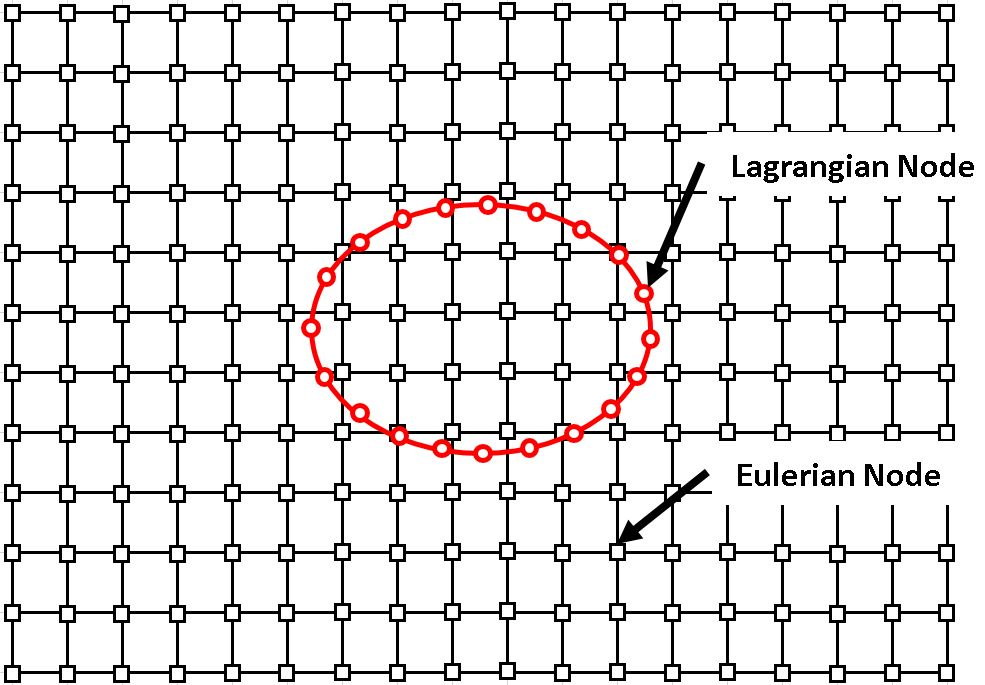
\includegraphics[width=7.00cm]{Chapter_4/figure/lagrangian_and_eulerian_nodes.jpg}
    \caption{Eulerian and Lagrangian nodes for representing the fluid and solid domains. The Eulerian and Lagrangian nodes are represented by squares and circles, respectively.}
    \label{fig:C4_lagrangianAndEulerianDomain}
\end{figure}
%
The forcing function in the penalization method is calculated at the \emph{Eulerian} nodes and is applied to computational nodes inside the solid boundary using a step function as shown in Equation \eqref{eq:C4_penalizationForcingFunction}.
%
\begin{equation}\label{eq:C4_penalizationForcingFunction}
    \mathbf{f} = -\mathcal{S}(\mathcal{X}(b)) \kappa \mathbf{u}
\end{equation}
%
Where $\mathcal{S}$ is the step function, $\mathcal{X}$ defines the relative location of the computational nodes inside the domain to the IB boundary, $\kappa$ is the penalization parameter, and $\mathbf{u}$ is the fluid velocity. Using this forcing function, the governing equation \eqref{eq:C4_NS} is rewritten as shown in Equation \eqref{eq:C4_NSwithPenalization}.
%
\begin{equation}\label{eq:C4_NSwithPenalization}
    \frac{\partial \mathbf{u}}{\partial t} + \mathbf{u} \cdot \nabla \mathbf{u} = 
    -\frac{\nabla P}{\rho} + \mu \nabla^2 \mathbf{u} -\mathcal{S}(\mathcal{X}(b)) \kappa \mathbf{u}
\end{equation}
%
As mentioned in Chapter \ref{ch:sensitivityAnalysis}, to derive the continuum sensitivity formulation, the governing equation of \eqref{eq:C4_NSwithPenalization} is differentiated with respect to the design variable, $b$. The step function $\mathcal{S}$'s derivative is the Dirac delta function, which is singular and cannot be used to solve the governing equations in a numerical framework. Therefore, a regularized Heaviside function, $\mathcal{H}$, will be employed instead of the step function for penalizing the governing equation. The effect of this function on the simulation results and sensitivity formulation will be discussed in the following sections.

In the virtual boundary method, the forcing function is calculated at the \emph{Lagrangian} nodes.
%
\begin{equation}\label{eq:C3_feedbackForcingFunction}
    \mathbf{f}(\mathbf{X}, t) = 
    \alpha \int_0^t \left[ \mathbf{u}(\mathbf{X}, \tau) - \mathbf{V}(\mathbf{X}, \tau) \right] d\tau + 
    \beta \left[ \mathbf{u}(\mathbf{X}, \tau) - \mathbf{V}(\mathbf{X}, \tau) \right]
\end{equation}
%
Where $\mathbf{u}(\mathbf{X}, t)$ is the fluid's velocity at the Lagrangian points $\mathbf{X}$ and $\mathbf{V}(\mathbf{X}, t)$ is the desired velocity at the Lagrangian point. For the no-slip boundary condition at the solid boundary, the desired velocity $\mathbf{V}(\mathbf{X}, t)$ is zero at each of the Lagrangian points. The Eulerian nodes, where the fluid's governing equation is solved, does not necessarily coincide with the Lagrangian points. Moreover, the forcing functions that are evaluated at the Lagrangian nodes need to be mapped to the Eulerian nodes where the governing equations for the fluid are solved. As mentioned in Chapter \ref{ch:immersedBoundary}, different mapping functions are used for transferring data between the Lagrangian and Eulerian nodes. However, none of these functions are continuously differentiable as required for the continuum sensitivity analysis. To address this issue, a regularized delta function is introduced.
% ============================================================================
\section{Regularized Heaviside/Delta Function}\label{sec:C4_RHandRDfunction}
The Regularized Heaviside (RH) function is a step function that is smoothened so that its derivative can be calculated numerically. The RH function is also known as sigmoid function in mathematics and is characterized as real-valued and differentiable, having either a non-negative or non-positive first derivative. There are a pair of horizontal asymptotes as $x \rightarrow \pm \infty$. The RH function is used instead of the step function to penalize the governing equation.  Several different RH functions defined in Equation \eqref{eq:C4_regularizedHeavisideFunctionFormulas} are shown in Figure \ref{fig:C4_heavisideFunctionExample}.
%
\begin{subequations}\label{eq:C4_regularizedHeavisideFunctionFormulas}
\begin{align}
    \mathcal{H}_1 &= \frac{1}{2} + \frac{1}{\pi} \arctan \left( x \right) \\
    \mathcal{H}_2 &= \frac{1}{1 + e^{-x}} \\
    \mathcal{H}_3 &= e^{-e^{-x}} \\
    \mathcal{H}_4 &= \frac{1 + \tanh(x)}{2}
\end{align}
\end{subequations}

\begin{figure}[H]
    \centering
    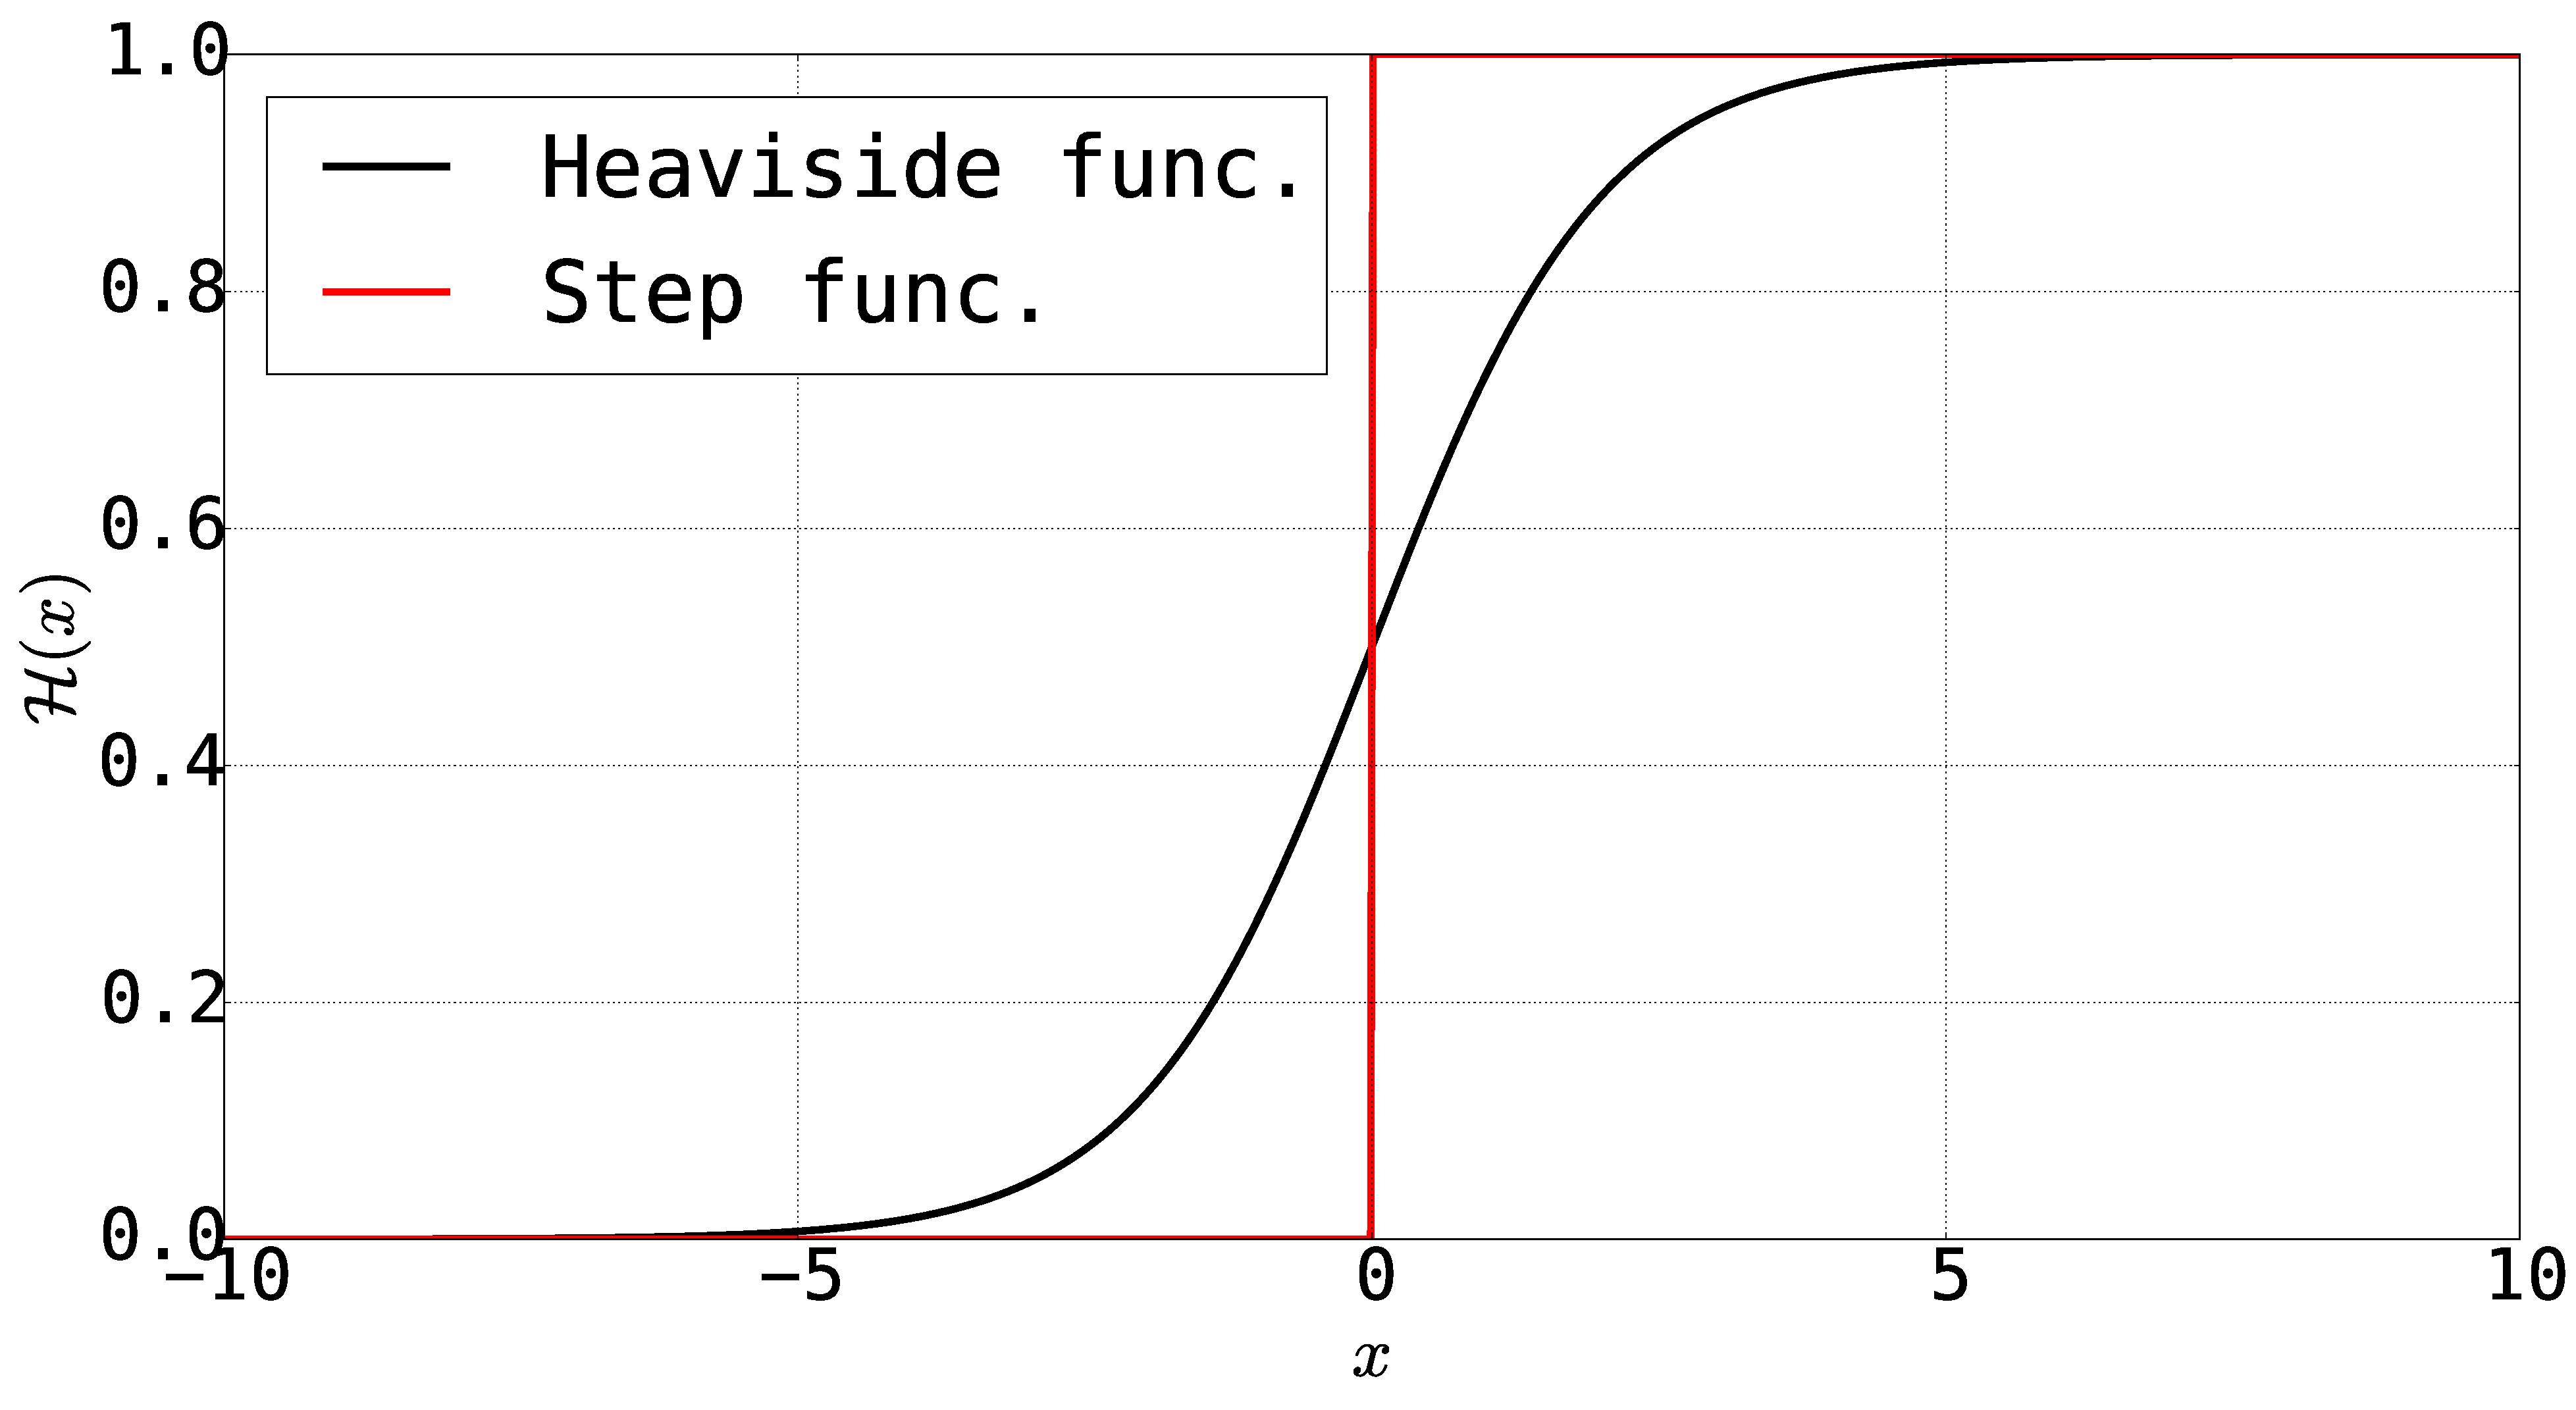
\includegraphics[width=12.00cm]{Chapter_4/figure/heaviside_function_example.eps}
    \caption{Comparison of different regularized Heaviside functions ($\mathcal{H}_i$) and step function ($\mathcal{S}$).}
    \label{fig:C4_heavisideFunctionExample}
\end{figure}
%
As shown in Figure \ref{fig:C4_heavisideFunctionExample}, all RH functions, other than $\mathcal{H}_3$, are symmetric around $x = 0$. This symmetry is required since the line $x = 0$ defines the boundary of the solid domain and accurate representation of the boundary requires the force terms to have same amount of information from both side of the boundary. By using an asymmetric definition for the RH function, the force term will be biased only on information from one side of the boundary. In this work, the RH function selected is $\mathcal{H}_4 = \dfrac{1 + \tanh(x)}{2}$, since it gives the fastest transition from $0$ to $1$. This transition is further controlled by adding the control parameter $\eta$ to the RH function definition as shown in Equation \eqref{eq:C4_heavisideFunction}. The effect of the control parameter on the RH function is shown in Figure \ref{fig:C4_heavisideFunctionWithControlParamter}. As shown in Figure \ref{fig:C4_heavisideFunctionWithControlParamter}, the transition region is reduced by increasing the control parameter. Using this feature, the smearing effect of penalization method can be reduced near the boundaries.
%
\begin{equation}\label{eq:C4_heavisideFunction}
    \mathcal{H} = \frac{1 + \tanh(x / \eta)}{2}
\end{equation}
%
%
\begin{figure}[H]
    \centering
    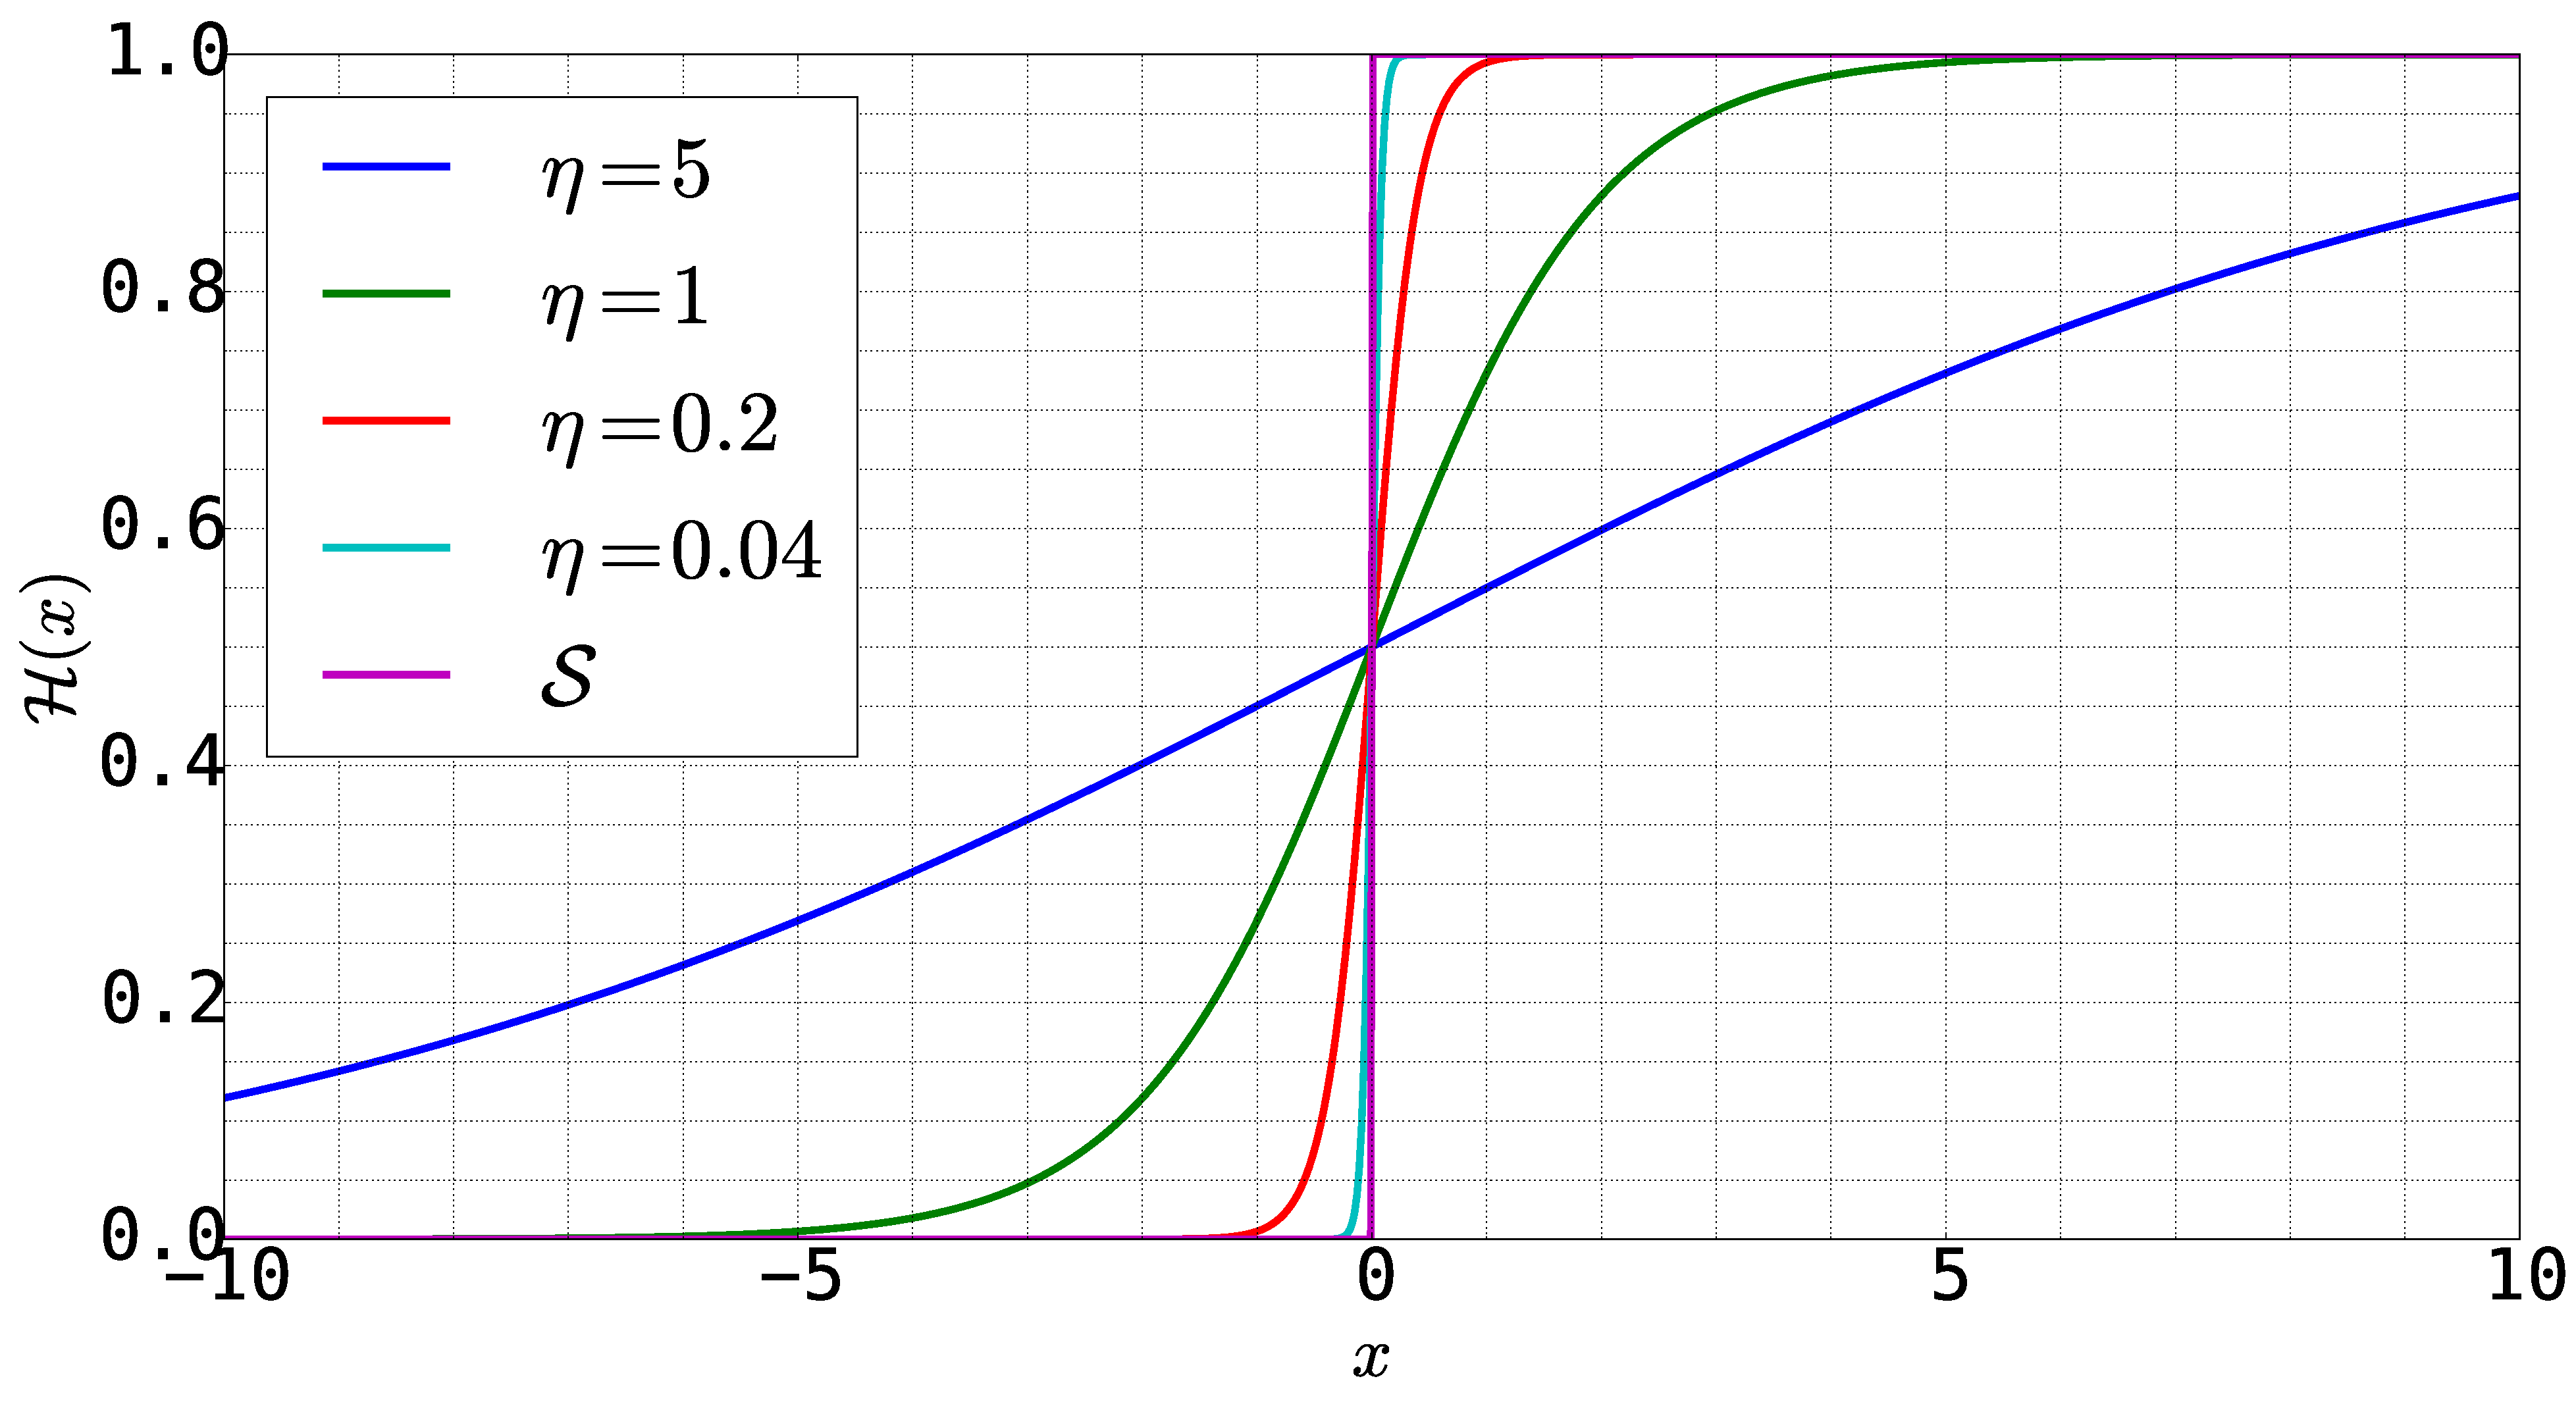
\includegraphics[width=12.00cm]{Chapter_4/figure/heaviside_function_with_control.eps}
    \caption{Effect of control parameter $\eta$ on the RH function.}
    \label{fig:C4_heavisideFunctionWithControlParamter}
\end{figure}
%
The penalized NS equation using the RH function of Equation \eqref{fig:C4_heavisideFunctionExample} is continuous and can be differentiated to derive the continuum sensitivity equations. The free parameter is defined based on the desired change of the RH function within a particular range as shown in Equation \eqref{eq:C4_etaGuideForRHfunction}.
%
\begin{equation}\label{eq:C4_etaGuideForRHfunction}
    \eta = \frac{R}{2 \tanh^{-1} (p)}
\end{equation}
%
Where $R$ is the distance that the $p$ percentage of the RH function occurs. For example, if it is required for the RH function to change 99 percent (p = 0.99) within length of 0.01 ($R = 0.01$), the required $\eta$ is calculated as $0.0018$ using Equation \eqref{eq:C4_etaGuideForRHfunction}.

For IB simulations incorporating the virtual boundary method, the Regularized Delta (RD) function is a substitute used for transferring data between the Lagrangian and Eulerian nodes. In mathematics, the Dirac delta function is defined as the derivative of the unit step function. To be consistent with the mathematical formulation, the RD function is calculated by differentiating the RH functions of Equation \eqref{eq:C4_regularizedHeavisideFunctionFormulas} as shown in Equation \eqref{eq:C4_regularizedDeltaFunctionFormulas}. These RD functions are plotted in Figure \ref{fig:C4_deltaFunctionExample}.
%
\begin{subequations}\label{eq:C4_regularizedDeltaFunctionFormulas}
\begin{align}
    \mathcal{D}_1 &= \frac{1}{\pi \left(x^{2} + 1\right)} \\
    \mathcal{D}_2 &= \frac{e^{- x}}{\left(1 + e^{- x}\right)^{2}} \\
    \mathcal{D}_3 &= \frac{e^{- x}}{e^{e^{- x}}} \\
    \mathcal{D}_4 &= - \frac{\tanh^{2}{\left (x \right )} + 1}{2}
\end{align}
\end{subequations}
%
%
\begin{figure}[H]
    \centering
    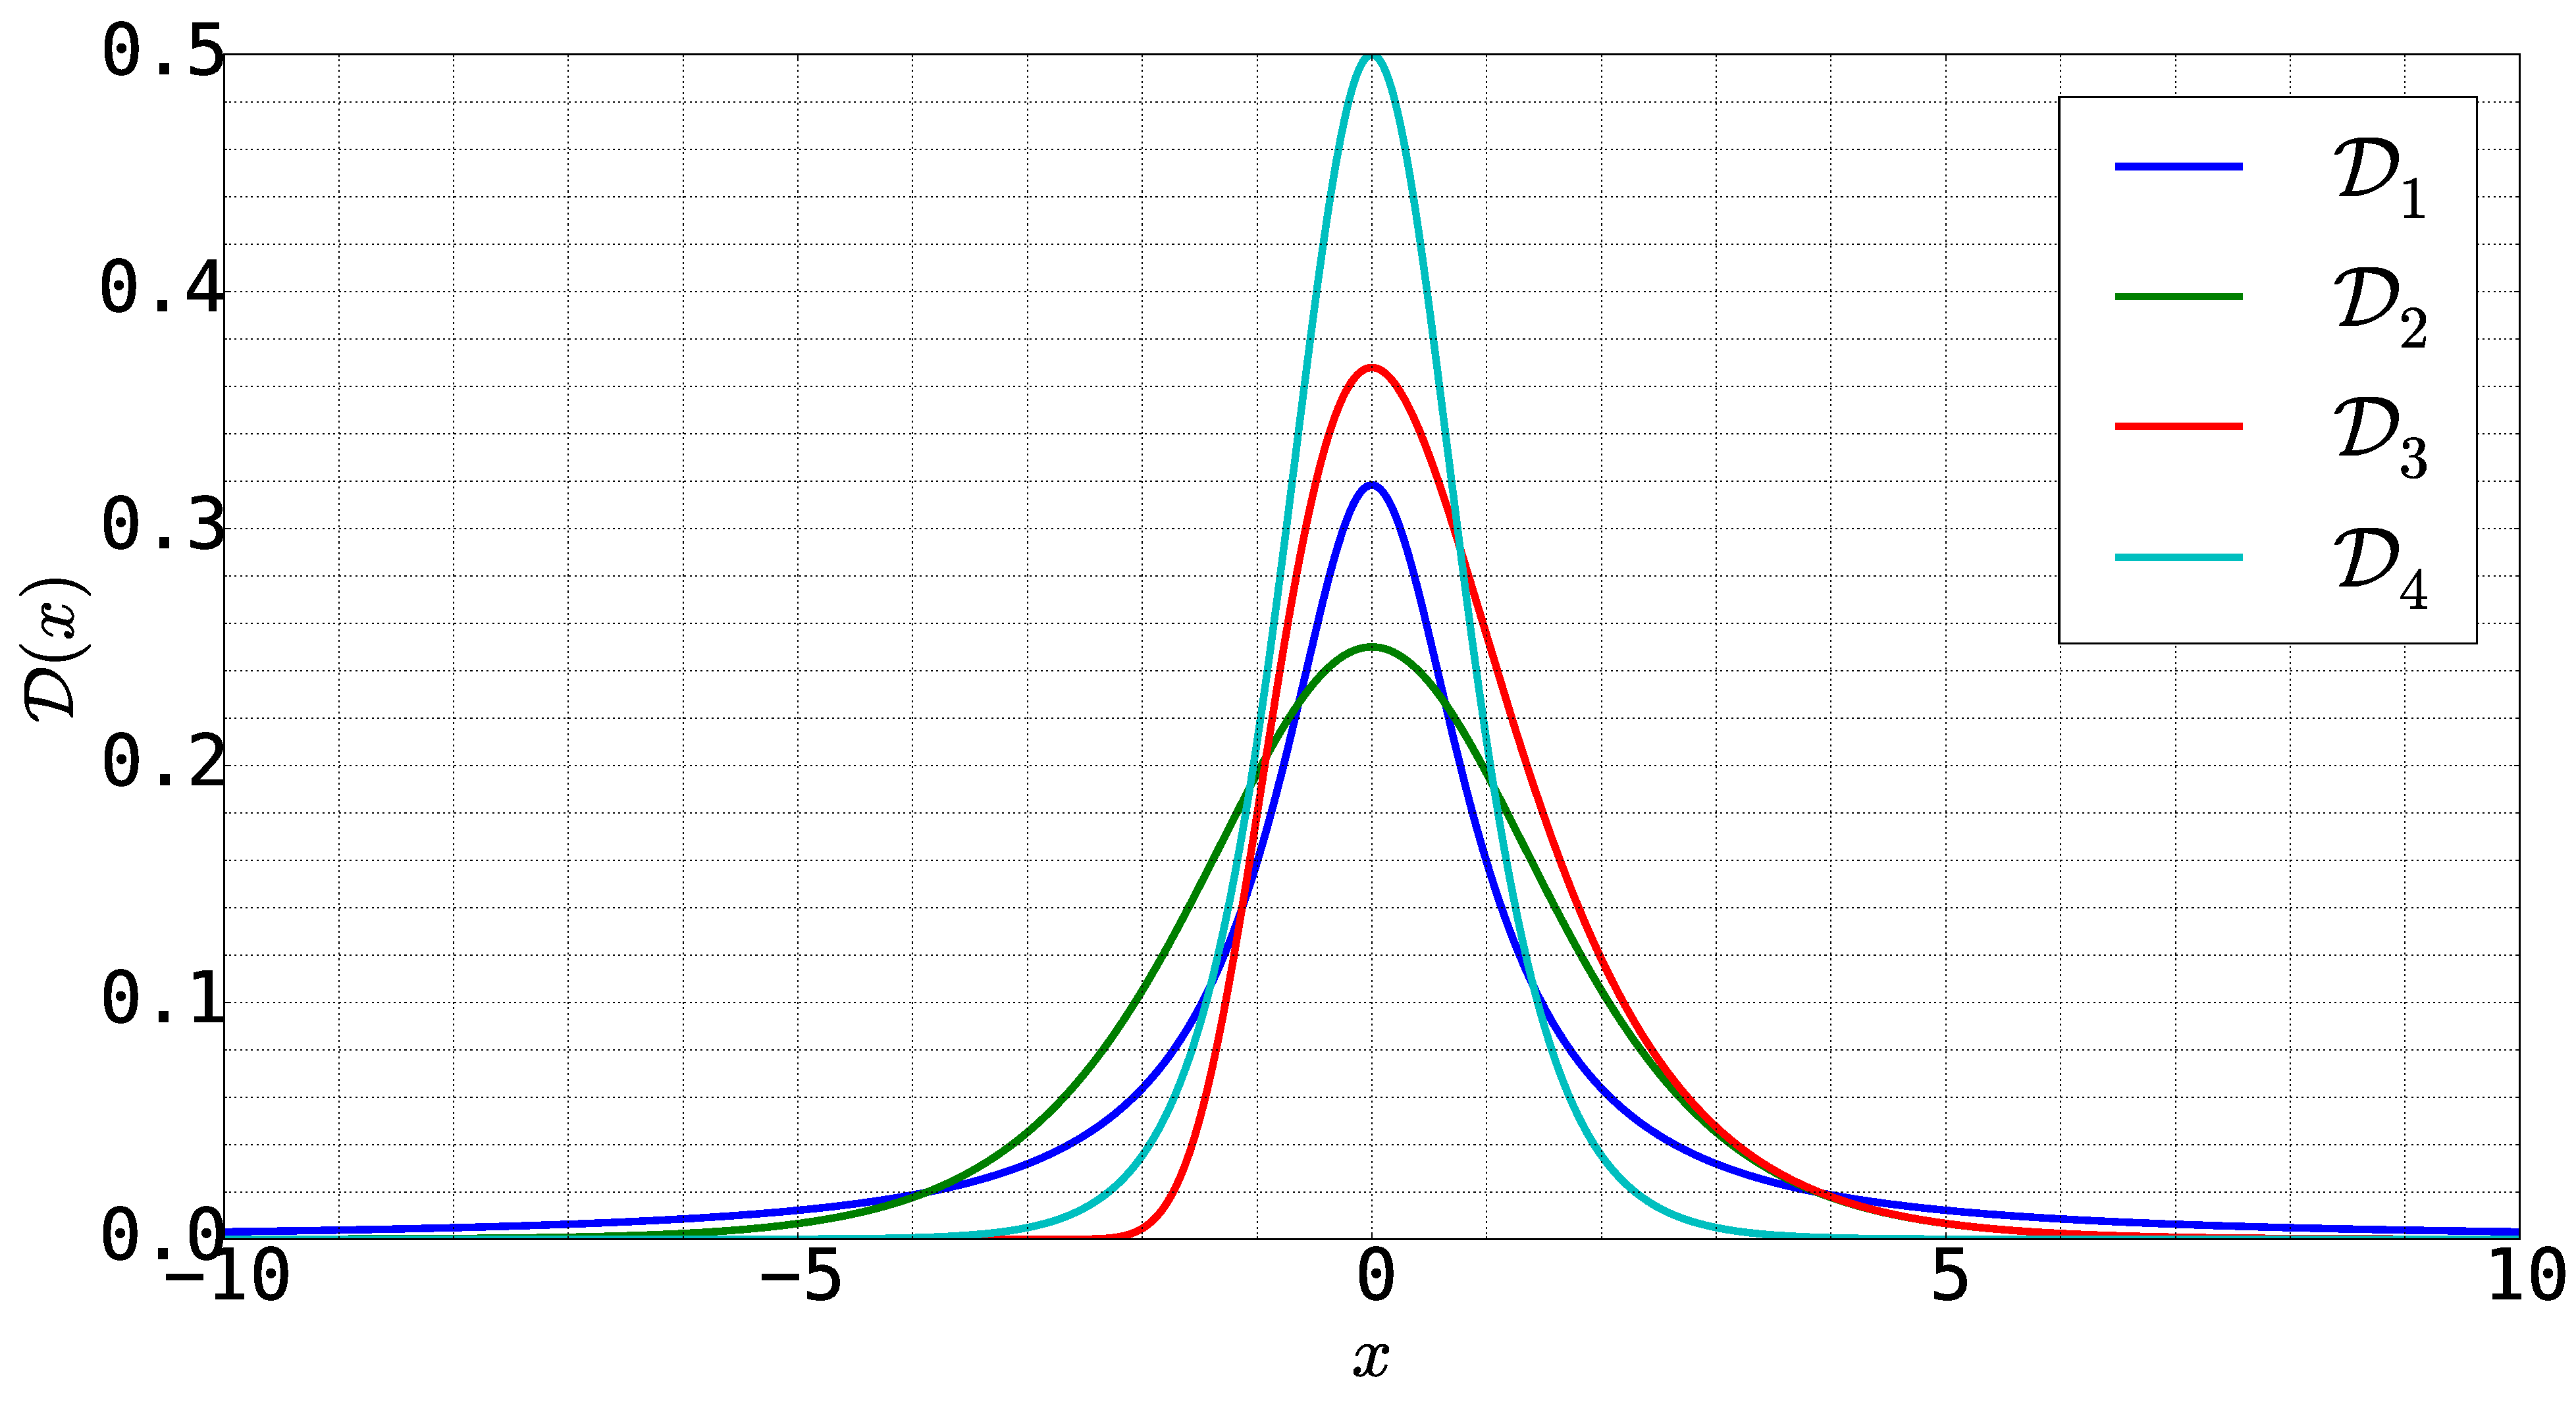
\includegraphics[width=12.00cm]{Chapter_4/figure/delta_function_example.eps}
    \caption{Comparison between different regularized delta functions ($\mathcal{D}_i$). The integral of all these functions over $x\in(-\infty, \infty)$ is equal to one.}
    \label{fig:C4_deltaFunctionExample}
\end{figure}
%
RD functions $\mathcal{D}_2$ and $\mathcal{D}_3$ exhibit instability issues due to different powers of the exponential in the numerator and denominator and $\mathcal{D}_1$ does not have a required sharpness expected from an RD function. Therefore, in this work, the RD function $\mathcal{D}_4$ is selected for implementation in the virtual boundary method. The sharpness of this RD function is further controlled by using the $\eta$ function as used in the definition of the corresponding RH function. This is defined in Equation \eqref{eq:C4_deltaFunction}. The RD function for different values of $\eta$ are shown in Figure \ref{fig:C4_deltaFunctionWithControlParamter}.
%
\begin{equation}\label{eq:C4_deltaFunction}
    \mathcal{D} = \dfrac{1}{\eta} \left( \dfrac{-\tanh^{2}{\left (\dfrac{x}{\eta} \right )} + 1}{2} \right)
\end{equation}
%
%
\begin{figure}[H]
    \centering
    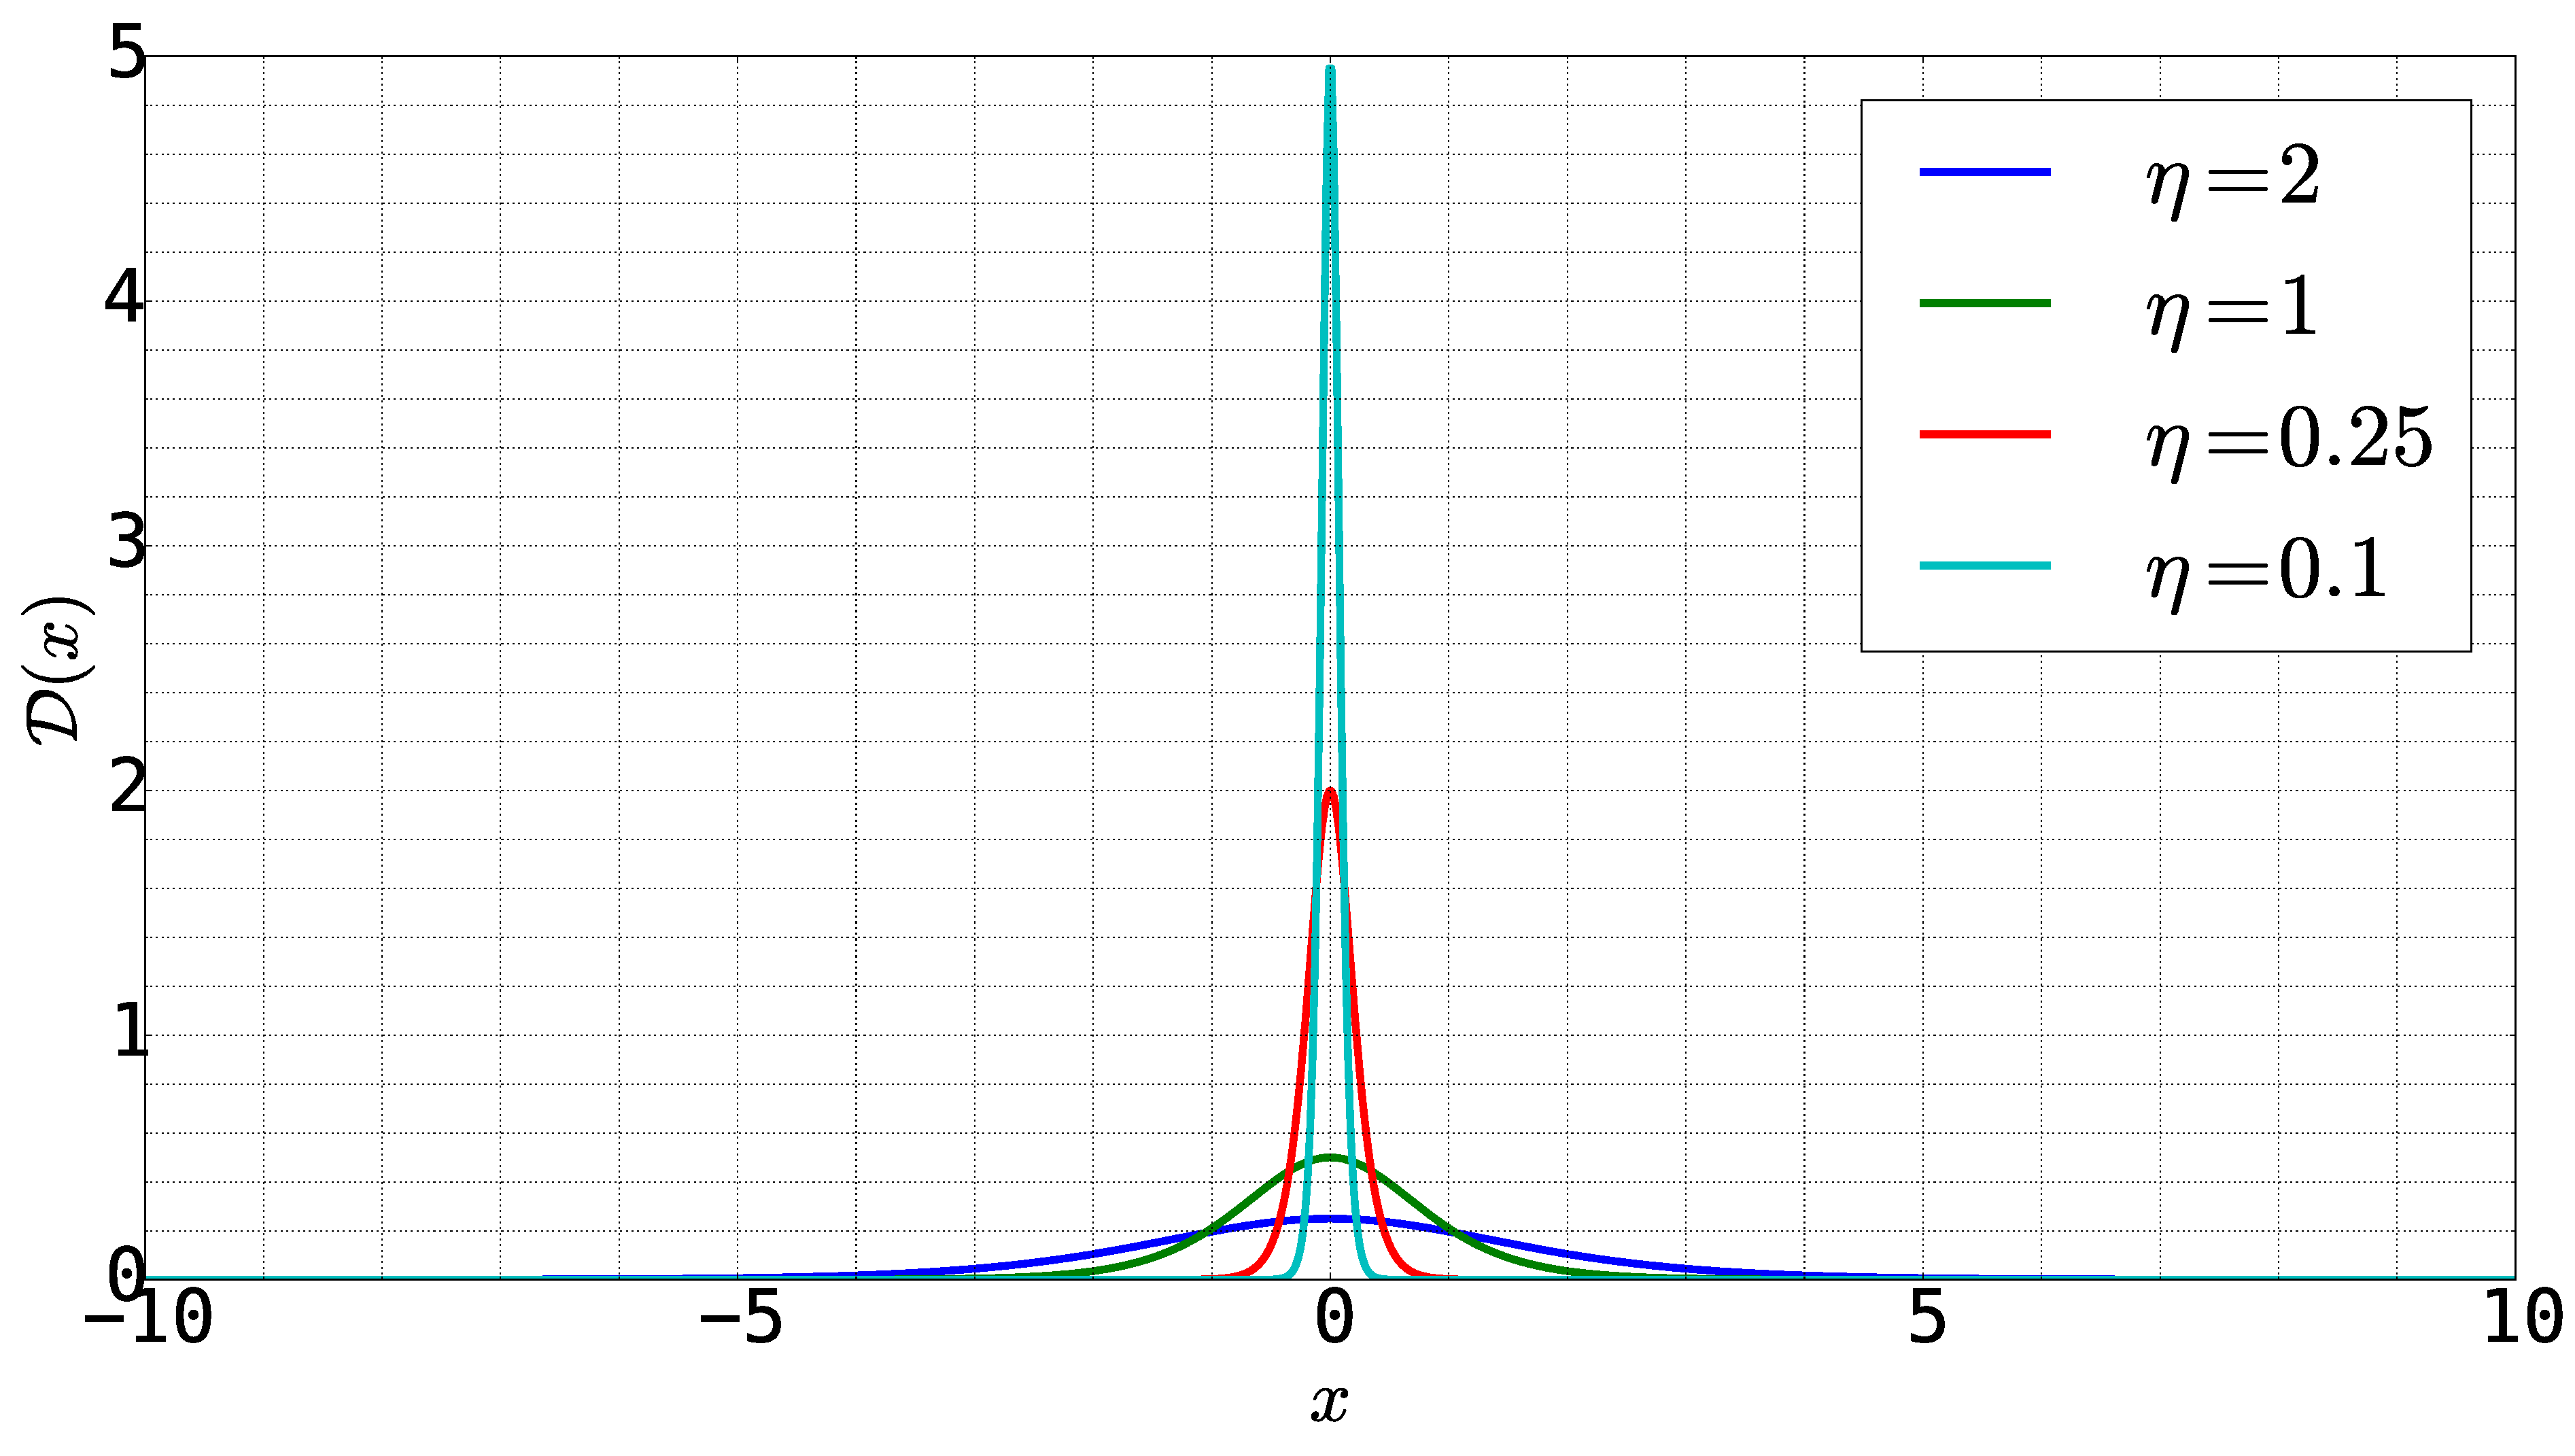
\includegraphics[width=12.00cm]{Chapter_4/figure/delta_function_with_control.eps}
    \caption{Effect of control parameter $\eta$ on the RD function.}
    \label{fig:C4_deltaFunctionWithControlParamter}
\end{figure}
%
As shown in Figure \ref{fig:C4_deltaFunctionWithControlParamter}, the RD function has continuous derivatives. This enables the virtual boundary method to be used for sensitivity calculation by providing differentiable governing equations. For the RD function, the free parameter is calculated by selecting how fast the RD function decays when moving further from its symmetry axis. The free parameter for the RD function is defined in Equation \eqref{eq:C4_etaGuideForRDfunction}.
%
\begin{equation}\label{eq:C4_etaGuideForRDfunction}
    \eta = \frac{R}{\tanh^{-1} (\sqrt{1 - p})}
\end{equation}
%
The RD function drops to $p$ percentage of its value at the symmetry axis at distance $R$. For example, for the RD function value to drop 99 percent ($p = 0.99$) within 0.01 ($R = 0.01$) of the symmetry axis of the RD function, the $\eta$ value is calculated as $0.0033$ based on Equation \eqref{eq:C4_etaGuideForRDfunction}.
% ============================================================================
\section{Sensitivity Analysis Formulation}
In this section, the sensitivity equations are derived for IB representation of solid boundaries. Two separate IB methods are selected for the sensitivity analysis, the penalization method, and the virtual boundaries method. The direct sensitivity equations for design variables that control the shape of the IB are derived for these analysis and later applied on two different demonstration problems. 

As mentioned in Chapter \ref{ch:sensitivityAnalysis}, the direct method for sensitivity analysis is preferred when the number of design variables are less than the number of functions for which the sensitivities are calculated for. For this approach, the governing equations are differentiated with respect to the arbitrary shape design variable, $b$.

For the penalization method, a level-set definition of the solid boundary is used to assign penalization factors to the nodes. As defined in Chapter \ref{ch:immersedBoundary}, the boundary is defined using an analytical function, $\mathcal{X}$, that depends on the shape design variable. The governing equation for flow over the immersed boundaries using penalization method is written using the RH function:
%
\begin{equation}\label{eq:C4_NSwithPenalizationIB}
    \frac{\partial \mathbf{u}}{\partial t} + \mathbf{u} \cdot \nabla \mathbf{u} = 
    -\frac{\nabla P}{\rho} + \nu \nabla^2 \mathbf{u} -\mathcal{H}(\mathcal{X}(b)) \kappa \mathbf{u}
\end{equation}
%
Equation \eqref{eq:C4_NSwithPenalizationIB} is differentiated with respect to design variable $b$ to derive the continuum sensitivity equations. The symbol $(\text{ })'$ represents $\partial /\partial b$ in the sensitivity equation \eqref{eq:C4_NSwithPenalizationIBsensitivity}.
%
\begin{equation}\label{eq:C4_NSwithPenalizationIBsensitivity}
    \frac{\partial \mathbf{u}'}{\partial t} +
    \mathbf{u}' \cdot \nabla \mathbf{u} + \mathbf{u} \cdot \nabla \mathbf{u}' = 
    -\frac{\partial P'}{\rho} + 
    \nu \nabla^2 \mathbf{u}' - 
    \underbrace{\frac{\partial \mathcal{H}}{\partial \mathcal{X}} \frac{\partial \mathcal{X}}{\partial b} \kappa \mathbf{u}}_\text{effect of shape change} - 
    \mathcal{H}(\mathcal{X}) \kappa \mathbf{u}'
\end{equation}
%
Equation \eqref{eq:C4_NSwithPenalizationIBsensitivity} is solved for velocity and pressure sensitivities ($\mathbf{u}'$, $P'$) by knowing the values of $\mathbf{u}$ from the analysis. As shown in Equation \eqref{eq:C4_NSwithPenalizationIBsensitivity}, the effect of shape change is introduced to the sensitivity equation through the derivative of the RH function. $\partial \mathcal{H}/\partial \mathcal{X}$ is easily calculated by analytically differentiating the RH function with respect to $\mathcal{X}$. The evaluation of $\partial \mathcal{X}/\partial b$ is also straight forward, since it was assumed that the solid boundary is defined analytically. The boundary conditions for Equation \eqref{eq:C4_NSwithPenalizationIB} are often independent of the shape design variables. Therefore, their derivative is typically zero. This enables us to solve the governing Equation of \eqref{eq:C4_NSwithPenalizationIBsensitivity} for the sensitivity response.

Sensitivity implementation for the virtual boundary method is more demanding compared to the penalization method. Using the RD function, the NS equation using virtual boundary method for solid boundary definition is written as shown in Equation \eqref{eq:C4_NSwithvirtualBoundaryIB}.
%
\begin{align}\label{eq:C4_NSwithvirtualBoundaryIB}
    \frac{\partial \mathbf{u}}{\partial t} + 
    \mathbf{u} \cdot \nabla \mathbf{u} = 
    &-\frac{\nabla P}{\rho} + 
    \nu \nabla^2 \mathbf{u} + \nonumber \\
    &\left\{
    \alpha
    \int_0^t
    \left[
        \int \mathbf{u}(\mathbf{x}, \tau) \mathcal{D}(\mathbf{x} - \mathbf{X}) d\mathbf{x} - \mathbf{V}(\mathbf{X}, \tau)
    \right] d\tau \right.
    + \nonumber \\
    &
    \left.
    \beta
    \int \mathbf{u}(\mathbf{x}, t) \mathcal{D}(\mathbf{x} - \mathbf{X}) d\mathbf{x} - \mathbf{V}(\mathbf{X}, t)
    \right\} \mathcal{D}(\mathbf{x} - \mathbf{X})
\end{align}
%
where $\mathbf{V}(\mathbf{X}, t)$ is the desired velocity at the Lagrangian point on the solid boundary and $\int \mathbf{u}(\mathbf{x}, t) \mathcal{D}(\mathbf{x} - \mathbf{X}) d\mathbf{x}$ is the current velocity at the Lagrangian node, $\mathbf{X}$, on the solid boundary calculated from the Eulerian nodes on the fluid's domain. To transfer the forces back to the Eulerian nodes, the same RD function is used as shown in Equation \eqref{eq:C4_NSwithvirtualBoundaryIB} by $\mathcal{D}(\mathbf{x} - \mathbf{X})$ where the term in the parenthesis ($\mathbf{x} - \mathbf{X}$) is responsible for casting the RD function at the location of the Lagrangian point $\mathbf{X}$. The maximum value for the RD function $\mathcal{D}$ is normalized to one. This is essential to have a conservative transformation between the Eulerian and Lagrangian computational nodes. The mapping procedure is illustrated in the following example.

Assume that the analytical function $y=x^2$ is evaluated at $9$ locations between $0$ and $1$. To know the function value at locations $X = 0.3321$ and $X = 0.5813$, that do not coincide with the location where the function is evaluated, it is required to use the following equation. We used the RD definition of Equation \eqref{eq:C4_deltaFunction} with $\eta = 0.1$ for this purpose.
%
\begin{equation}\label{eq:C4_euler2lagrange}
    y(X) = \sum_{i=1}^9 \mathcal{D}_i Y_i \Delta x_i
\end{equation}
%
Where the subscript $i$ is the number of points used to discretize the Delta function. This equation used the data from nodes around $X$ to calculate the function value. To convert the data at $X$ (Lagrangian node) back to the surrounding nodes where the original function was evaluated, the following equation is used.
%
\begin{equation}
    y(x) = y(X) \mathcal{D}(x - X)
\end{equation}
%
Where $\bar{\mathcal{D}}(x - X)$ is a constant vector. The transfer of data from Eulerian nodes to Lagrangian is shown in Figure \ref{fig:C4_euler2lagrangeExample}. In this figure, the original function is represented by the solid black line and the sampling locations are represented by black circles. The exact function value at the Lagrangian point is shown by a red circle and the calculated value from Equation \eqref{eq:C4_euler2lagrange} is shown by a blue cross. The numerical results for the comparison between the interpolated and actual values are shown in Table \ref{table:C4_euler2lagrangeExample}. The green squares represent the mapped back data to the Eulerian domain from the data at the Lagrangian point $X$ shown with a red circle in Figure \ref{fig:C4_euler2lagrangeExample}. As shown here, the data at Lagrangian nodes mainly affects the two closest Eulerian nodes. The effect of Lagrangian data at $X$ decreases by moving further from $X$. The mapping from the Lagrangian to Eulerian domain has larger error compared to the mapping from Eulerian to Lagrangian grid. However, since this is done in a loop, the error diminishes as the simulation continues in time.
%
\begin{figure}[H]
    \centering
    \subfigure[$X = 0.3321$]
    {
    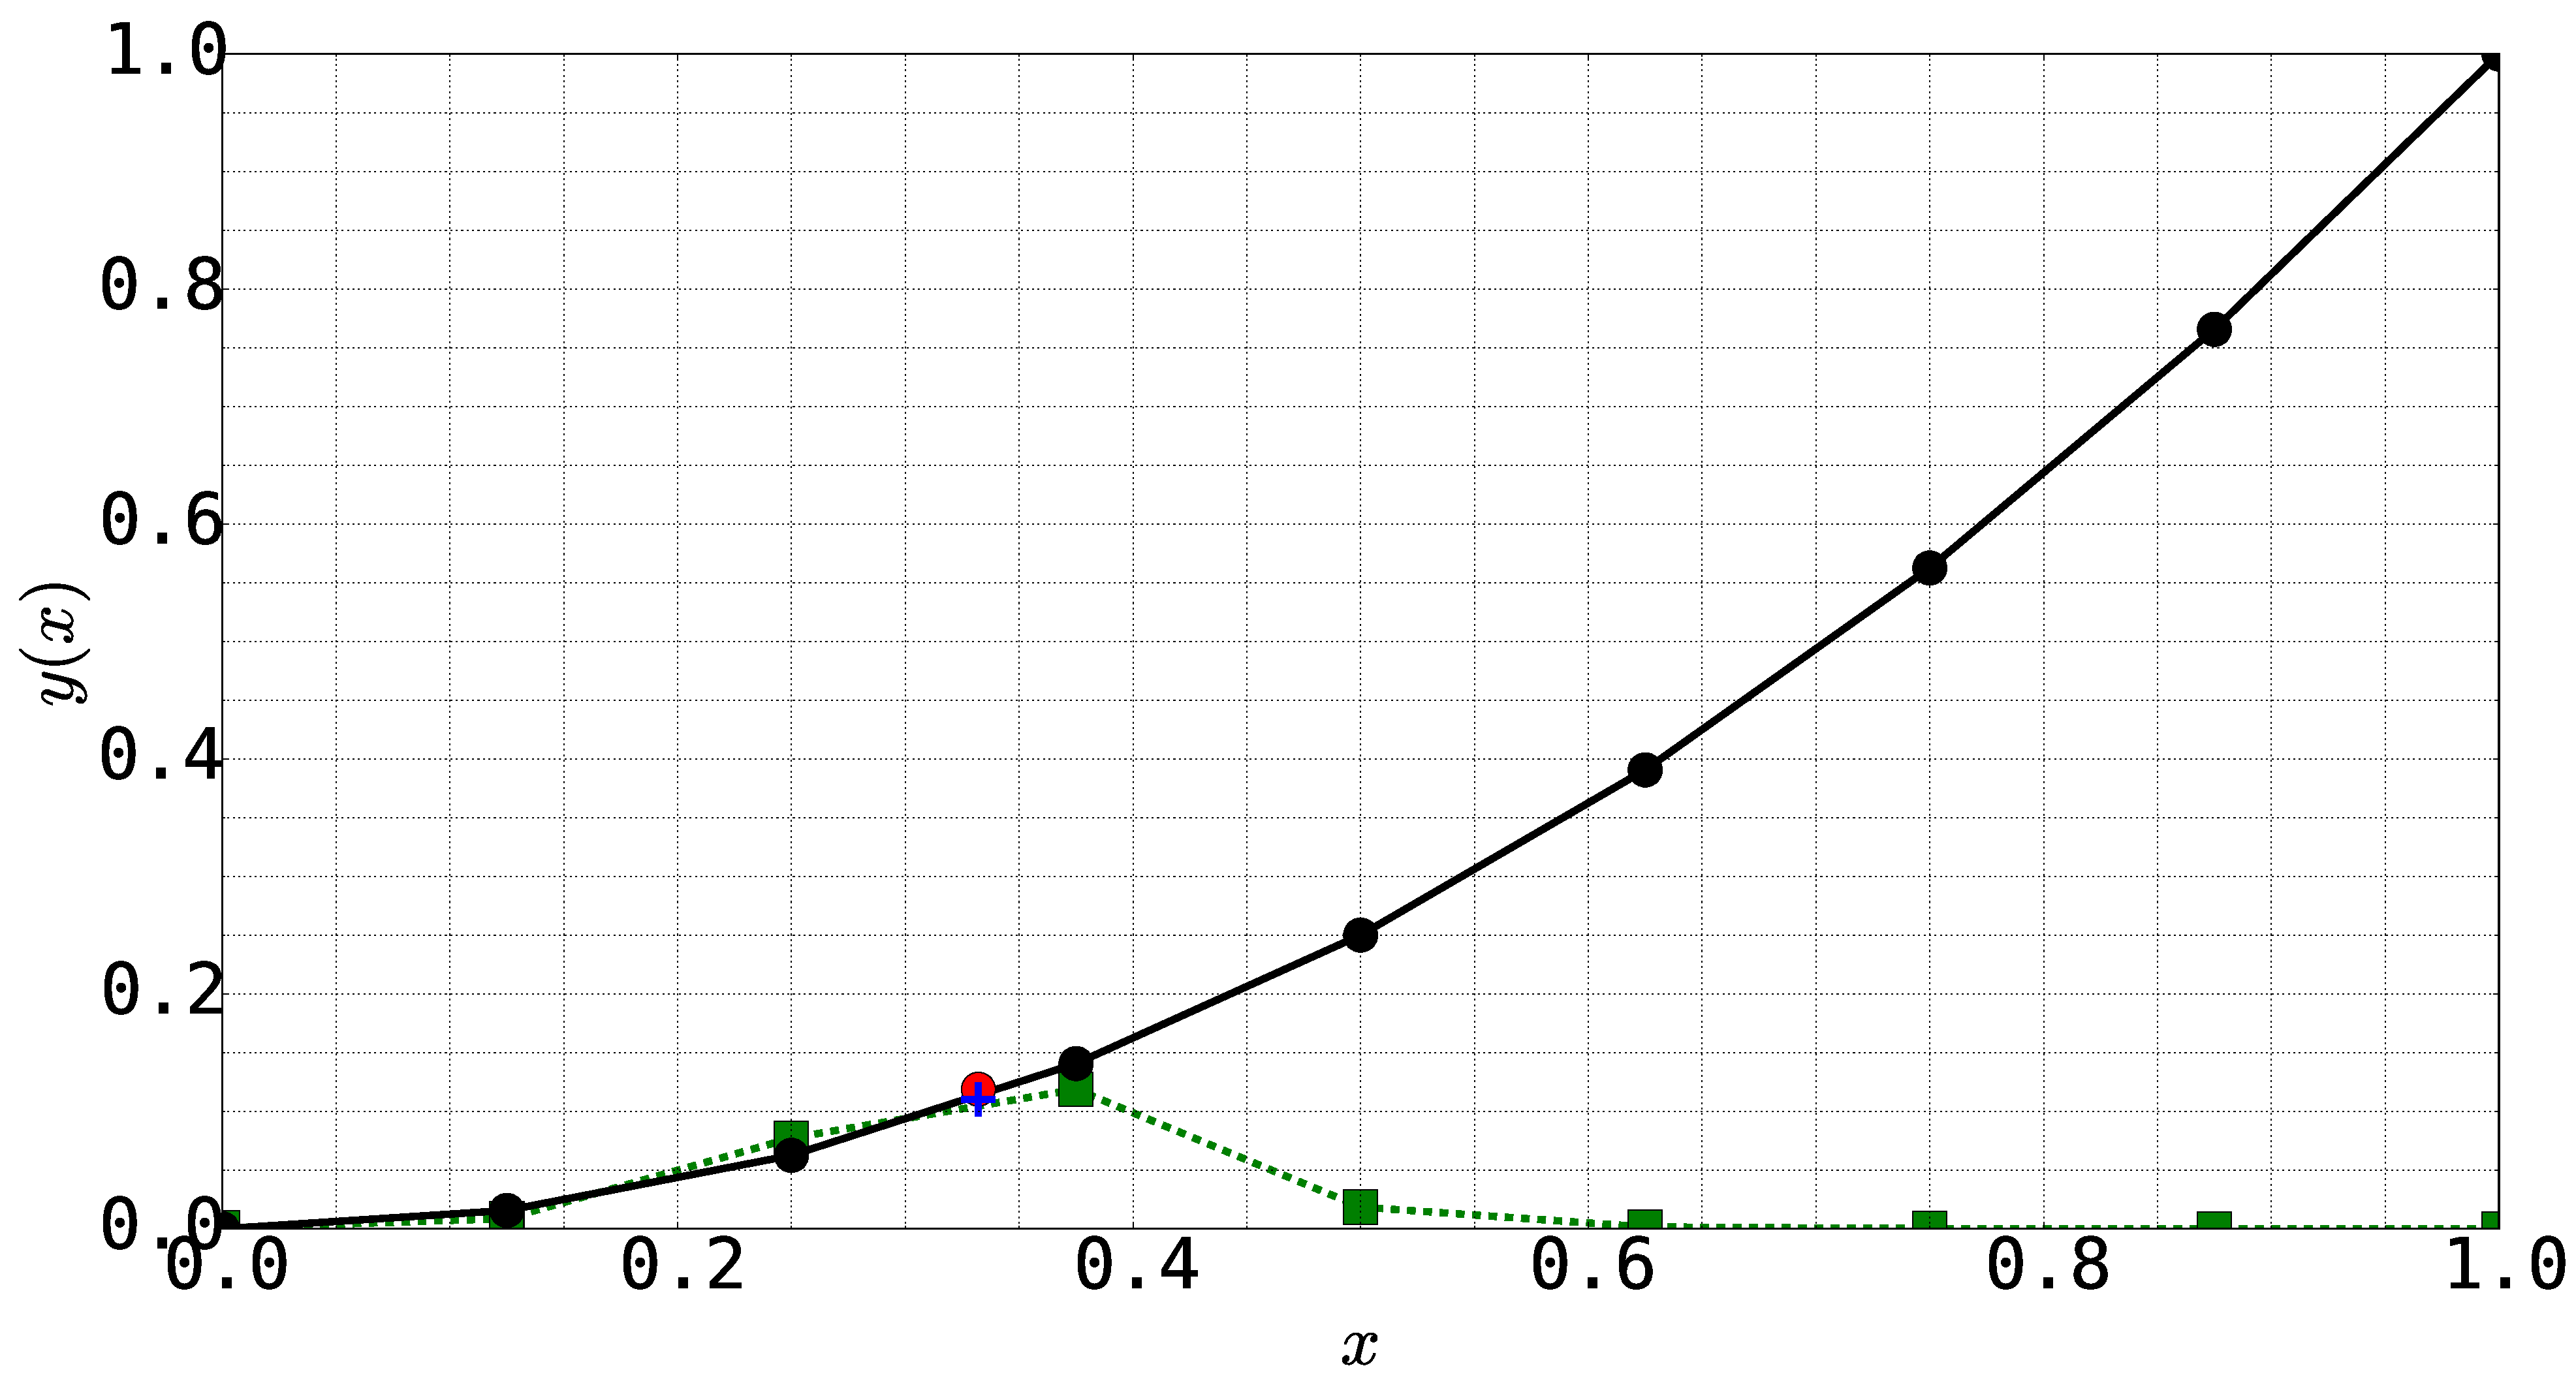
\includegraphics[width=6.5cm]{Chapter_4/figure/euler2lagrange_example_03321.eps}
    }
    \quad
    \subfigure[$X = 0.5813$]
    {
    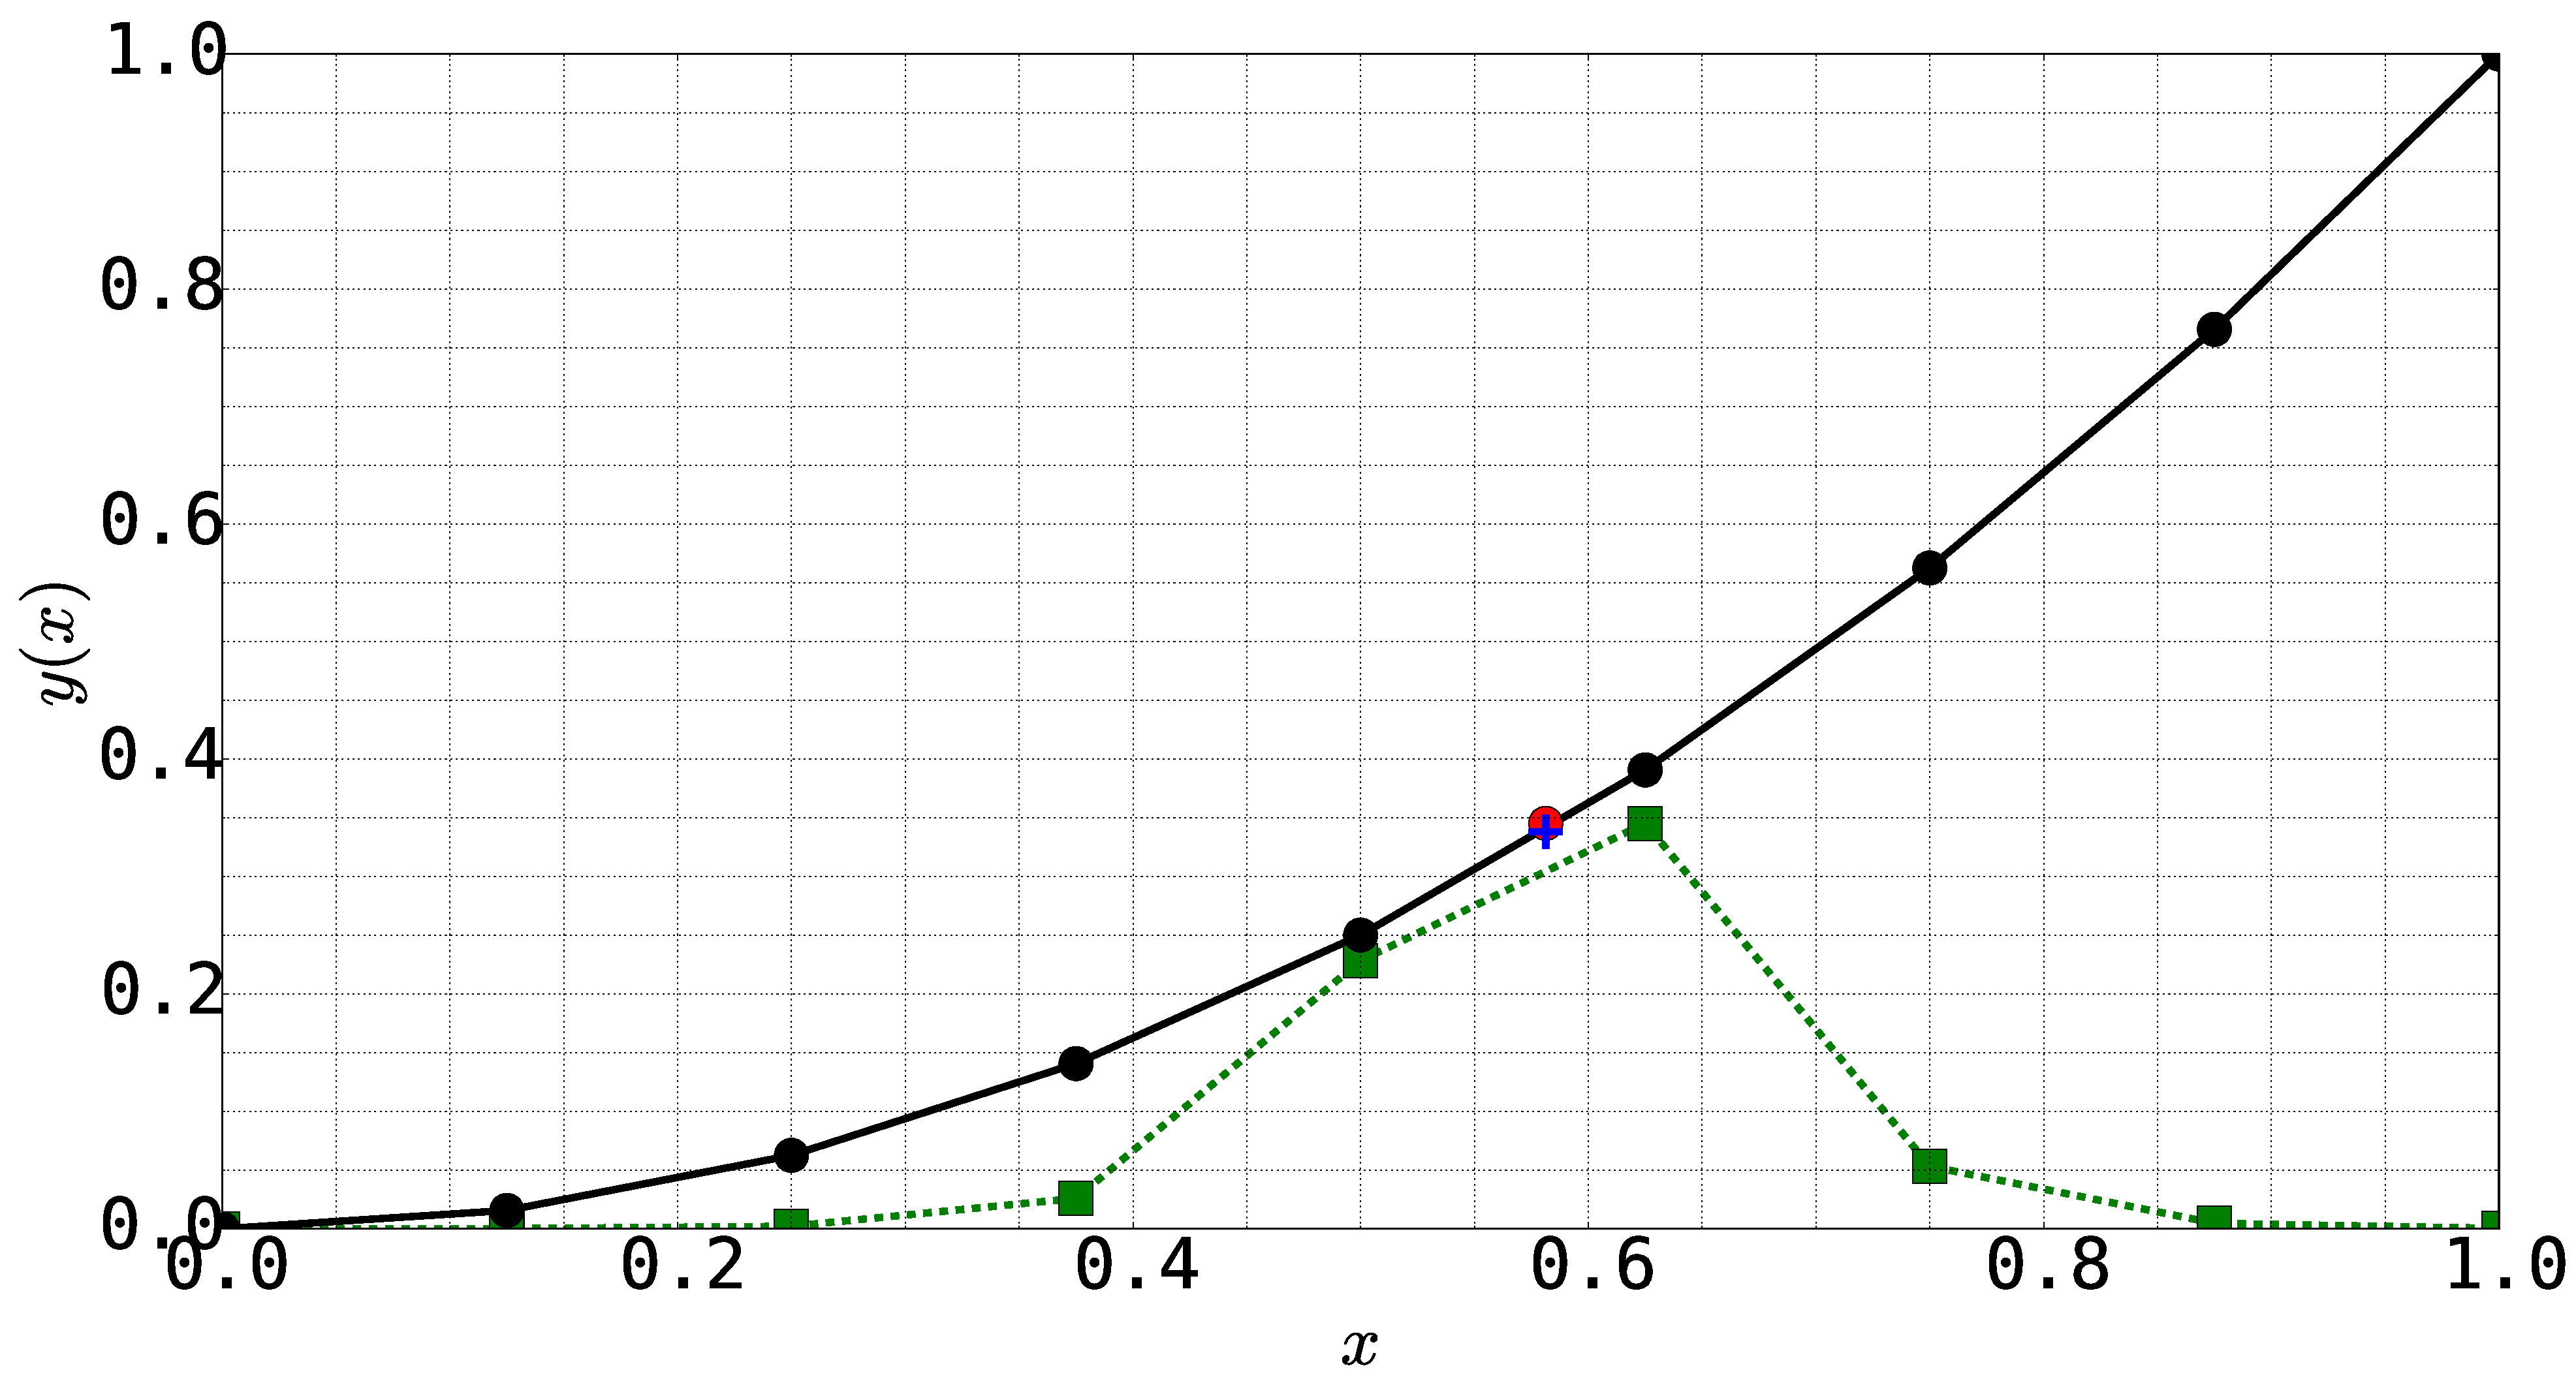
\includegraphics[width=6.5cm]{Chapter_4/figure/euler2lagrange_example_05813.eps}
    }
    \caption{Results mapping between the Eulerian and Lagrangian computational nodes.}
    \label{fig:C4_euler2lagrangeExample}
\end{figure}
%
%
\begin{table}[H]
\centering
\begin{tabular}{| c | c |}
    \hline
    Lagrangian node location ($X$) & Absolute error \\ \hline \hline
    0.3321 & 0.0077 \\ \hline
    0.5813 & 0.0021 \\ \hline
\end{tabular}
\caption{Comparison between the true and interpolated results using the RD function at arbitrary Lagrangian location, $X$.}
\label{table:C4_euler2lagrangeExample}
\end{table}
%
Using this continuous mapping between the Eulerian and Lagrangian domains, the governing equation \eqref{eq:C4_NSwithvirtualBoundaryIB} is differentiated with respect to design variable $b$ to derive the sensitivity equations. $(\text{ })'$ is used instead of the sensitivity operator, $\partial/\partial b$.
%
\begin{align}\label{eq:C4_NSwithvirtualBoundaryIBsensitivity}
    \frac{\partial \mathbf{u}'}{\partial t} &+ 
    \mathbf{u}' \cdot \nabla \mathbf{u} +
    \mathbf{u} \cdot \nabla \mathbf{u}' = 
    -\frac{\nabla P'}{\rho} + 
    \nu \nabla^2 \mathbf{u}' + \nonumber \\
    &\left\{
    \alpha
    \int_0^t
    \left[
        \int \mathbf{u}'(\mathbf{x}, \tau) \mathcal{D}(\mathbf{x} - \mathbf{X}) d\mathbf{x} + 
        \int \mathbf{u}(\mathbf{x}, \tau) \frac{\partial \mathcal{D}}{\partial X} \frac{\partial X}{\partial b} d\mathbf{x}
    \right] d\tau \right.
    + \nonumber \\
    &
    \left.
    \beta
    \int \mathbf{u}'(\mathbf{x}, t) \mathcal{D}(\mathbf{x} - \mathbf{X}) d\mathbf{x} +
    \int \mathbf{u}(\mathbf{x}, t) \frac{\partial \mathcal{D}}{\partial X} \frac{\partial X}{\partial b} d\mathbf{x}
    \right\} \mathcal{D}(\mathbf{x} - \mathbf{X}) + \nonumber \\
    &\left\{
    \alpha
    \int_0^t
    \left[
        \int \mathbf{u}(\mathbf{x}, \tau) \mathcal{D}(\mathbf{x} - \mathbf{X}) d\mathbf{x} - \mathbf{V}(\mathbf{X}, \tau)
    \right] d\tau \right.
    + \nonumber \\
    &
    \left.
    \beta
    \int \mathbf{u}(\mathbf{x}, t) \mathcal{D}(\mathbf{x} - \mathbf{X}) d\mathbf{x} - \mathbf{V}(\mathbf{X}, t)
    \right\}
    \frac{\partial \mathcal{D}}{\partial X} \frac{\partial X}{\partial b}
\end{align}
%
Equation \eqref{eq:C4_NSwithvirtualBoundaryIBsensitivity} is solved for the sensitivity response $\mathbf{u}'$, where $\mathbf{u}$ is known from the analysis results. The effect of shape change is introduced in the sensitivity equation through the derivative of the RD function, $\dfrac{\partial D}{\partial X} \dfrac{\partial X}{\partial b}$. The first term in this description is easily calculated since the RD function is known. The derivative of Lagrangian node location, $X$, to the design variable, $b$, is known since the solid boundary is defined analytically. The boundary conditions of Equation \eqref{eq:C4_NSwithvirtualBoundaryIB} are often design independent and have zero sensitivity. However, as showed in the work of Cross and Canfield \cite{cross2015local}, the order of which the boundaries are defined can greatly affect the accuracy of sensitivity results. This can be addressed by either using higher order methods to approximate the boundaries or using Spatial Gradient Reconstruction (SGR) technique of Cross and Canfield \cite{cross2014local}. In this work we used higher order boundary approximation to address this issue.

%\subsection{Adjoint Method}
%The adjoint method is preferred when the number of the functions the sensitivity is calculated for is less than the number of design variables. To derive the continuous adjoint sensitivity, the governing equation is defined as $\mathcal{R}(\mathbf{u}, \mathbf{b}) = 0$ and the function for which the sensitivities are calculated is defined as $h(\mathbf{u}, \mathbf{b})$. In these equations, $\mathbf{u}$ is the response variable, i.e. velocity, pressure, or displacement, and $\mathbf{b}$ is the design variable. To derive the adjoint formulation, the Lagrangian is defined as shown in Equation \eqref{eq:C4_lagrangianForAdjoint}. It should be noted that if $\mathbf{u}$ satisfies the governing equation, the Lagrangian, $\Gamma$, is equal to the function of interest. Therefore, its sensitivity is equal to the sensitivity of the Lagrangian.
%%
%\begin{equation}\label{eq:C4_lagrangianForAdjoint}
%    \Gamma(\mathbf{u}, \mathbf{b}) = h(\mathbf{u}, \mathbf{b}) + \lambda \mathcal{R}(\mathbf{u}, \mathbf{b})
%\end{equation}
%%
%Differentiating Equation \eqref{eq:C4_lagrangianForAdjoint} and rewriting the terms, results in the following equation. 
%%
%\begin{equation}
%    \frac{d \Gamma}{d b_i} = 
%    \frac{\partial h}{\partial b_i} + 
%    \left[ \frac{\partial h}{\partial \mathbf{u}} + \lambda \frac{\partial \mathcal{R}}{\partial b_i} \right]
%    \frac{\partial \textbf{u}}{\partial b_i} + 
%    \lambda \frac{\partial \mathcal{R}}{\partial b_i}
%\end{equation}
%%
%To avoid calculating $\dfrac{\partial \textbf{u}}{\partial b_i}$, its coefficient is set equal to zero. This results in Equation \eqref{eq:C4_adjointVectorDefinition} for the adjoint variable $\lambda$.
%%
%\begin{equation}\label{eq:C4_adjointVectorDefinition}
%    \lambda = -\left( \frac{\partial \mathcal{R}}{\partial \mathbf{u}} \right)^{-1} \frac{\partial h}{\partial \mathbf{u}}
%\end{equation}
%%
%By knowing the adjoint vector, the sensitivity of Lagrangian function, $\Gamma(\mathbf{u}, \mathbf{b})$, is written as shown in Equation \eqref{eq:C4_functionSensitivityAdjoint}
%%
%\begin{equation}\label{eq:C4_functionSensitivityAdjoint}
%    \frac{d \Gamma}{d b_i} = 
%    \frac{\partial h}{\partial b_i} + 
%    \lambda \frac{\partial \mathcal{R}}{\partial b_i}
%\end{equation}
%
%The adjoint formulation is implemented for a simple continuous system as defined in Figure \ref{fig:C4_stepBeamAdjoint}. The design variables are selected as the cross-sectional areas of the axial bars, $A_1$ and $A_2$. The length of the bars are chosen as $L_1$ and $L_2$ with a force applied at the tip, $F$. We are interested in the sensitivity of stress in the bar (1) with respect to the cross-sectional areas $A_1$ and $A_2$.
%
%\begin{figure}[H]
%    \centering
%    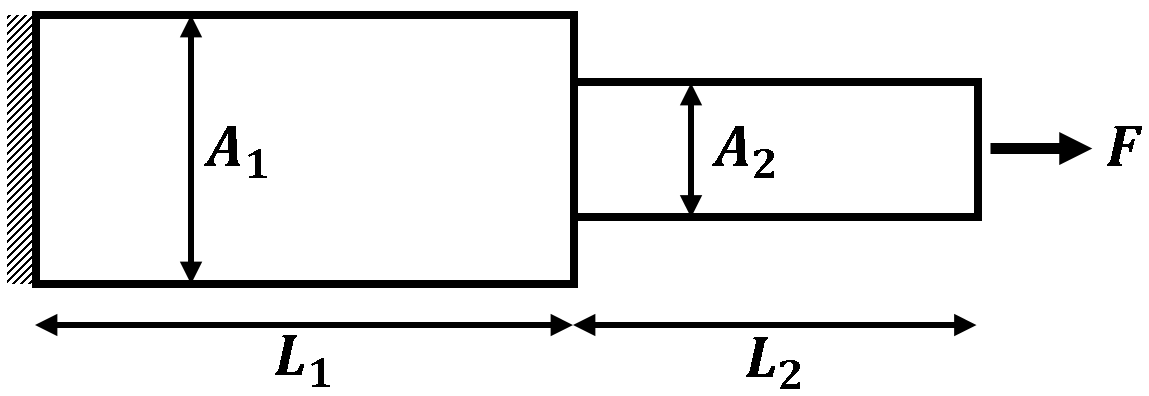
\includegraphics[width=7.00cm]{Chapter_4/figure/beam_adjoint_example_problem.png}
%    \caption{Step bar problem.}
%    \label{fig:C4_stepBeamAdjoint}
%\end{figure}
%
%The governing equation for this problem is defined in Equation \eqref{eq:C4_governingEquationForAdjointExample}.
%
%\begin{equation}\label{eq:C4_governingEquationForAdjointExample}
%    \mathcal{R}(\sigma, A_1, A_2) = \frac{\partial (\sigma A)}{\partial x}
%\end{equation}
%
%The solution for stress in the domain is found by integrating Equation \eqref{eq:C4_governingEquationForAdjointExample}. However, due to discontinuity at $x = L_1$, the integration is done for each section of the domain as shown in Equation \eqref{eq:C4_solutionForBarProblem}. These results agree with what is expected for the stress distribution for this problem.
%
%\begin{subequations}\label{eq:C4_solutionForBarProblem}
%\begin{equation}
%    \int_0^{x < L_1} \frac{\partial (\sigma A)}{\partial x} dx = 0 \rightarrow \sigma_x A_1 - F = 0 \rightarrow \sigma_x = \frac{F}{A_1}
%\end{equation}
%\begin{equation}
%    \int_{L_1}^{L_1 + x} \frac{\partial (\sigma A)}{\partial x} dx = 0 \rightarrow \sigma_x A_2 - F = 0 \rightarrow \sigma_x = \frac{F}{A_2}
%\end{equation}
%\end{subequations}
%
%The sensitivity of the stress in the first element to the design variables is first calculated using the direct method. This requires solving the sensitivity equation once for each of the design variables. The sensitivity equation is written by differentiating the governing equation \eqref{eq:C4_governingEquationForAdjointExample} as shown in Equation \eqref{eq:C4_sensitivityEquationForDirectMethodBar}.
%
%\begin{equation}\label{eq:C4_sensitivityEquationForDirectMethodBar}
%    \frac{\partial}{\partial x}
%    \left(
%    \frac{\partial \sigma}{\partial A_i} A + \sigma \frac{\partial A}{\partial A_i}
%    \right) = 0
%\end{equation}
%
%The sensitivity of stress in the first bar is calculated by integrating the above equation. This needs to be done for each of the design variables as shown in Equation \eqref{eq:C4_directSensitivityMethodForBarExample}.
%
%\begin{subequations}\label{eq:C4_directSensitivityMethodForBarExample}
%\begin{align}
%    \int_0^x
%    \frac{\partial}{\partial x}
%    \left(
%    \frac{\partial \sigma}{\partial A_1} A + \sigma \frac{\partial A}{\partial A_1}
%    \right) dx &= 0 \nonumber \\
%    \frac{\partial \sigma}{\partial A_1} A_1 + \sigma_1 &= 0 \rightarrow 
%    \frac{\partial \sigma_1}{\partial A_1} = -\frac{\sigma_1}{A_1}
%\end{align}
%\begin{align}
%    \int_0^x
%    \frac{\partial}{\partial x}
%    \left(
%    \frac{\partial \sigma}{\partial A_2} A + \sigma \frac{\partial A}{\partial A_2}
%    \right) dx &= 0 \nonumber \\
%    \frac{\partial \sigma}{\partial A_2} A_2 + \sigma_2 &= 0 \rightarrow 
%    \frac{\partial \sigma_2}{\partial A_2} = -\frac{\sigma_2}{A_2}
%\end{align}
%\end{subequations}
%
%These results agree with the analytical sensitivity results for this problem. The Lagrangian function is defined as shown in Equation \eqref{eq:C4_lagrangianForBarExample}.
%
%\begin{equation}\label{eq:C4_lagrangianForBarExample}
%    \Gamma = h(\sigma) + \mathcal{R}(\sigma, A)
%\end{equation}
%
%Where $h(\sigma)$ is the stress in first element and $\mathcal{R}(\sigma, A)$ is the governing equation. $\mathcal{R}(\sigma, A)$ is equal to zero when the governing equation is satisfied; therefore, calculating the sensitivity of $\Gamma$ is the same as $h$. This is done in Equation \eqref{eq:C4_barExampleAdjointSensitivityEquation}.
%
%\begin{equation}\label{eq:C4_barExampleAdjointSensitivityEquation}
%    \frac{d\Gamma}{d \bar{A}} = 
%    \frac{\partial h}{\partial \bar{A}} + \lambda \frac{\partial \mathcal{R}}{\partial \bar{A}} + 
%    \left[
%    \frac{\partial h}{\partial \bar{\sigma}} + \lambda \frac{\partial \mathcal{R}}{\partial \bar{\sigma}}
%    \right]
%    \frac{\partial \bar{\sigma}}{\partial \bar{A}}
%\end{equation}
%
%Where $\bar{\text{ }}$ represents a vector. $\dfrac{\partial h}{\partial \bar{A}}$ is equal to zero since $h = \sigma_1$ and the stress is not explicitly related to the cross-sectional area. $\dfrac{\partial h}{\partial \bar{\sigma}}$ is calculated easily. $\dfrac{\partial \mathcal{R}}{\partial \bar{\sigma}}$ is calculated as shown in Equation \eqref{eq:C4_sensitivityOfGoverningEquationToStressBarExample}.
%
%\begin{subequations}\label{eq:C4_sensitivityOfGoverningEquationToStressBarExample}
%\begin{align}
%    \frac{\partial \mathcal{R}}{\partial \sigma_1} &= 
%    \frac{\partial }{\partial x}
%    \left(
%    \frac{\partial \sigma}{\partial \sigma_1} A + \sigma \frac{\partial A}{\partial \sigma_1}
%    \right) \nonumber \\
%    &\rightarrow
%    \int_0^{L_1}
%    \frac{\partial}{\partial x}
%    \left(
%    \frac{\partial \sigma_1}{\partial \sigma_1} A_1
%    \right) dx + 
%    \int_{L_1}^{L_1 + x}
%    \frac{\partial}{\partial x}
%    \left(
%    \frac{\partial \sigma_2}{\partial \sigma_1} A_2
%    \right) dx = A_1
%\end{align}
%\begin{align}
%    \frac{\partial \mathcal{R}}{\partial \sigma_1} &= 
%    \frac{\partial }{\partial x}
%    \left(
%    \frac{\partial \sigma}{\partial \sigma_2} A + \sigma \frac{\partial A}{\partial \sigma_2}
%    \right) \nonumber \\
%    &\rightarrow
%    \int_0^{L_1}
%    \frac{\partial}{\partial x}
%    \left(
%    \frac{\partial \sigma_1}{\partial \sigma_2} A_1
%    \right) dx + 
%    \int_{L_1}^{L_1 + x}
%    \frac{\partial}{\partial x}
%    \left(
%    \frac{\partial \sigma_2}{\partial \sigma_2} A_2
%    \right) dx = A_2
%\end{align}
%\end{subequations}
%
%Using Equation \eqref{eq:C4_sensitivityOfGoverningEquationToStressBarExample}, it is possible to solve for the ajoint vector $\lambda$ in Equation \eqref{eq:C4_barExampleAdjointSensitivityEquation}.
%
%\begin{align}\label{eq:C4_adjointVectorForBarExample}
%    \frac{\partial h}{\partial \bar{\sigma}} + \lambda \frac{\partial \mathcal{R}}{\partial \bar{\sigma}} &= 0 \nonumber \\
%    \begin{bmatrix}
%    1 \\
%    0
%    \end{bmatrix} + 
%    \lambda
%    \begin{bmatrix}
%    A_1 & 0 \\
%    0 & A_2
%    \end{bmatrix}
%    &=
%    \begin{bmatrix}
%    0 \\
%    0
%    \end{bmatrix} \rightarrow
%    \lambda = -
%    \begin{bmatrix}
%    1/A_1 \\
%    0
%    \end{bmatrix}
%\end{align}
%
%Finally, to calculate the sensitivities, it is required to calculate the sensitivity of the governing equation \eqref{eq:C4_governingEquationForAdjointExample} to the design variables. This is easy to calculate since no solution is needed. This is done in Equation \eqref{eq:C4_sensitivityOfRtoAbarExample}.
%
%\begin{subequations}\label{eq:C4_sensitivityOfRtoAbarExample}
%\begin{equation}
%    \frac{\partial \mathcal{R}}{\partial A_1} = \int_0^{x < L_1} \frac{\partial \sigma}{\partial x} dx = \sigma_1
%\end{equation}
%\begin{equation}
%    \frac{\partial \mathcal{R}}{\partial A_2} = \int_{L_1}^{x < L_2} \frac{\partial \sigma}{\partial x} dx = \sigma_2
%\end{equation}
%\end{subequations}
%
%The sensitivity of stress in the first bar is calculate by substituting Equations \eqref{eq:C4_adjointVectorForBarExample} and \eqref{eq:C4_sensitivityOfRtoAbarExample} into Equation \eqref{eq:C4_barExampleAdjointSensitivityEquation}. The sensitivity of stress in the first bar to design variables using adjoint method is written as:
%
%\begin{equation}
%    \frac{d \Gamma}{d \bar{A}} = 
%    -\begin{bmatrix}
%    1/A_1 \\
%    0
%    \end{bmatrix}^T
%    \begin{bmatrix}
%    \sigma_1 & 0 \\
%    0 & \sigma_2
%    \end{bmatrix} =
%    -
%    \begin{bmatrix}
%    \sigma_1 / A_1 \\
%    0
%    \end{bmatrix}
%\end{equation}
%
%This agrees with the analytical results of the sensitivities. 

% ======================================================================
\section{Shape Sensitivity Analysis for 1D problem}
% ================================================
For the first benchmark case, we looked at the flow between two plates that was defined in Section \ref{sec:C3_benchmark_case}. The governing equation and boundary conditions for this problem is shown in Equation \eqref{eq:C4_1DbenchmarkProblem}. The boundary condition is defined as $u = U$ at $y = L$.

\begin{subequations}\label{eq:C4_1DbenchmarkProblem}
\begin{equation}\label{eq:C4_1DbenchmarkGoverningEquation}
    u_t = \mu u_{yy} \quad \text{in } \Omega_f
\end{equation}
\begin{equation}\label{eq:C4_1DbenchmarkBoundaryCondition}
\begin{cases}
    u = U \quad \text{at } y = 0 \\
    u = 0 \quad \text{at } y = L
\end{cases}
\end{equation}
\end{subequations}

The analytical result for the steady-state velocity profile between the two plates is defined in Equation \eqref{eq:C4_1DbenchmarkAnalyticalSolution}

\begin{equation}\label{eq:C4_1DbenchmarkAnalyticalSolution}
	u = U\frac{L - x}{L}
\end{equation}

This enables us to treat the moving wall velocity ($U$) and the distance between the two plates ($L$) as design variables. The sensitivity of steady-state velocity profile between the two plate to these design variables are calculated using CSA. The results of the CSA are verified with the analytical sensitivity results in Equation \eqref{eq:C4_1DbenchmarkAnalyticalSensitivityResults}.

\begin{subequations}\label{eq:C4_1DbenchmarkAnalyticalSensitivityResults}
\begin{equation}\label{eq:C4_1DbenchmarkAnalyticalSAlength}
	\frac{\partial u}{\partial L} = \frac{Ux}{L^2}
\end{equation}
\begin{equation}\label{eq:C4_1DbenchmarkAnalyticalSAvelocity}
	\frac{\partial u}{\partial U} = \frac{L - x}{L}
\end{equation}
\end{subequations}

For this benchmark problem, the flow is modeled using two different immersed boundary techniques introduced in the beginning of this chapter, penalization method and the virtual boundary method. This difference between the analysis of flow from Chapter \ref{ch:immersedBoundary} is the use of RH and RD functions instead of discontinuous step and delta function. Therefore, first the effect of these modifications are investigated on the simulation results.

For the flow simulation using the penalization method of Equation \eqref{eq:C4_NSwithPenalization} we investigated effect of node number and the moving wall velocity of the accuracy of the solution. To have a stable solution, the time step of flow analysis cannot be bigger that $2 / \kappa$ where $\kappa$ is the porosity value that is selected to model the solid domain. For this analysis the $\eta$ value of the RH function is selected based on the criteria that 99 percent change of the RH function occurs within two mesh cell. The result for the simulation based on RH function is compared with the step function in Figure \ref{fig:C4_effectOfRHfunctionOnSimulationResults1Dproblem}.

\begin{figure}[H]
	\centering
	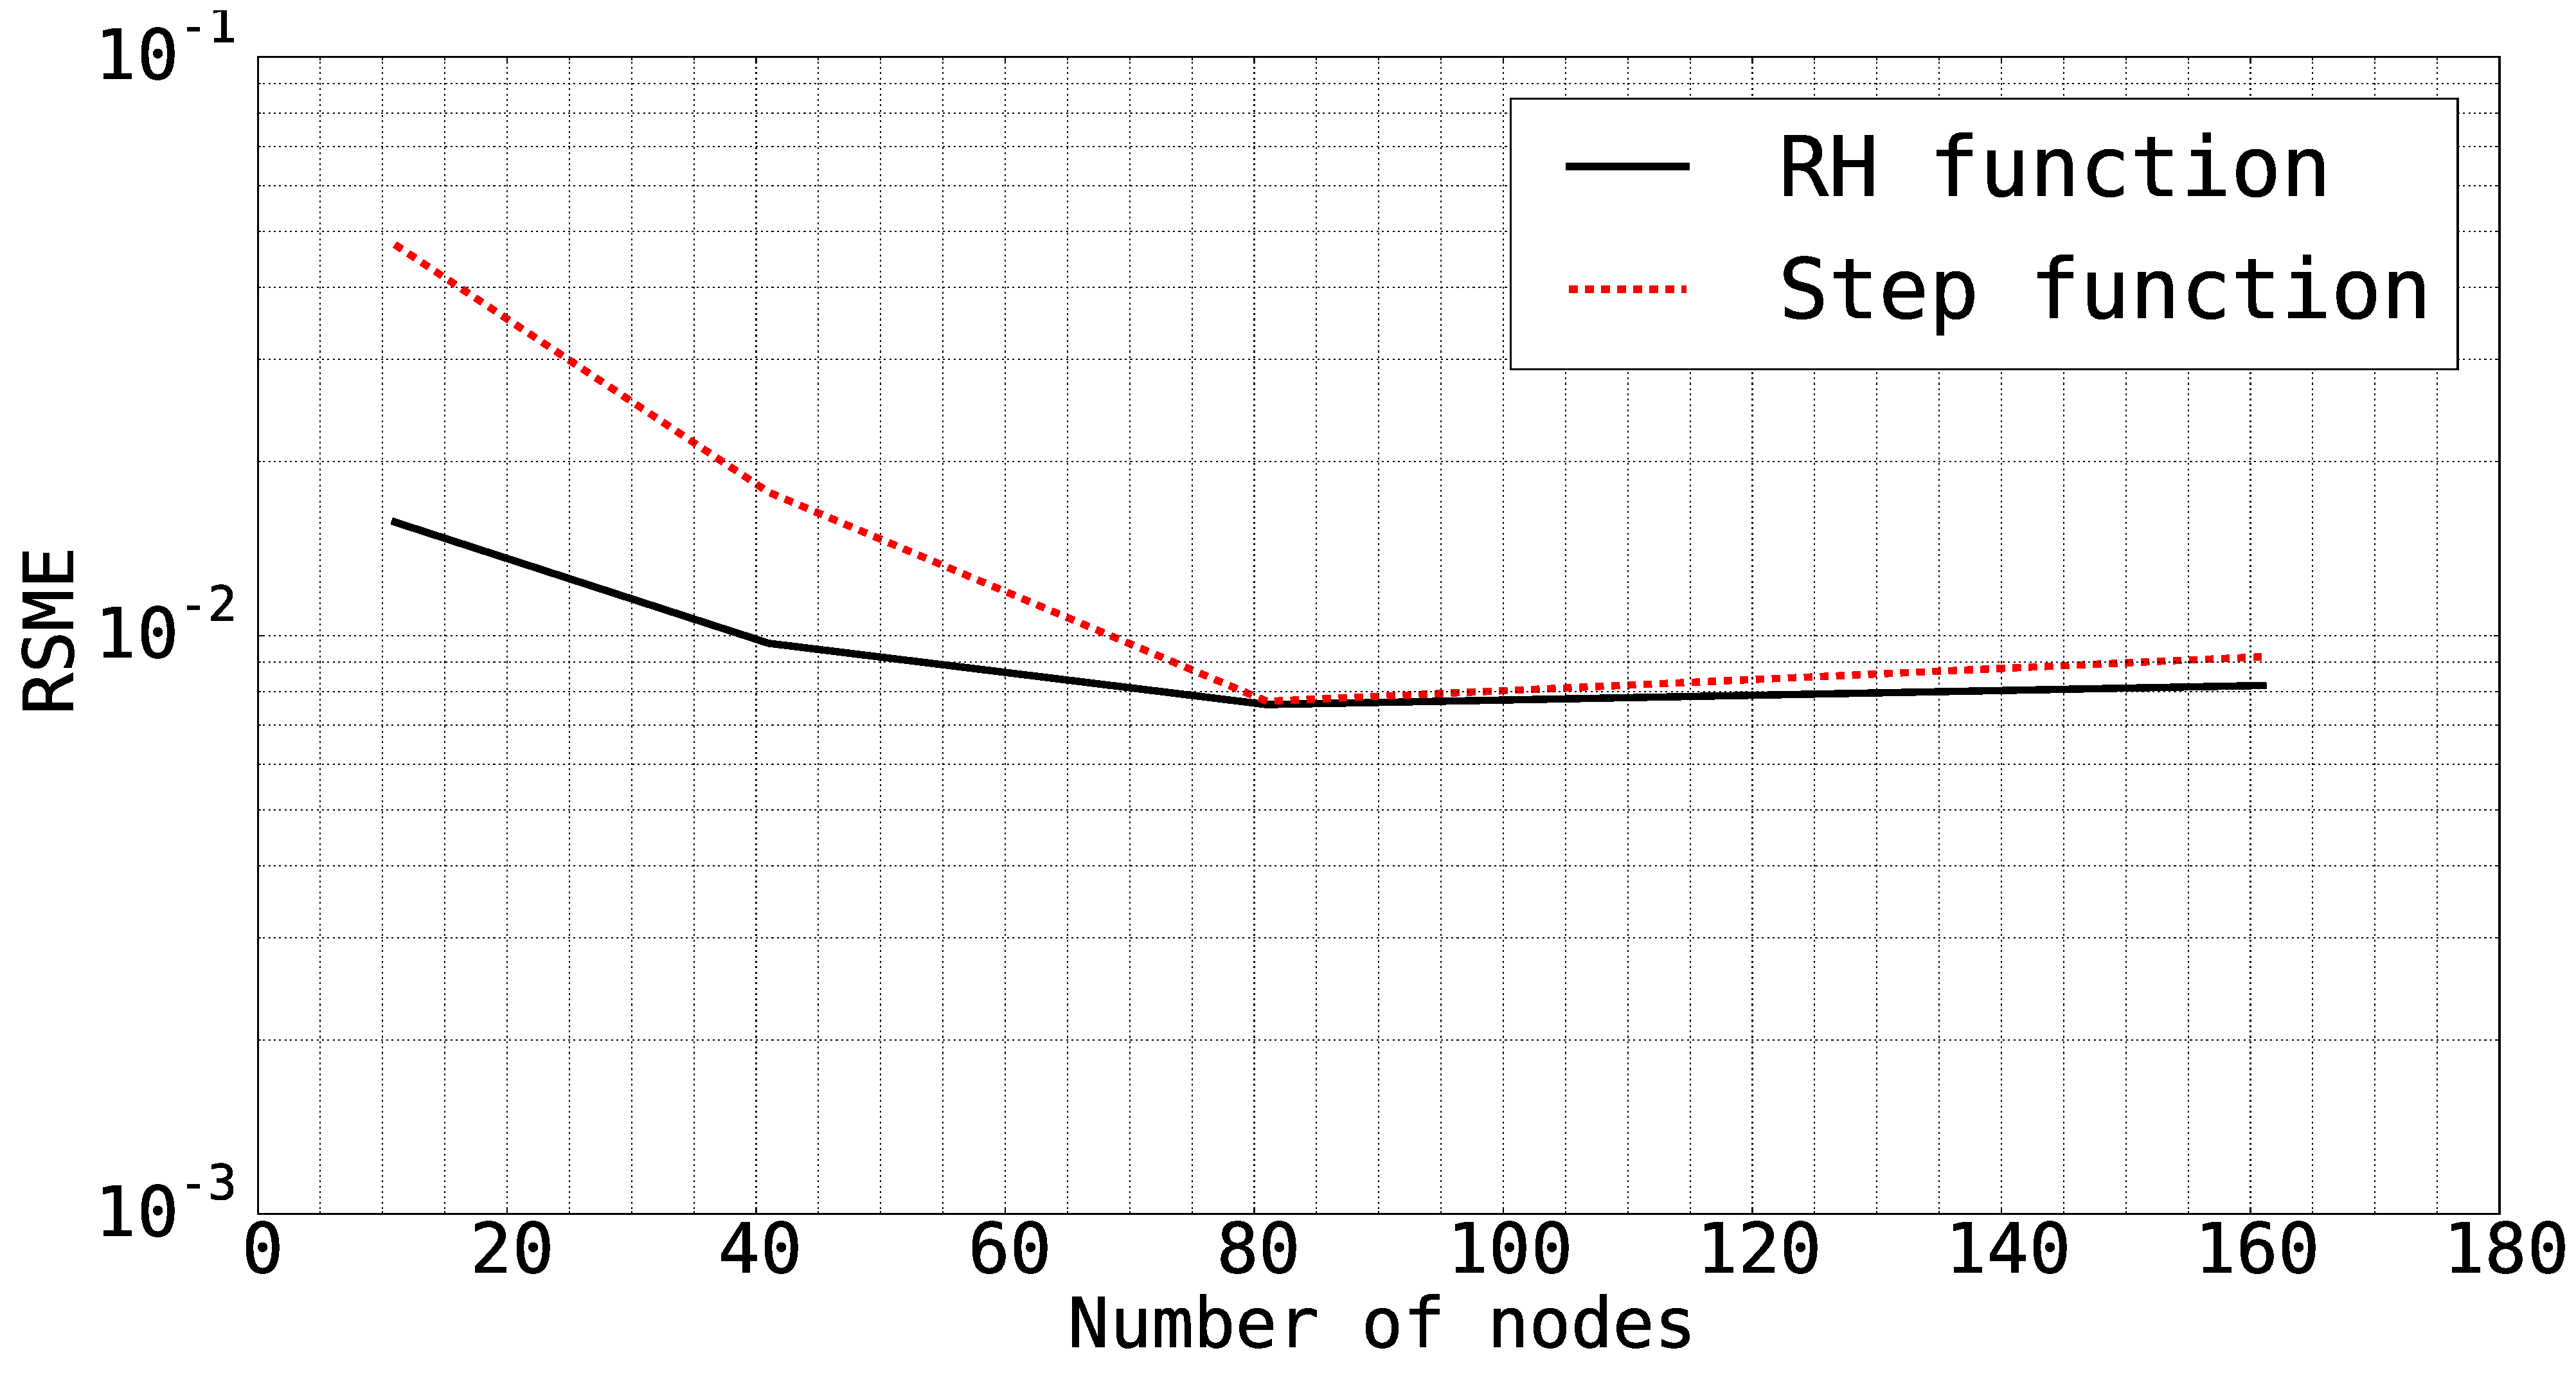
\includegraphics[width=12.00cm]{Chapter_4/figure/effect_of_RH_on_simulation_vs_numberOfNodes_1D_problem.eps}
	\caption{Effect of Regularized Heaviside (RH) and step function on the solution accuracy.}
	\label{fig:C4_effectOfRHfunctionOnSimulationResults1Dproblem}
\end{figure}

As shown in Figure \ref{fig:C4_effectOfRHfunctionOnSimulationResults1Dproblem}, the result of the RH function are more accurate compared to the step function. The effect of wall velocity of the accuracy of the simulation was also investigated. The wall velocity was selected as $1 m/s$, $10 m/s$, $100 m/s$, and $1000 m/s$. However, this did not affect the accuracy of the simulation.

The sensitivity equations for the penalization technique are derived by differentiating the governing equation as shown in Equation \eqref{eq:C4_NSwithPenalizationIBsensitivity}. However, for this problem the convective terms and pressure gradient drop out resulting in the sensitivity equation as shown in Equation \eqref{eq:C4_SAforPenlizationMethod1D}.

\begin{equation}\label{eq:C4_SAforPenlizationMethod1D}
	\frac{\partial u'}{\partial t} = 
	\mu \frac{\partial^2 u'}{\partial x^2} +
	\kappa \left[
	\frac{\partial \mathcal{H}}{\partial X} \frac{\partial X}{\partial b} + 
	\mathcal{H}(X) u'
	\right]
\end{equation}

where $X$ is $x - x_w$ and $x_w$ is the location of the solid wall. $u$ is the flow velocity, $\mu$ is the viscosity, $\kappa$ is the porosity, and $\mathcal{H}$ is the RH function. $b$ corresponds to the generic design variable and $u'$ is the sensitivity of the flow field to the design variable $b$. The boundary conditions are derived by differentiating the Equation \eqref{eq:C4_1DbenchmarkBoundaryCondition}. This is shown in Equation \eqref{eq:C4_SAboundaryConditionforPenlizationMethod1D}. Both of the boundary conditions are zero because their location does not change by changing the design variable.

\begin{equation}\label{eq:C4_SAboundaryConditionforPenlizationMethod1D}
\begin{cases}
	u' = 0 \qquad \text{at } x = 0 \\
	u' = 0 \quad \text{at } x = 1
\end{cases}
\end{equation}

For this problem, the $\kappa$ is selected as $2 \time 10^4$ based on the convergence studies for the governing equations and the sensitivity of the velocity profile with respect to the distance between two plates is verified with Equation \eqref{eq:C4_1DbenchmarkAnalyticalSAlength}. The $\eta$ parameter for the RH function is selected in such a way that 95 percent of change in RH function occurs within two nodes from the solid boundary. This ensures the stability of the method. The initial location of wall is selected as $x_{wall} = 0.4321$ and $x_{wall} = 0.7583$. Neither of these locations coincide with the computational nodes in the domain. The effect of number of nodes on the accuracy of the solution of the governign equations and the sensitivity results are shown in Figure \ref{fig:C4_effectOfNumberOfNodesOnSensitivityResults1Dproblem}.

\begin{figure}[H]
    \centering
    \subfigure[$x_{wall} = 0.4321$]
    {
    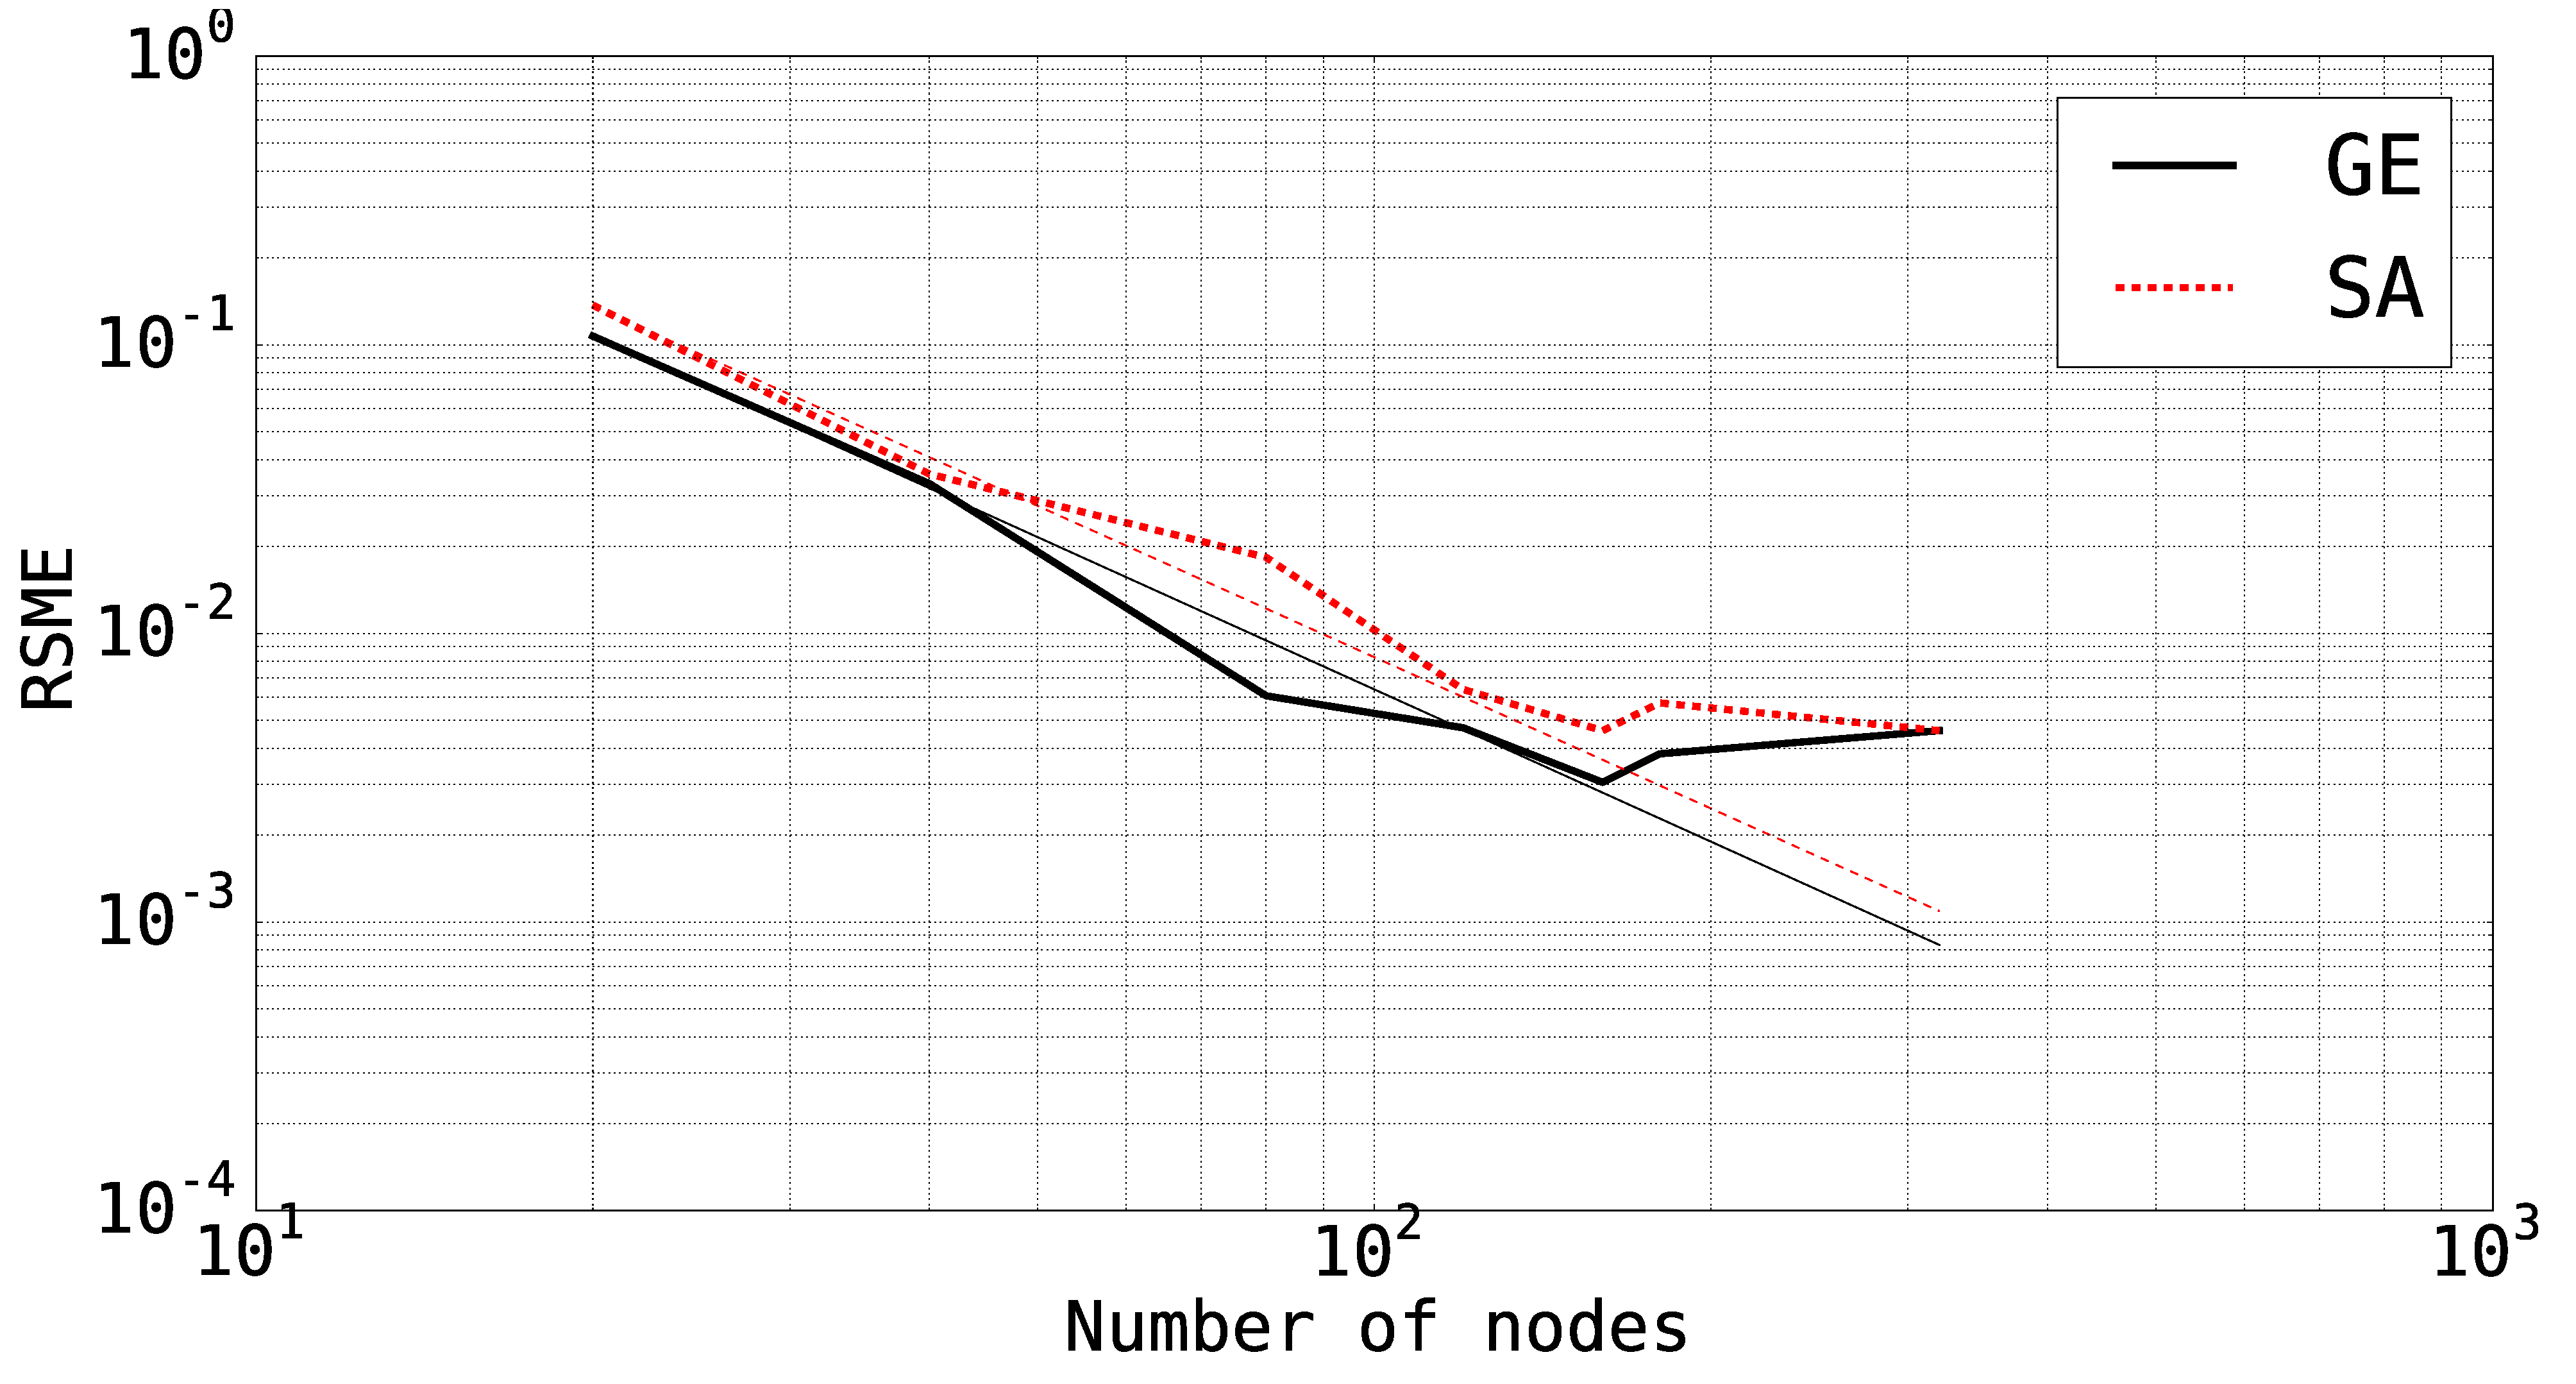
\includegraphics[width=12.0cm]{Chapter_4/figure/penalizationMethod_SA_1D_problem_xw04321.eps}
    }
    \\
    \subfigure[$x_{wall} = 0.7583$]
    {
    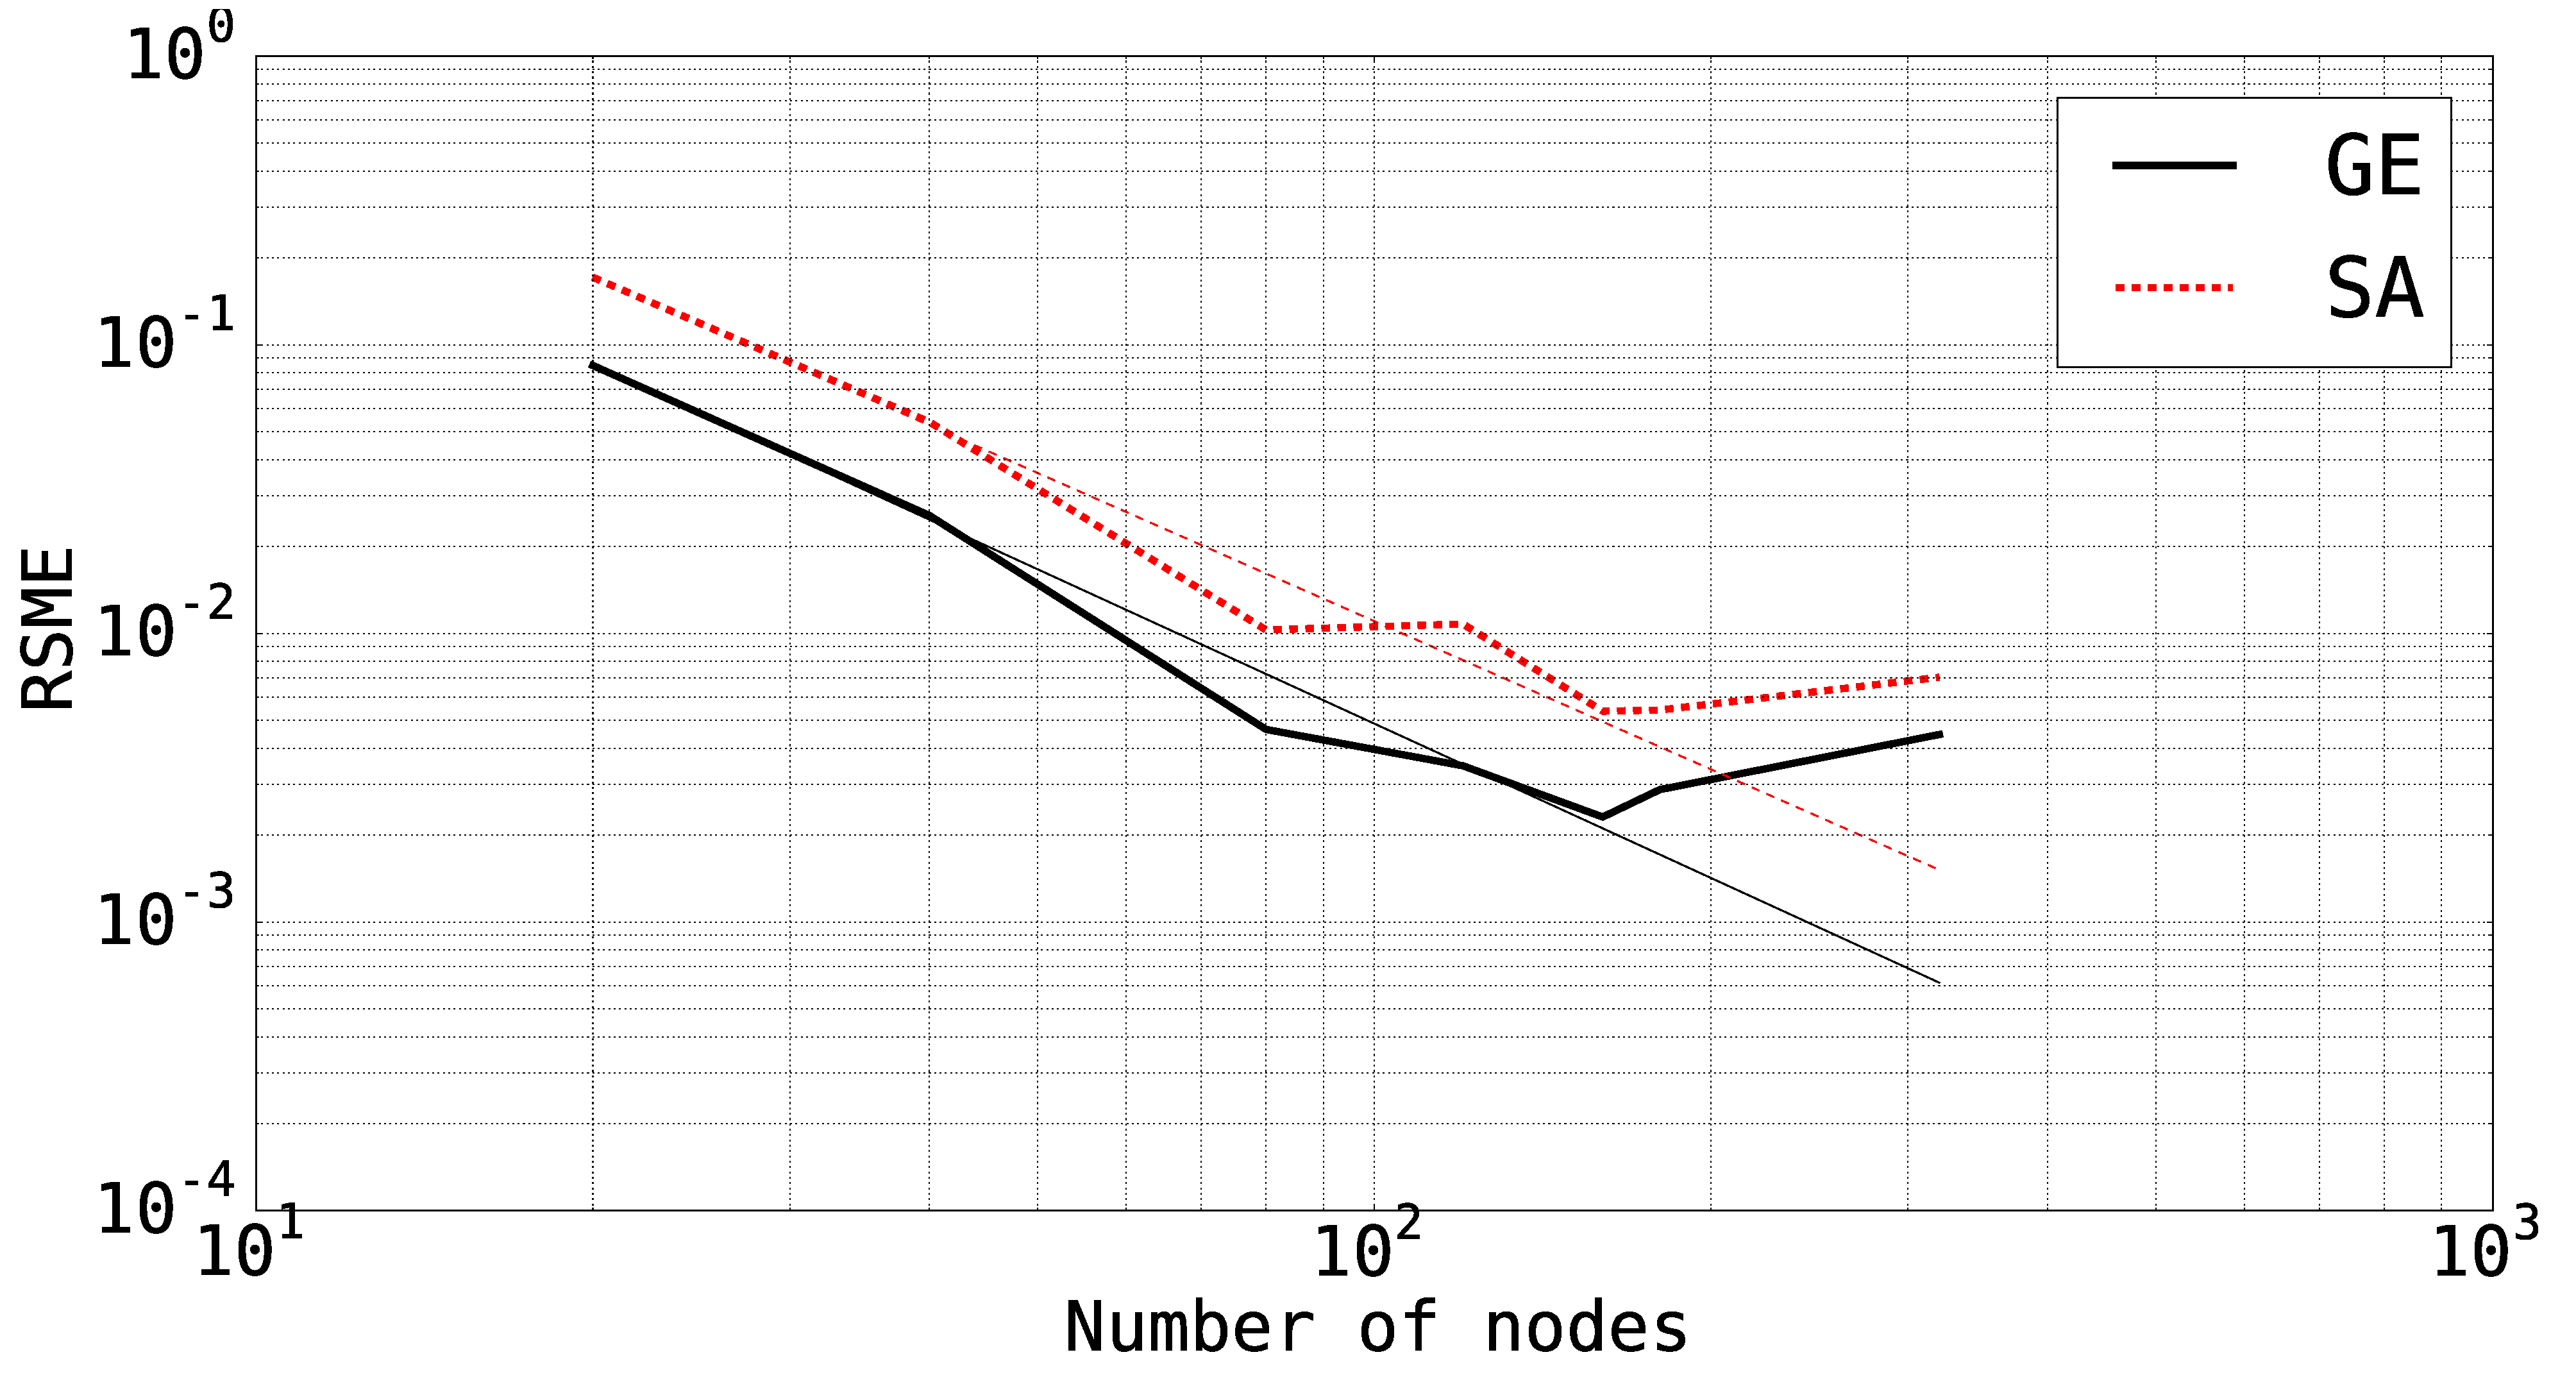
\includegraphics[width=12.0cm]{Chapter_4/figure/penalizationMethod_SA_1D_problem_xw07583.eps}
    }
    \caption{RSME value for the sensitivity analysis (SA) and governing equation (GE).}
    \label{fig:C4_effectOfNumberOfNodesOnSensitivityResults1Dproblem}
\end{figure}

The thin lines in Figure \ref{fig:C4_effectOfRHfunctionOnSimulationResults1Dproblem}, represents the curve fit by function $y = ae^{bx}$ through the RSME values. The slope of this line is $-1.75$ for both of these analysis. This means that the rate of convergence is the same for governing equations and sensitivity analysis for this problem. The source of the error between the analytical and the CSA is better investigated by looking at the comparison between the sensitivity of the velocity profile to the distance between the plates as shown in Figure \ref{fig:C4_sensitivityResults1Dproblem}.

\begin{figure}[H]
    \centering
    \subfigure[$x_{wall} = 0.4321, n = 120$]
    {
    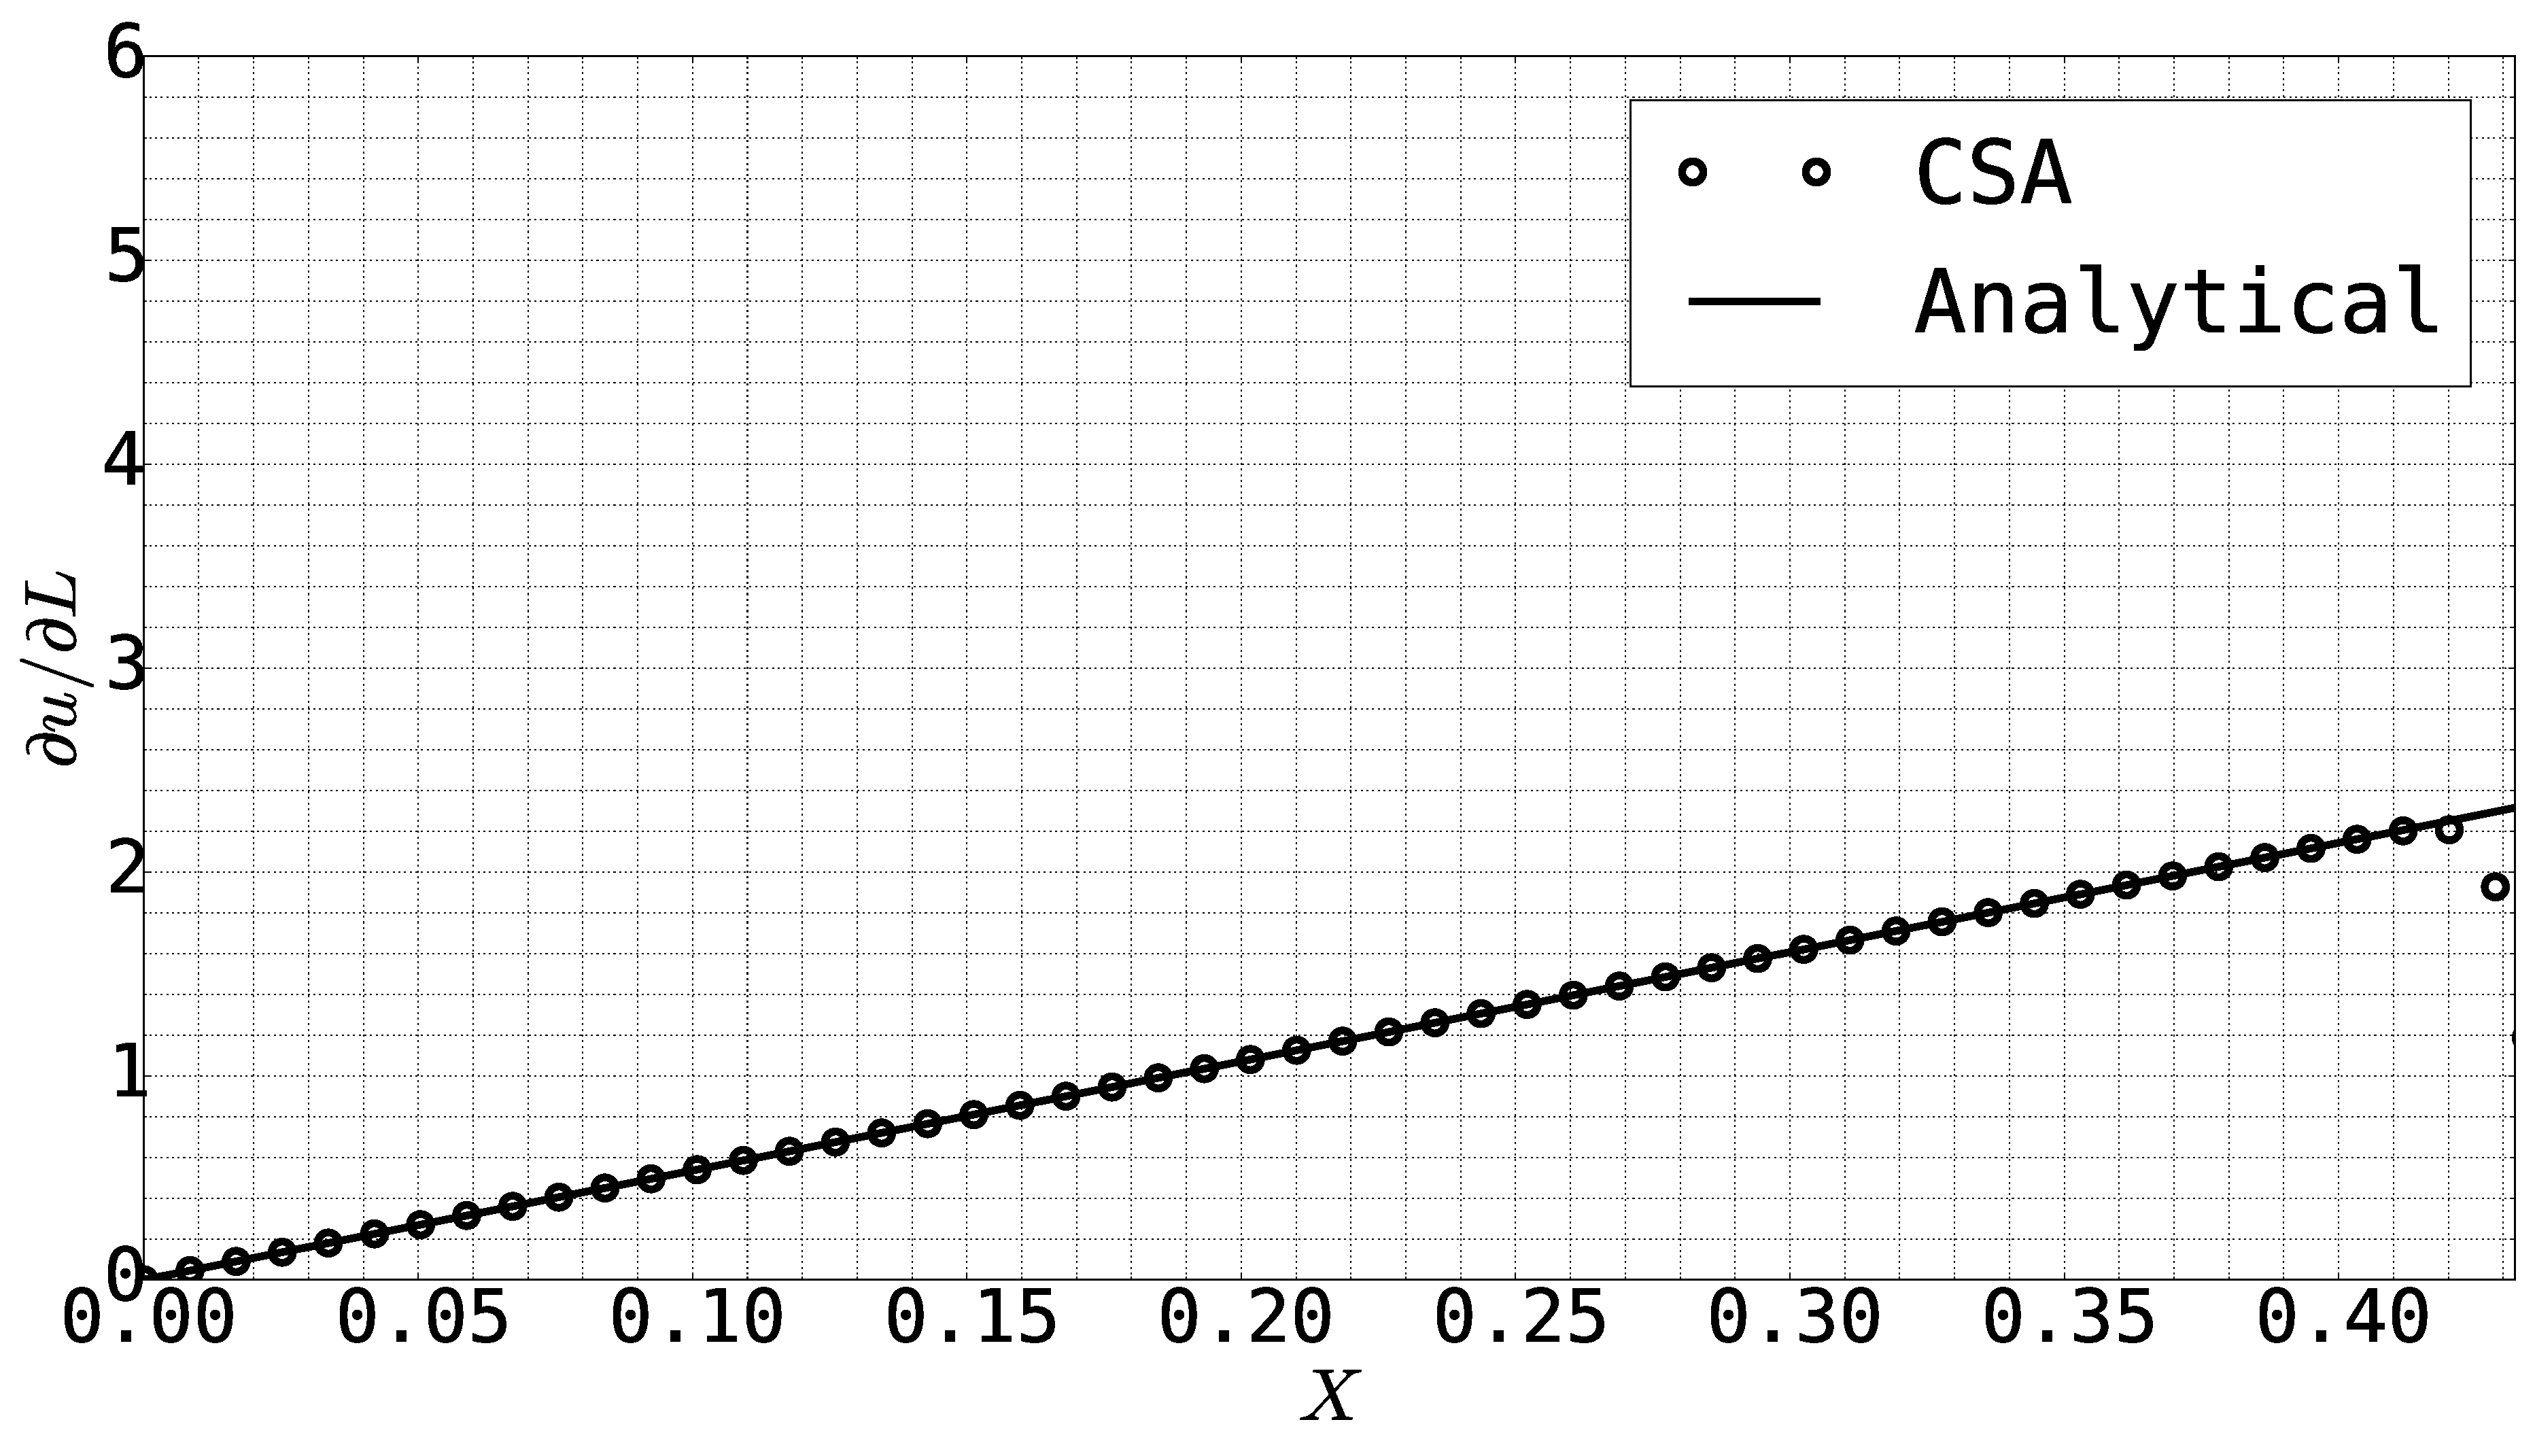
\includegraphics[width=7.0cm]{Chapter_4/figure/penalizationMethod_sensitivityProfile_xw04321.eps}
    }
    \quad
    \subfigure[$x_{wall} = 0.7583, n = 120$]
    {
    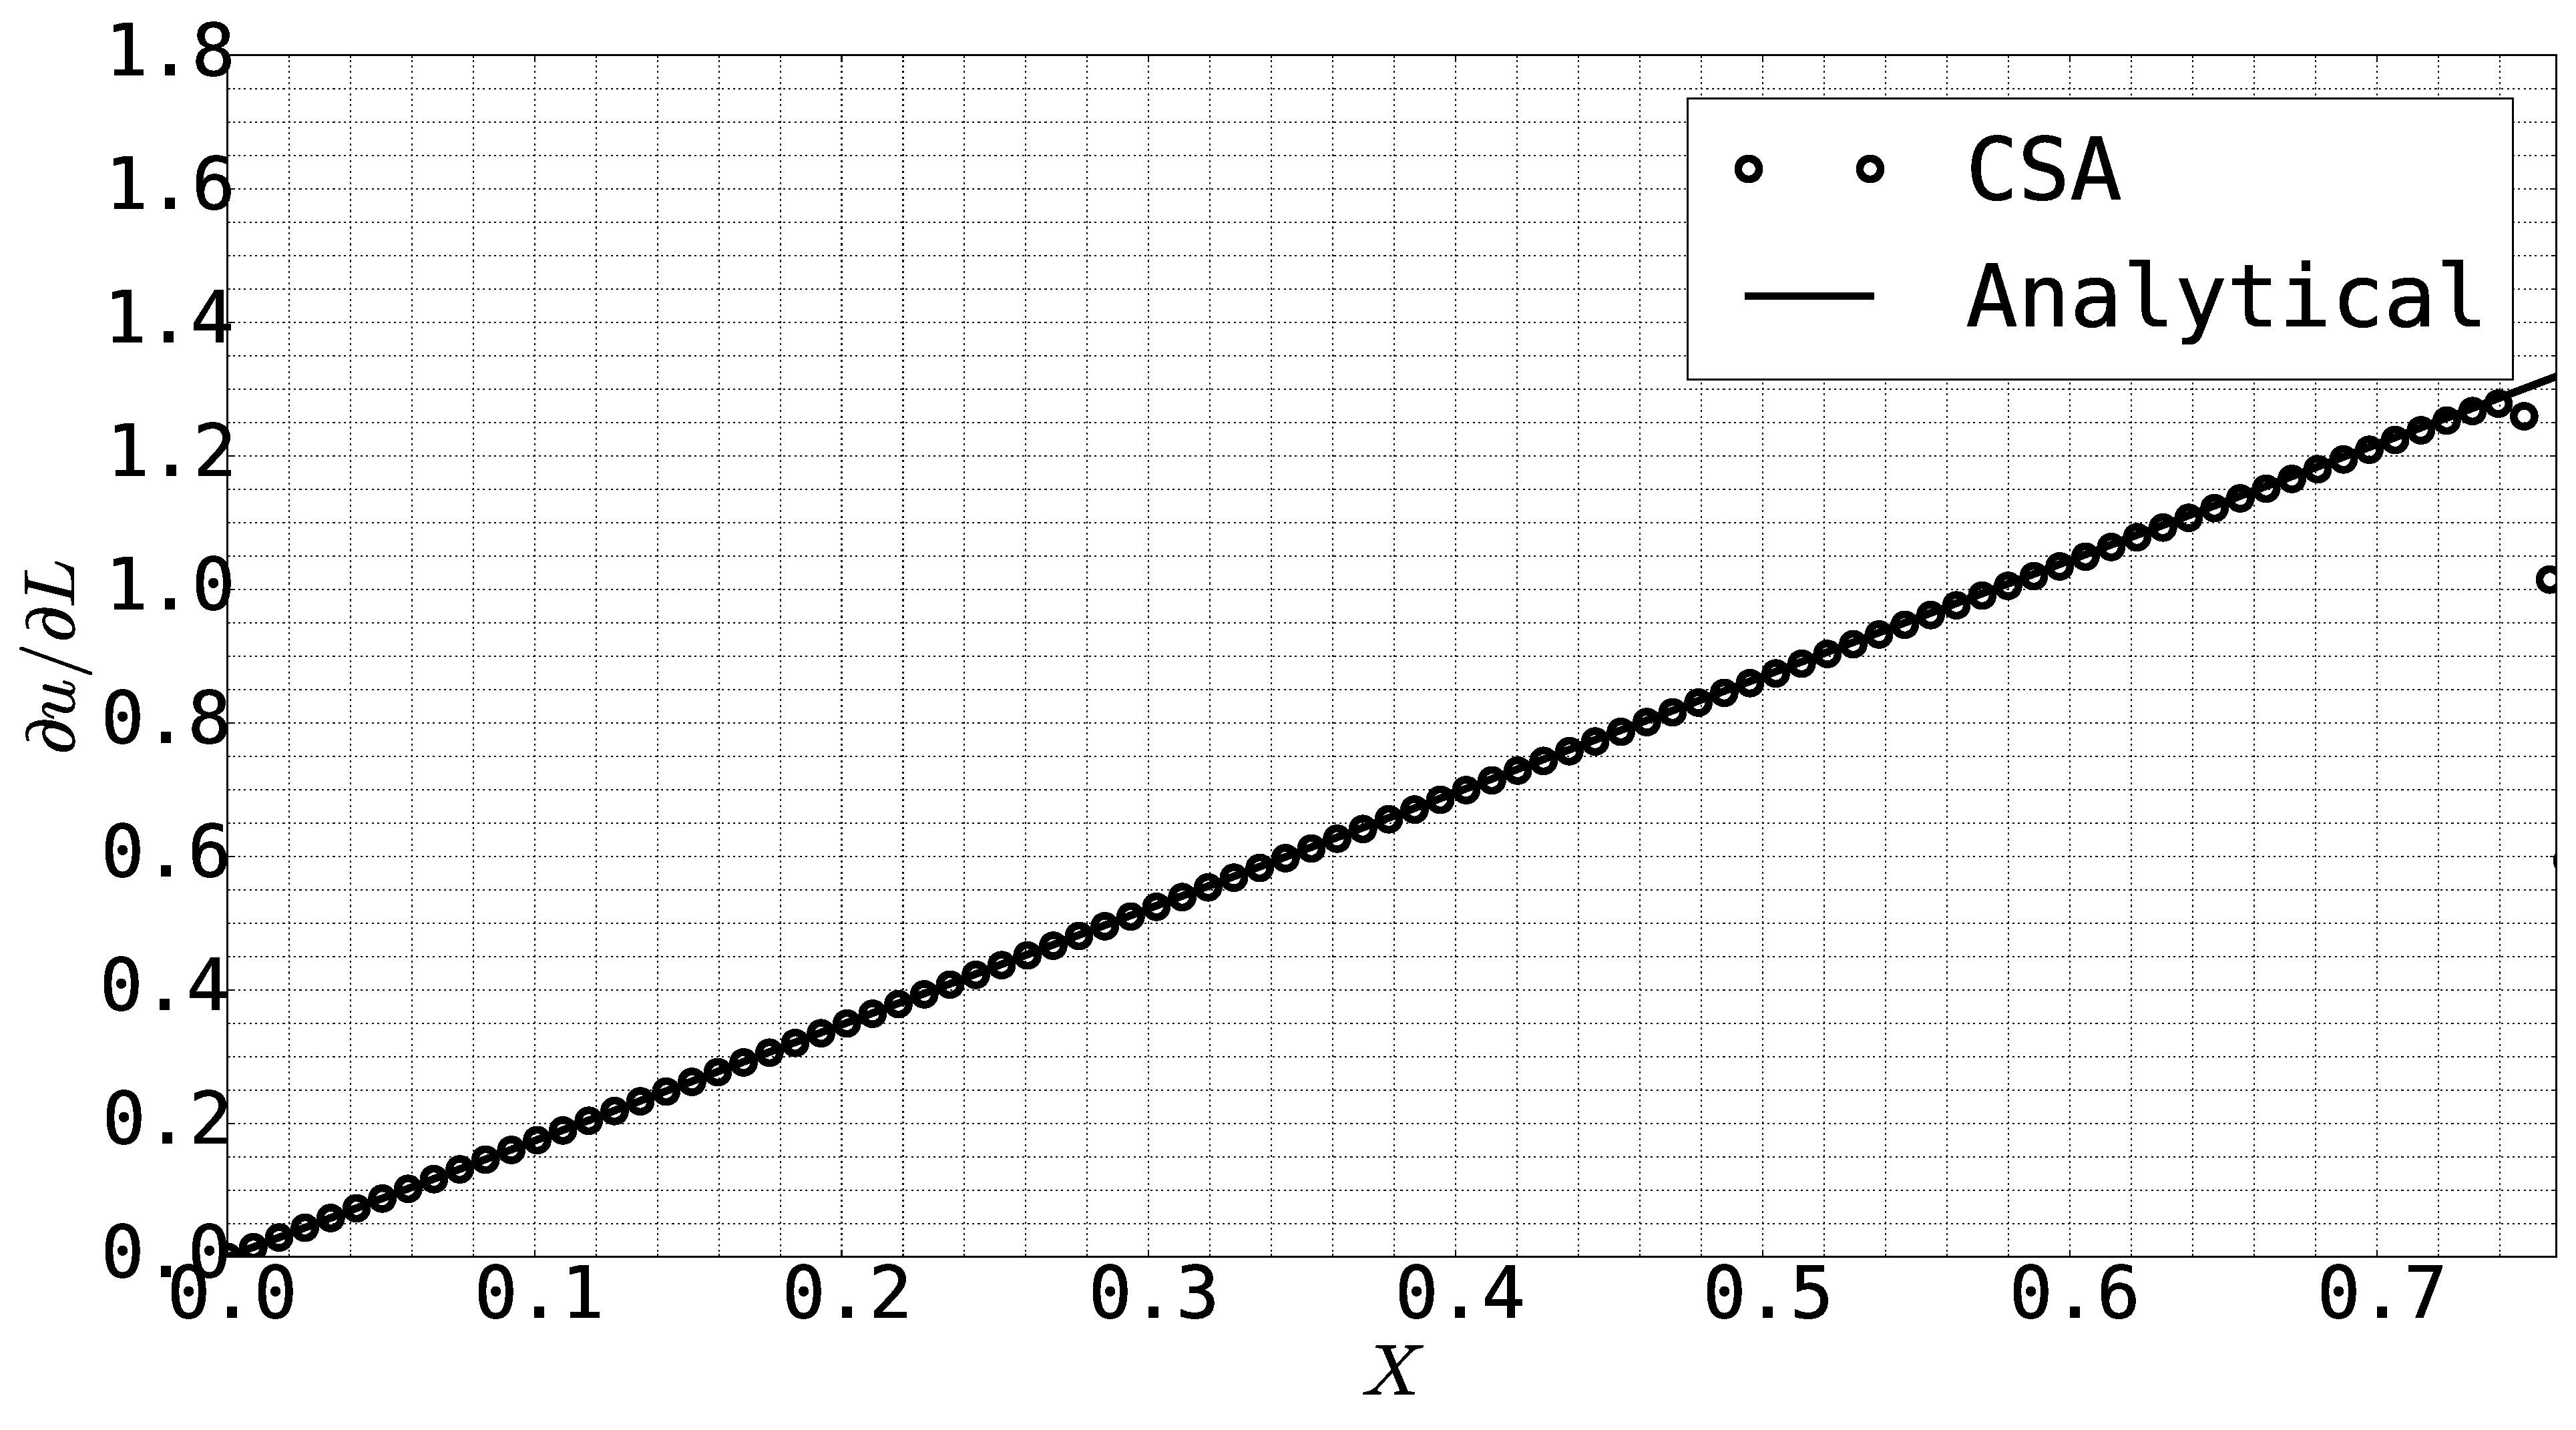
\includegraphics[width=7.0cm]{Chapter_4/figure/penalizationMethod_sensitivityProfile_xw07583.eps}
    }
    \\
    \subfigure[$x_{wall} = 0.2451, n = 30$]
    {
    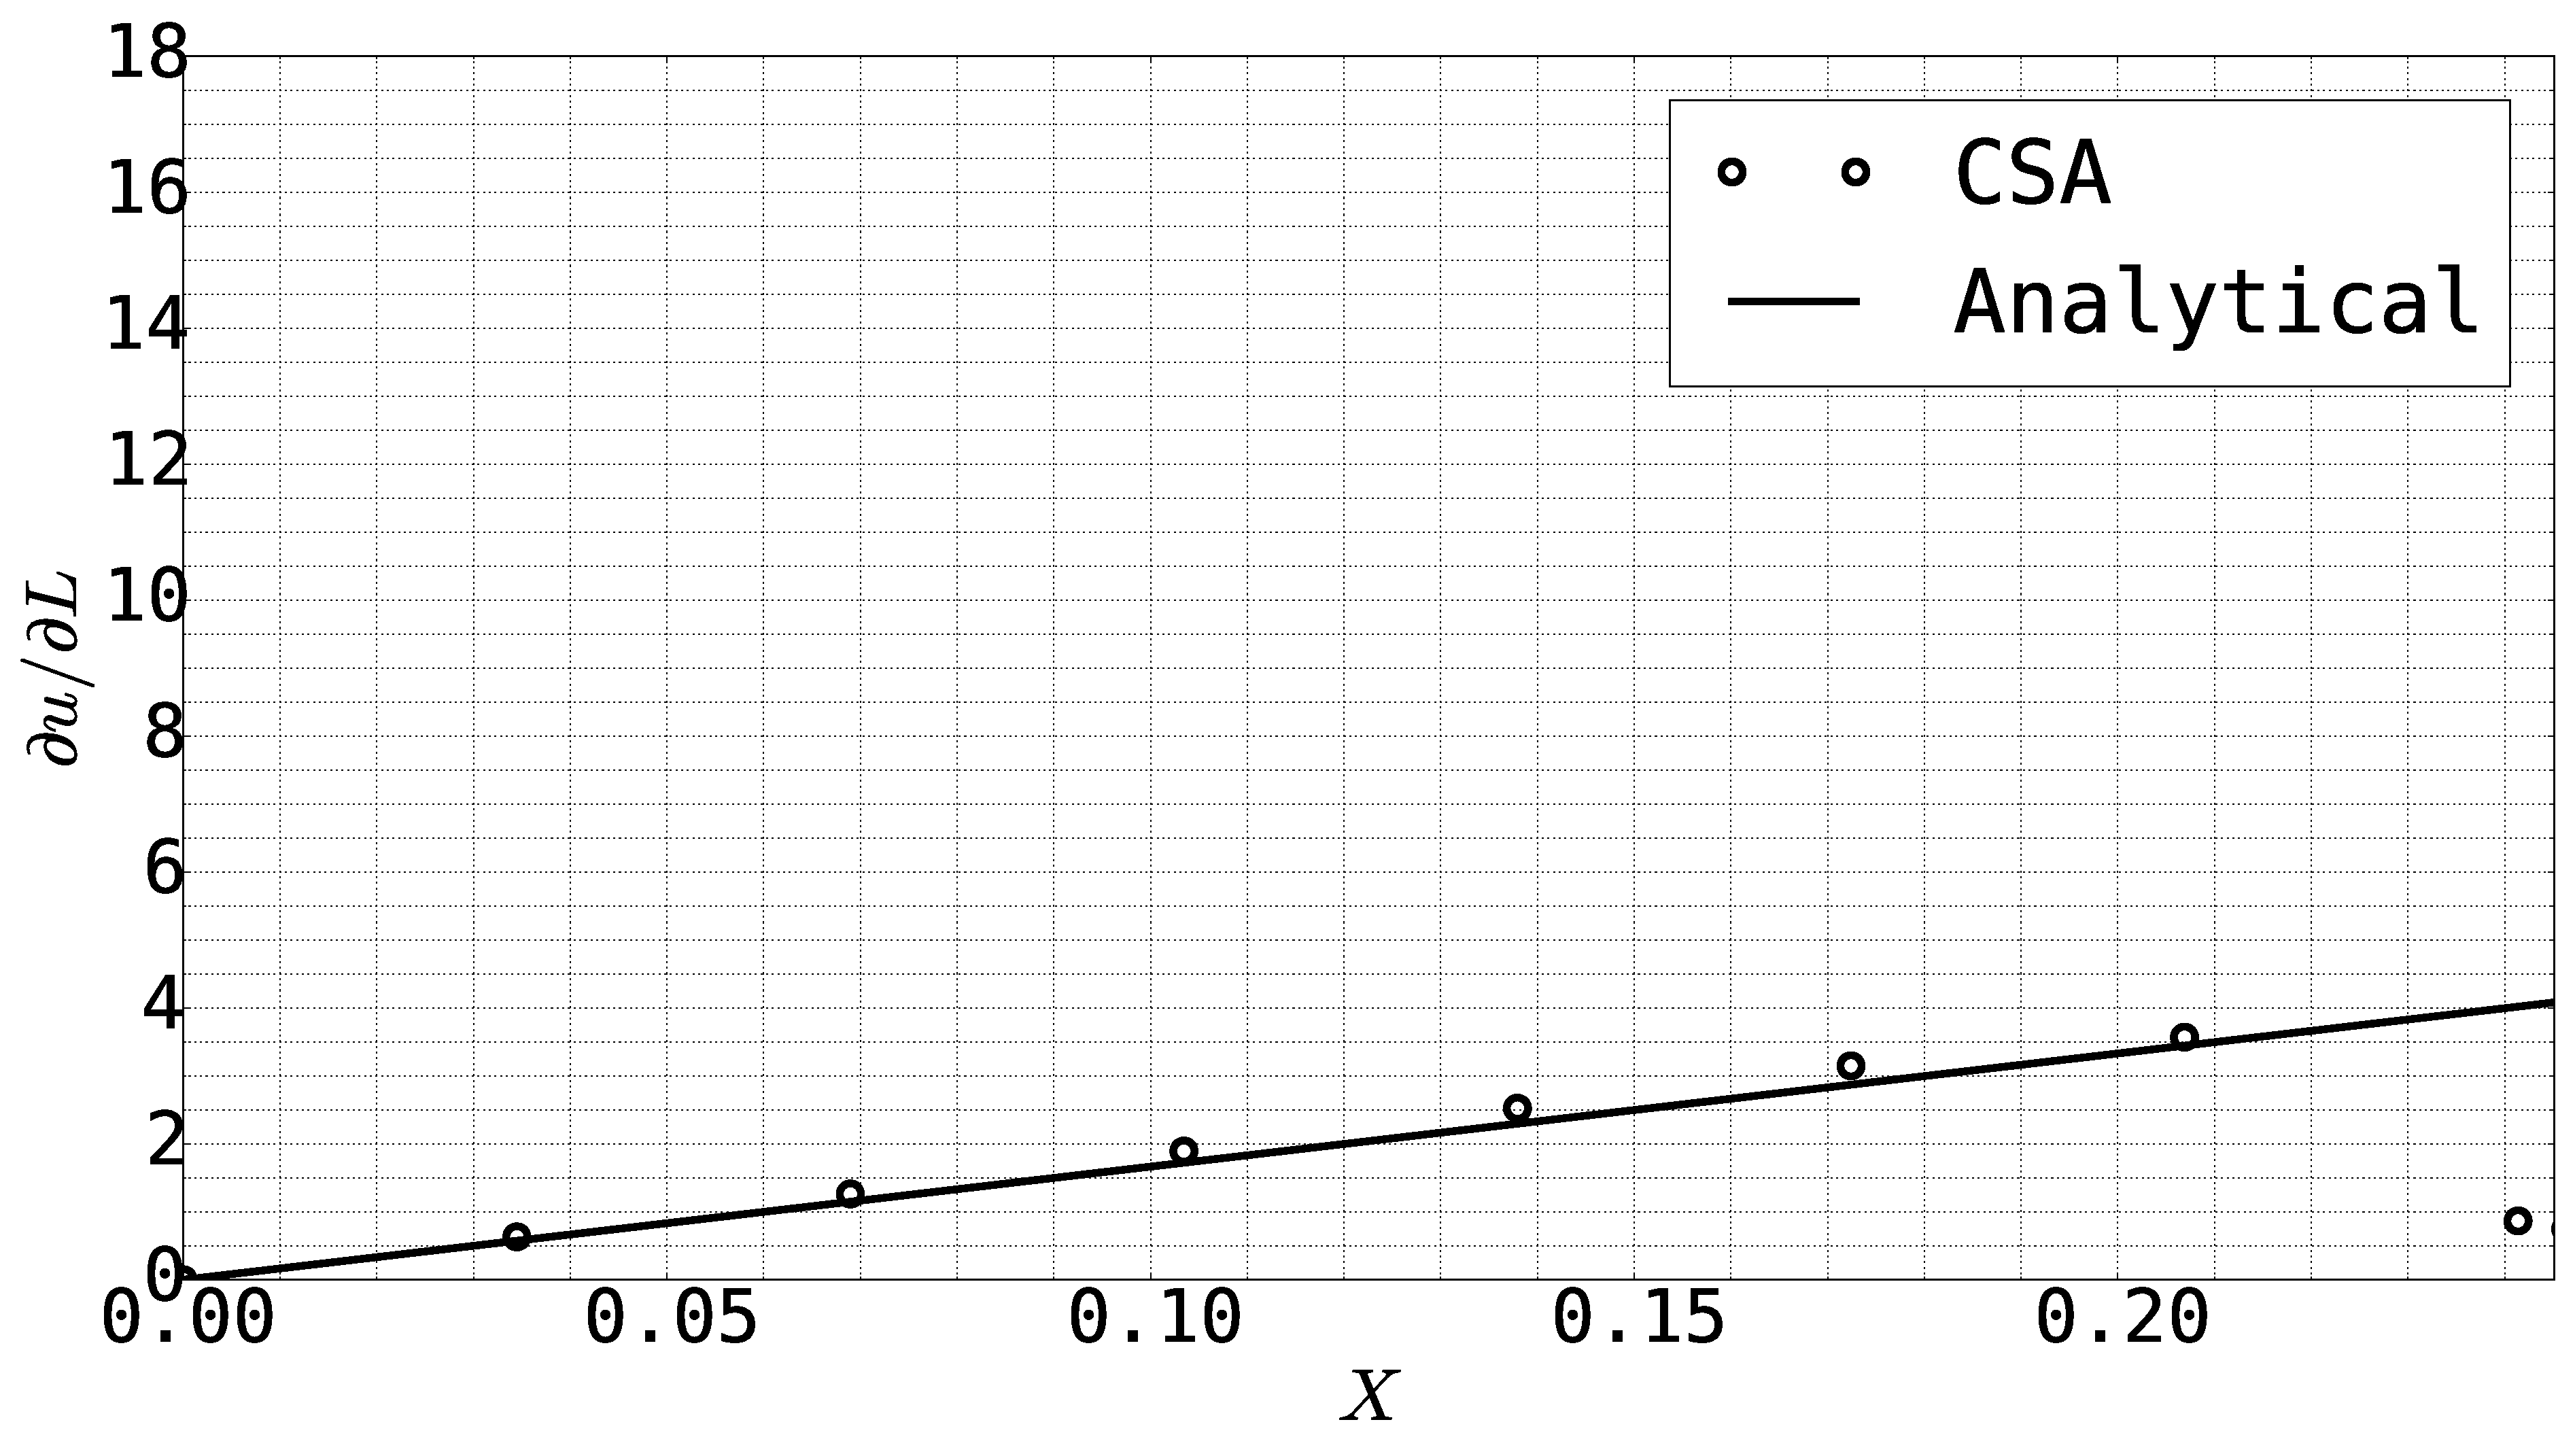
\includegraphics[width=7.0cm]{Chapter_4/figure/penalizationMethod_sensitivityProfile_xw02451.eps}
    }
    \quad
    \subfigure[$x_{wall} = 0.5742, n = 60$]
    {
    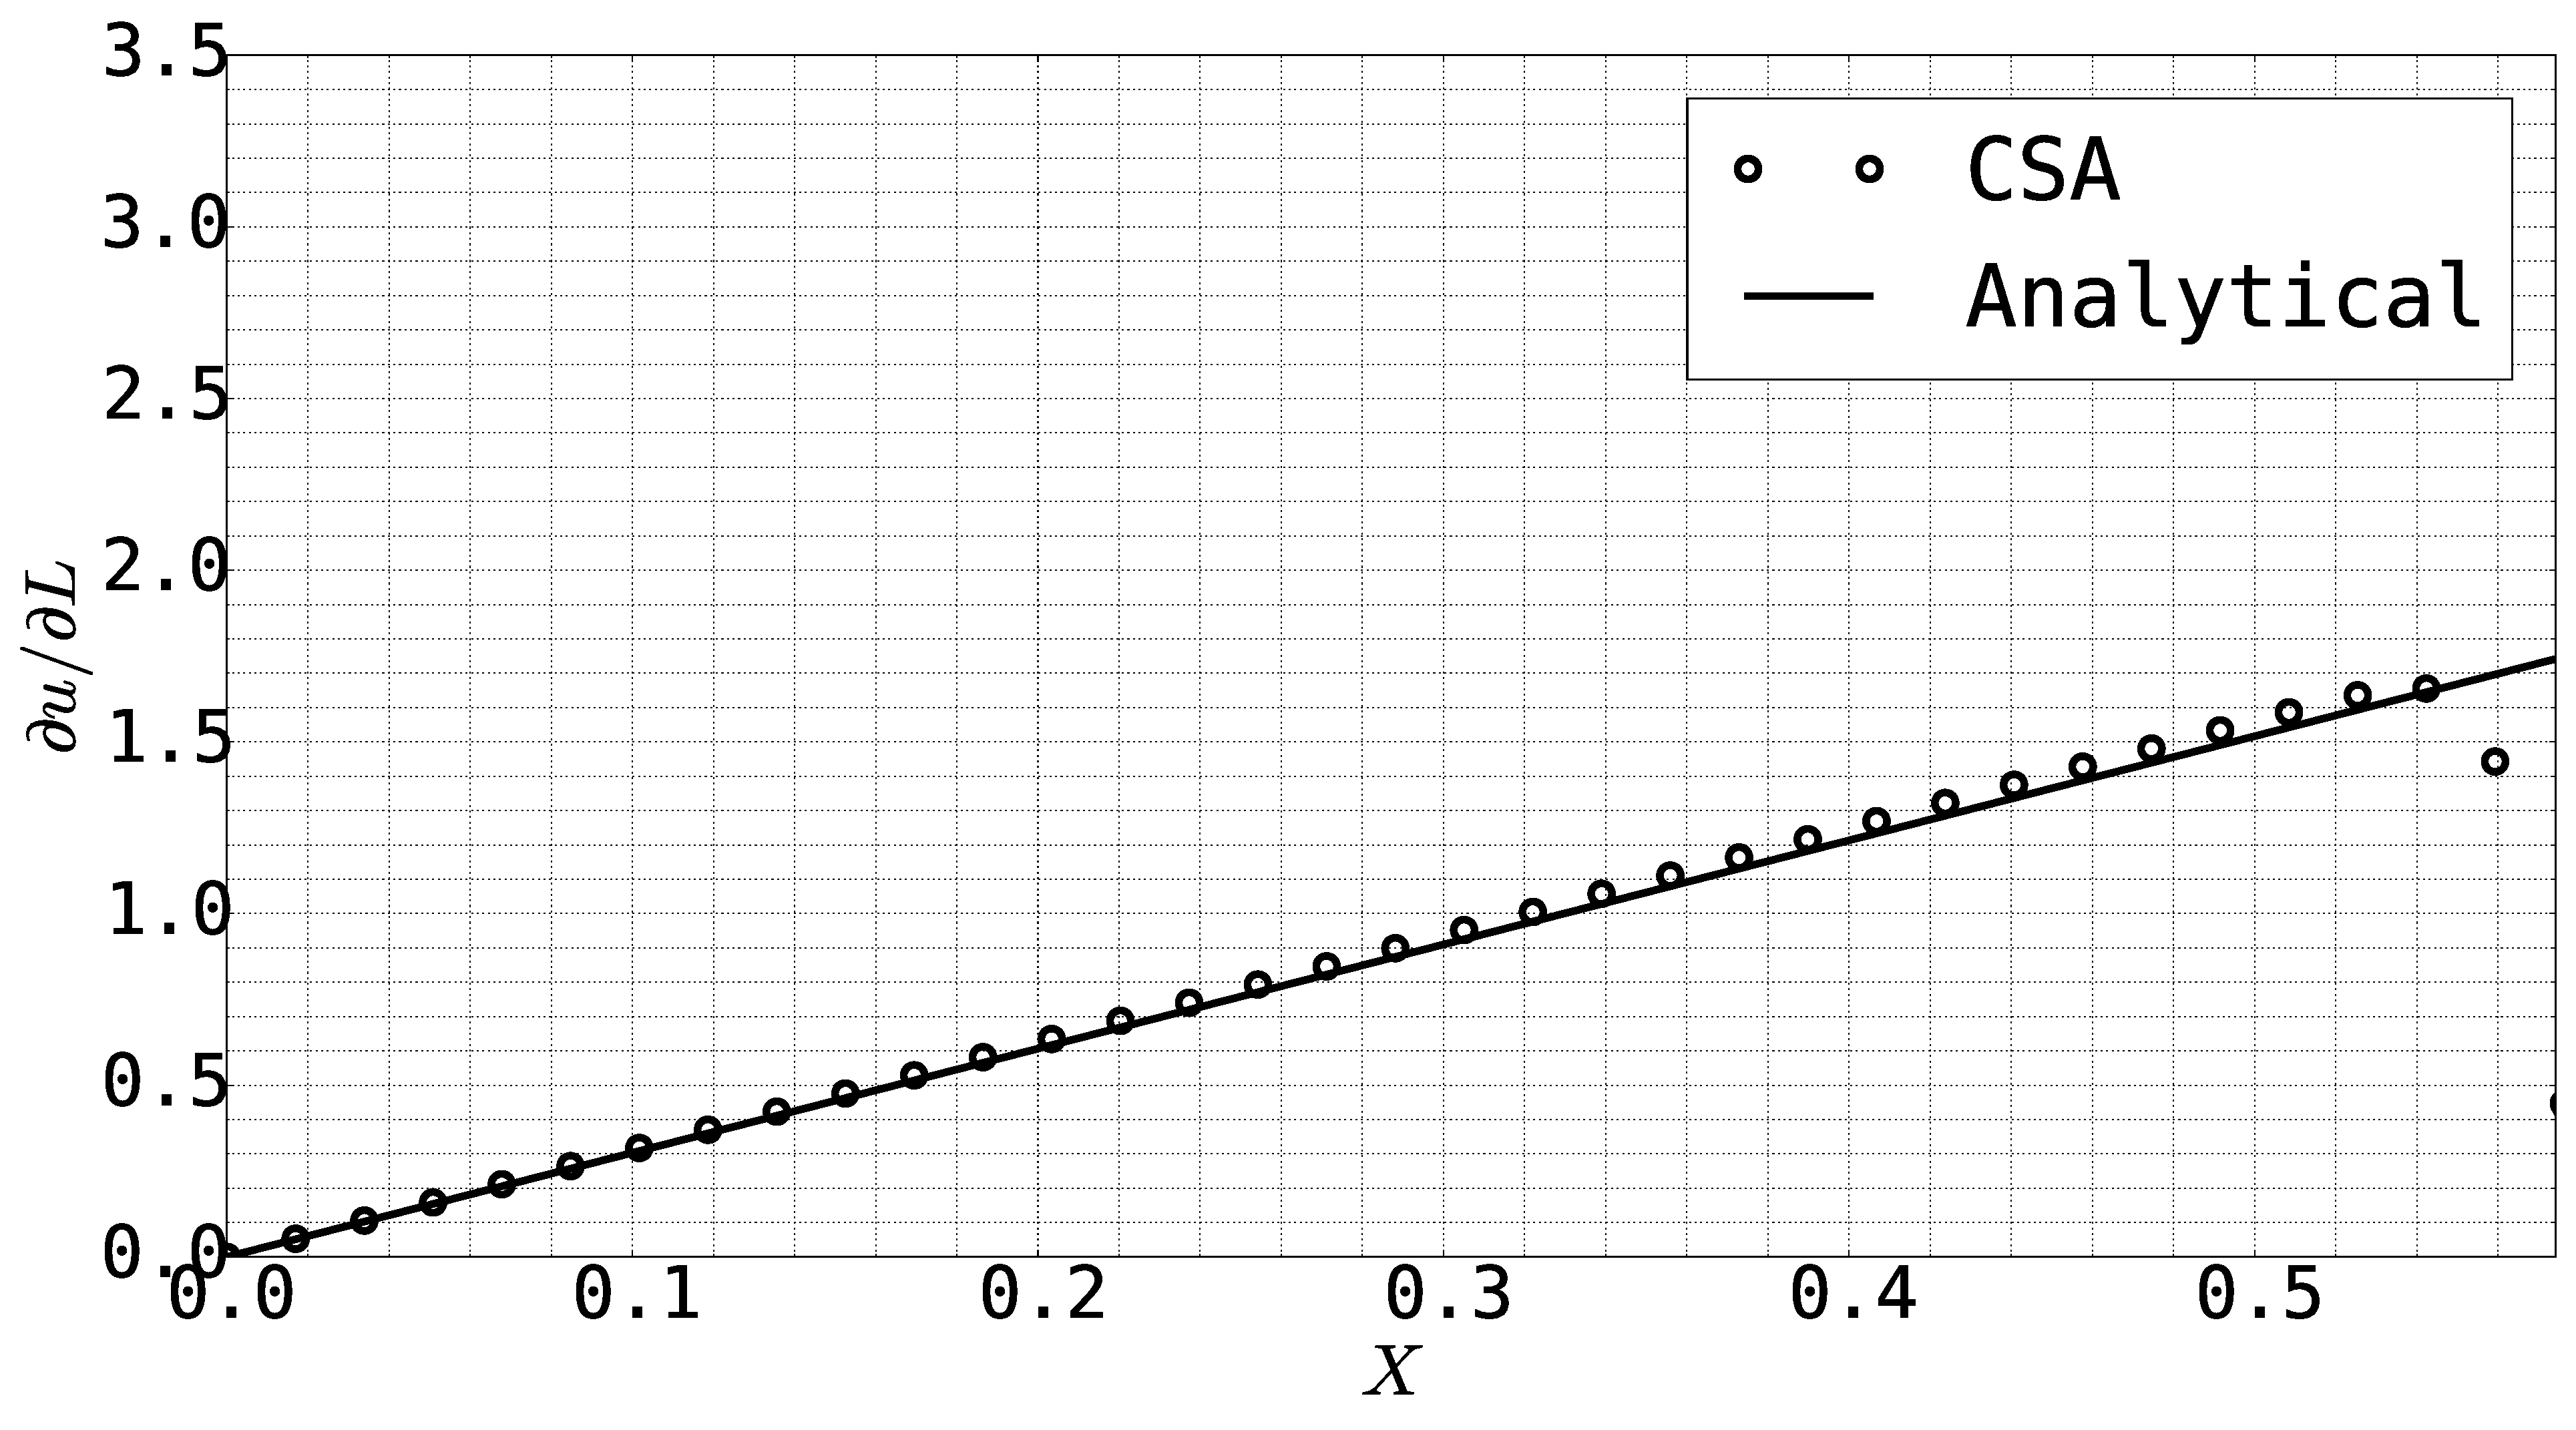
\includegraphics[width=7.0cm]{Chapter_4/figure/penalizationMethod_sensitivityProfile_xw05742.eps}
    }
    \caption{Comparison between the velocity sensitivity profile of CSA and analytical results in the domain. $w_{wall}$ is the location of the stationary wall and $n$ is the number of nodes used to discretize the domain.}
    \label{fig:C4_sensitivityResults1Dproblem}
\end{figure}

As shown in Figure \ref{fig:C4_sensitivityResults1Dproblem}, the accuracy of CSA results start to decay near the boundary. It should be noted that this domain corresponds to the region that we chose the RH function value to have its 99 percent change in. Therefore, the size of this region is known before the analysis. As shown in Figure \ref{fig:C4_sensitivityResults1Dproblem}, did not affect the sensitivity results in regions further away from the boundary. This means that the sensitivities near the boundary can be reconstructed by post-processing the sensitivity data. This is done using function approximation techniques such as linear extrapolation or TANA \cite{wang1995improved}. The reconstructed results of Figure \ref{fig:C4_sensitivityResults1Dproblem} using linear extrapolation are shown in Figure \ref{fig:C4_sensitivityResultsReconstructed1Dproblem}.

\begin{figure}[H]
    \centering
    \subfigure[$x_{wall} = 0.4321, n = 120$]
    {
    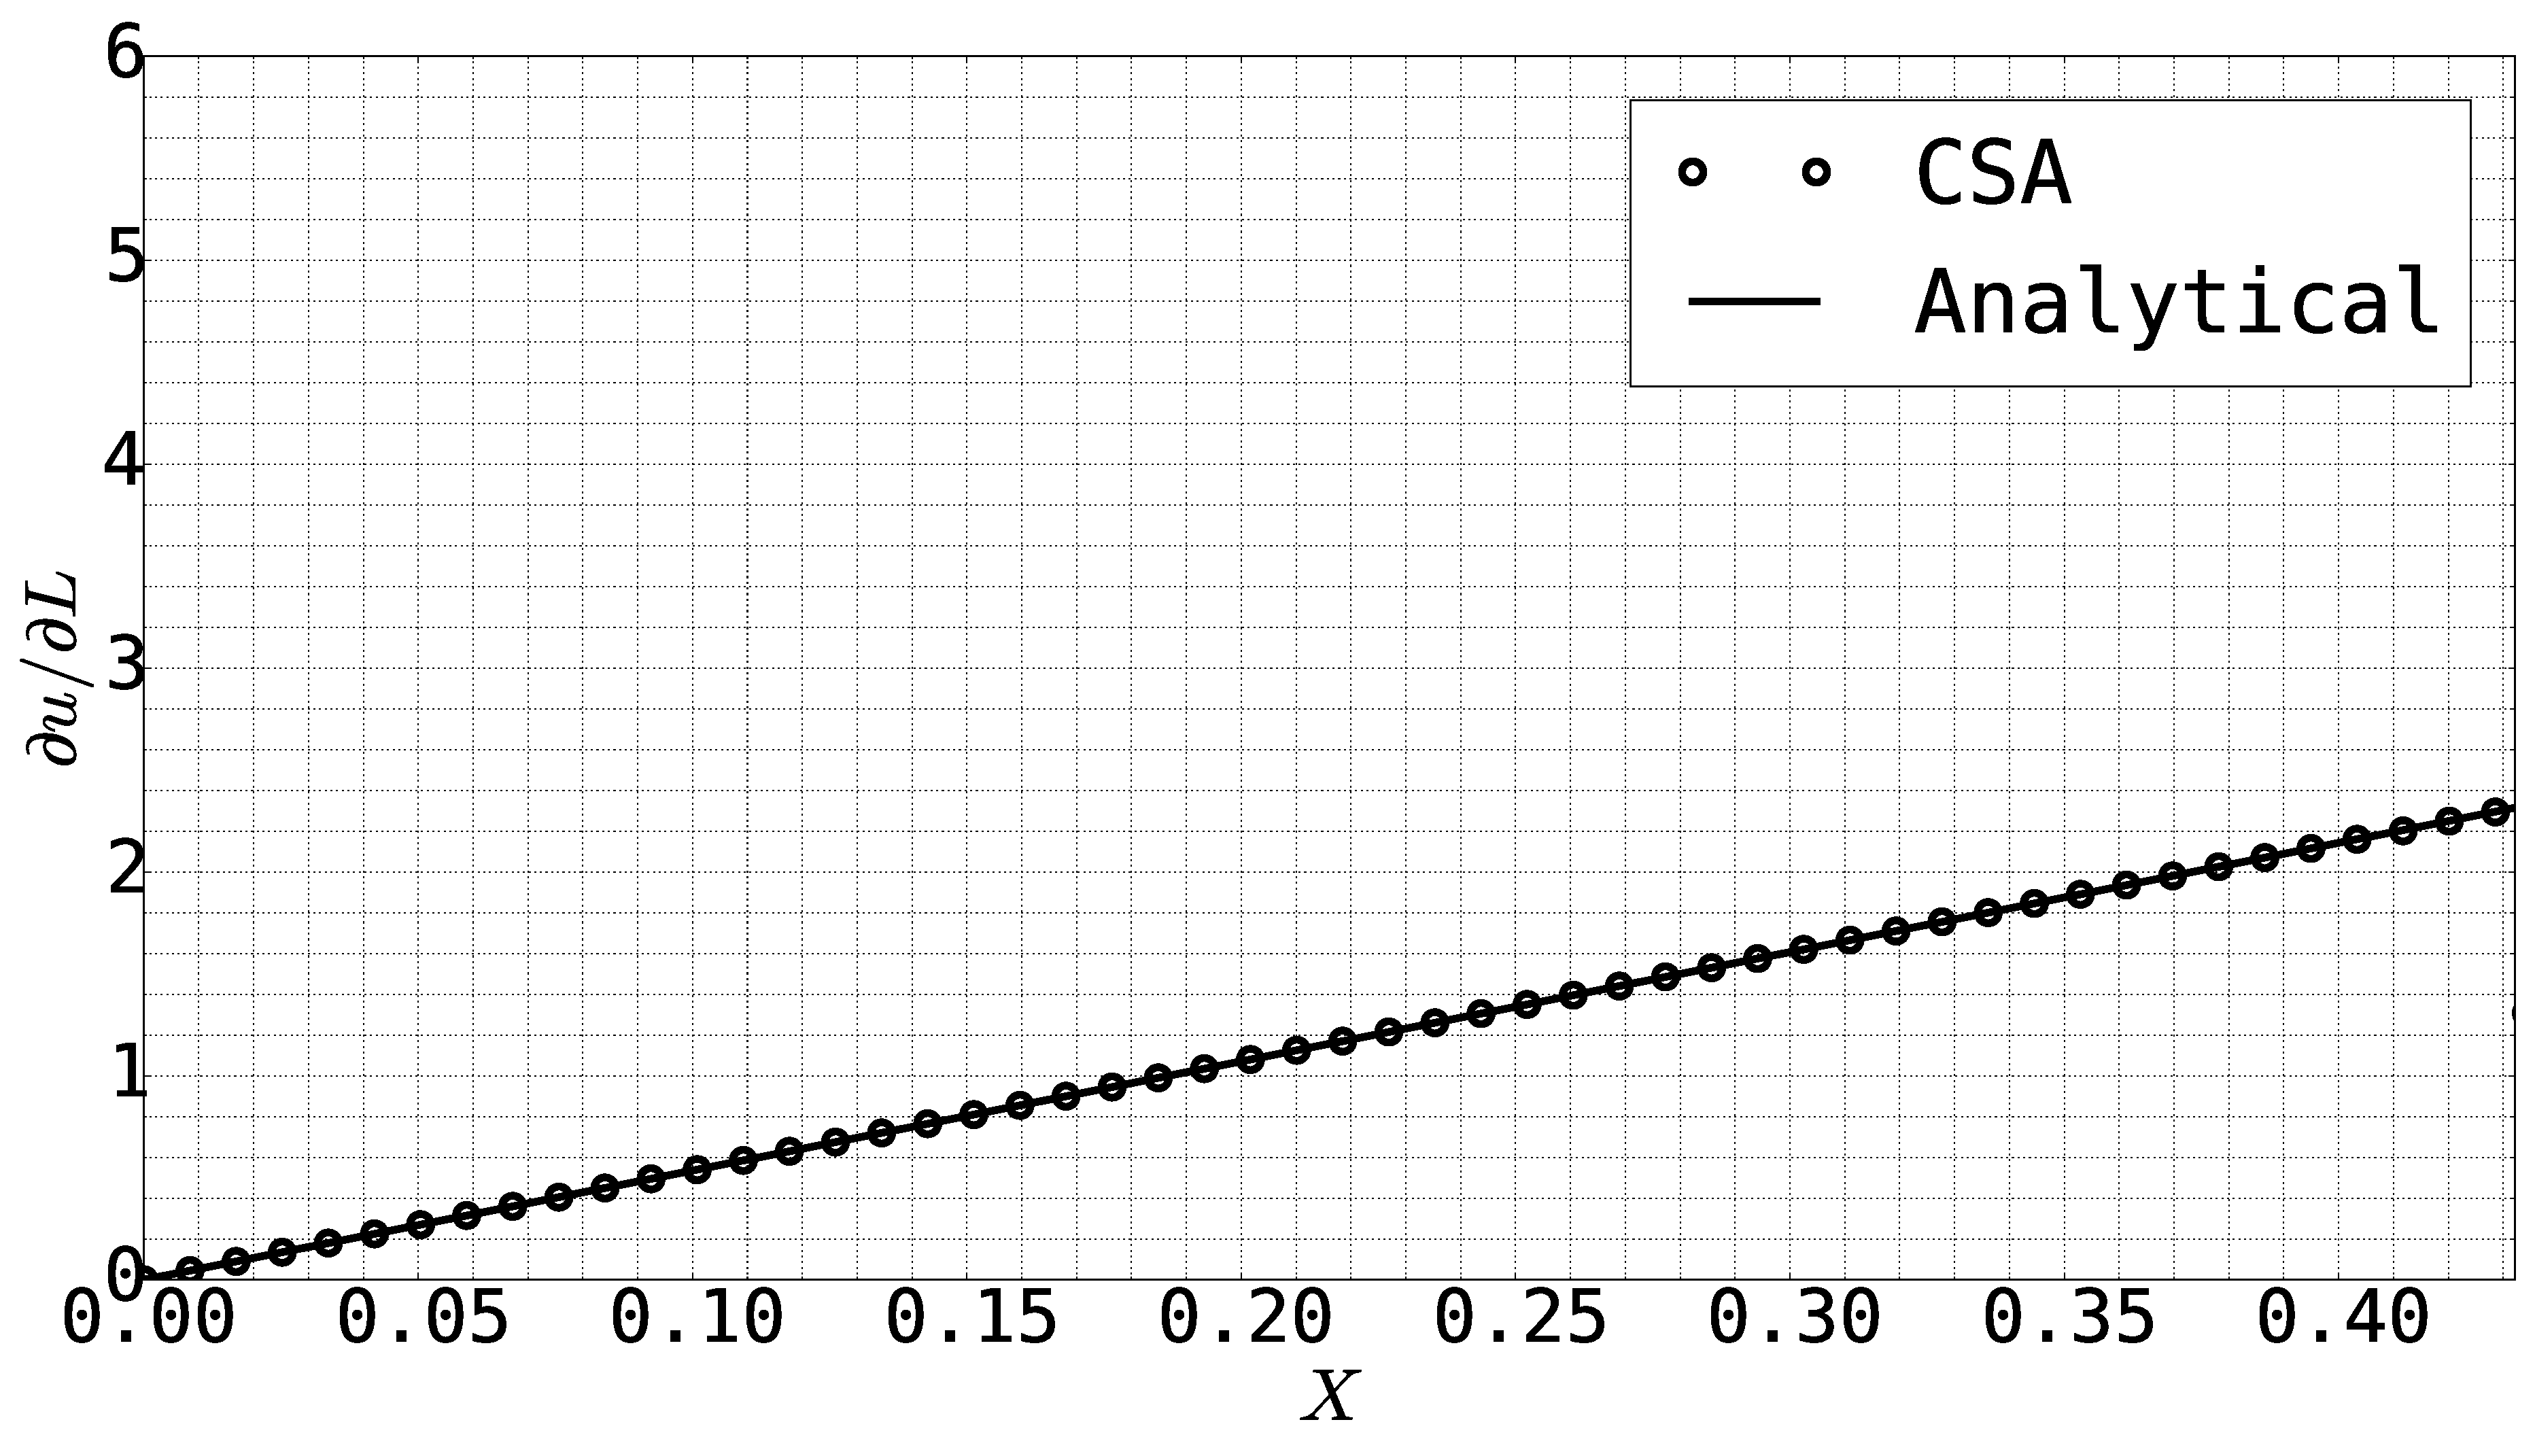
\includegraphics[width=7.0cm]{Chapter_4/figure/penalizationMethod_sensitivityProfile_reconstructed_xw04321.eps}
    }
    \quad
    \subfigure[$x_{wall} = 0.7583, n = 120$]
    {
    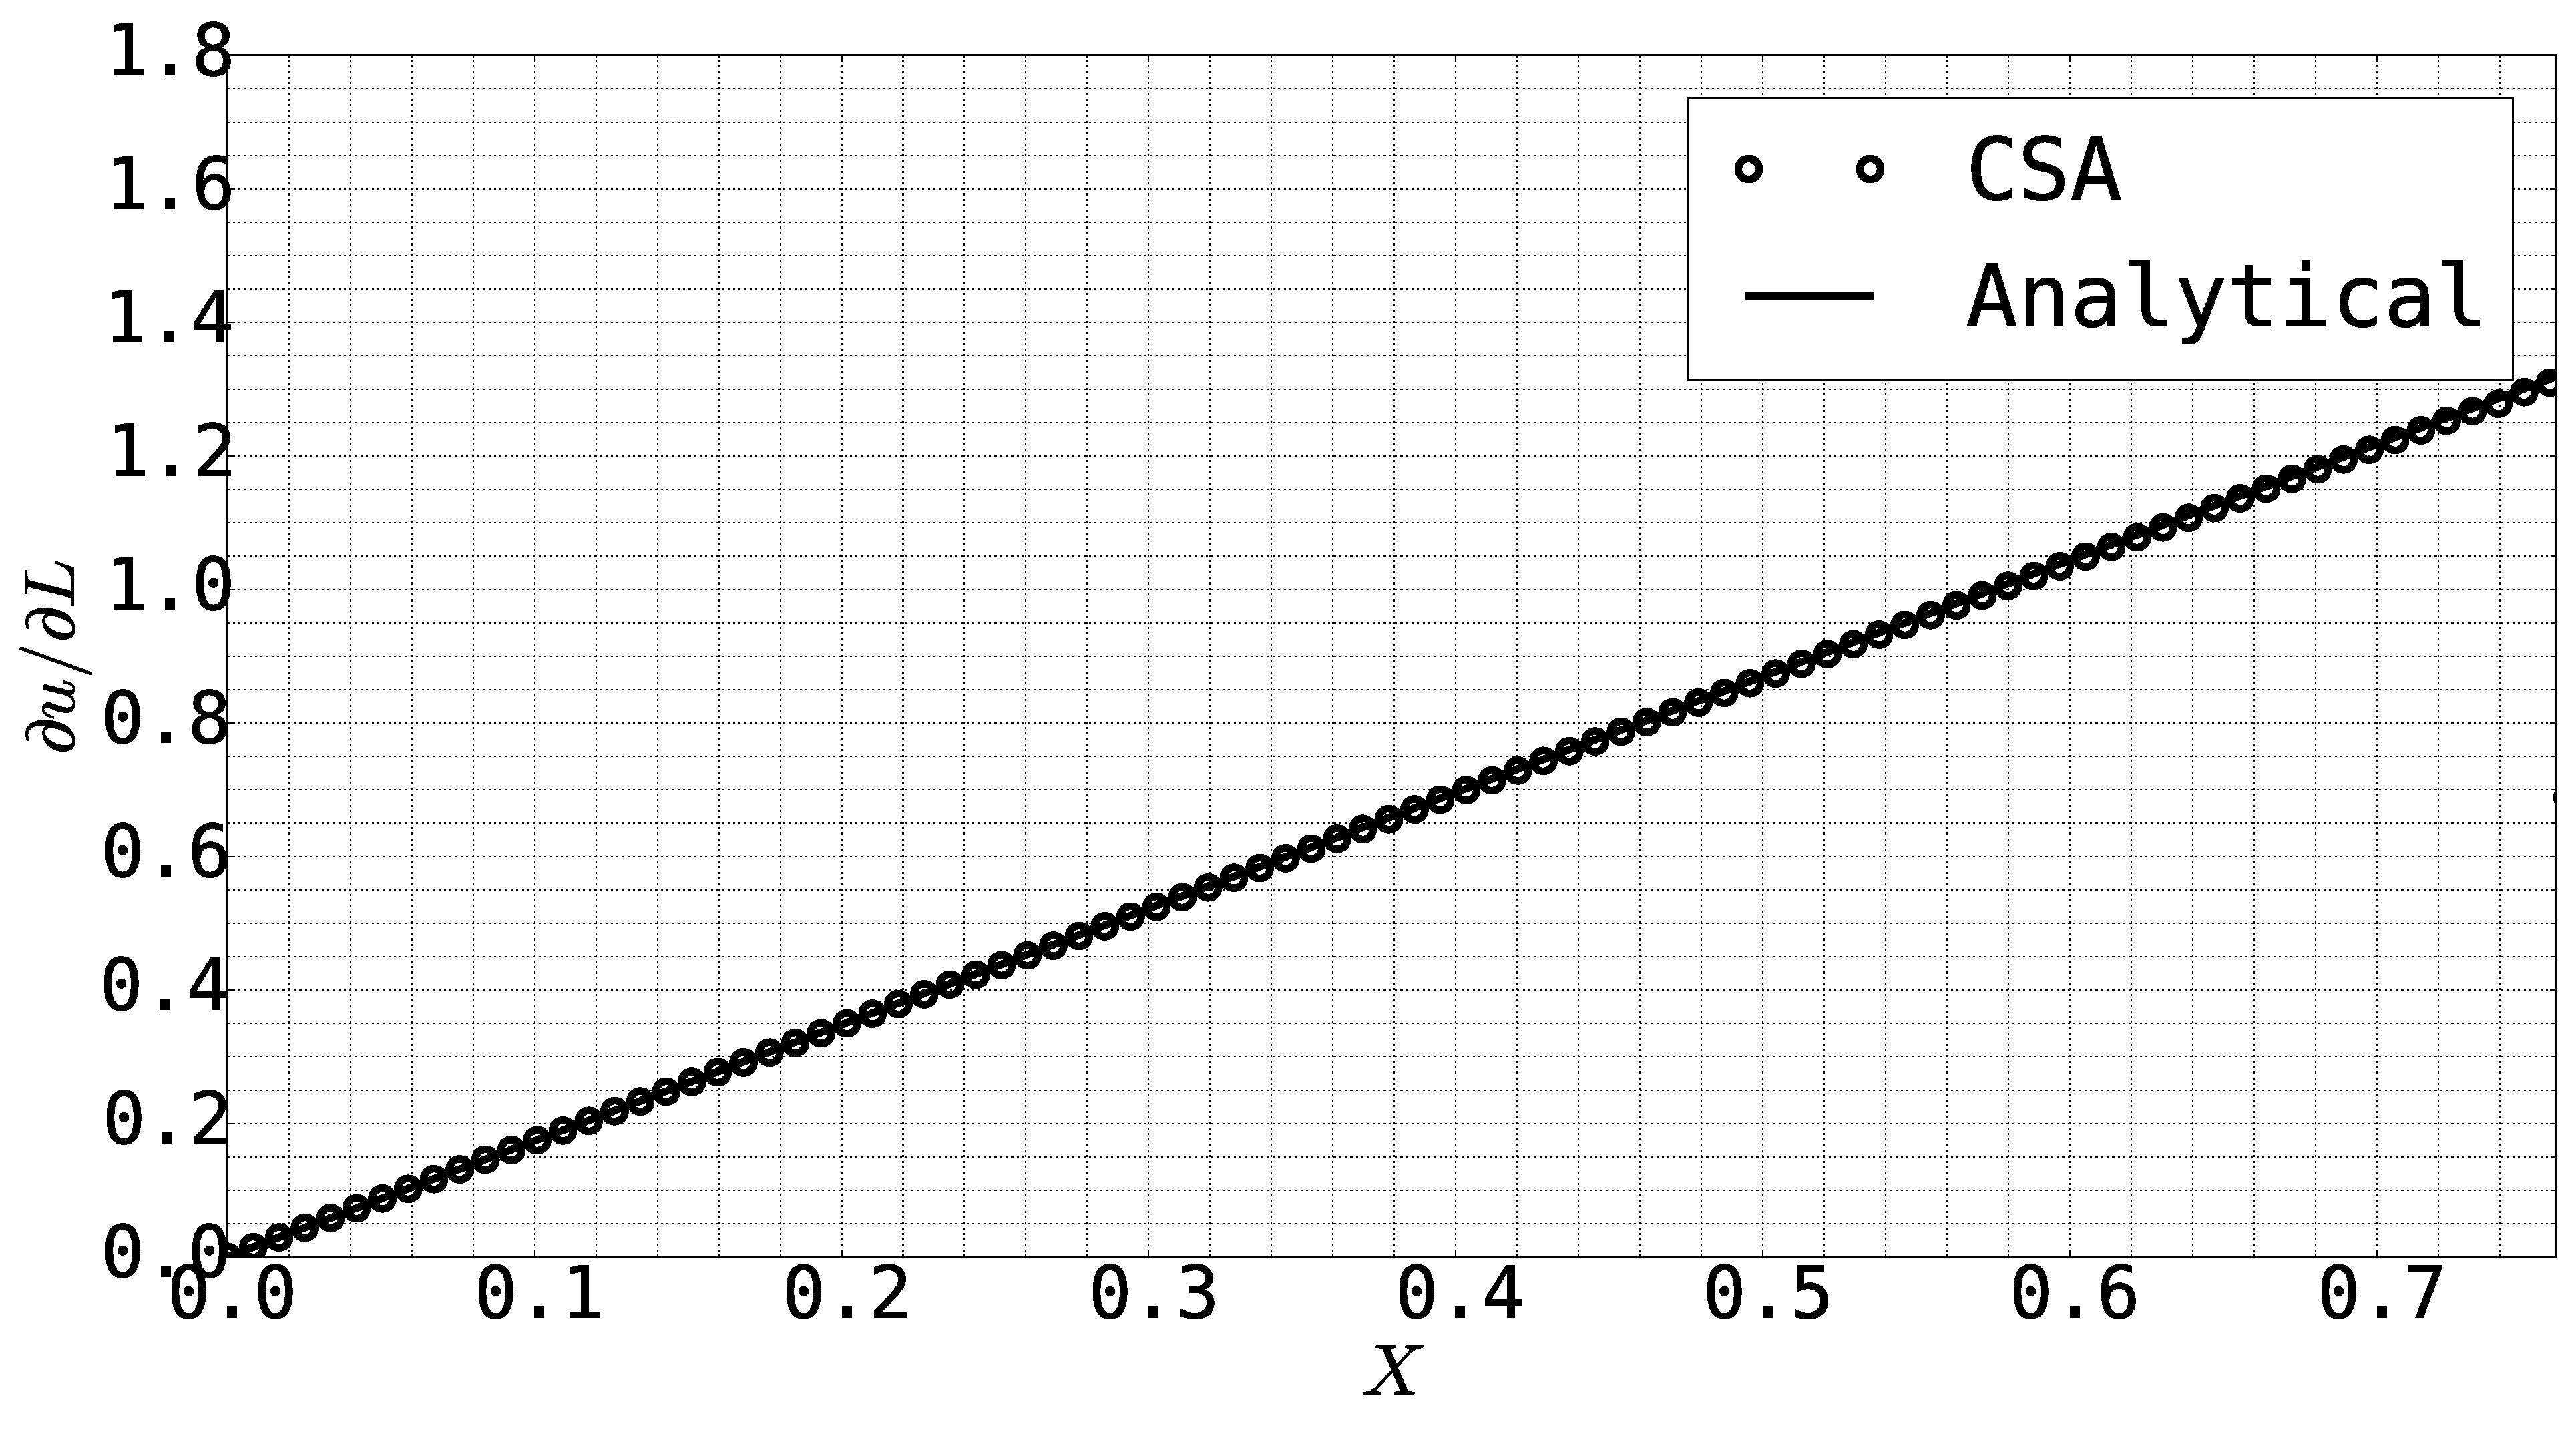
\includegraphics[width=7.0cm]{Chapter_4/figure/penalizationMethod_sensitivityProfile_reconstructed_xw07583.eps}
    }
    \\
    \subfigure[$x_{wall} = 0.2451, n = 30$]
    {
    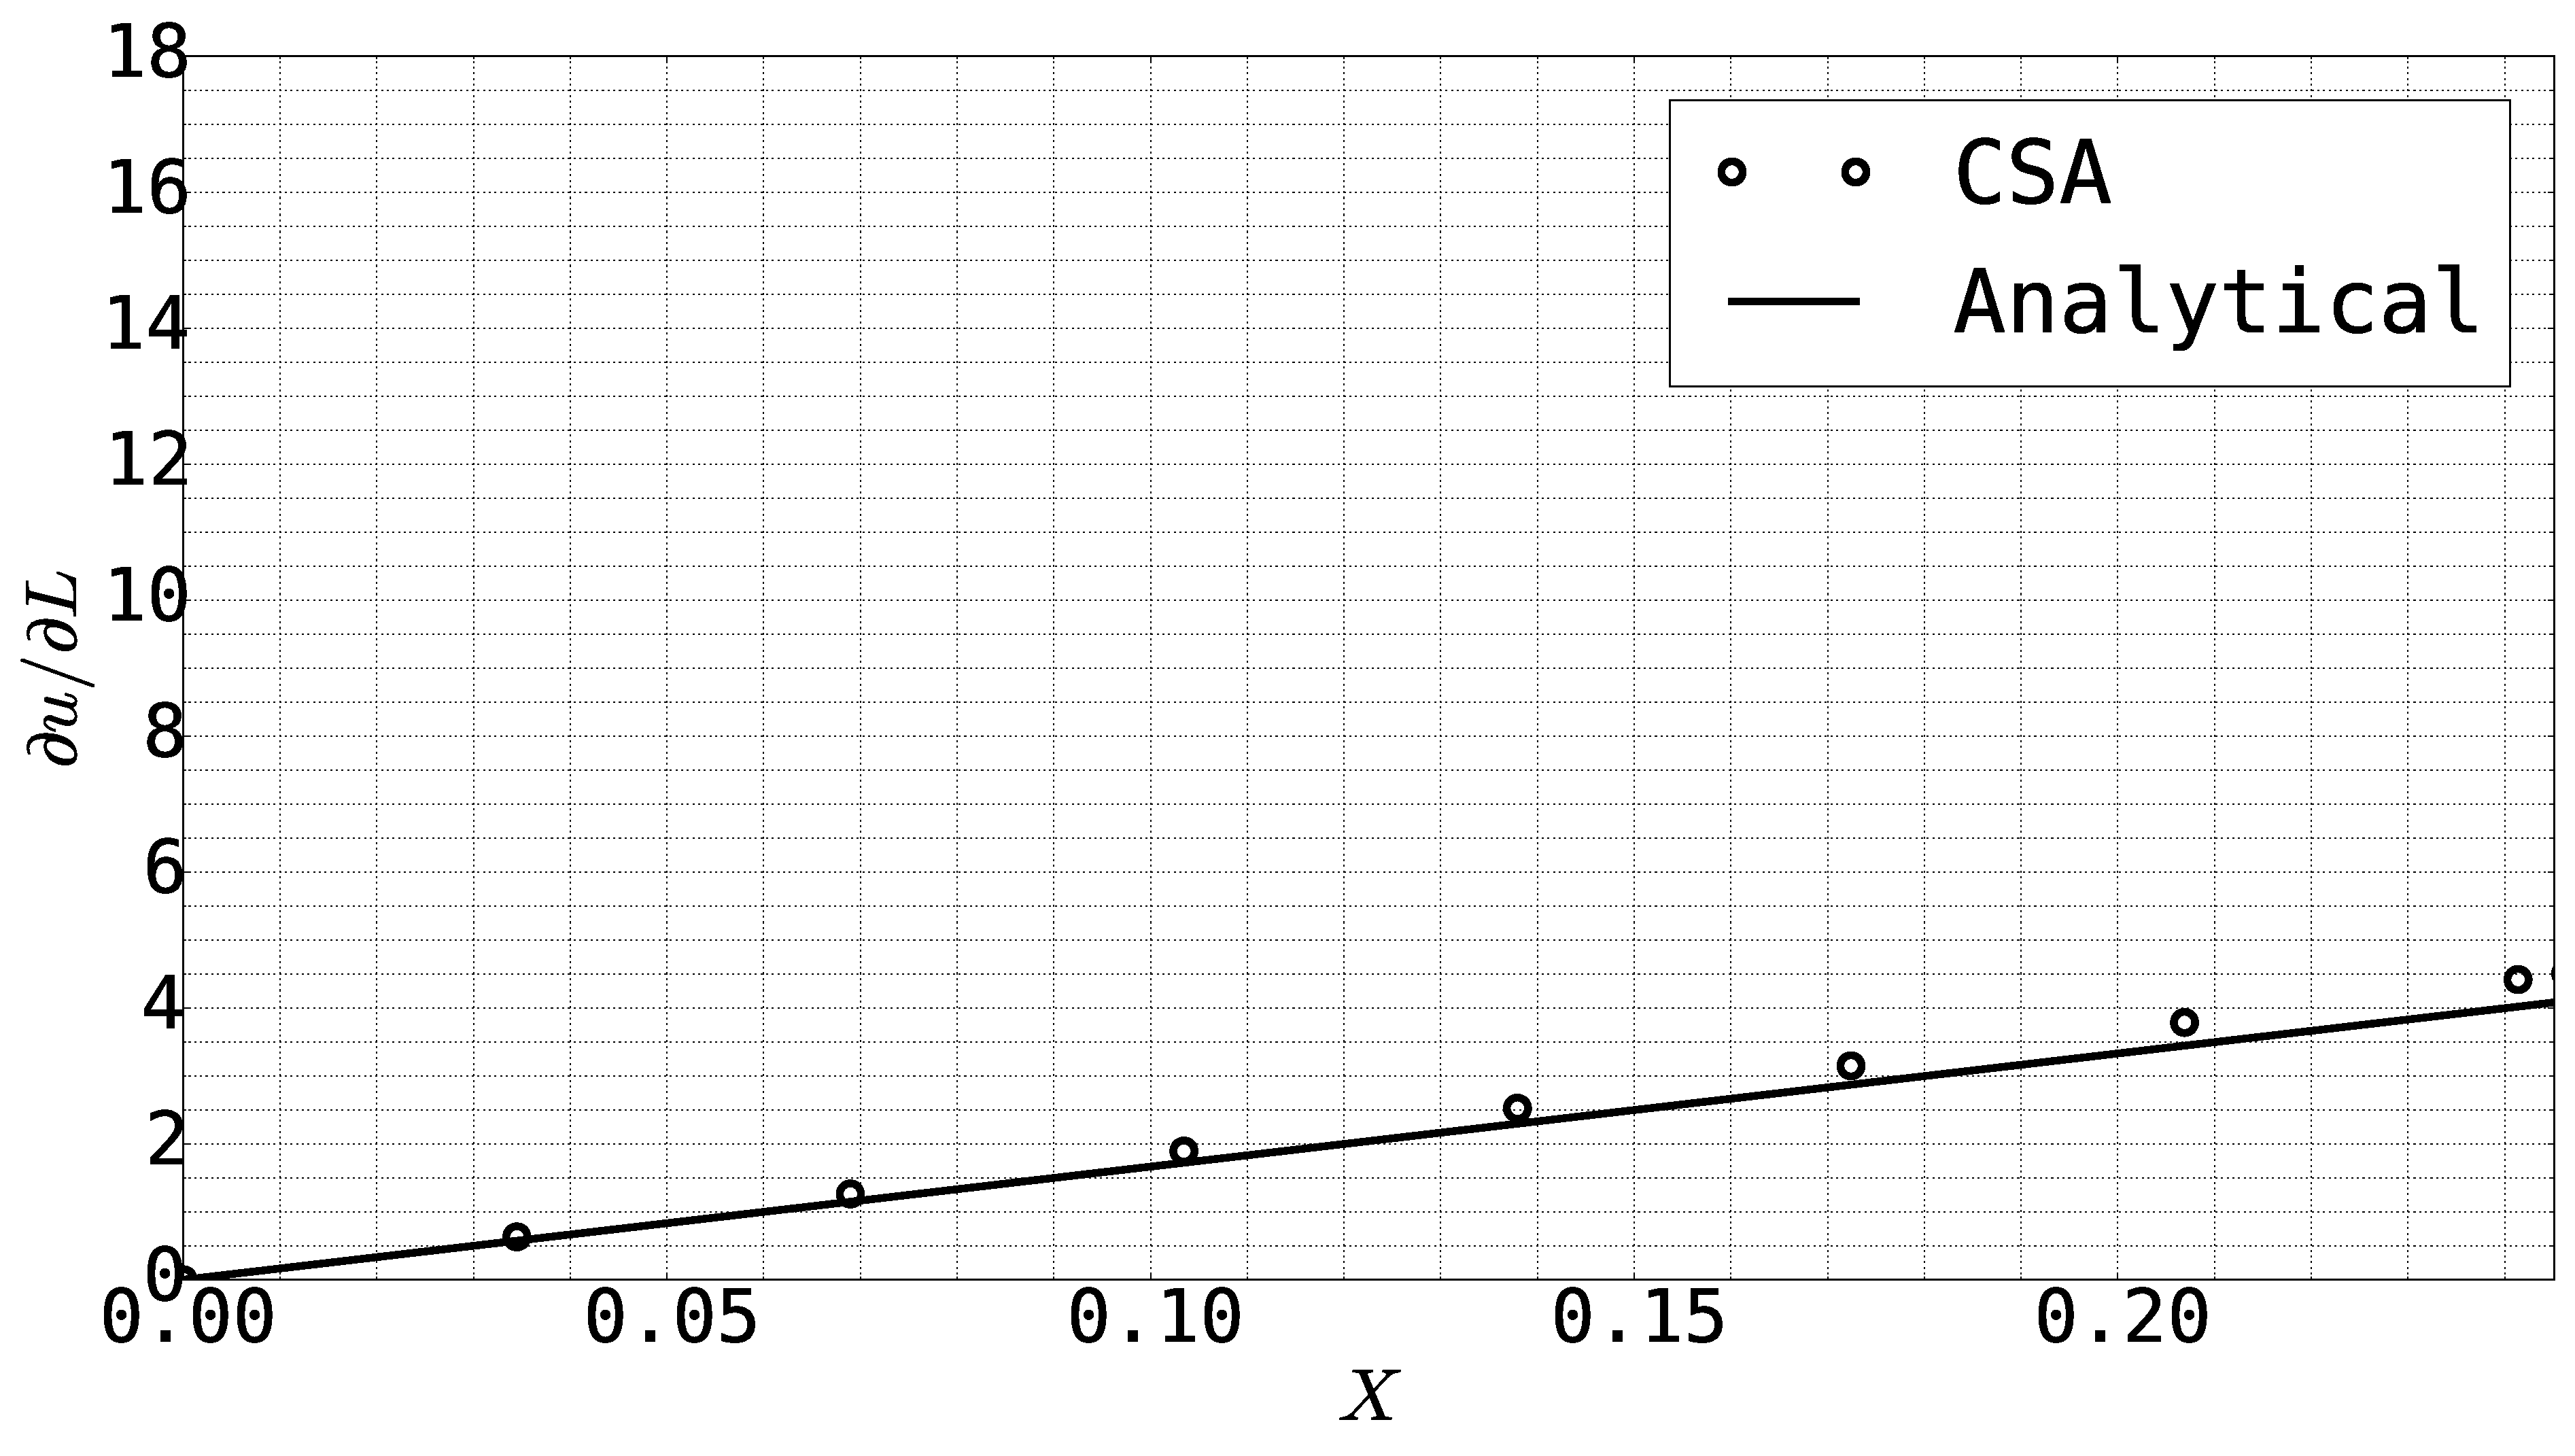
\includegraphics[width=7.0cm]{Chapter_4/figure/penalizationMethod_sensitivityProfile_reconstructed_xw02451.eps}
    }
    \quad
    \subfigure[$x_{wall} = 0.5742, n = 60$]
    {
    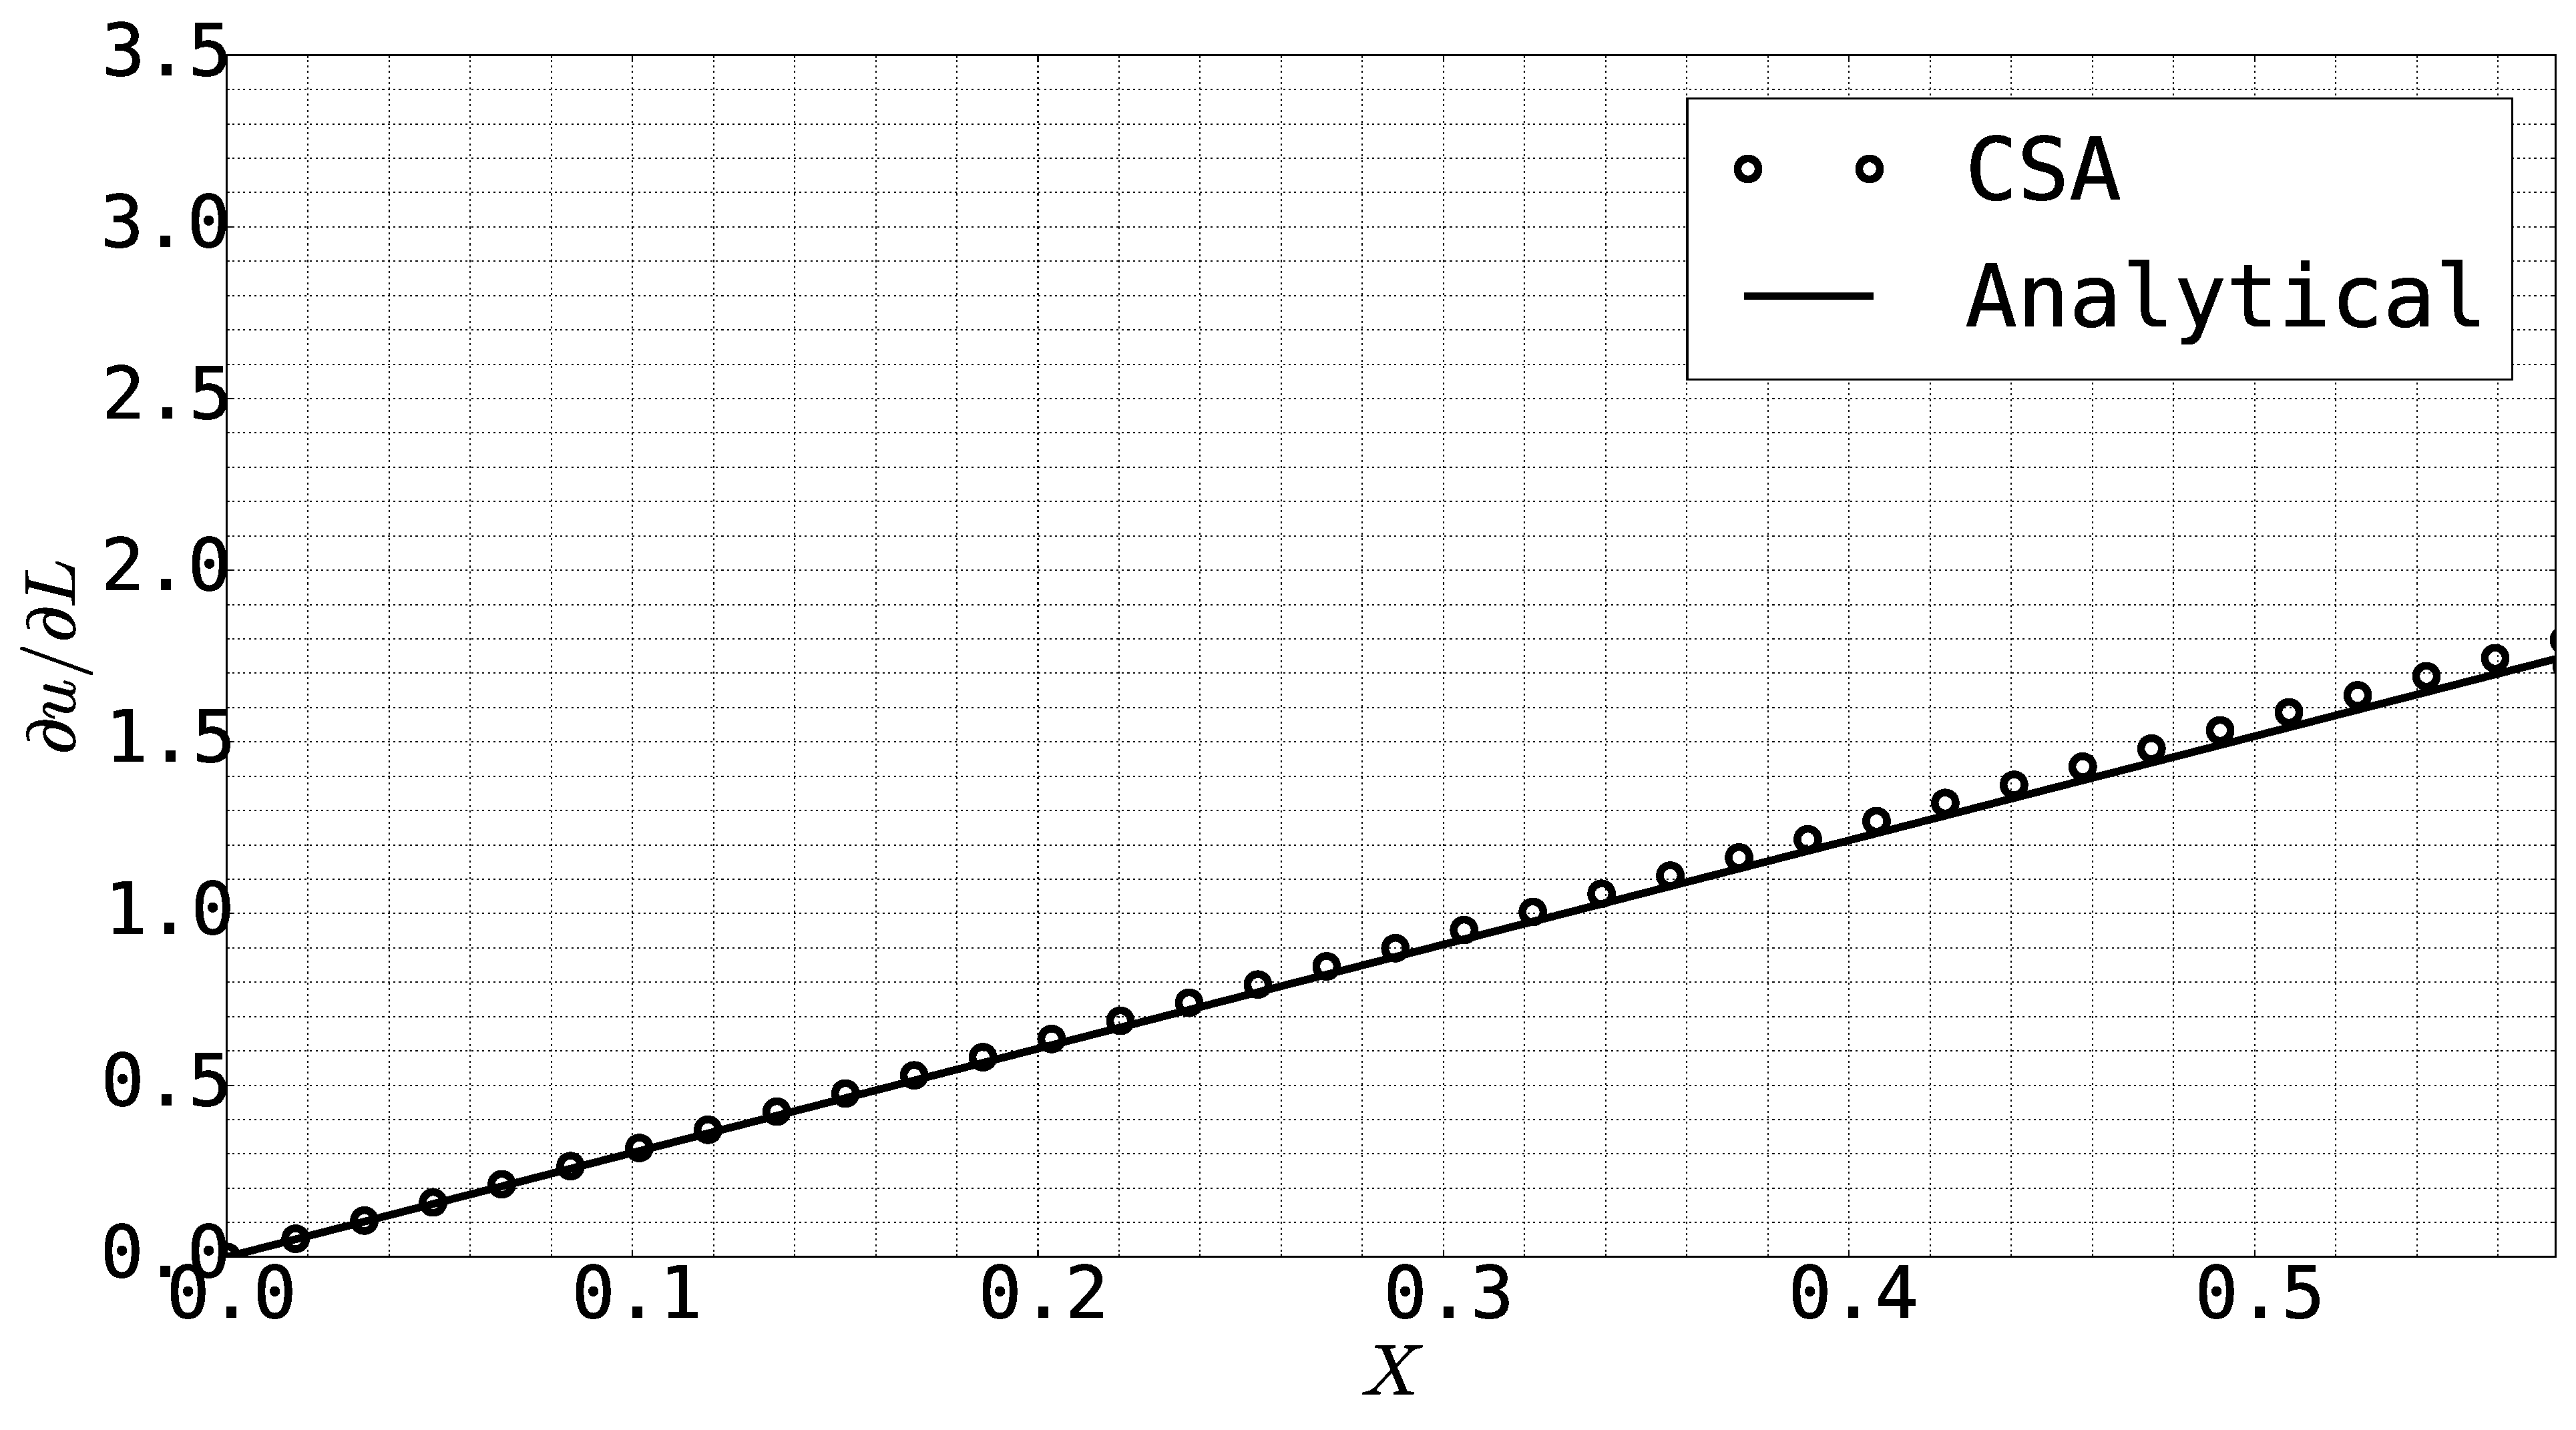
\includegraphics[width=7.0cm]{Chapter_4/figure/penalizationMethod_sensitivityProfile_reconstructed_xw05742.eps}
    }
    \caption{Reconstructed sensitivity by post-processing the results.}
    \label{fig:C4_sensitivityResultsReconstructed1Dproblem}
\end{figure}

This problem is also solved using the virtual boundary method and the results are compared with the penalization method in terms of accuracy of simulation cost. The simulation cost is defined as number of time steps it takes to reach a converged value. The virtual boundary method is based on solving the Navier-Stokes equation \eqref{eq:C4_NS} and modeling the boundaries through the force term defined in Equation \eqref{eq:C3_feedbackForcingFunction}. As mentioned in the Section \ref{sec:C4_RHandRDfunction}, the RD function need to be used in the virtual boundary method to have a differentiable governing equation for CSA. Therefore, the effect of RD function on the accuracy of the solution is first investigated.

The RD function for this simulation is selected as the one in Equation \eqref{eq:C4_deltaFunction}. The $\eta$ parameter is based on Equation \eqref{eq:C4_etaGuideForRDfunction} where $p = 0.99$ and $R = 2dx$. This ensures the stability of the solution. For this analysis $\alpha$ and $\beta$ constants in Equation \eqref{eq:C3_feedbackForcingFunction} are each selected as $-100$. The convergence result is shown in Figure \ref{fig:C4_virtualBoundary_RDvsD}. As shown here, the simulation with RD function has better convergence properties.

\begin{figure}[H]
	\centering
	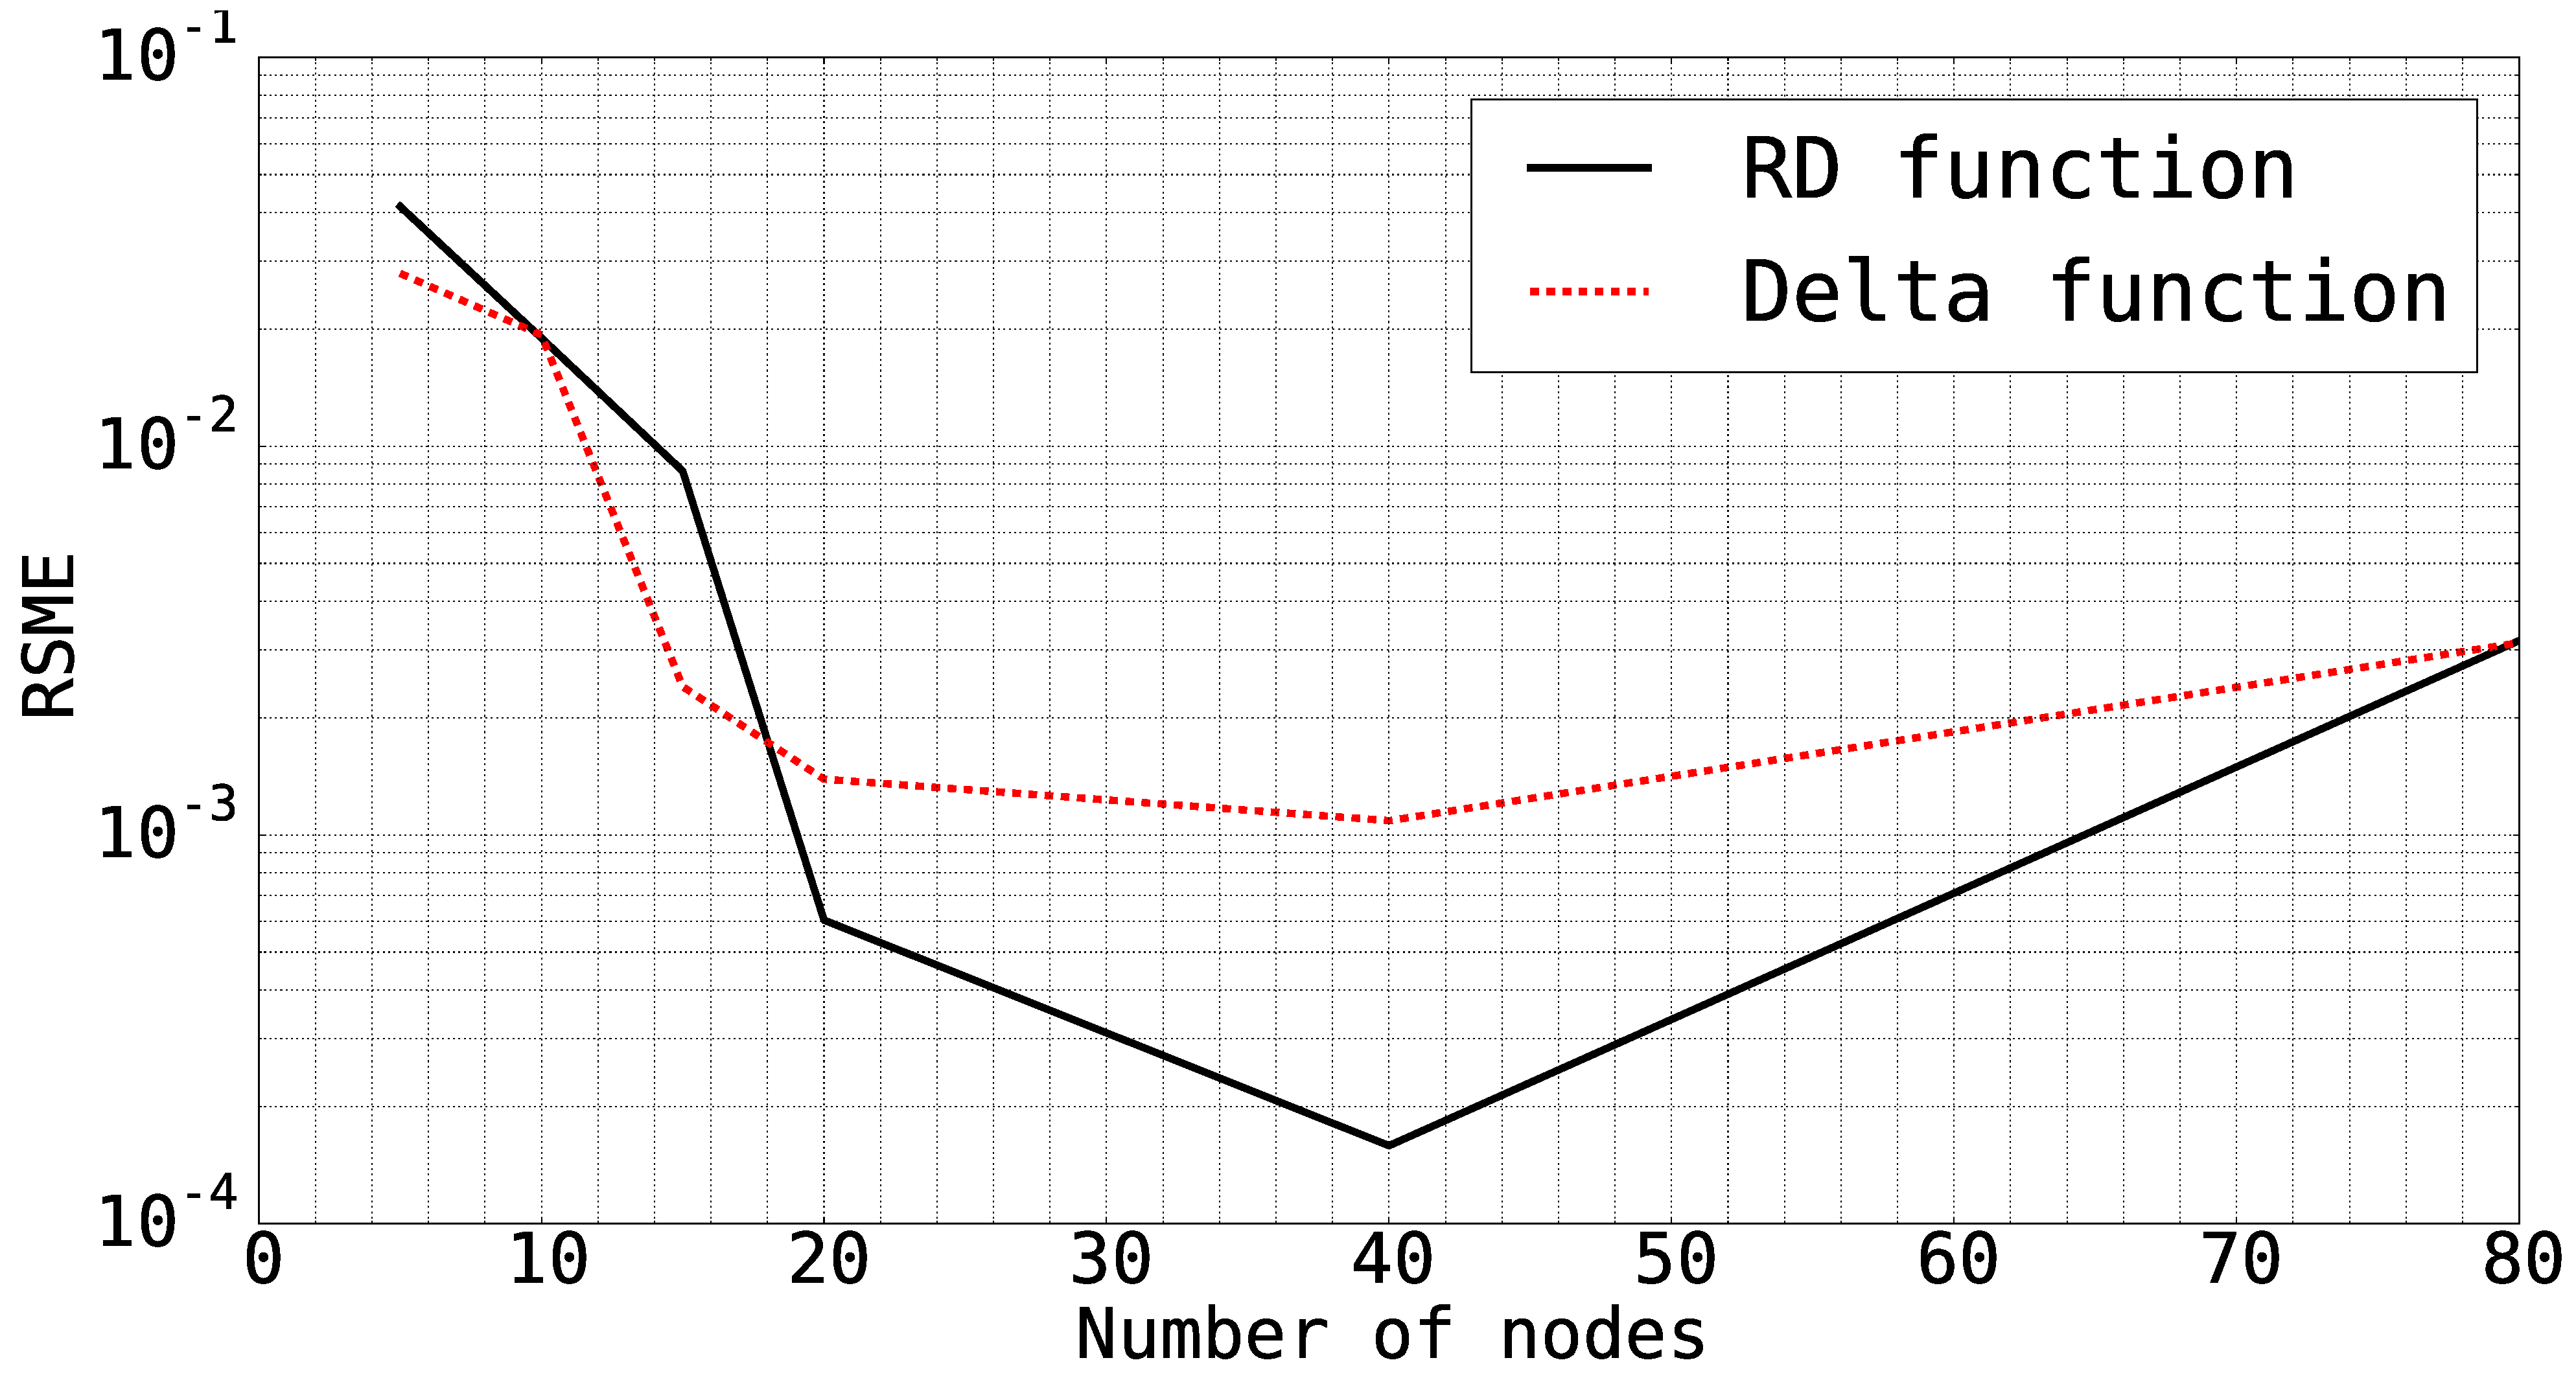
\includegraphics[width=12.00cm]{Chapter_4/figure/effect_of_RD_on_simulation_vs_numberOfNodes_1D_problem.eps}
	\caption{Effect of Regularized Delta (RD) and delta function on the solution accuracy.}
	\label{fig:C4_virtualBoundary_RDvsD}
\end{figure}

The effect of wall velocity of the accuracy of the simulation was also investigated. The wall velocity was selected as $1 m/s$, $10 m/s$, $100 m/s$, and $1000 m/s$. However, this did not affect the accuracy of the simulation.

The sensitivity equations are derived by differentiating the Navier-Stokes equations as shown in Equation \eqref{eq:C4_NSwithvirtualBoundaryIBsensitivity}. However, for this problem Equation \eqref{eq:C4_NSwithvirtualBoundaryIBsensitivity} is simplified as shown in Equation \eqref{eq:C4_SAforVirtualBoundaryMethod1D}.

\begin{align}\label{eq:C4_SAforVirtualBoundaryMethod1D}
    \frac{\partial u'}{\partial t}
    &= 
    \nu \nabla^2 u' + \nonumber \\
    &\left\{
    \alpha
    \int_0^t
    \left[
        \int u'(x, \tau) \mathcal{D}(x - X) d\mathbf{x} + 
        \int u(x, \tau) \frac{\partial \mathcal{D}}{\partial X} \frac{\partial X}{\partial b} d\mathbf{x}
    \right] d\tau \right.
    + \nonumber \\
    &
    \left.
    \beta
    \left[
    \int u'(x, t) \mathcal{D}(x - X) d\mathbf{x} +
    \int u(x, t) \frac{\partial \mathcal{D}}{\partial X} \frac{\partial X}{\partial b} d\mathbf{x}
    \right]
    \right\} \bar{\mathcal{D}}(x - X) + \nonumber \\
    &\left\{
    \alpha
    \int_0^t
    \left[
        \int u(x, \tau) \mathcal{D}(x - X) d\mathbf{x}
    \right] d\tau
    +
    \beta
    \int u(x, t) \mathcal{D}(x - X) d\mathbf{x}
    \right\}
    \frac{\partial \bar{\mathcal{D}}}{\partial X} \frac{\partial X}{\partial b}
\end{align}

where $X$ is the location of the wall. Equation \eqref{eq:C4_SAforVirtualBoundaryMethod1D} required the calculation of the RD function of Equation \eqref{eq:C4_deltaFunction}. This function is known as the doublet function \cite{kamaraju2009linear} and is written as shown in Equation \eqref{eq:C4_doubletFunction}. The $\eta$ value for this function is the same one chosen for the RD function. The double function of Equation \eqref{eq:C4_doubletFunction} is plotted in Figure \ref{fig:C4_doubletFunction} for different values of $\eta$.

\begin{equation}\label{eq:C4_doubletFunction}
	T(x, \eta) = 
	\frac{\left[ \tanh^{2}{\left(\dfrac{x}{t} \right)} - 1 \right] \tanh{\left( \dfrac{x}{t} \right)}}{t^2} 
\end{equation}

\begin{figure}[H]
	\centering
	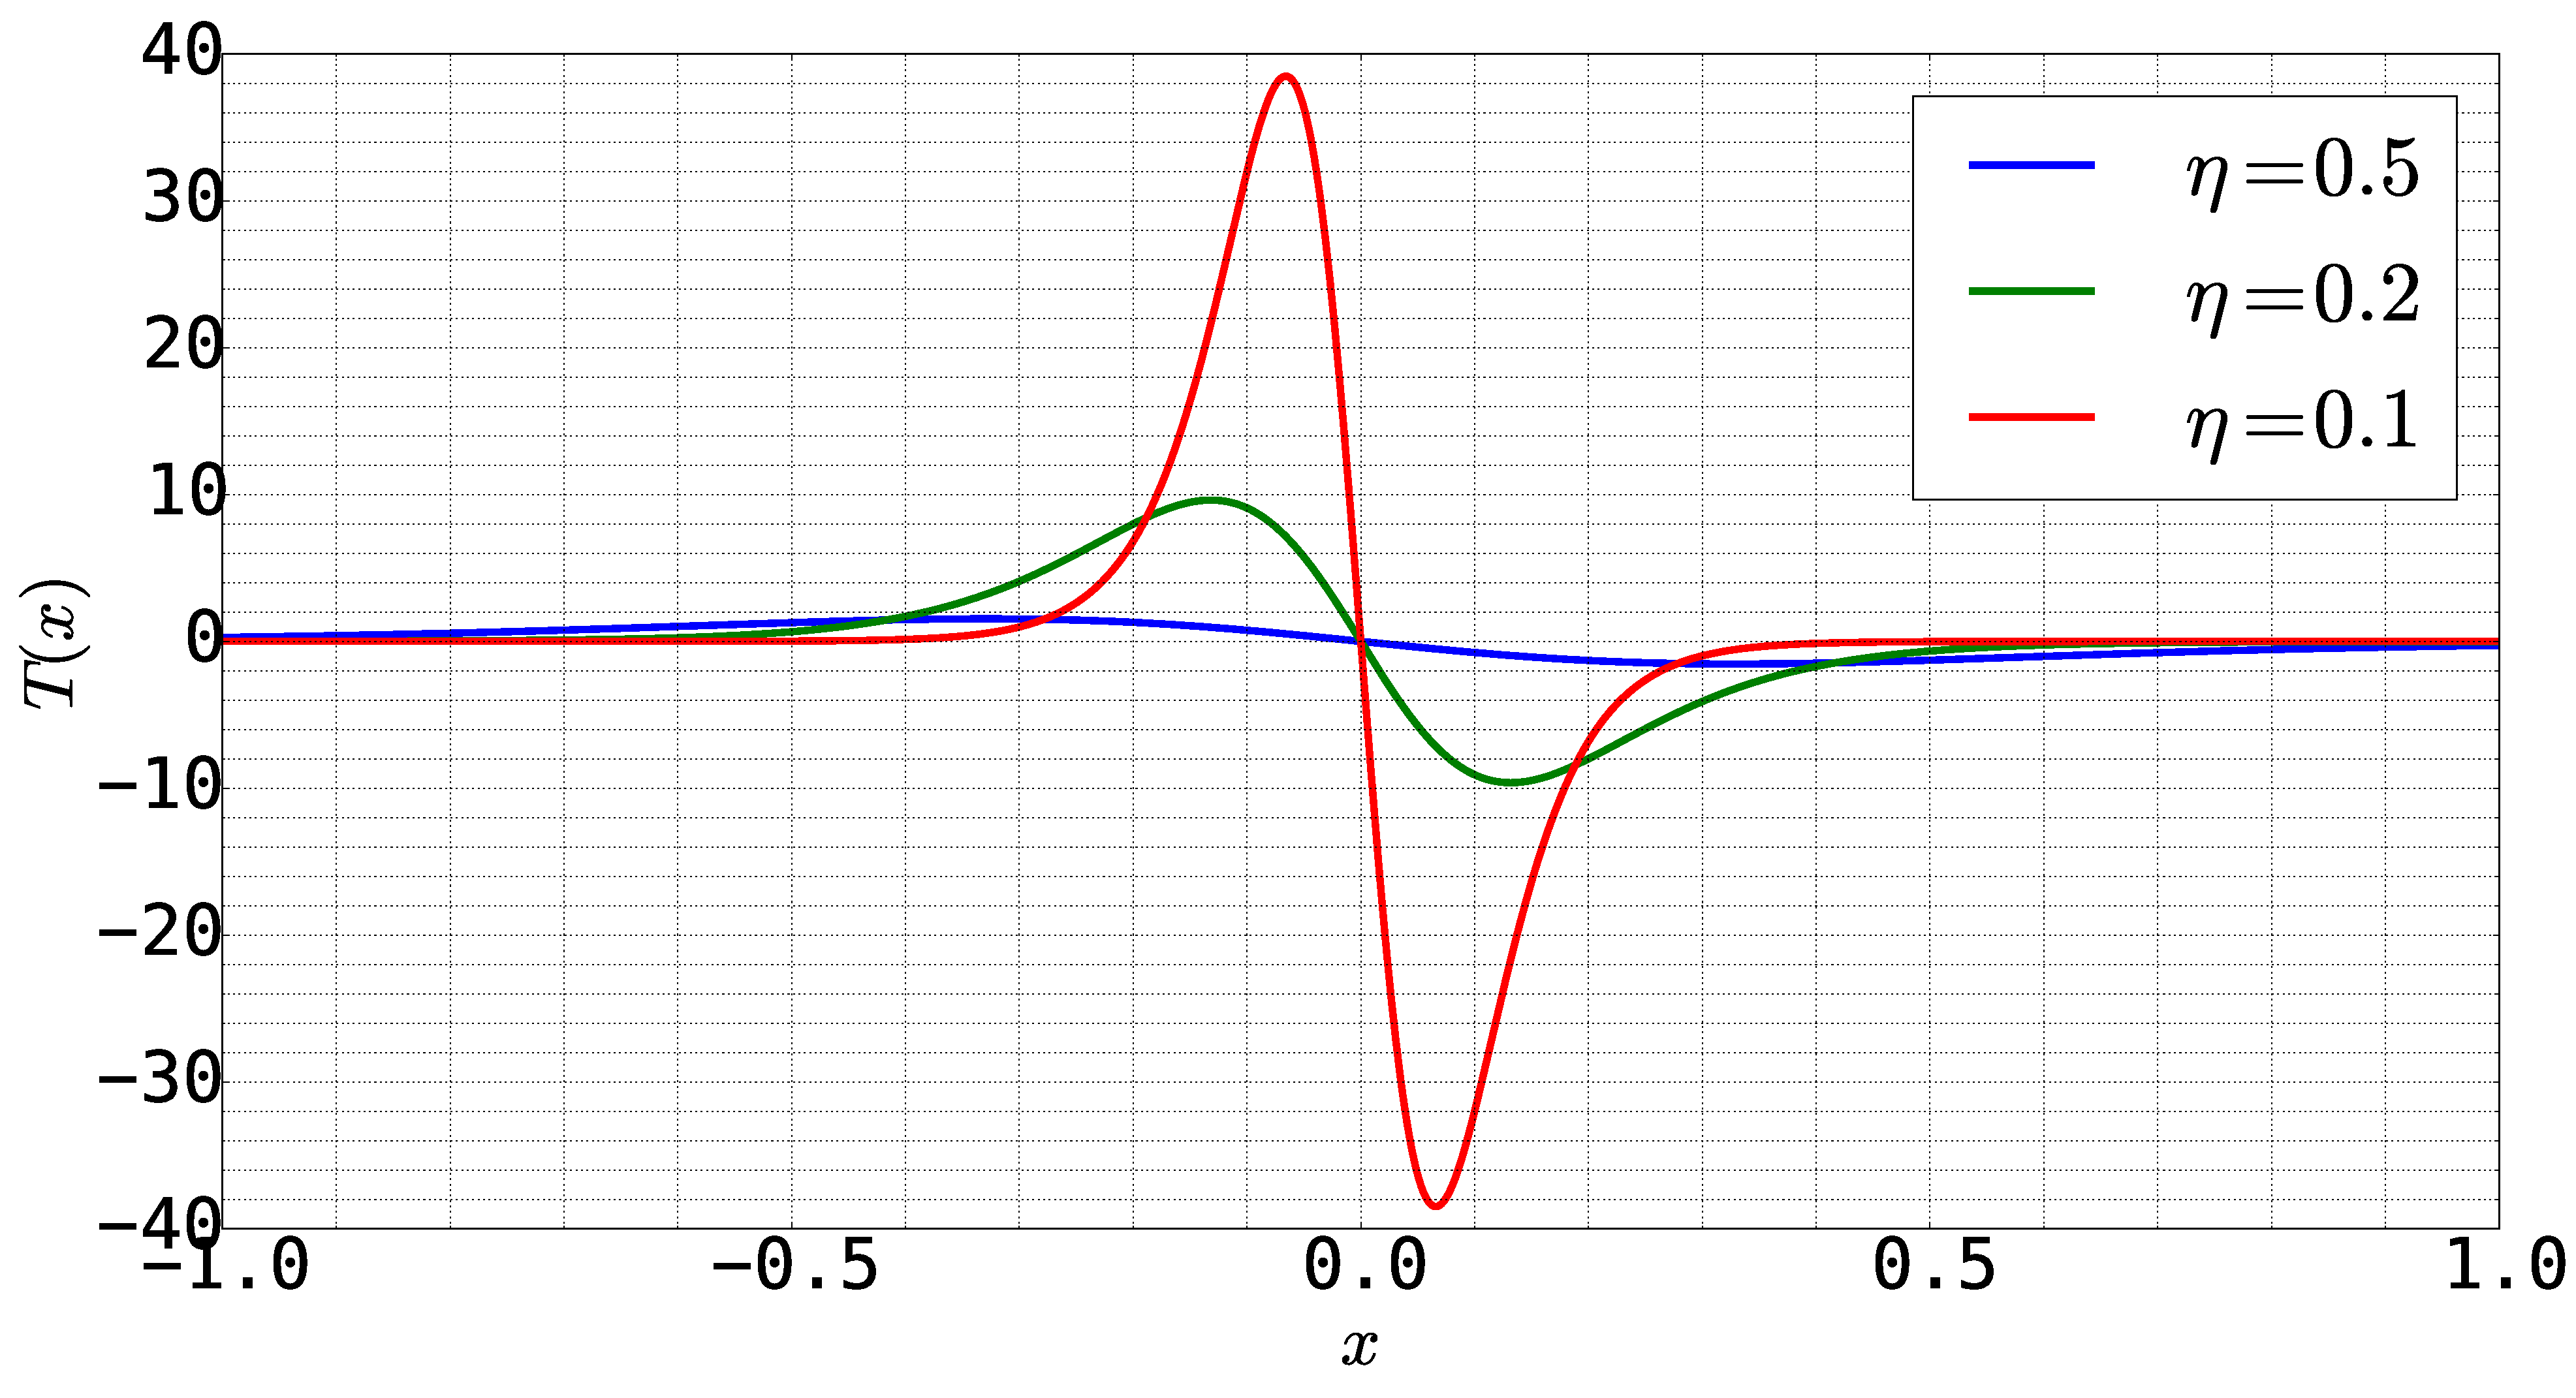
\includegraphics[width=12.00cm]{Chapter_4/figure/doubletFunction.eps}
	\caption{Doublet function of Equation \eqref{eq:C4_doubletFunction}.}
	\label{fig:C4_doubletFunction}
\end{figure}

The boundary conditions for Equation \eqref{eq:C4_SAforVirtualBoundaryMethod1D} is defined by differentiating the boundary conditions in Equation \eqref{eq:C4_1DbenchmarkBoundaryCondition}. Since neither of these boundary conditions depend on the design variable, the boundary conditions for Equation \eqref{eq:C4_SAforVirtualBoundaryMethod1D} is equal to zero. This is defined in Equation \eqref{eq:C4_SAboundaryConditionforVirtualBoundaryMethod1D}.

\begin{equation}\label{eq:C4_SAboundaryConditionforVirtualBoundaryMethod1D}
\begin{cases}
	u' = 0 \qquad \text{at } x = 0 \\
	u' = 0 \quad \text{at } x = 1
\end{cases}
\end{equation}

The analytical results of the sensitivity of velocity profile to the length is defined in Equation \eqref{eq:C4_1DbenchmarkAnalyticalSAlength} and used for verifying the sensitivity results.

The convergence results for the sensitivity analysis are shown in Figure \ref{fig:C3_virtualBoundarySAconvergence}.
% ======================================================================
\section{Shape Sensitivity of Flow over a Cylinder}
% ==================================================
For the second demonstration problem, the flow over a cylinder is modeled using the virtual boundary method using Equation \eqref{eq:C4_NSwithvirtualBoundaryIB}. The sensitivity analysis is conducted by differentiating the NS equations as shown in Equation \eqref{eq:C4_NSwithvirtualBoundaryIBsensitivity}. For this problem the domain is defined as a rectangle with the cylinder located on the horizontal symmetry line as shown in Figure \ref{fig:C4_cylinderPhysicalDomain}.

\begin{figure}[H]
    \centering
    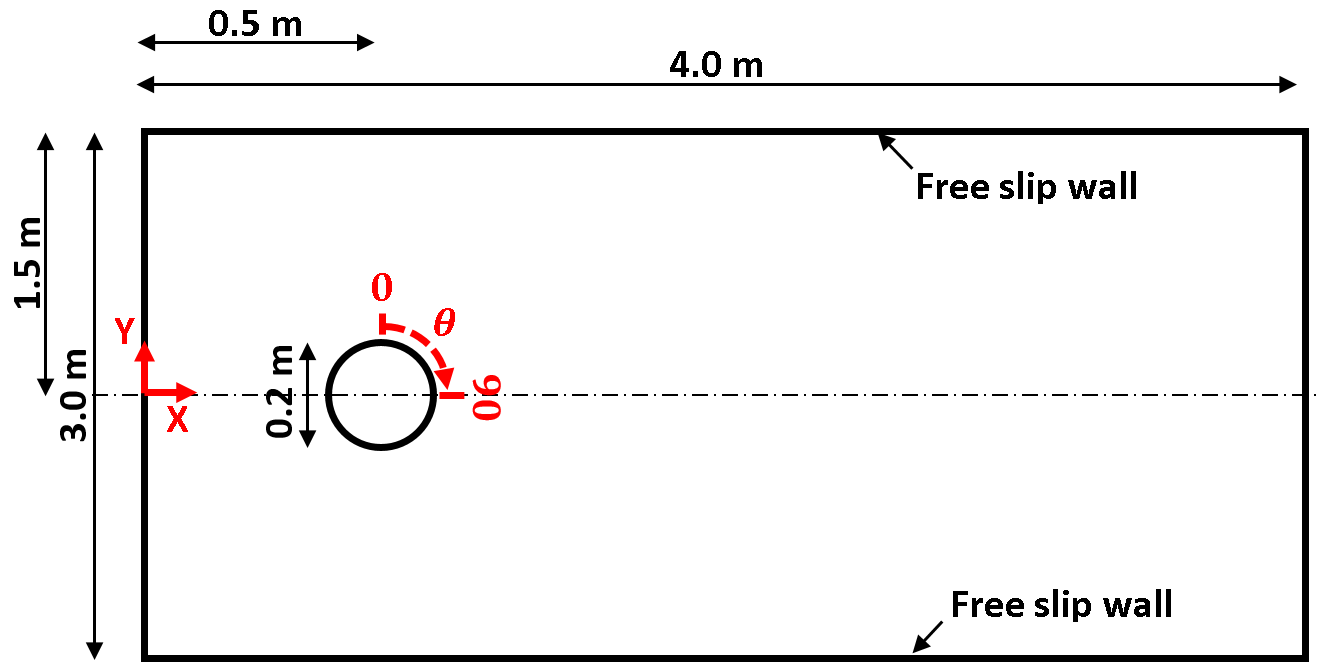
\includegraphics[width=12.00cm]{Chapter_4/figure/flow_over_cylinder/flow_over_cylinder.png}
    \caption{Physical domain with dimensions for flow over cylinder.}
    \label{fig:C4_cylinderPhysicalDomain}
\end{figure}

The boundary conditions are defined as the flow velocity at the inlet (left boundary) and the outflow (zero gradient) boundary condition at the outlet (right boundary). The top and bottom boundaries are modeled as free slip walls. The surface of the cylinder is modeled by the virtual boundary method. The mesh convergence for this problem for Reynolds number of 100 is shown in Figure \ref{fig:C4_meshConvergenceForCylidnerRE100GE}.

\begin{figure}[H]
    \centering
    \subfigure[U-velocity on y = 0.]
    {
    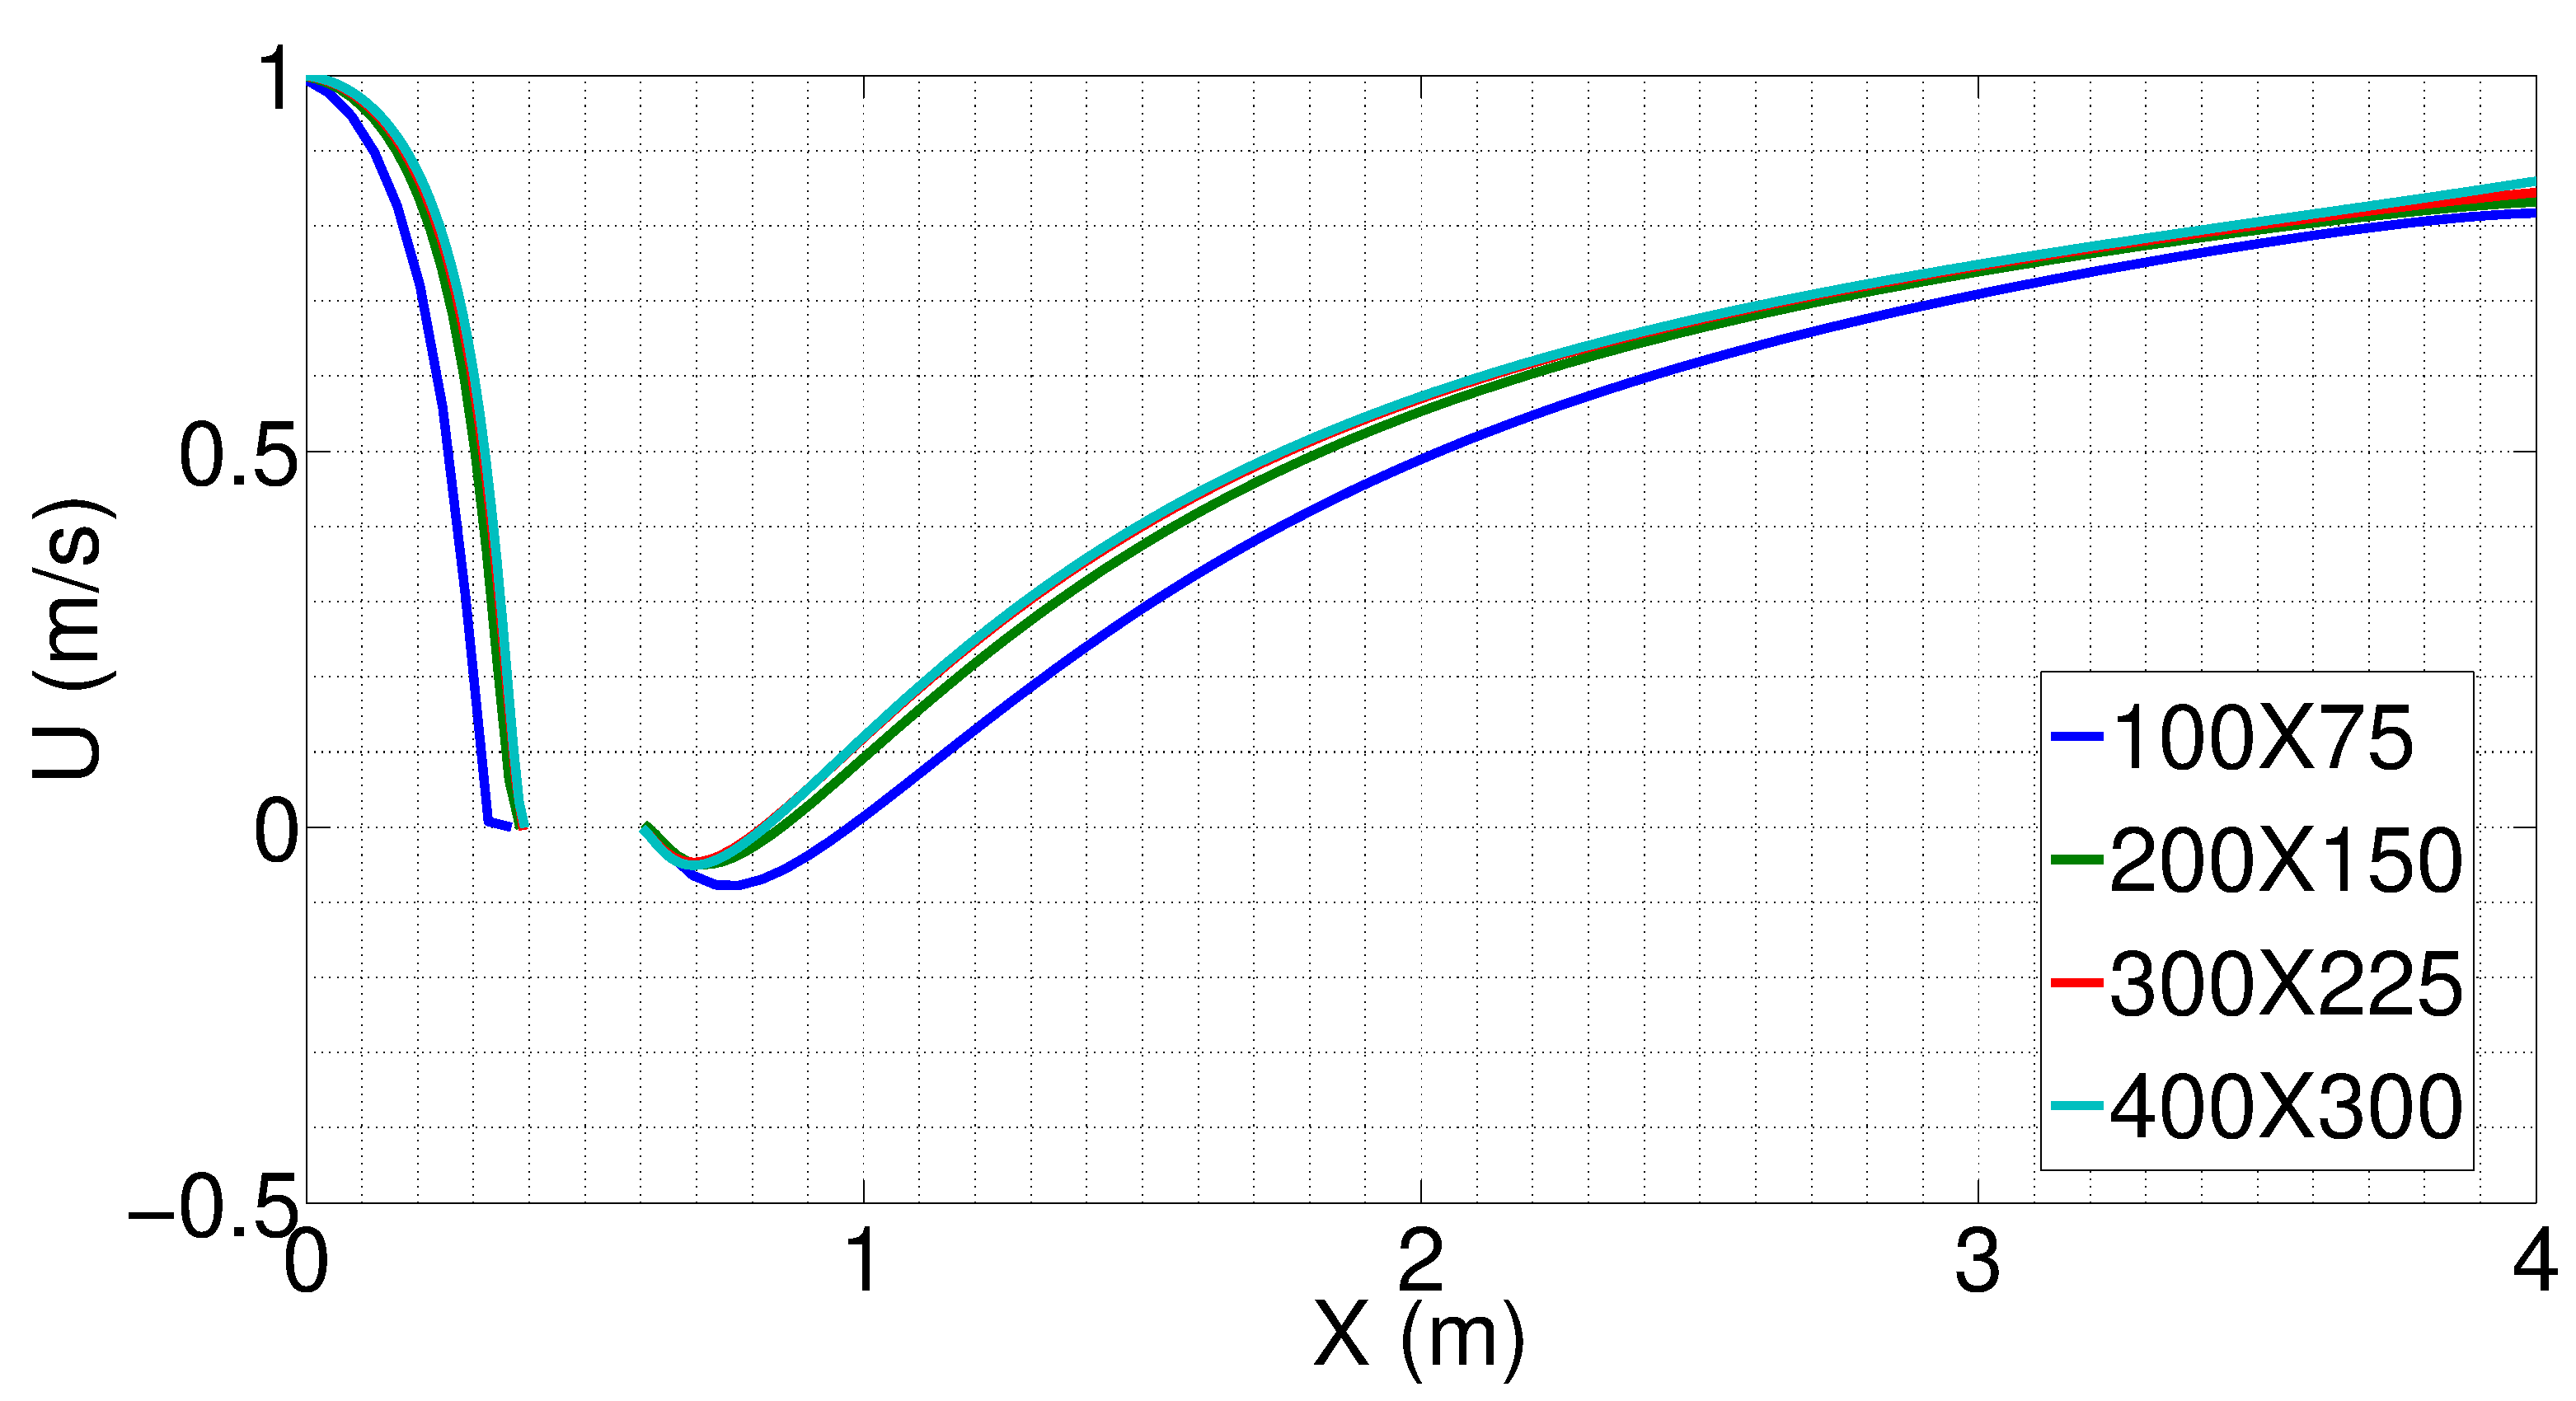
\includegraphics[width=7.0cm]{Chapter_4/figure/flow_over_cylinder/meshConvergence_RE100_U.eps}
    }
    \quad
    \subfigure[V-velocity on x = 0.5]
    {
    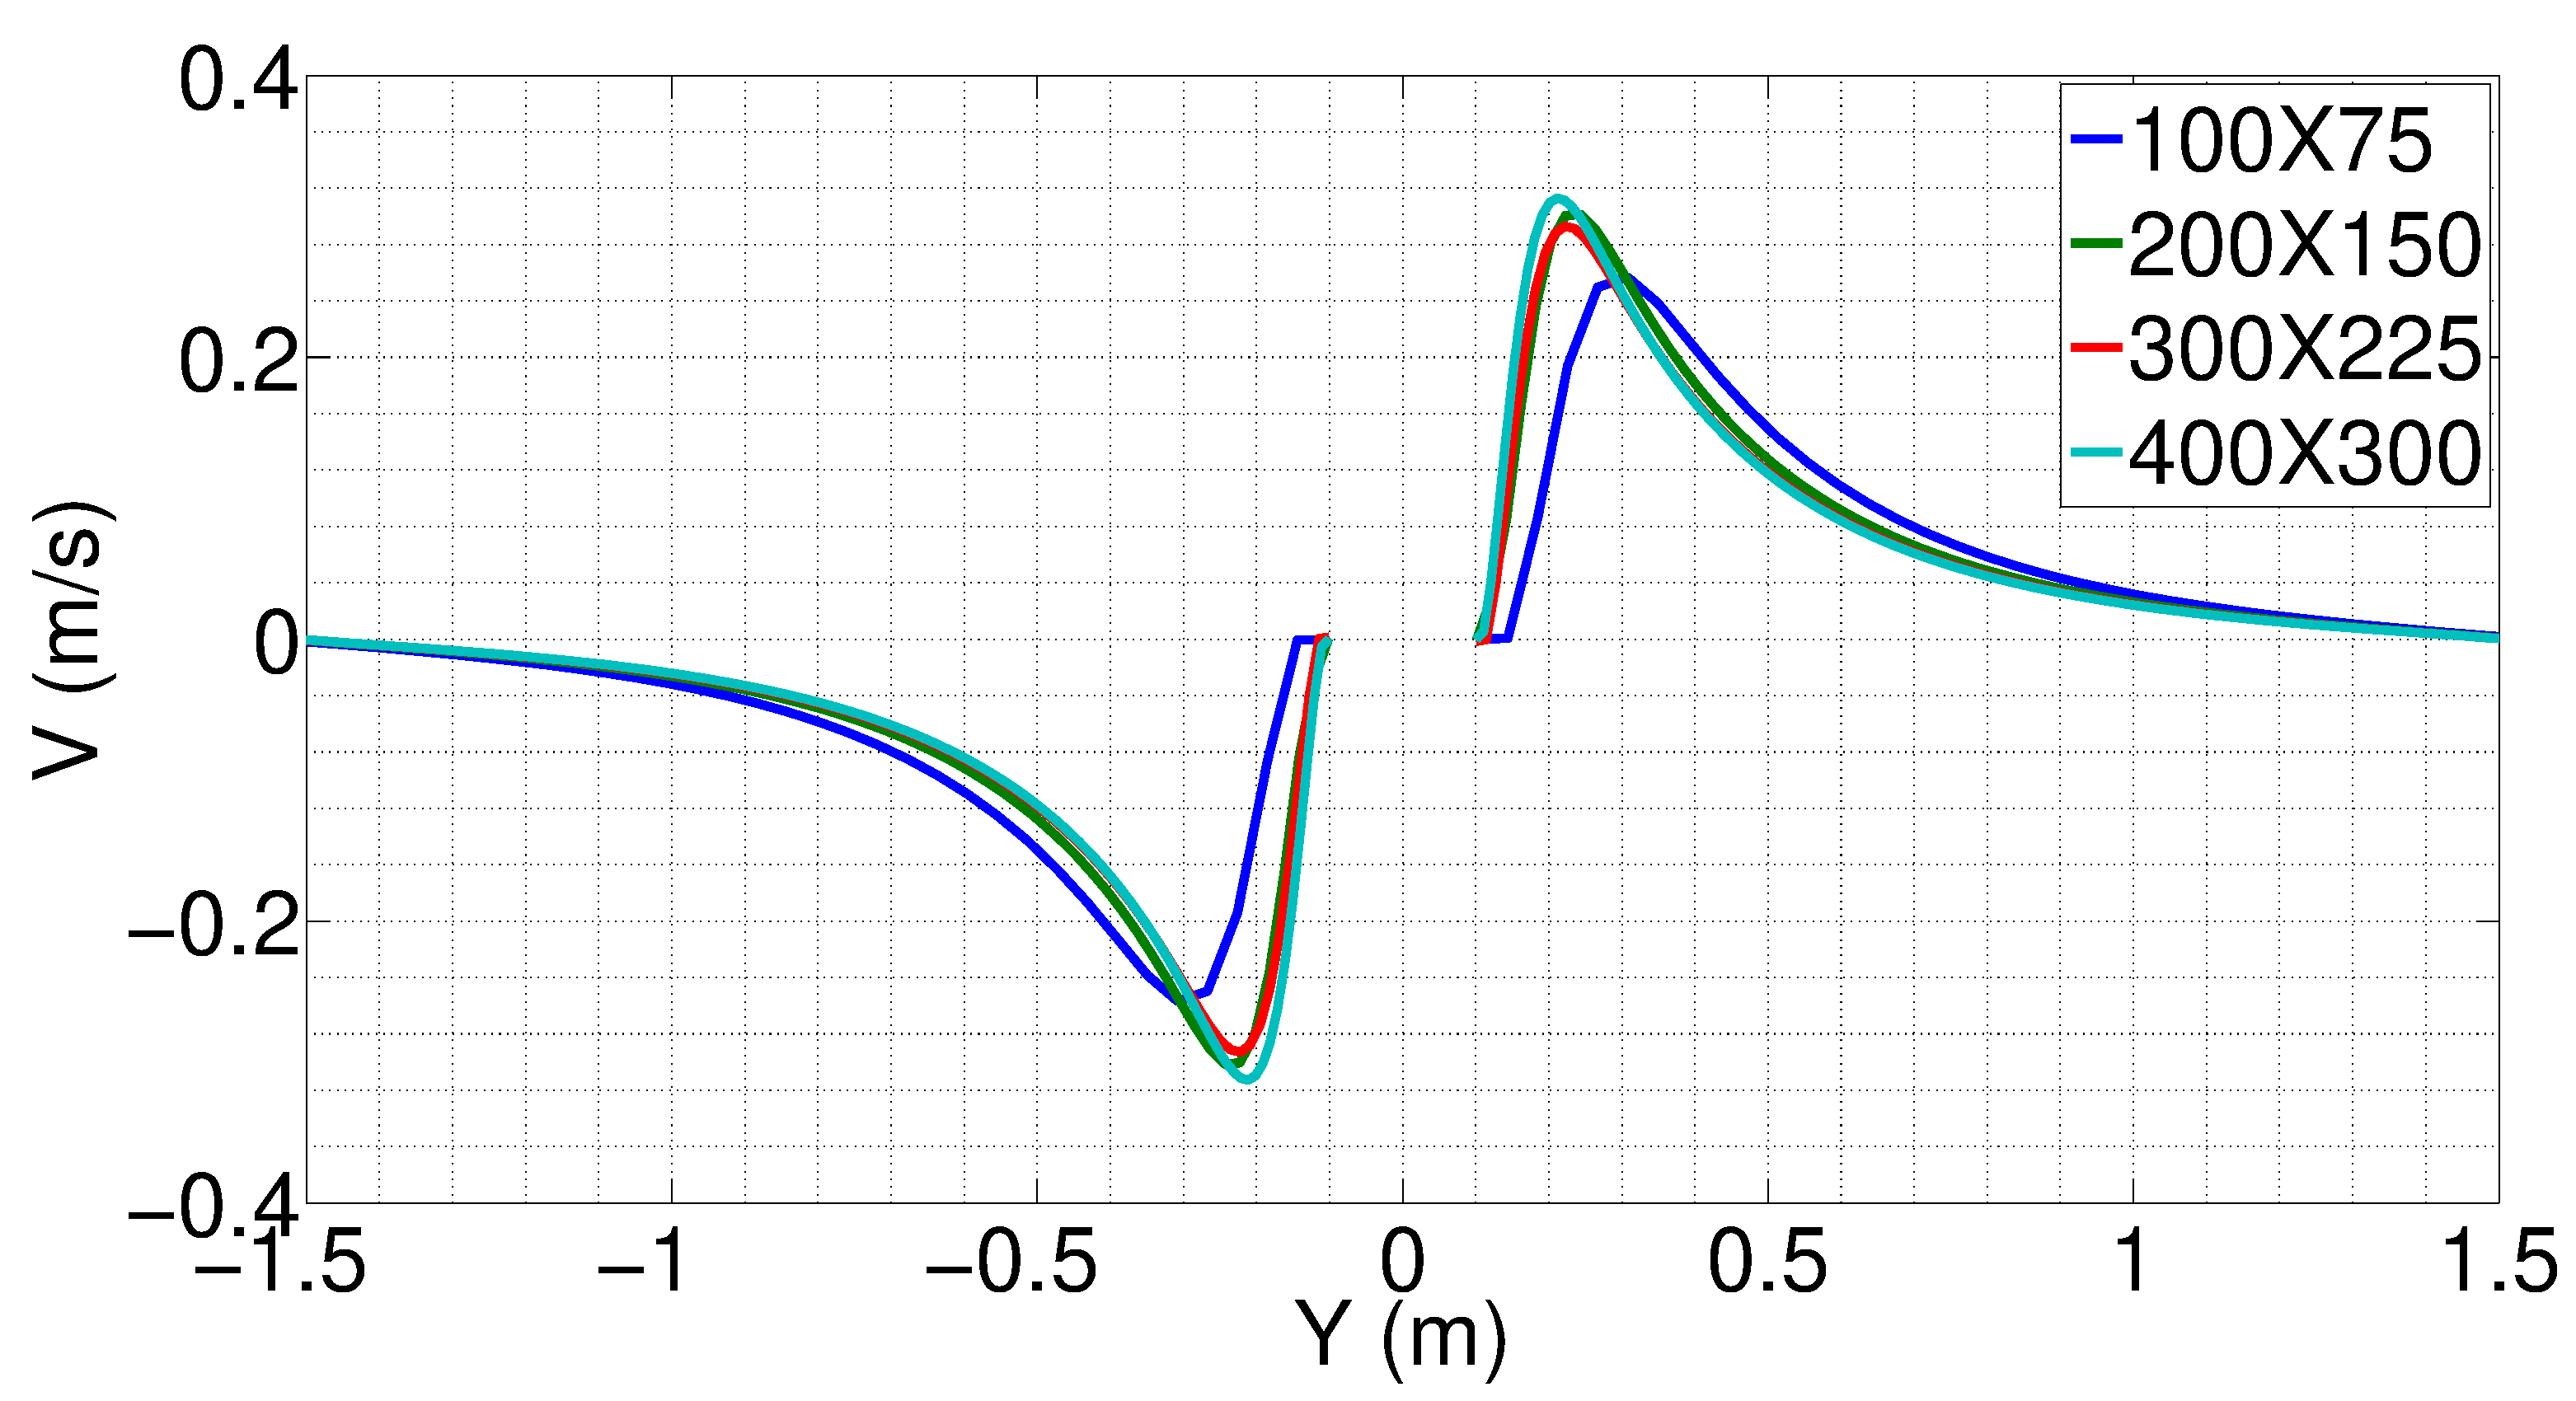
\includegraphics[width=7.0cm]{Chapter_4/figure/flow_over_cylinder/meshConvergence_RE100_V.eps}
    }
    \\
    \subfigure[Pressure on y = 0]
    {
    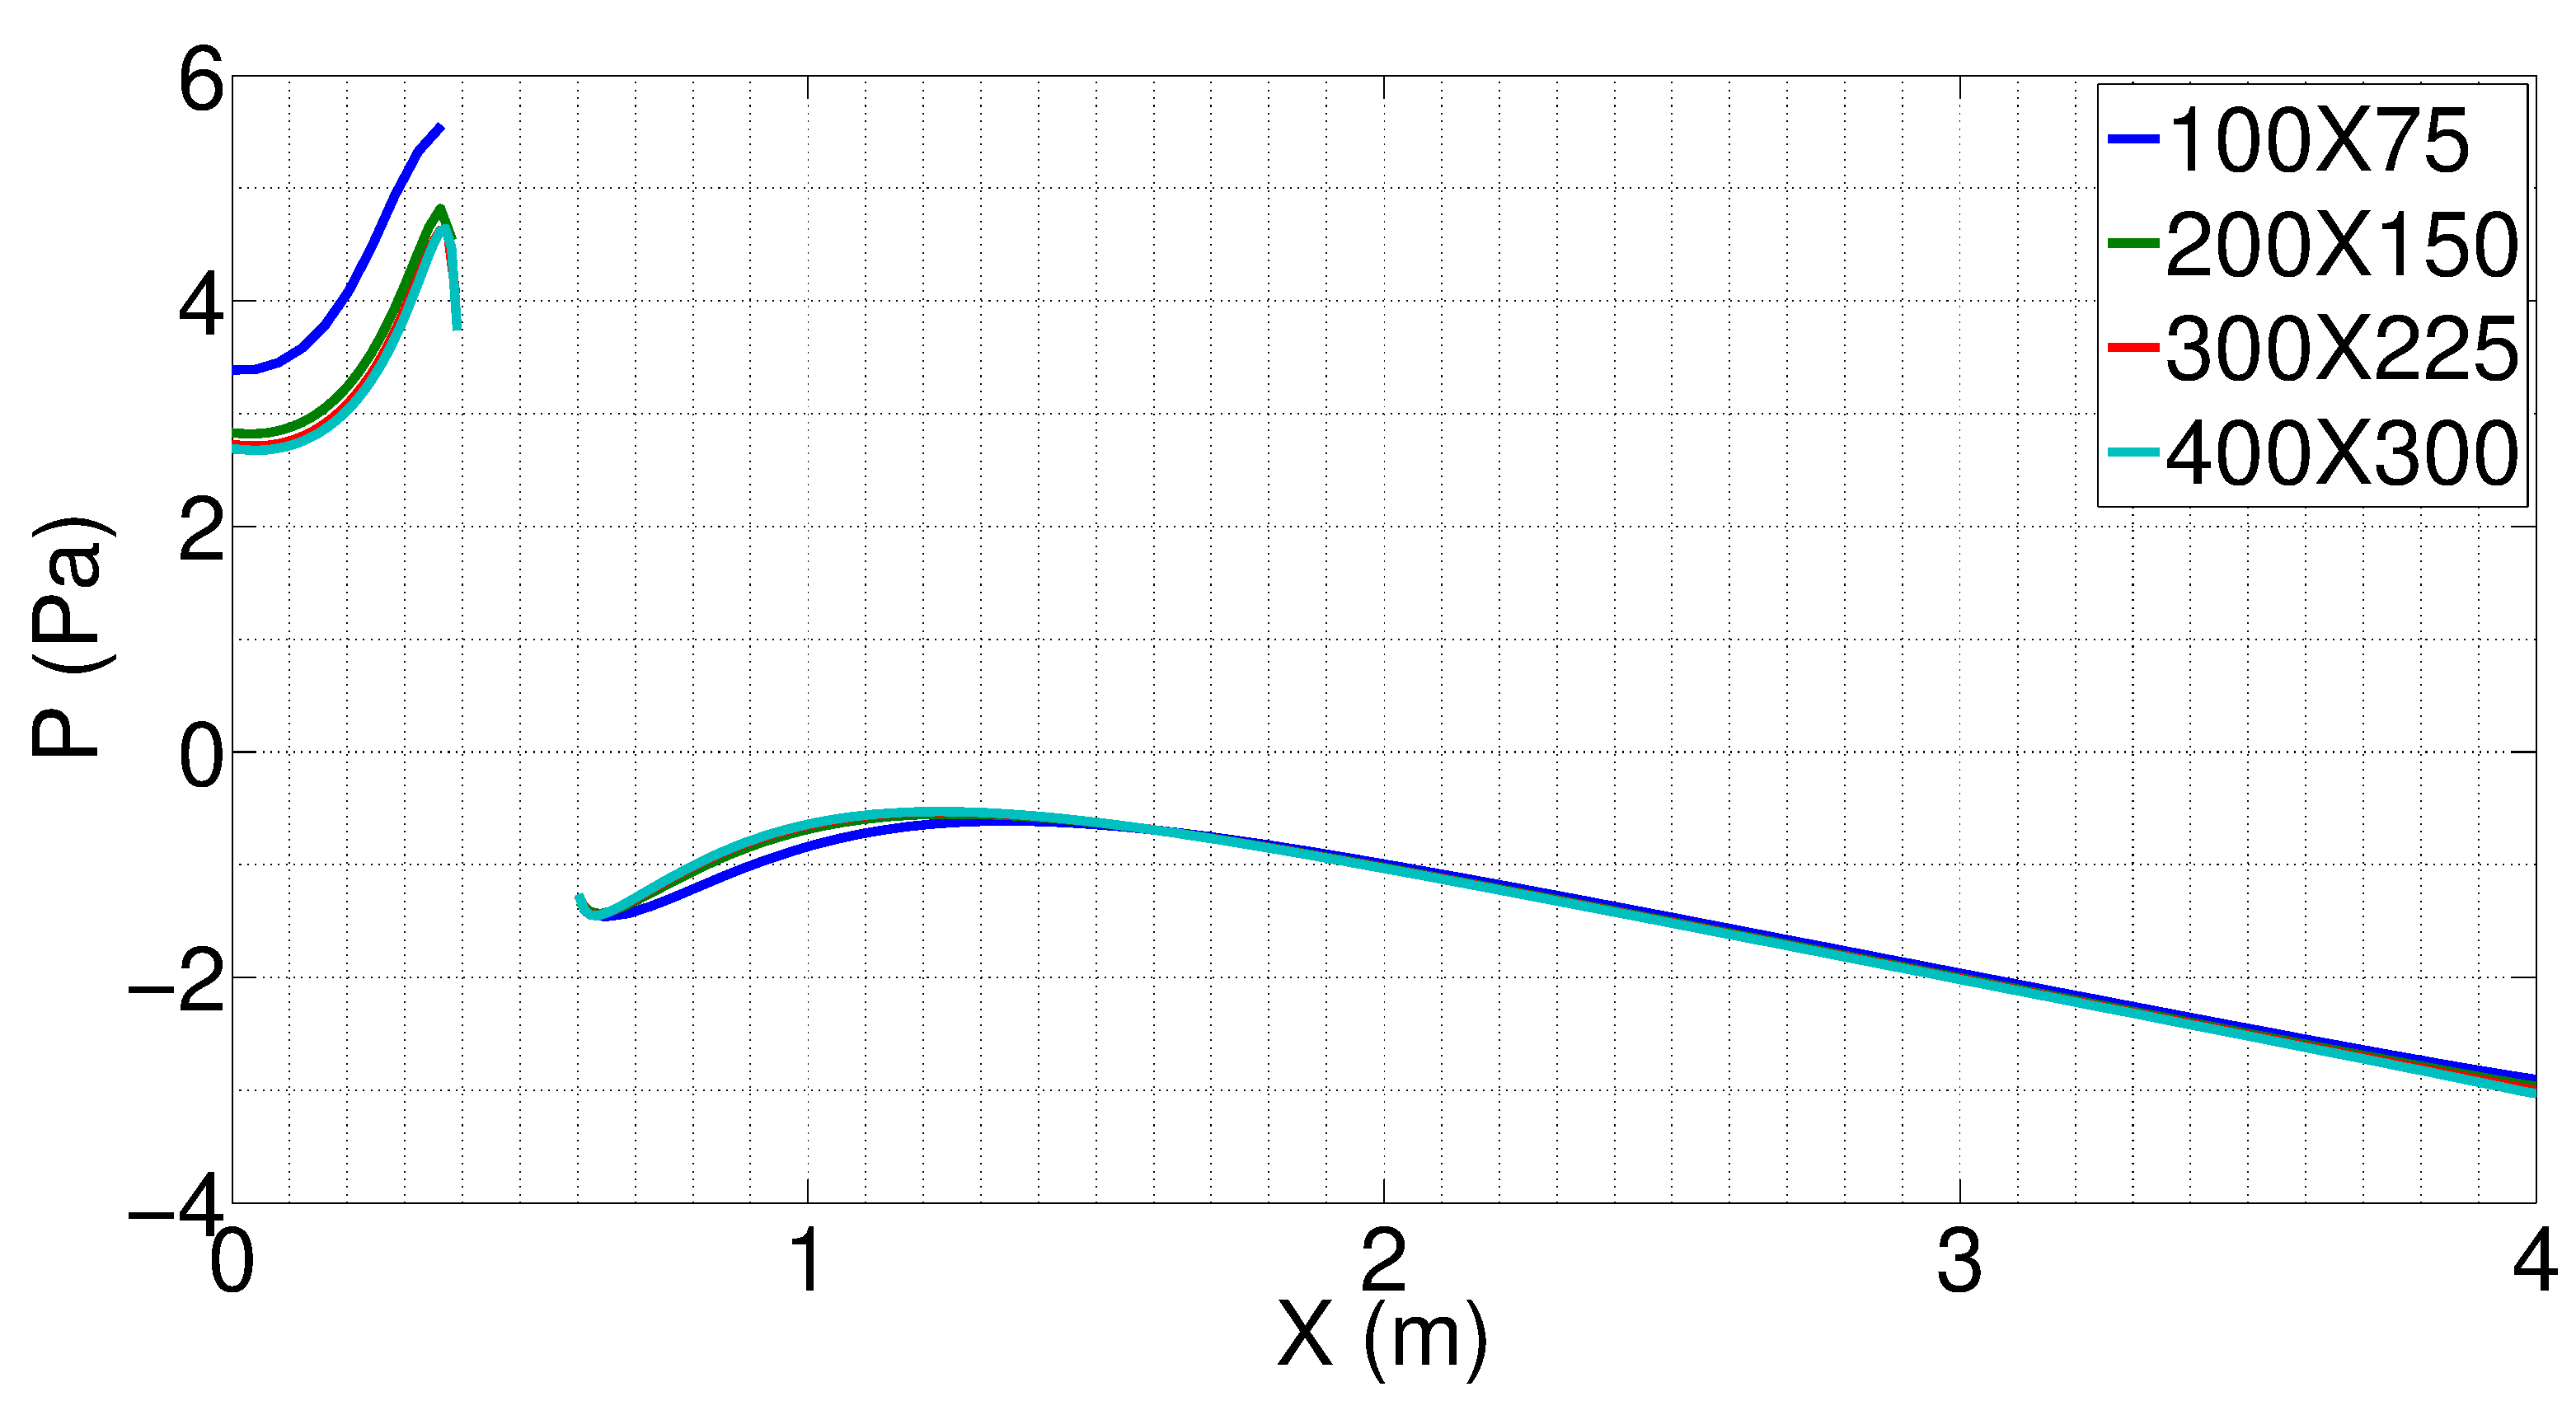
\includegraphics[width=7.0cm]{Chapter_4/figure/flow_over_cylinder/meshConvergence_RE100_P.eps}
    }
    \caption{Convergence results for Re = 100.}
    \label{fig:C4_meshConvergenceForCylidnerRE100GE}
\end{figure}

The convergence study of the mesh refinement is also conducted for a node on the downwash of the cylinder at $(2, 0)$ as shown in Figure \ref{fig:C4_meshRefinementForCylinderRE100GE}. The slopes of the fitted lines to the u-velocity, v-velocity, and pressure error estimates are calculated as $-2.34$, and $-1.96$, and $-2.72$. This means that the method is second order in space and time.

\begin{figure}[H]
    \centering
    \subfigure[U-velocity convergence on $(2.0, 0)$.]
    {
    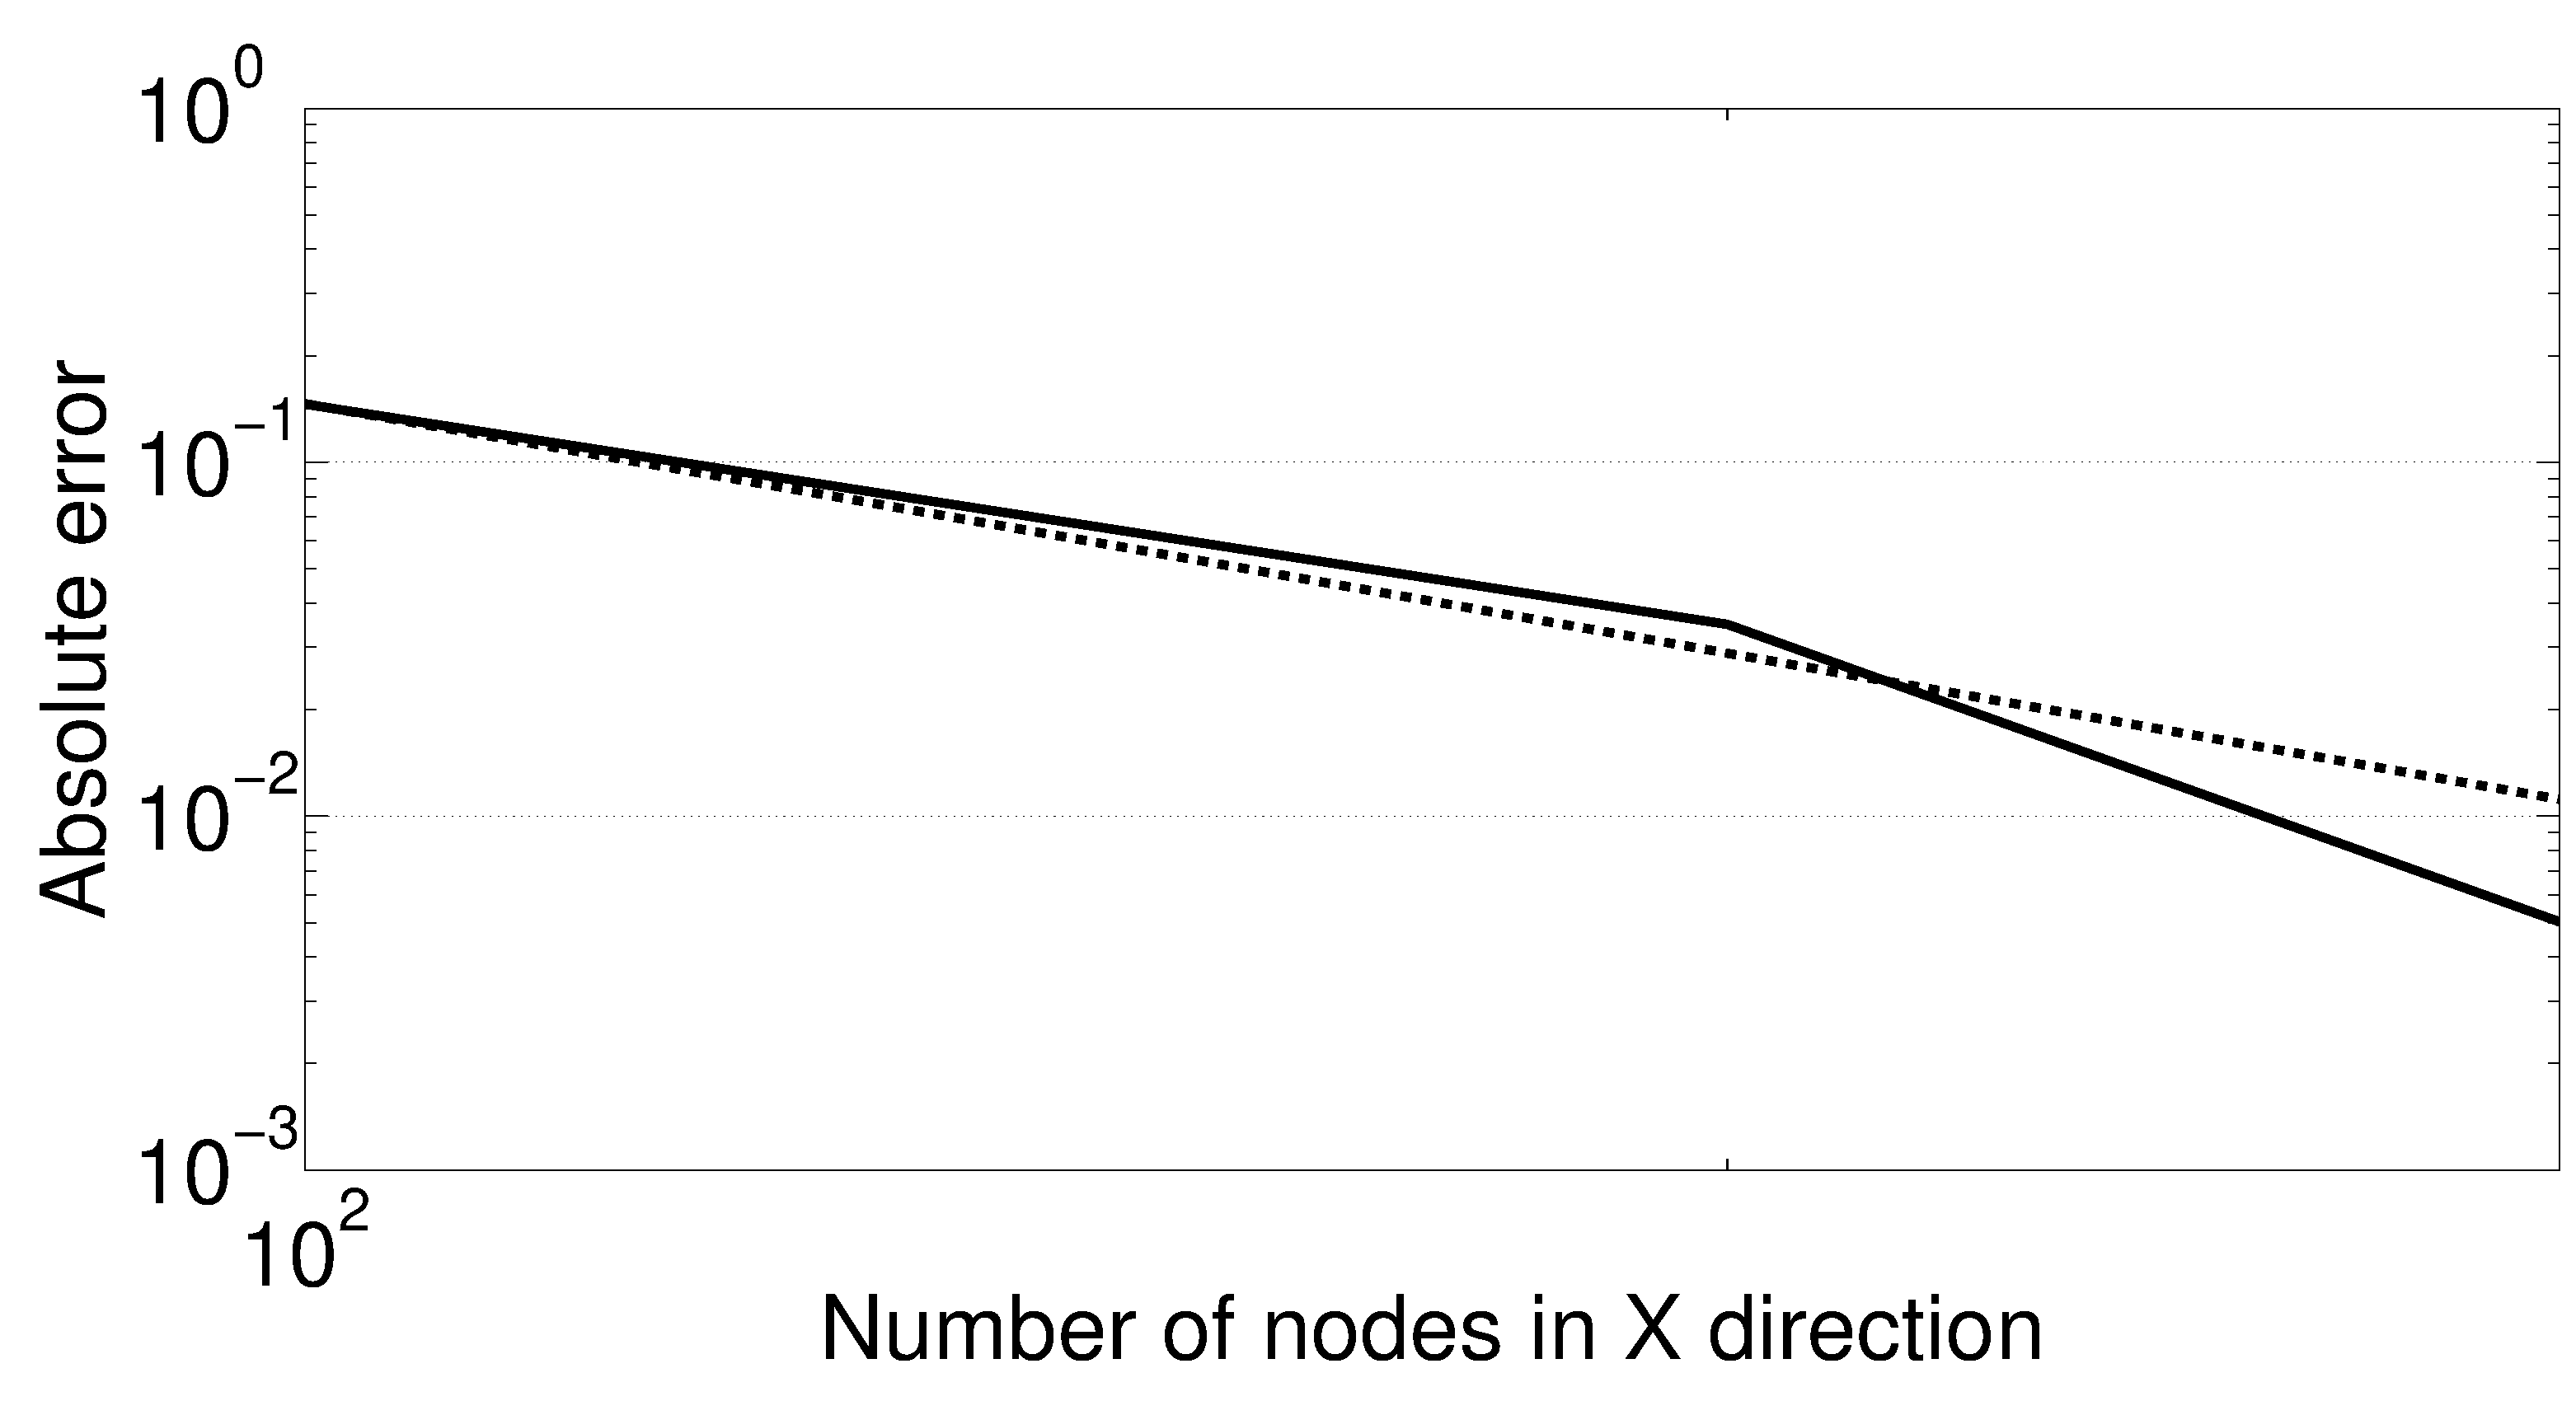
\includegraphics[width=7.0cm]{Chapter_4/figure/flow_over_cylinder/u_convergence_RE100.eps}
    }
    \quad
    \subfigure[V-velocity convergence on $(0.5, 0.75)$.]
    {
    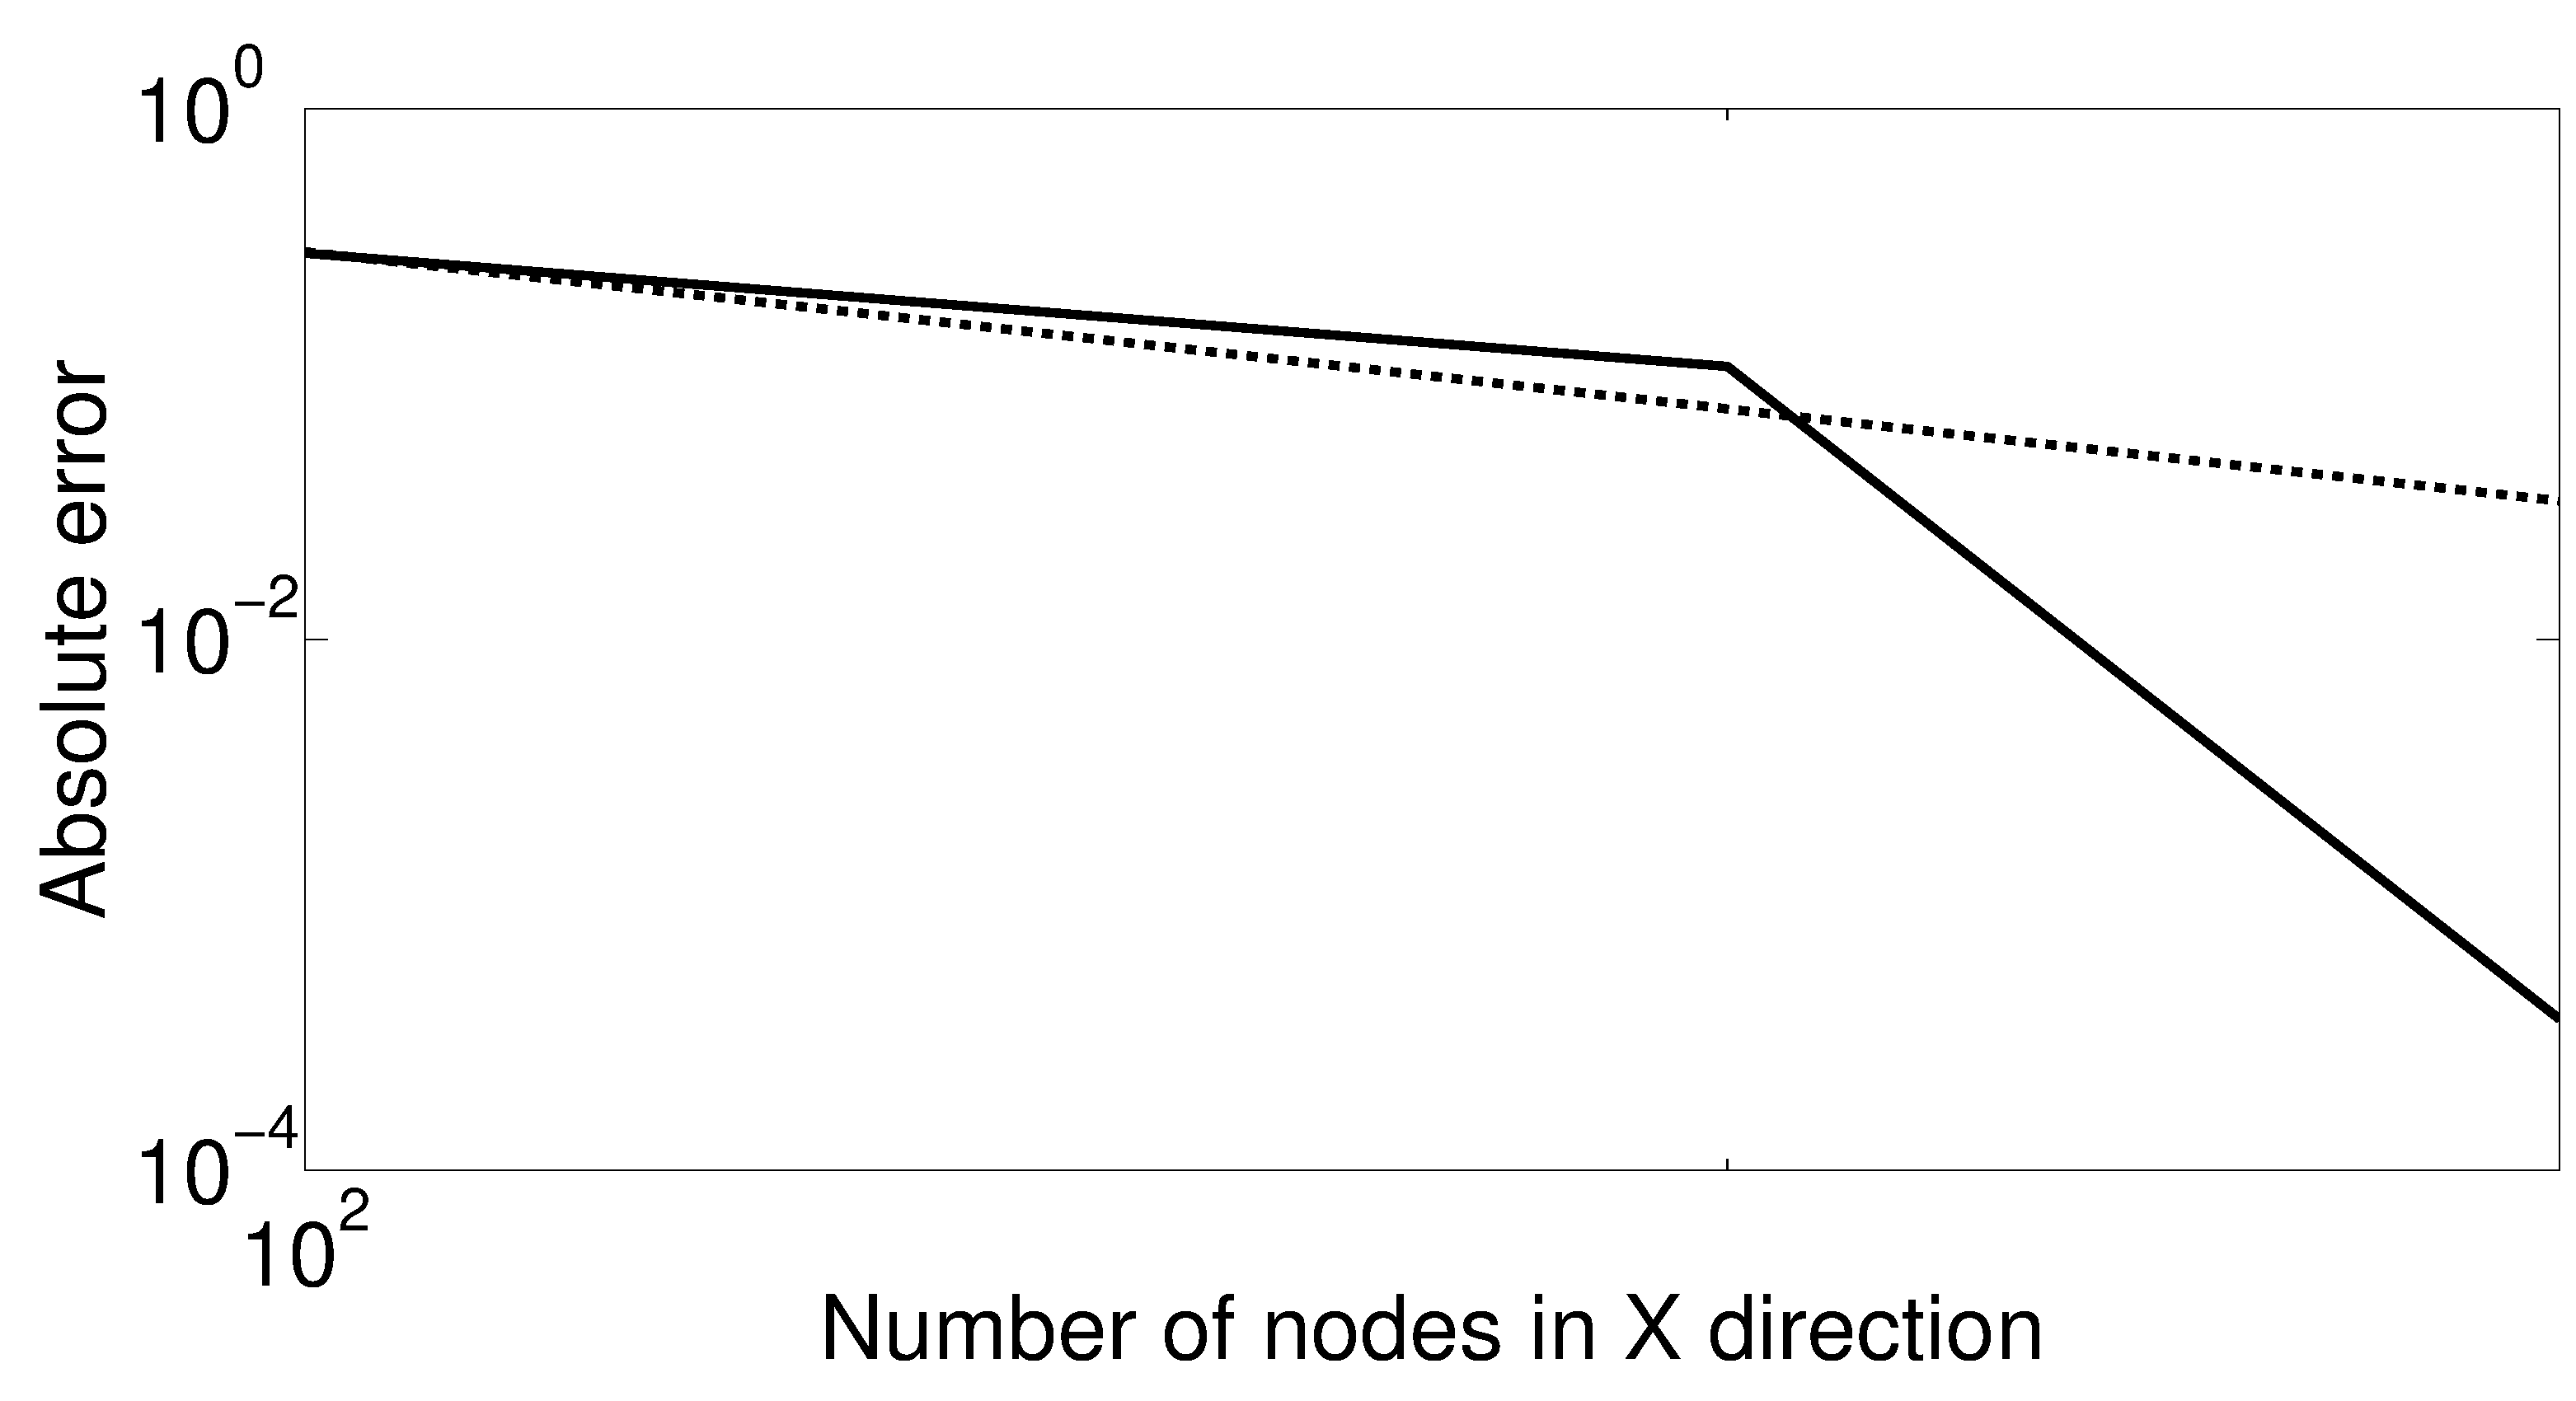
\includegraphics[width=7.0cm]{Chapter_4/figure/flow_over_cylinder/v_convergence_RE100.eps}
    }
    \\
    \subfigure[Pressure convergence on $(2.0, 0)$.]
    {
    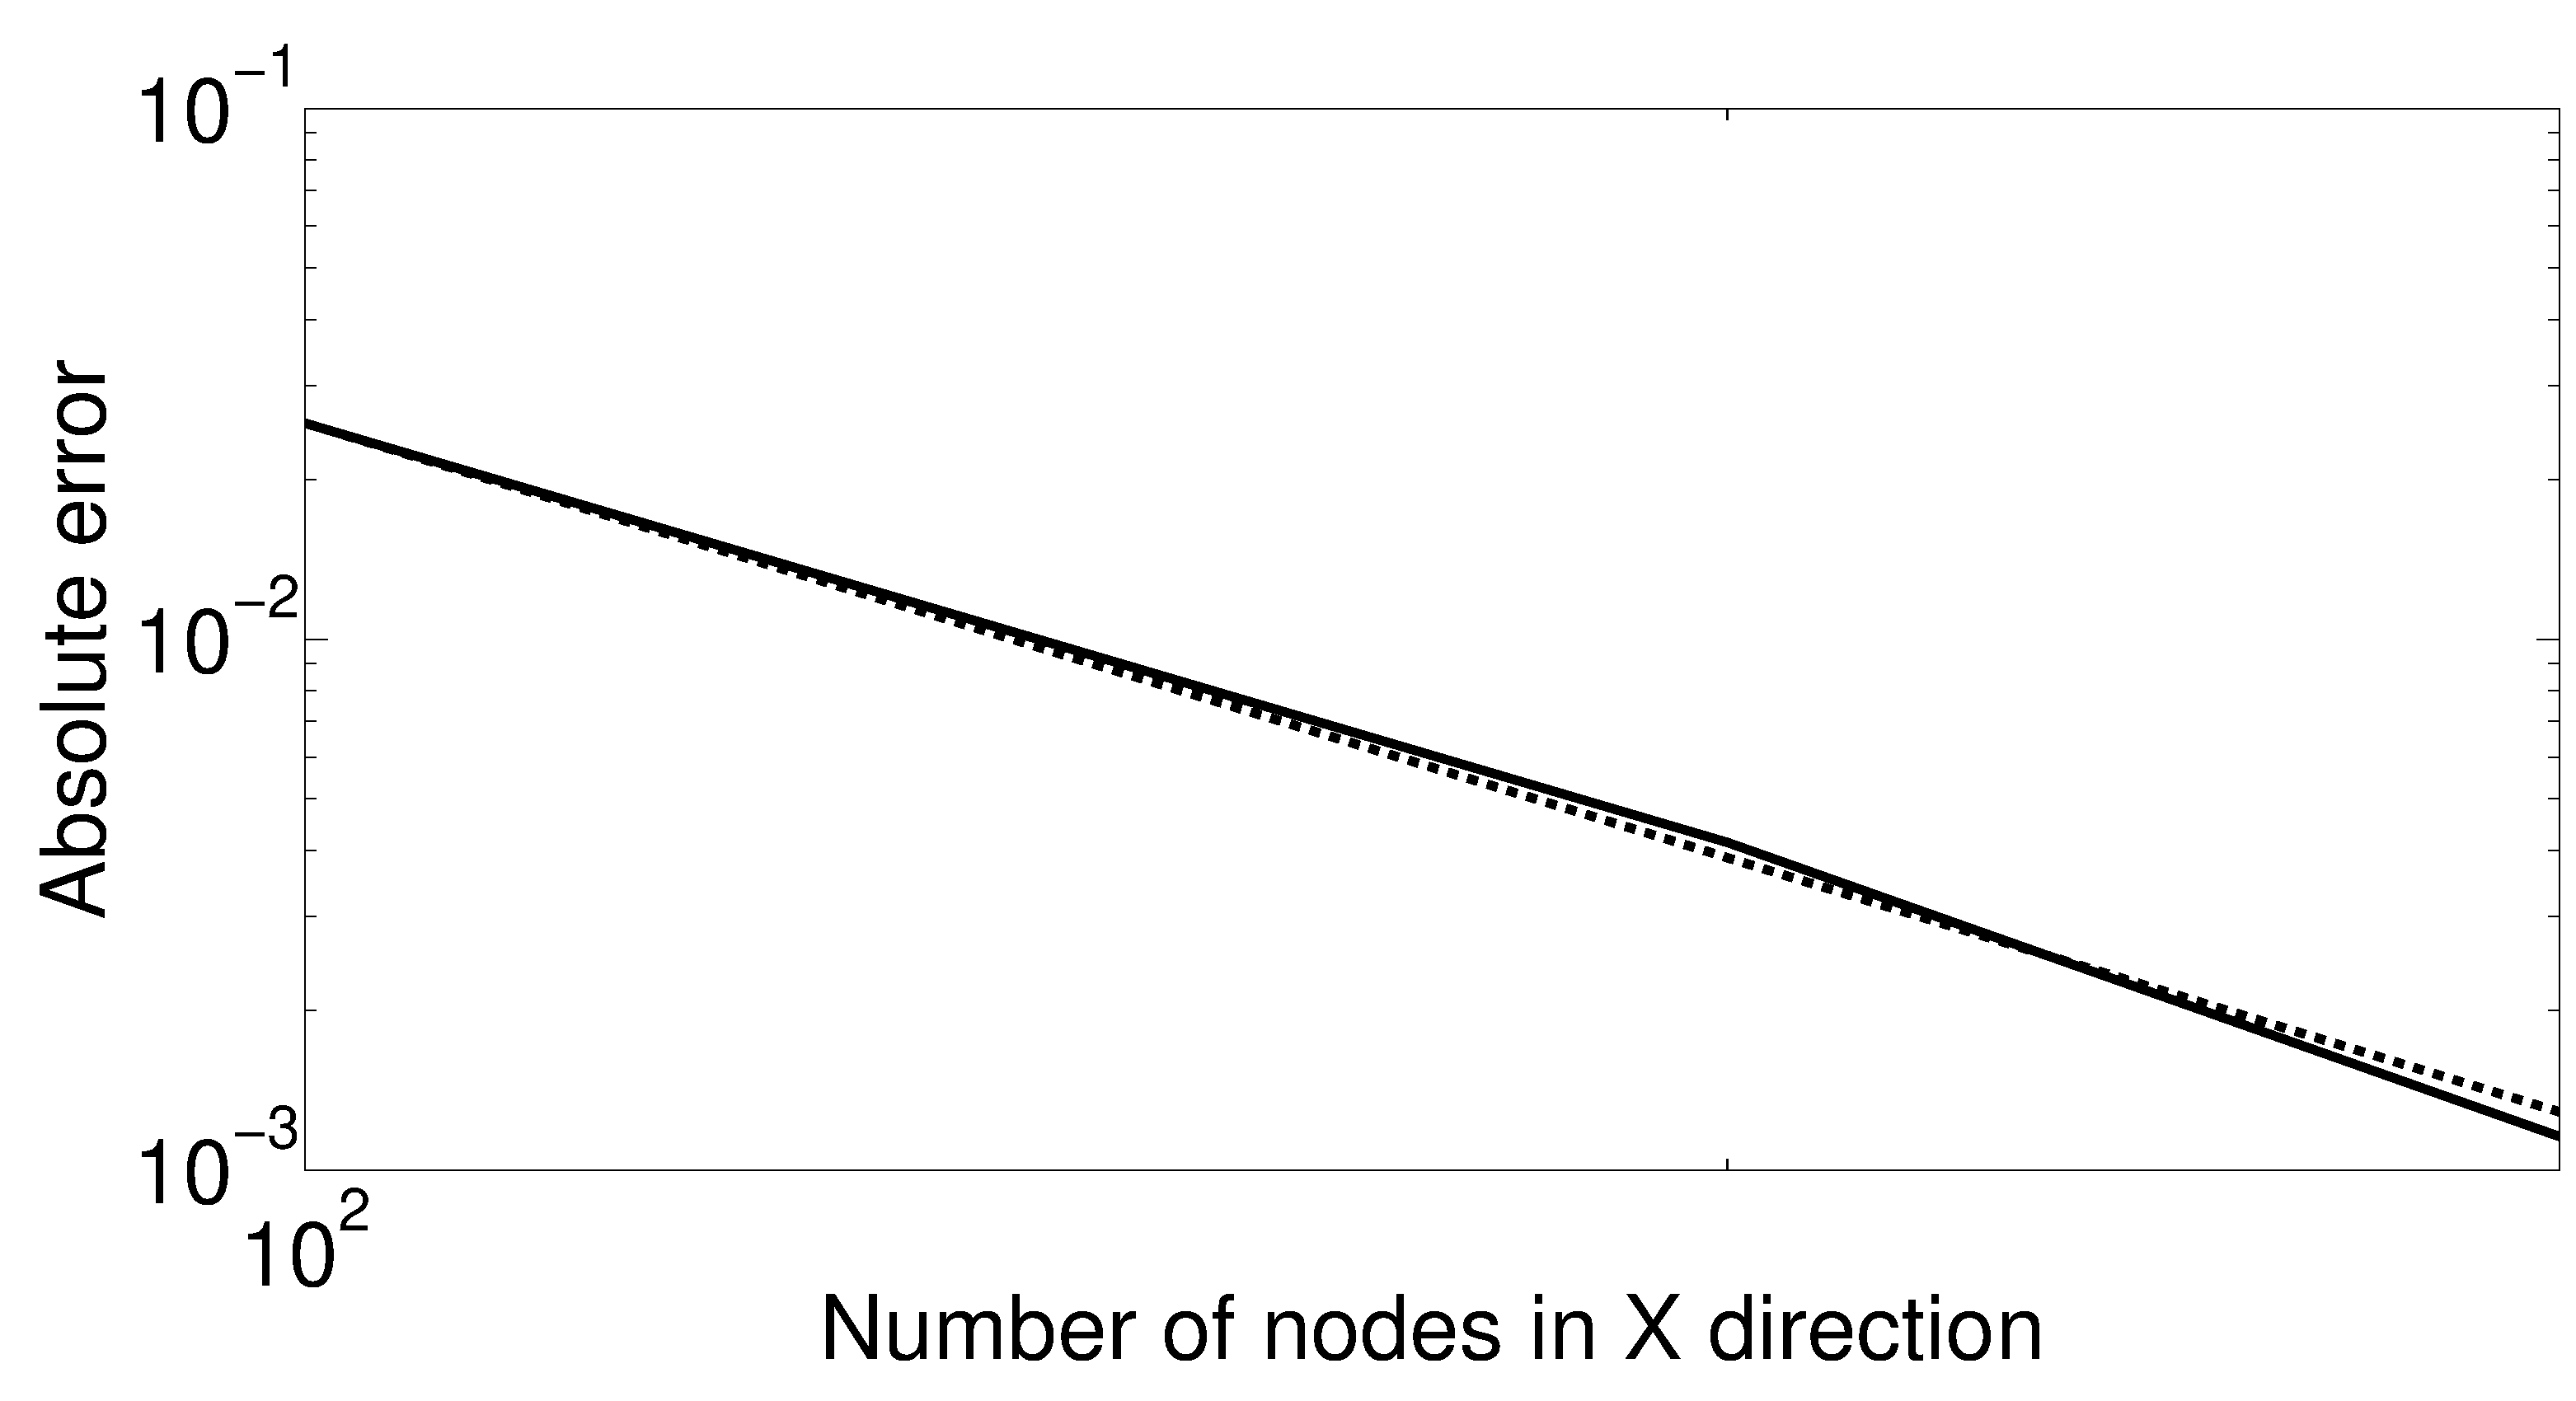
\includegraphics[width=7.0cm]{Chapter_4/figure/flow_over_cylinder/pressure_convergence_RE100.eps}
    }
    \caption{Convergence plots for Re = 100.}
    \label{fig:C4_meshRefinementForCylinderRE100GE}
\end{figure}

The contour plots for the velocity and pressure is shown in Figure \ref{fig:contourPlotsForFlowOverCylidnerGE}.

\begin{figure}[H]
    \centering
    \subfigure[U-velocity]
    {
    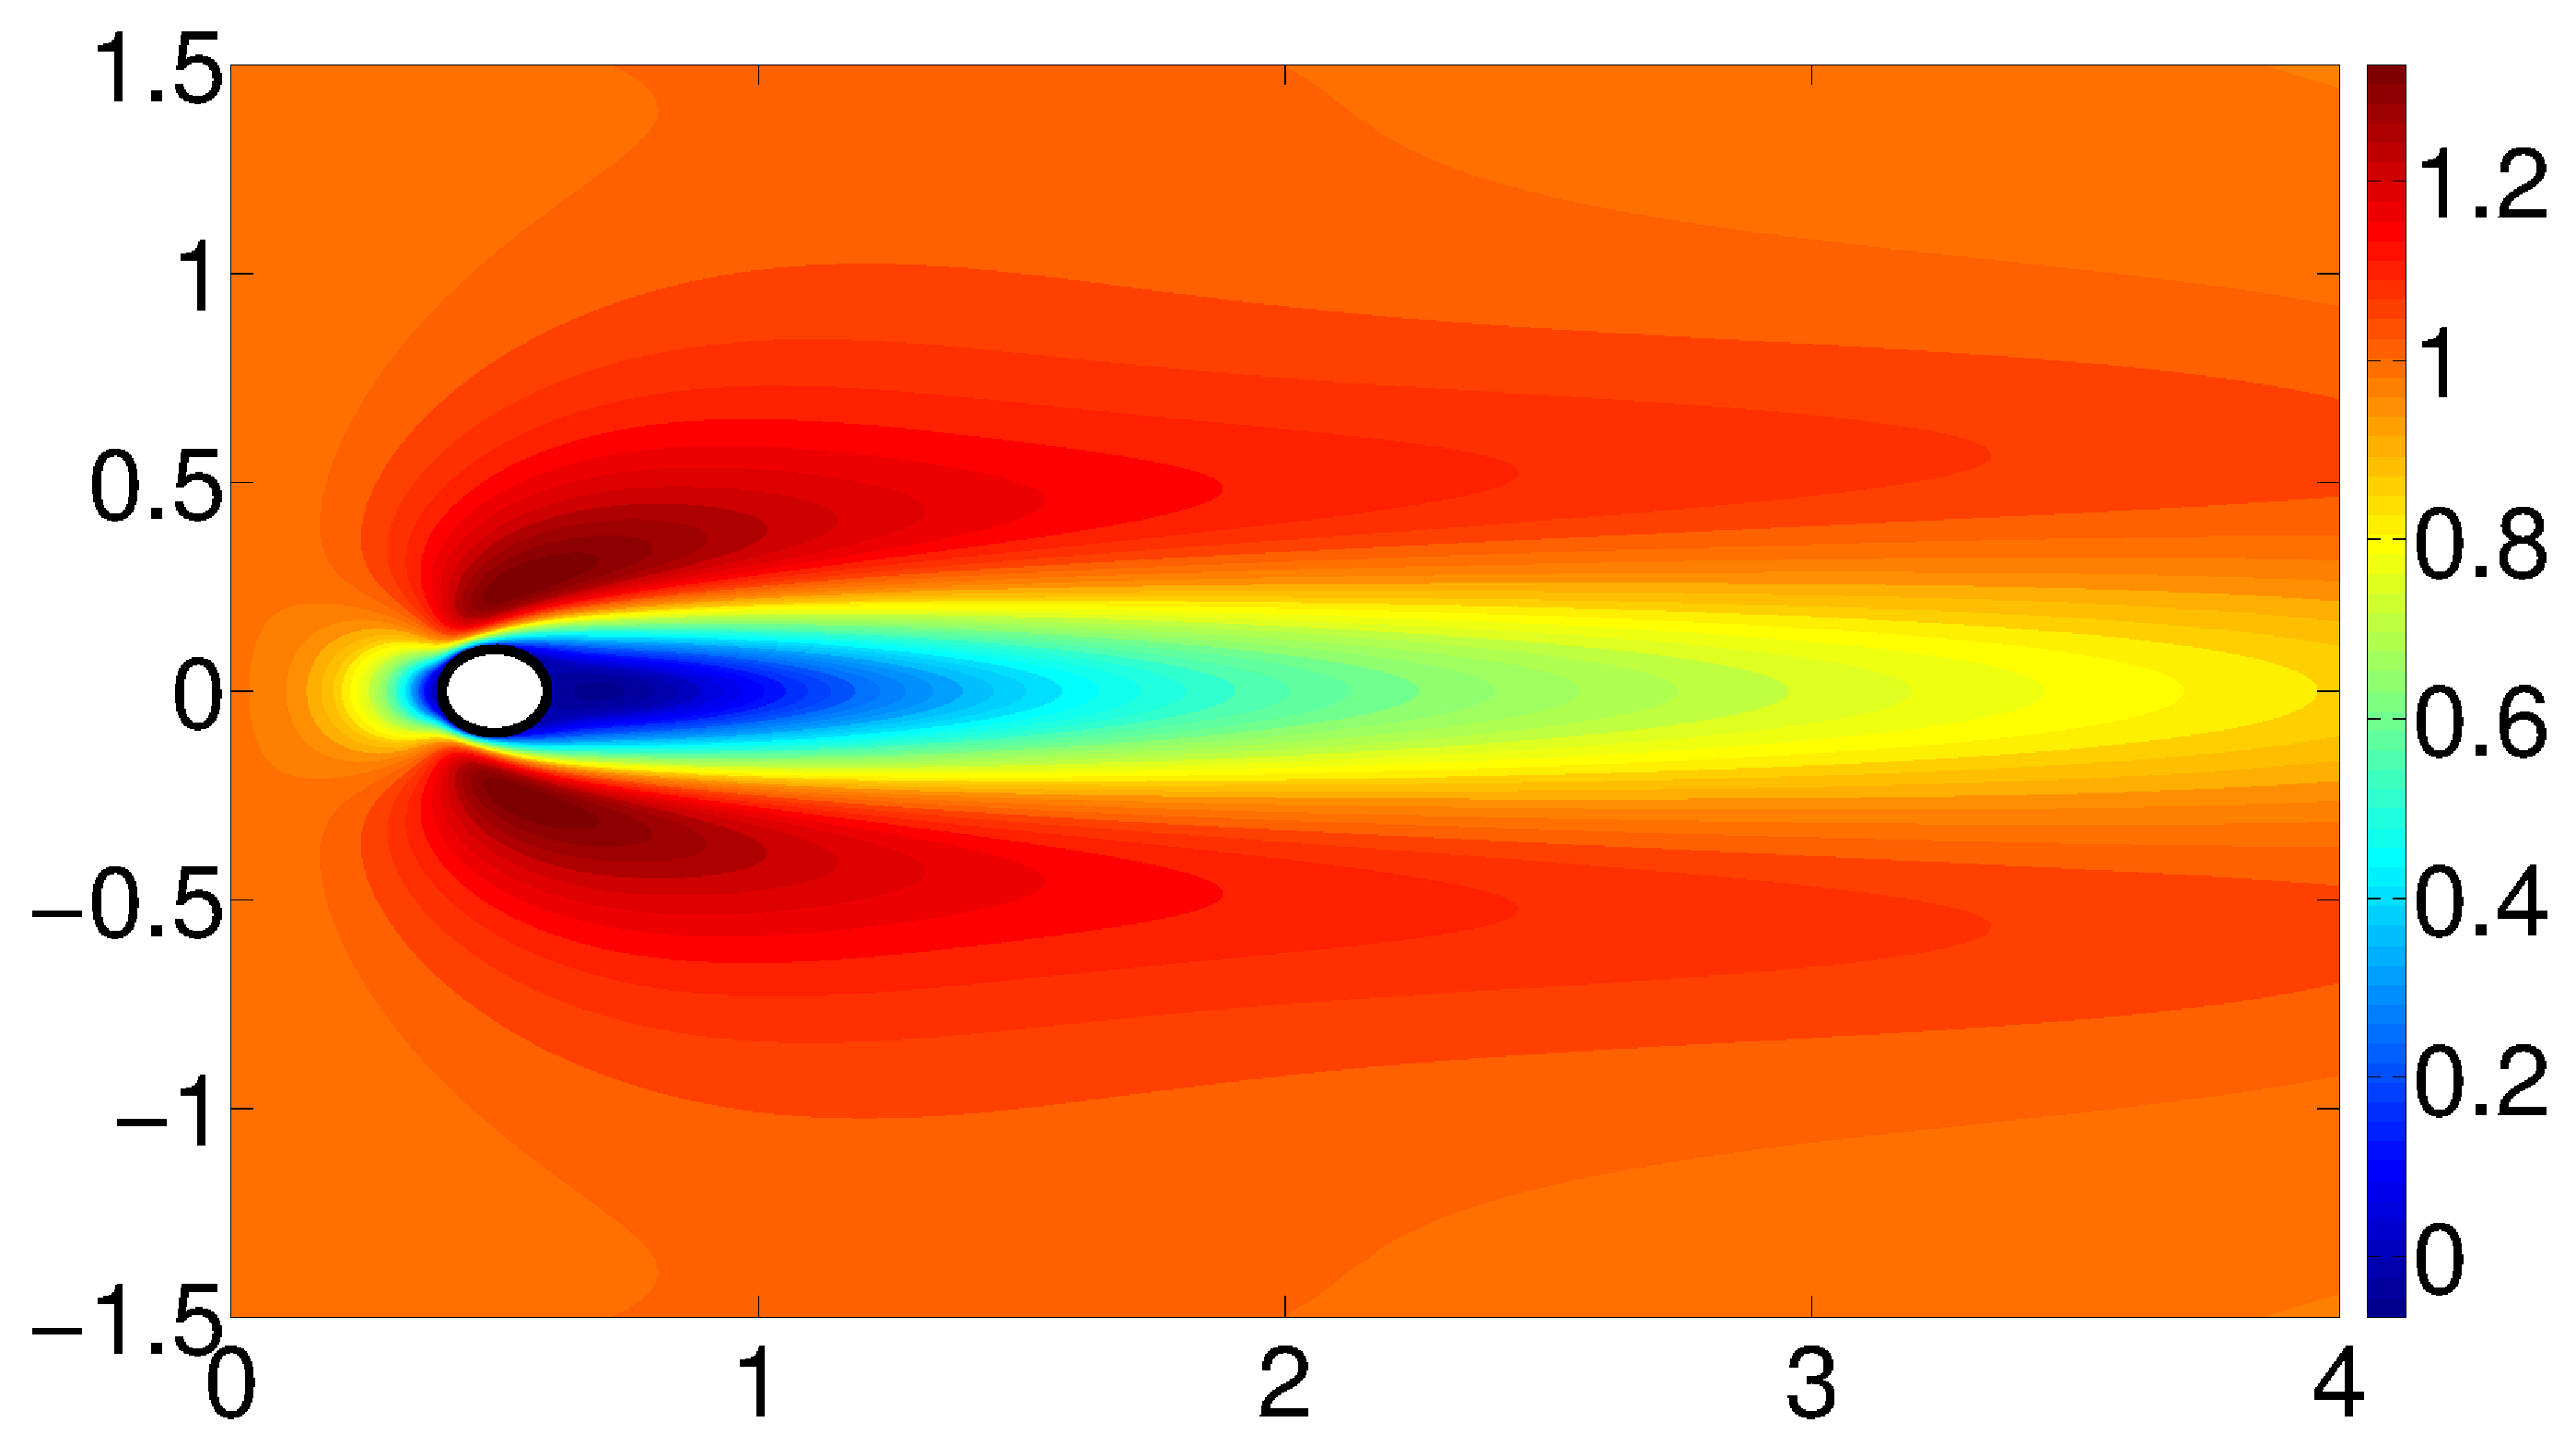
\includegraphics[width=7.0cm]{Chapter_4/figure/flow_over_cylinder/u_velocity_contour_RE100.eps}
    }
    \quad
    \subfigure[V-velocity]
    {
    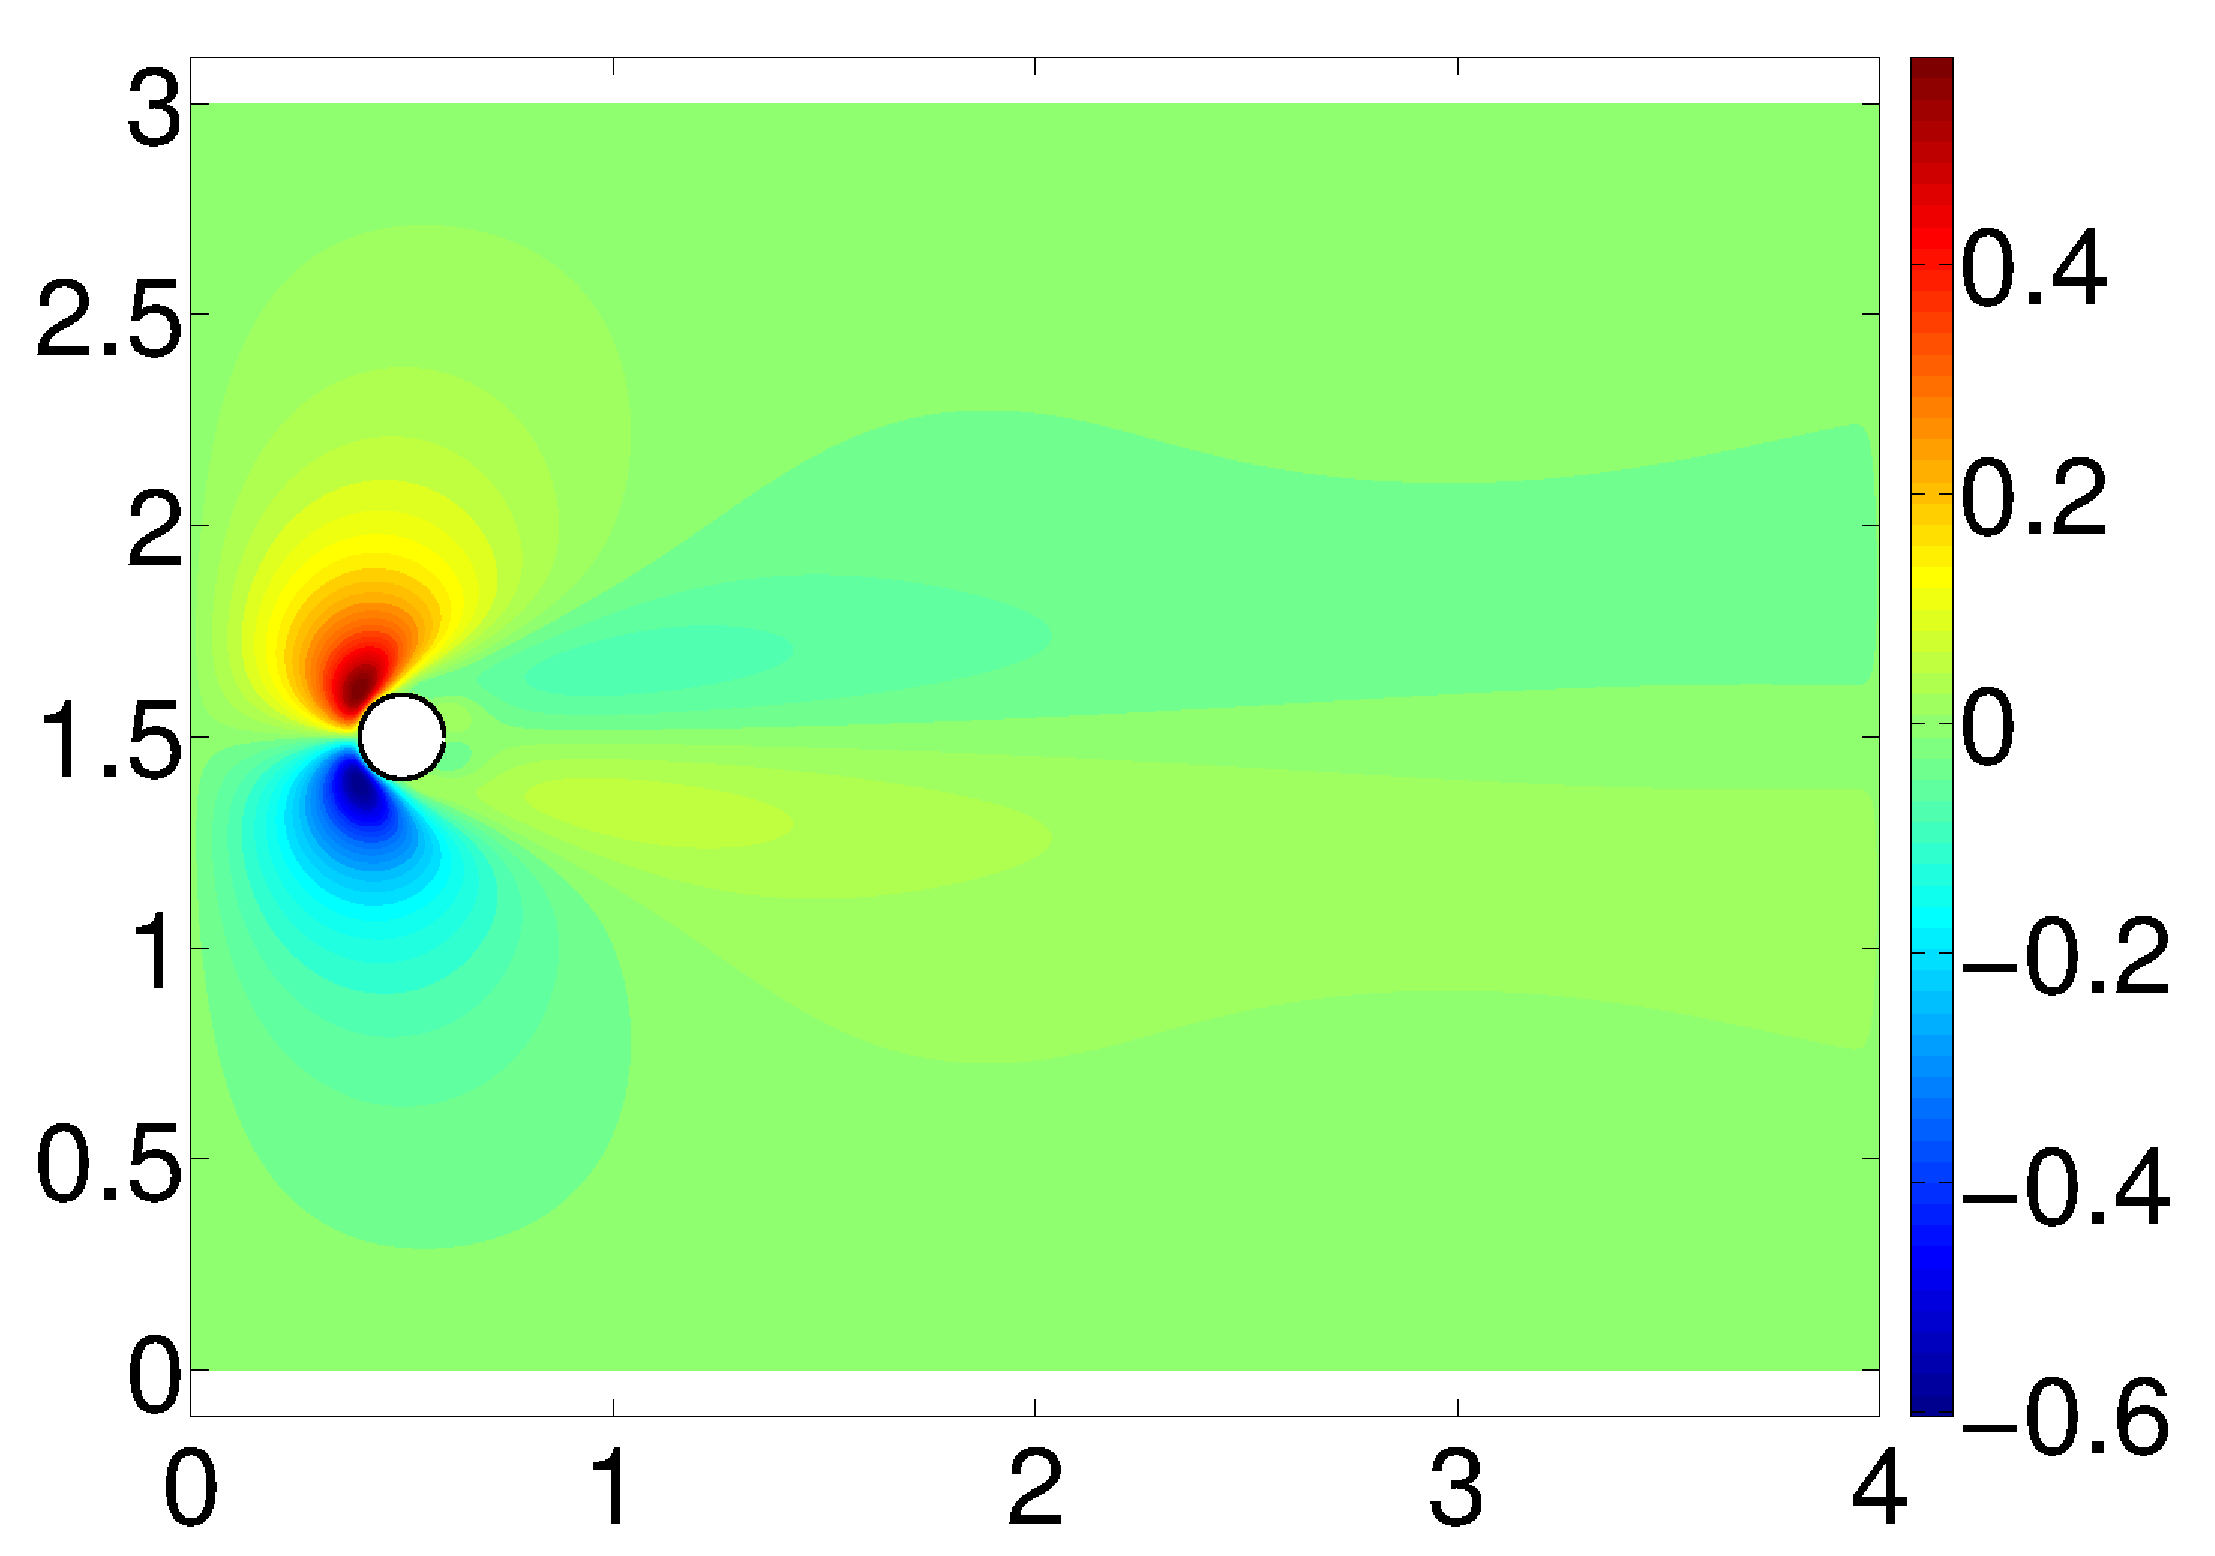
\includegraphics[width=7.0cm]{Chapter_4/figure/flow_over_cylinder/v_velocity_contour_RE100.eps}
    }
    \caption{Velocity contours for Re = 100.}
    \label{fig:contourPlotsForFlowOverCylidnerGE}
\end{figure}

To ensure that the zero velocity on the solid boundary, we looked at the value of the u and v velocities at the Lagrangian points on the boundary.
% ======================================================================
\section{Shape Sensitivity of Flow through a Nozzle}
In this section, the flow in a convergent-divergent nozzle is modeled using the virtual boundary method and the sensitivity of flow with respect to the change of the shape of the nozzle is calculated.  The shape of the nozzle is defined using three points: inlet, throat, and outlet. The inlet and outlet points are represented as red circles, while a red cross represents the throat point in Figure \ref{fig:C4_nozzleShape}. The shape of the nozzle is approximated as a second-order polynomial passing through the point at the inlet and the throat node and separate second-order polynomial connecting throat and the outlet node. To ensure a smooth shape for the nozzle, the polynomials are forced to have zero derivatives at the throat. The throat area is controlled by the relative distance of the throat node from the symmetry line of the nozzle, $y_t$. This is selected as the design variable for sensitivity analysis. The analytical equation of the nozzle's top wall in terms of the design variable, $y_t$, is written as
%
\begin{equation}
	y(x) = 
	\begin{cases}
		(0.61 - 2.04 y_t)x^2 + (1.22y_t - 0.36) x + (0.81y_t + 0.55) \quad &\text{if} \quad 0.0 \leq x \leq 0.3 \\
		(3.34 - 11.11 y_t)x^2 + (6.67y_t - 2.0)x + 0.8 \quad &\text{if} \quad 0.3 < x \leq 1.0
	\end{cases}
\end{equation}
%
The bottom wall formula can be found by mirroring the top equation with respect to the symmetry line, $y = 0.5$.

The shape of the nozzle for different design variables are shown in Figure \ref{fig:C4_nozzleShape}
%
\begin{figure}[H]
    \centering
    \subfigure[Nozzle shape for $y_t = 0.1$.]
    {
    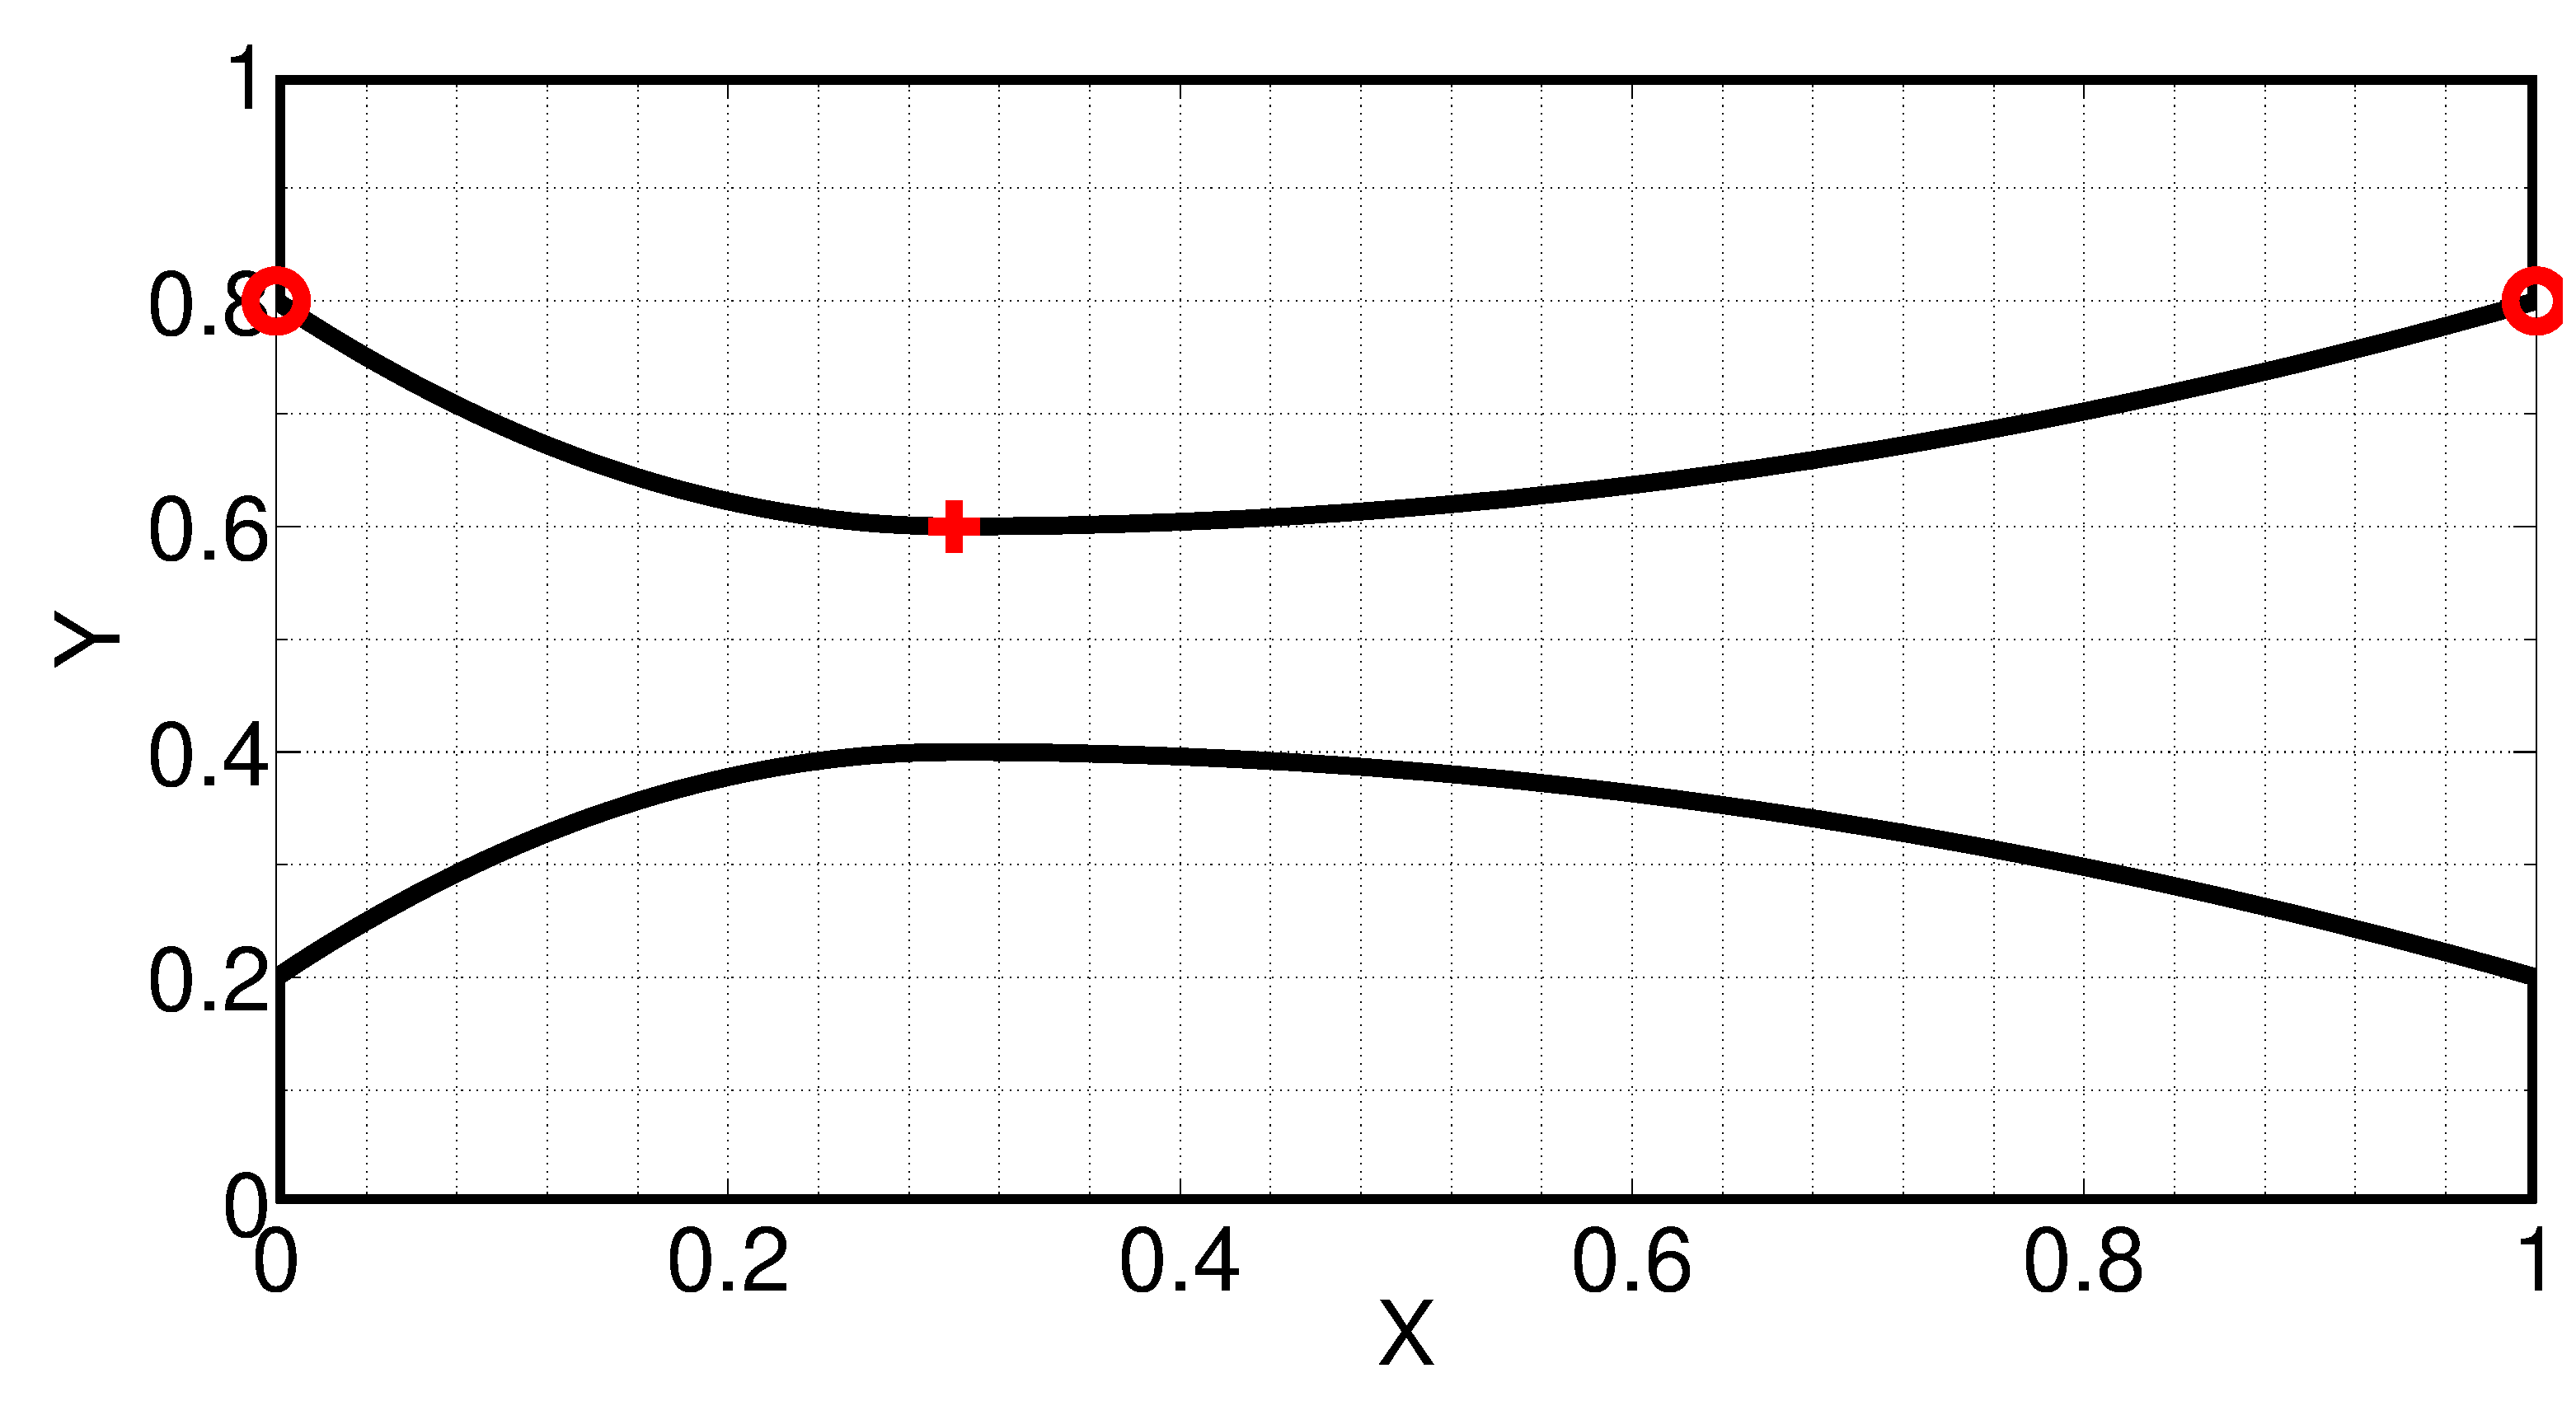
\includegraphics[width=6.5cm]{Chapter_4/figure/flow_through_nozzle/nozzle_shape_yt01.eps}
    }
    \quad
    \subfigure[Nozzle shape for $y_t = 0.2$]
    {
    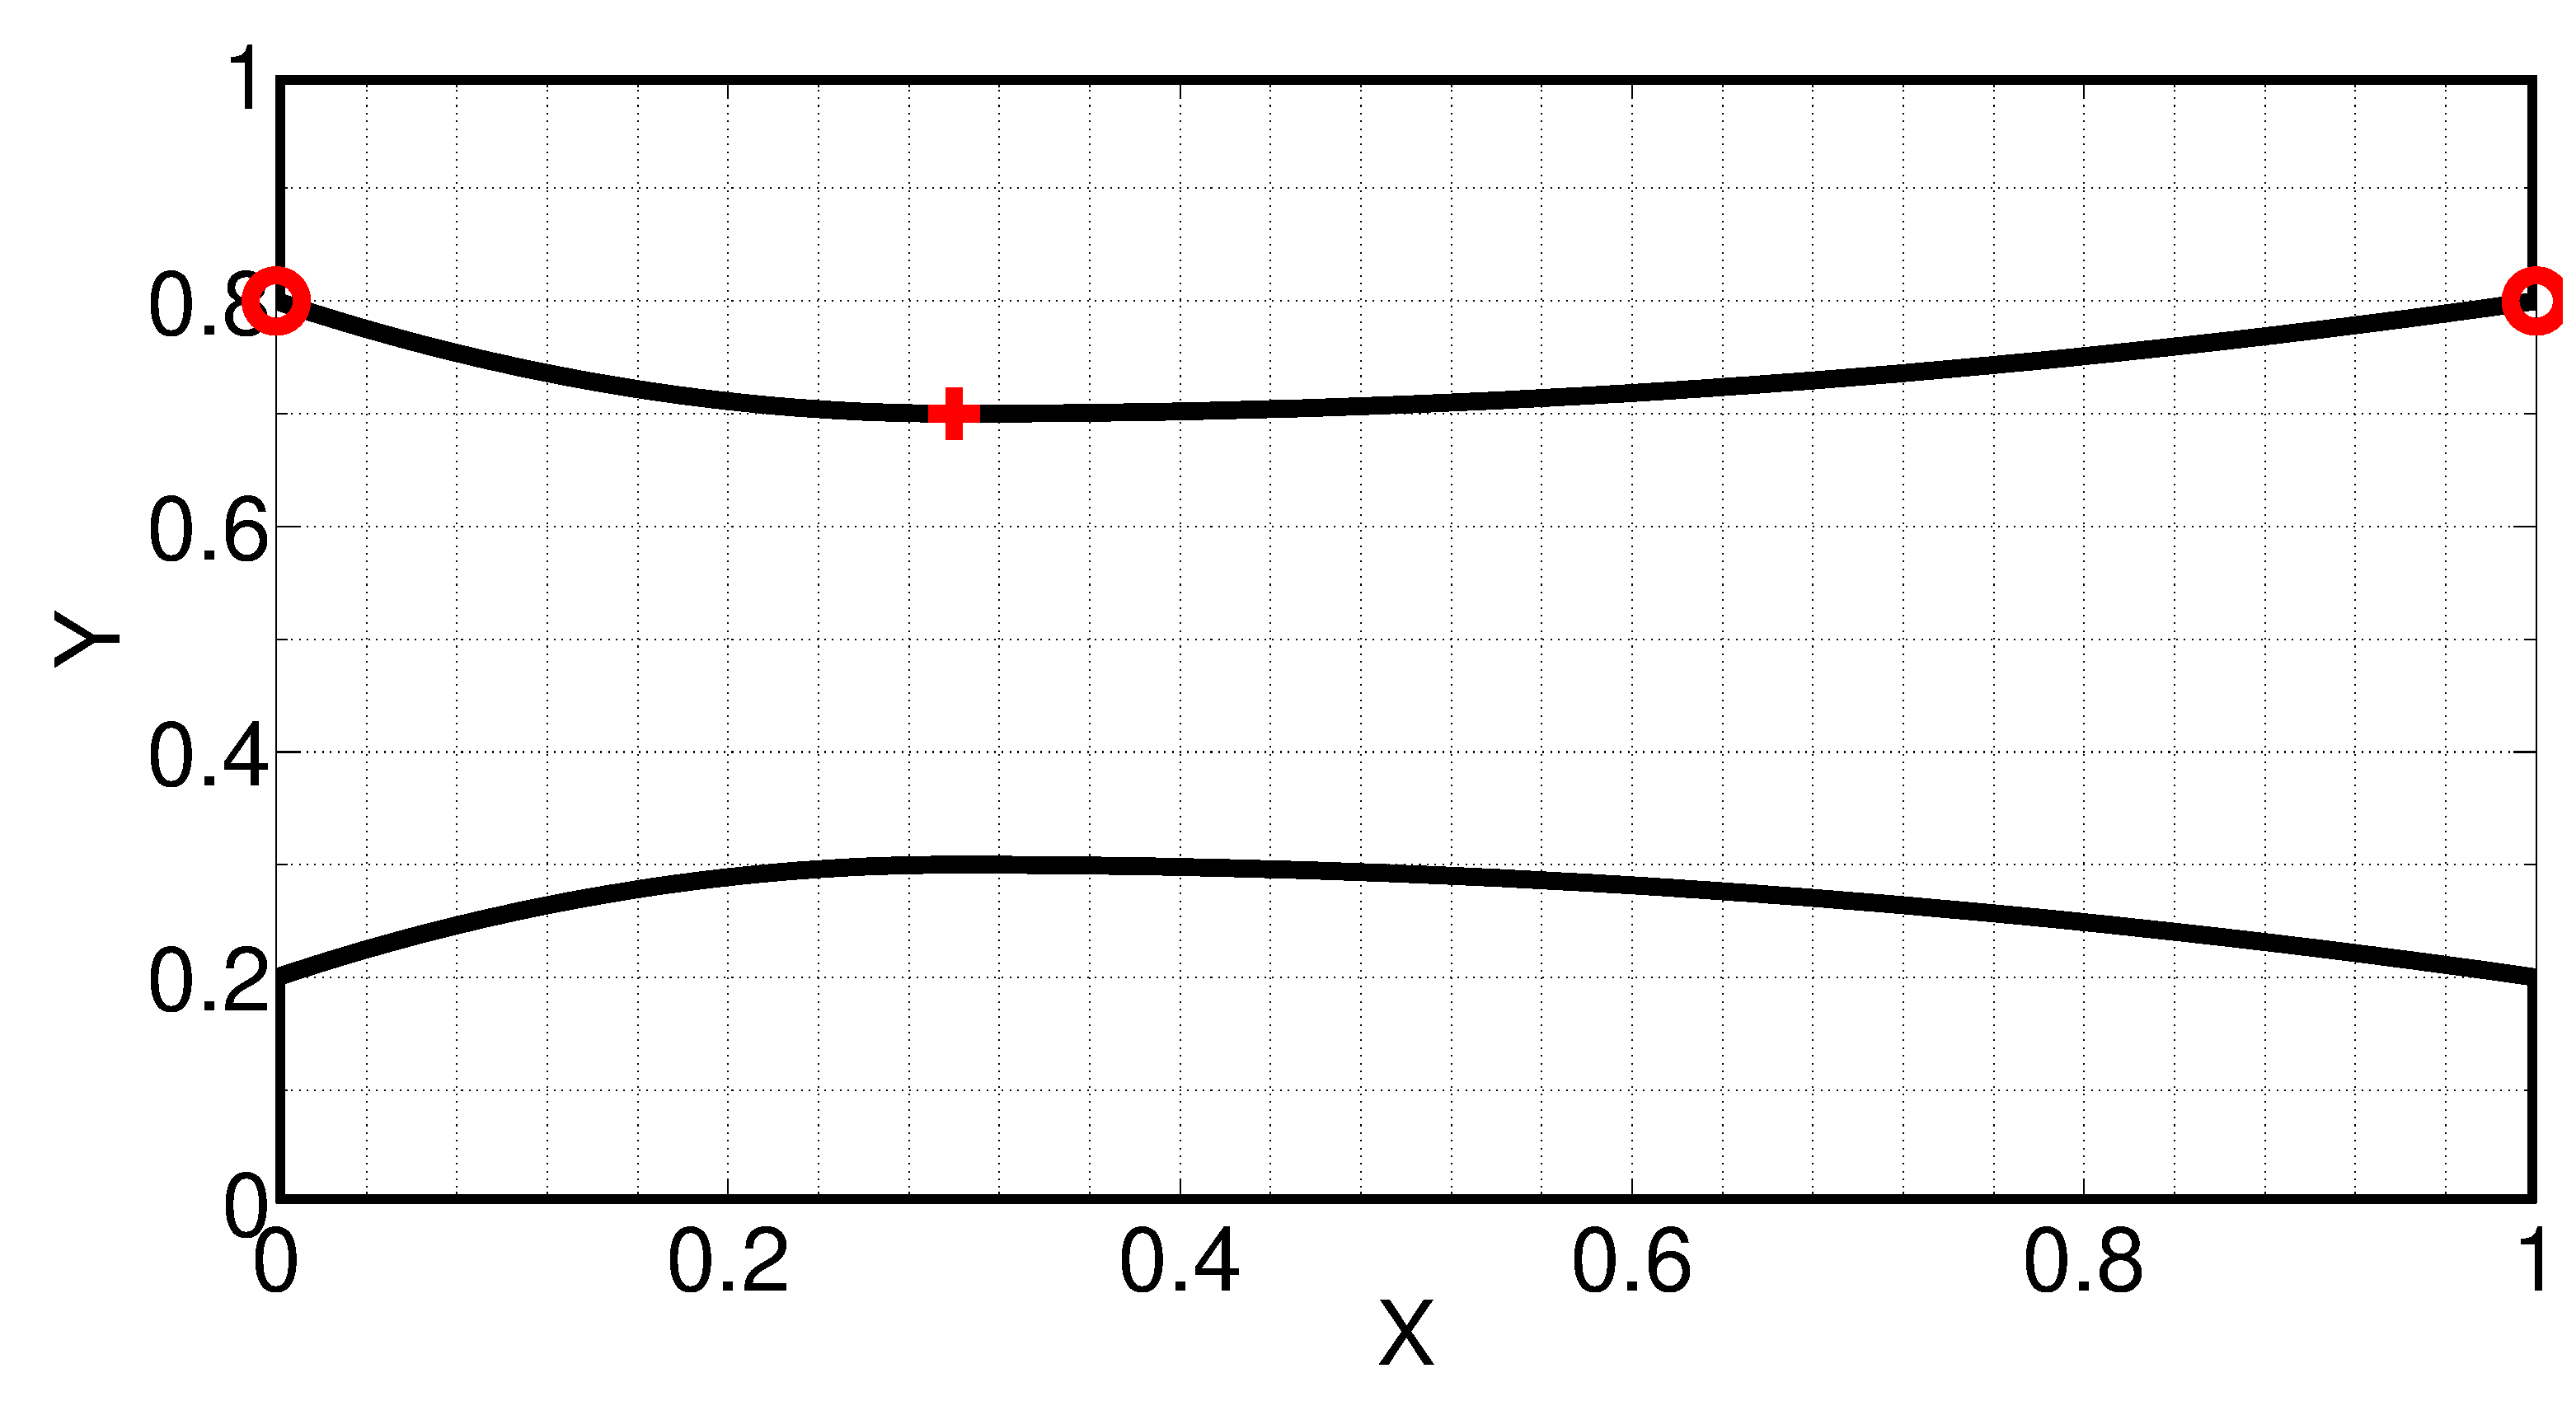
\includegraphics[width=6.5cm]{Chapter_4/figure/flow_through_nozzle/nozzle_shape_yt02.eps}
    }
    \caption{Effect of design variable on the shape of the nozzle.}
    \label{fig:C4_nozzleShape}
\end{figure}
%
The mesh convergence plots for the governing equations are shown in Figure \ref{fig:C4_nozzleFlow_meshConvergence}. As shown here, the mesh size of $500 \times 125$ is selected for the analysis.
%
\begin{figure}[H]
    \centering
    \subfigure[U-velocity mesh convergence.]
    {
    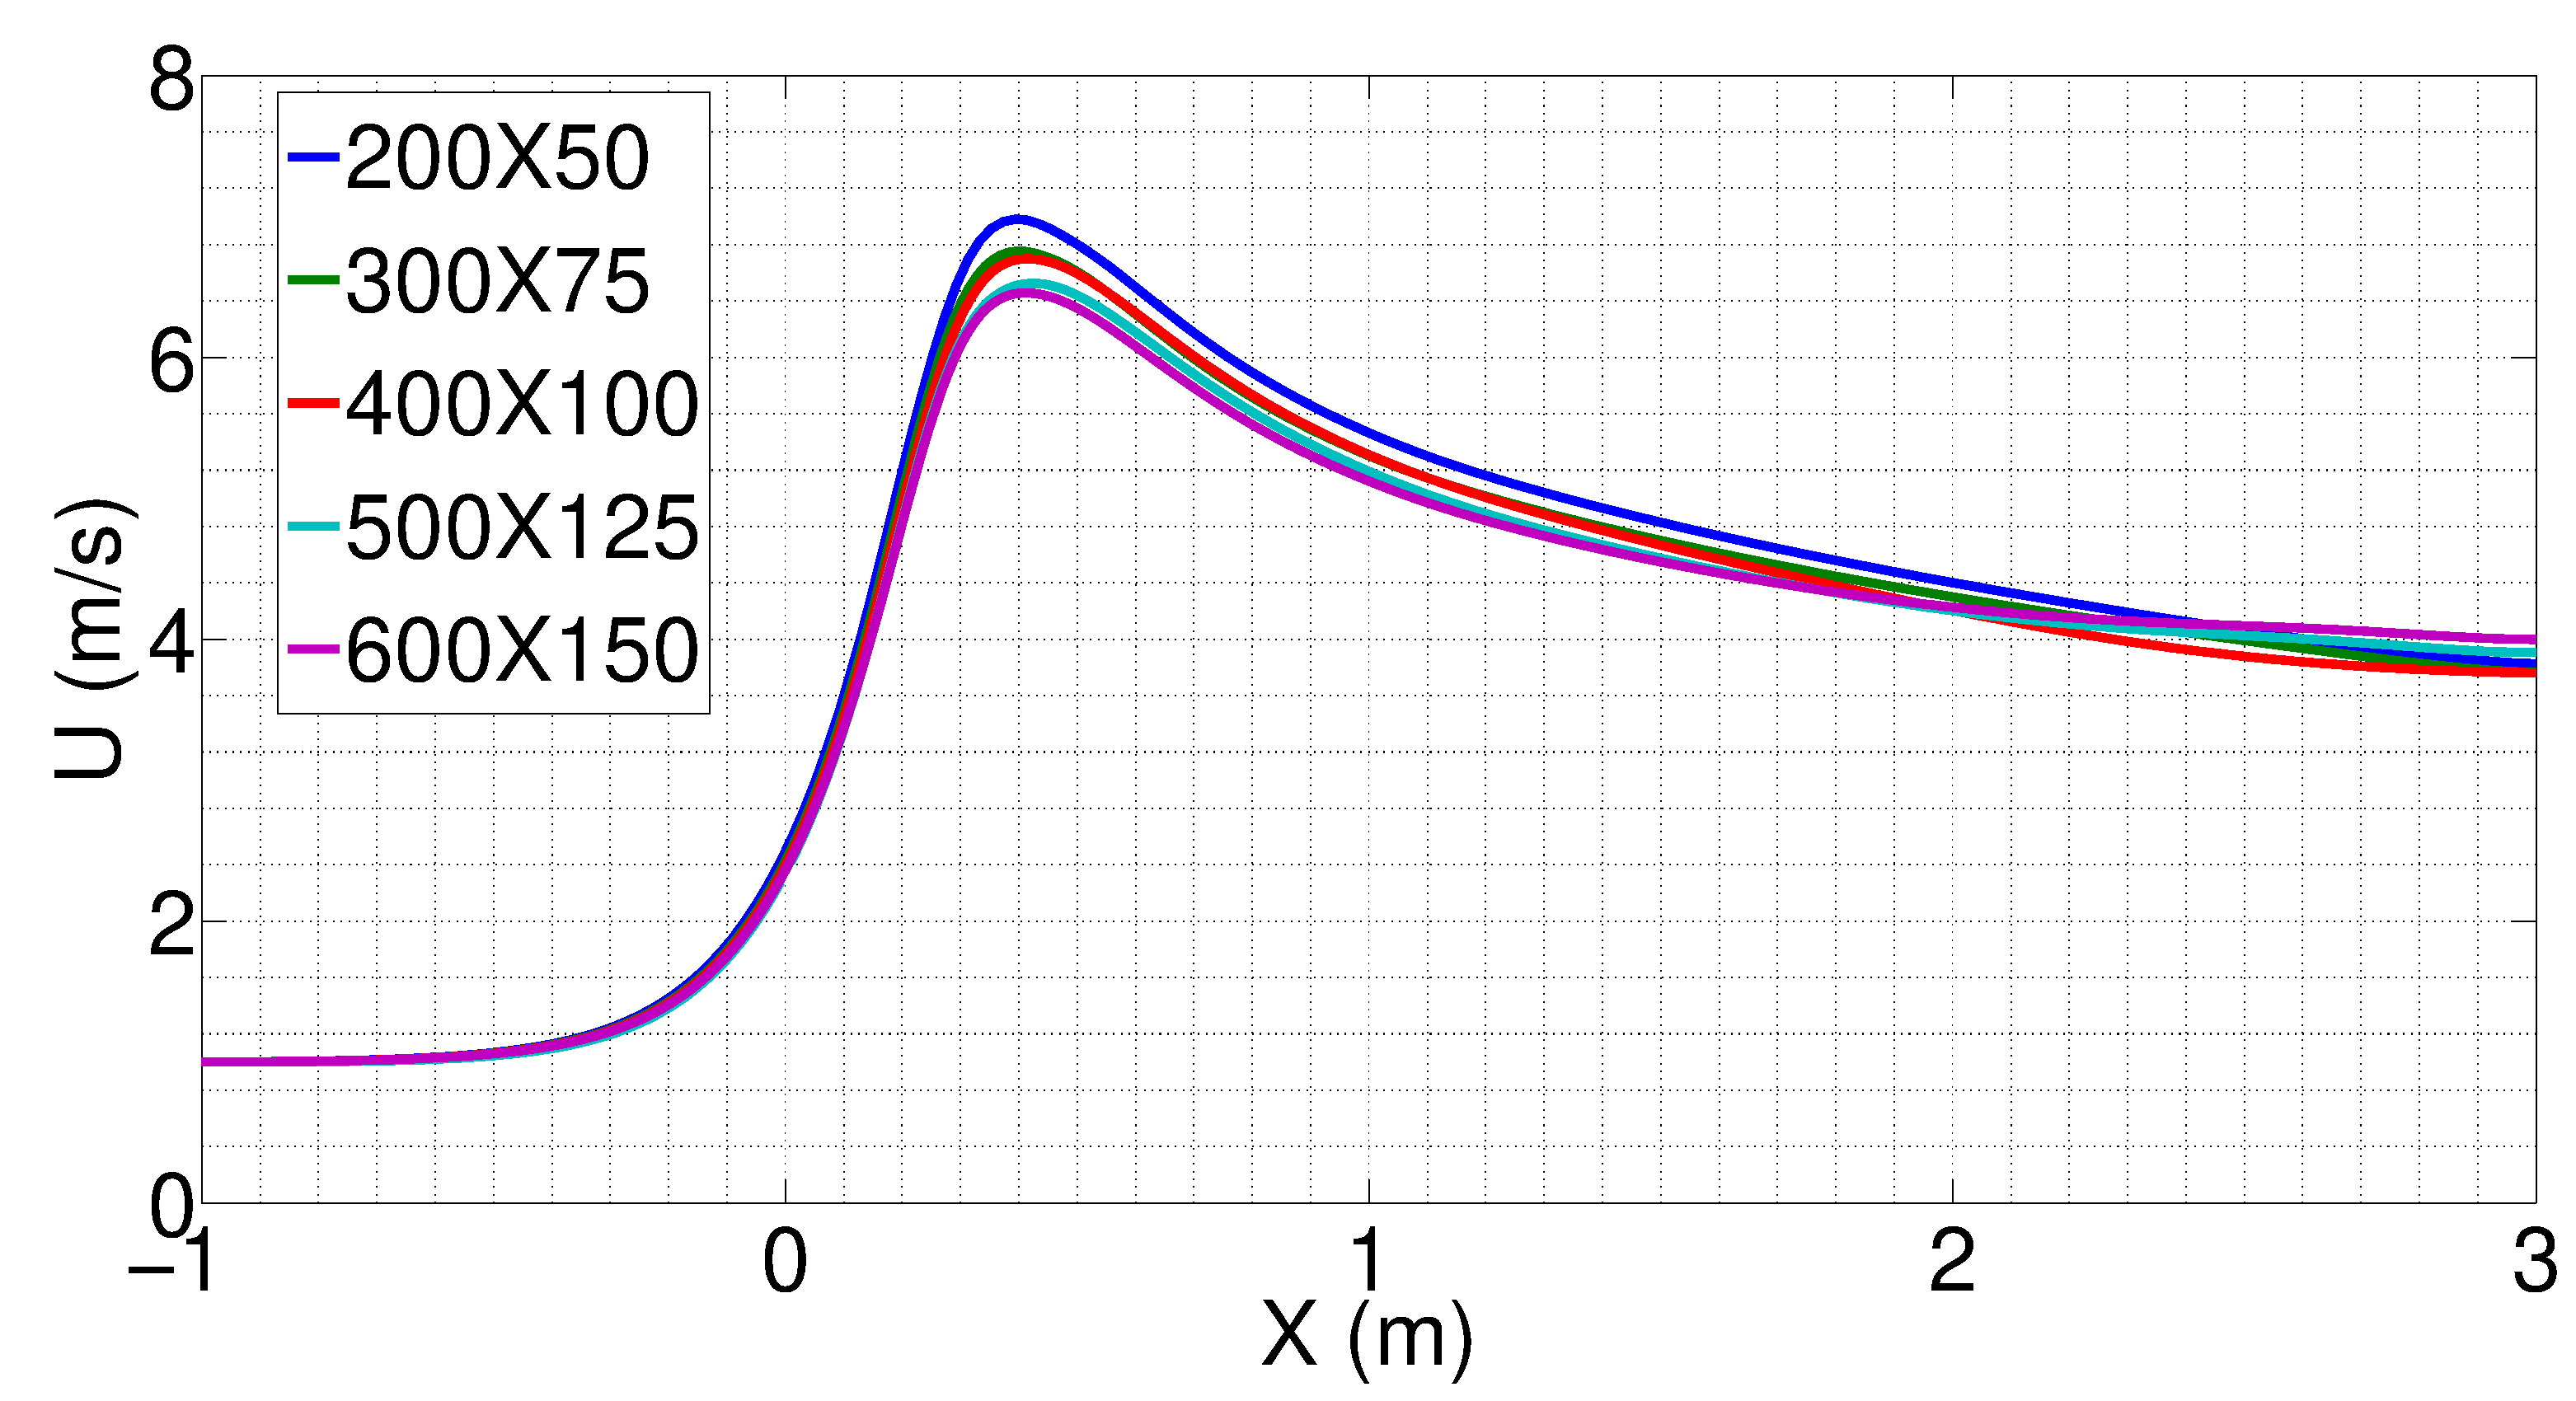
\includegraphics[width=6.5cm]{Chapter_4/figure/flow_through_nozzle/convergence_U_RE100.eps}
    }
    \quad
    \subfigure[V-velocity mesh convergence.]
    {
    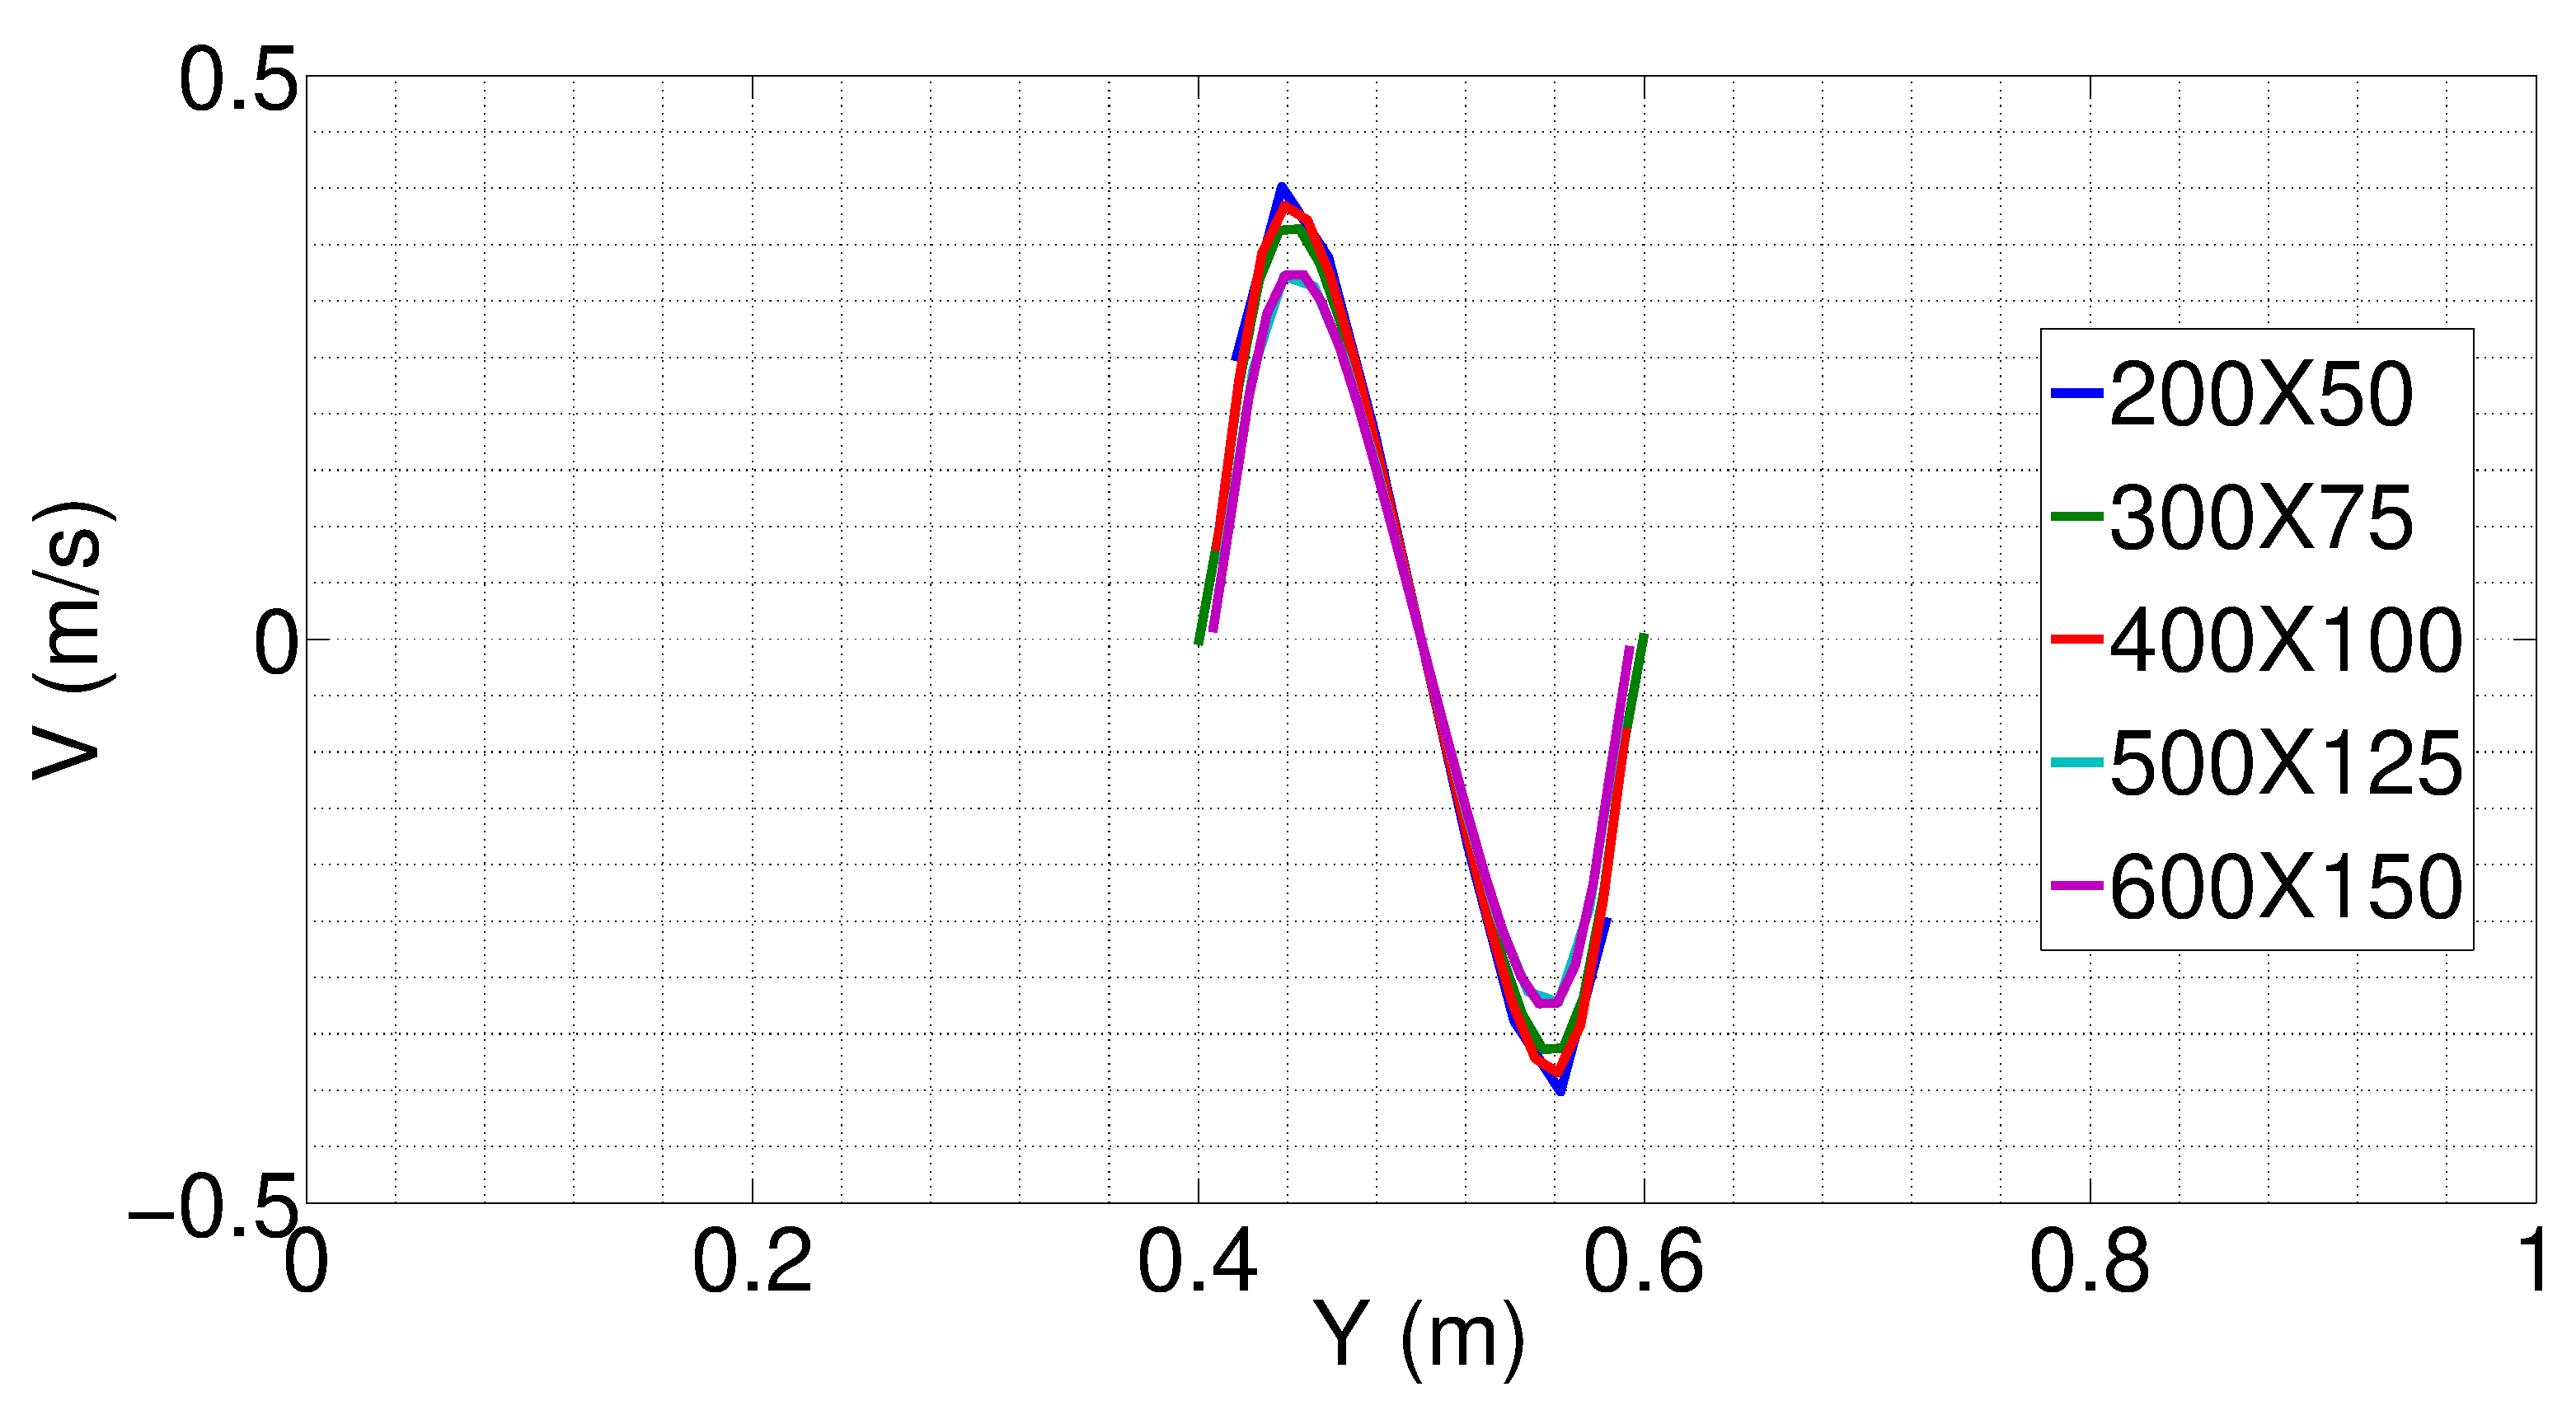
\includegraphics[width=6.5cm]{Chapter_4/figure/flow_through_nozzle/convergence_V_RE100.eps}
    }
    \\
    \subfigure[Pressure mesh convergence.]
    {
    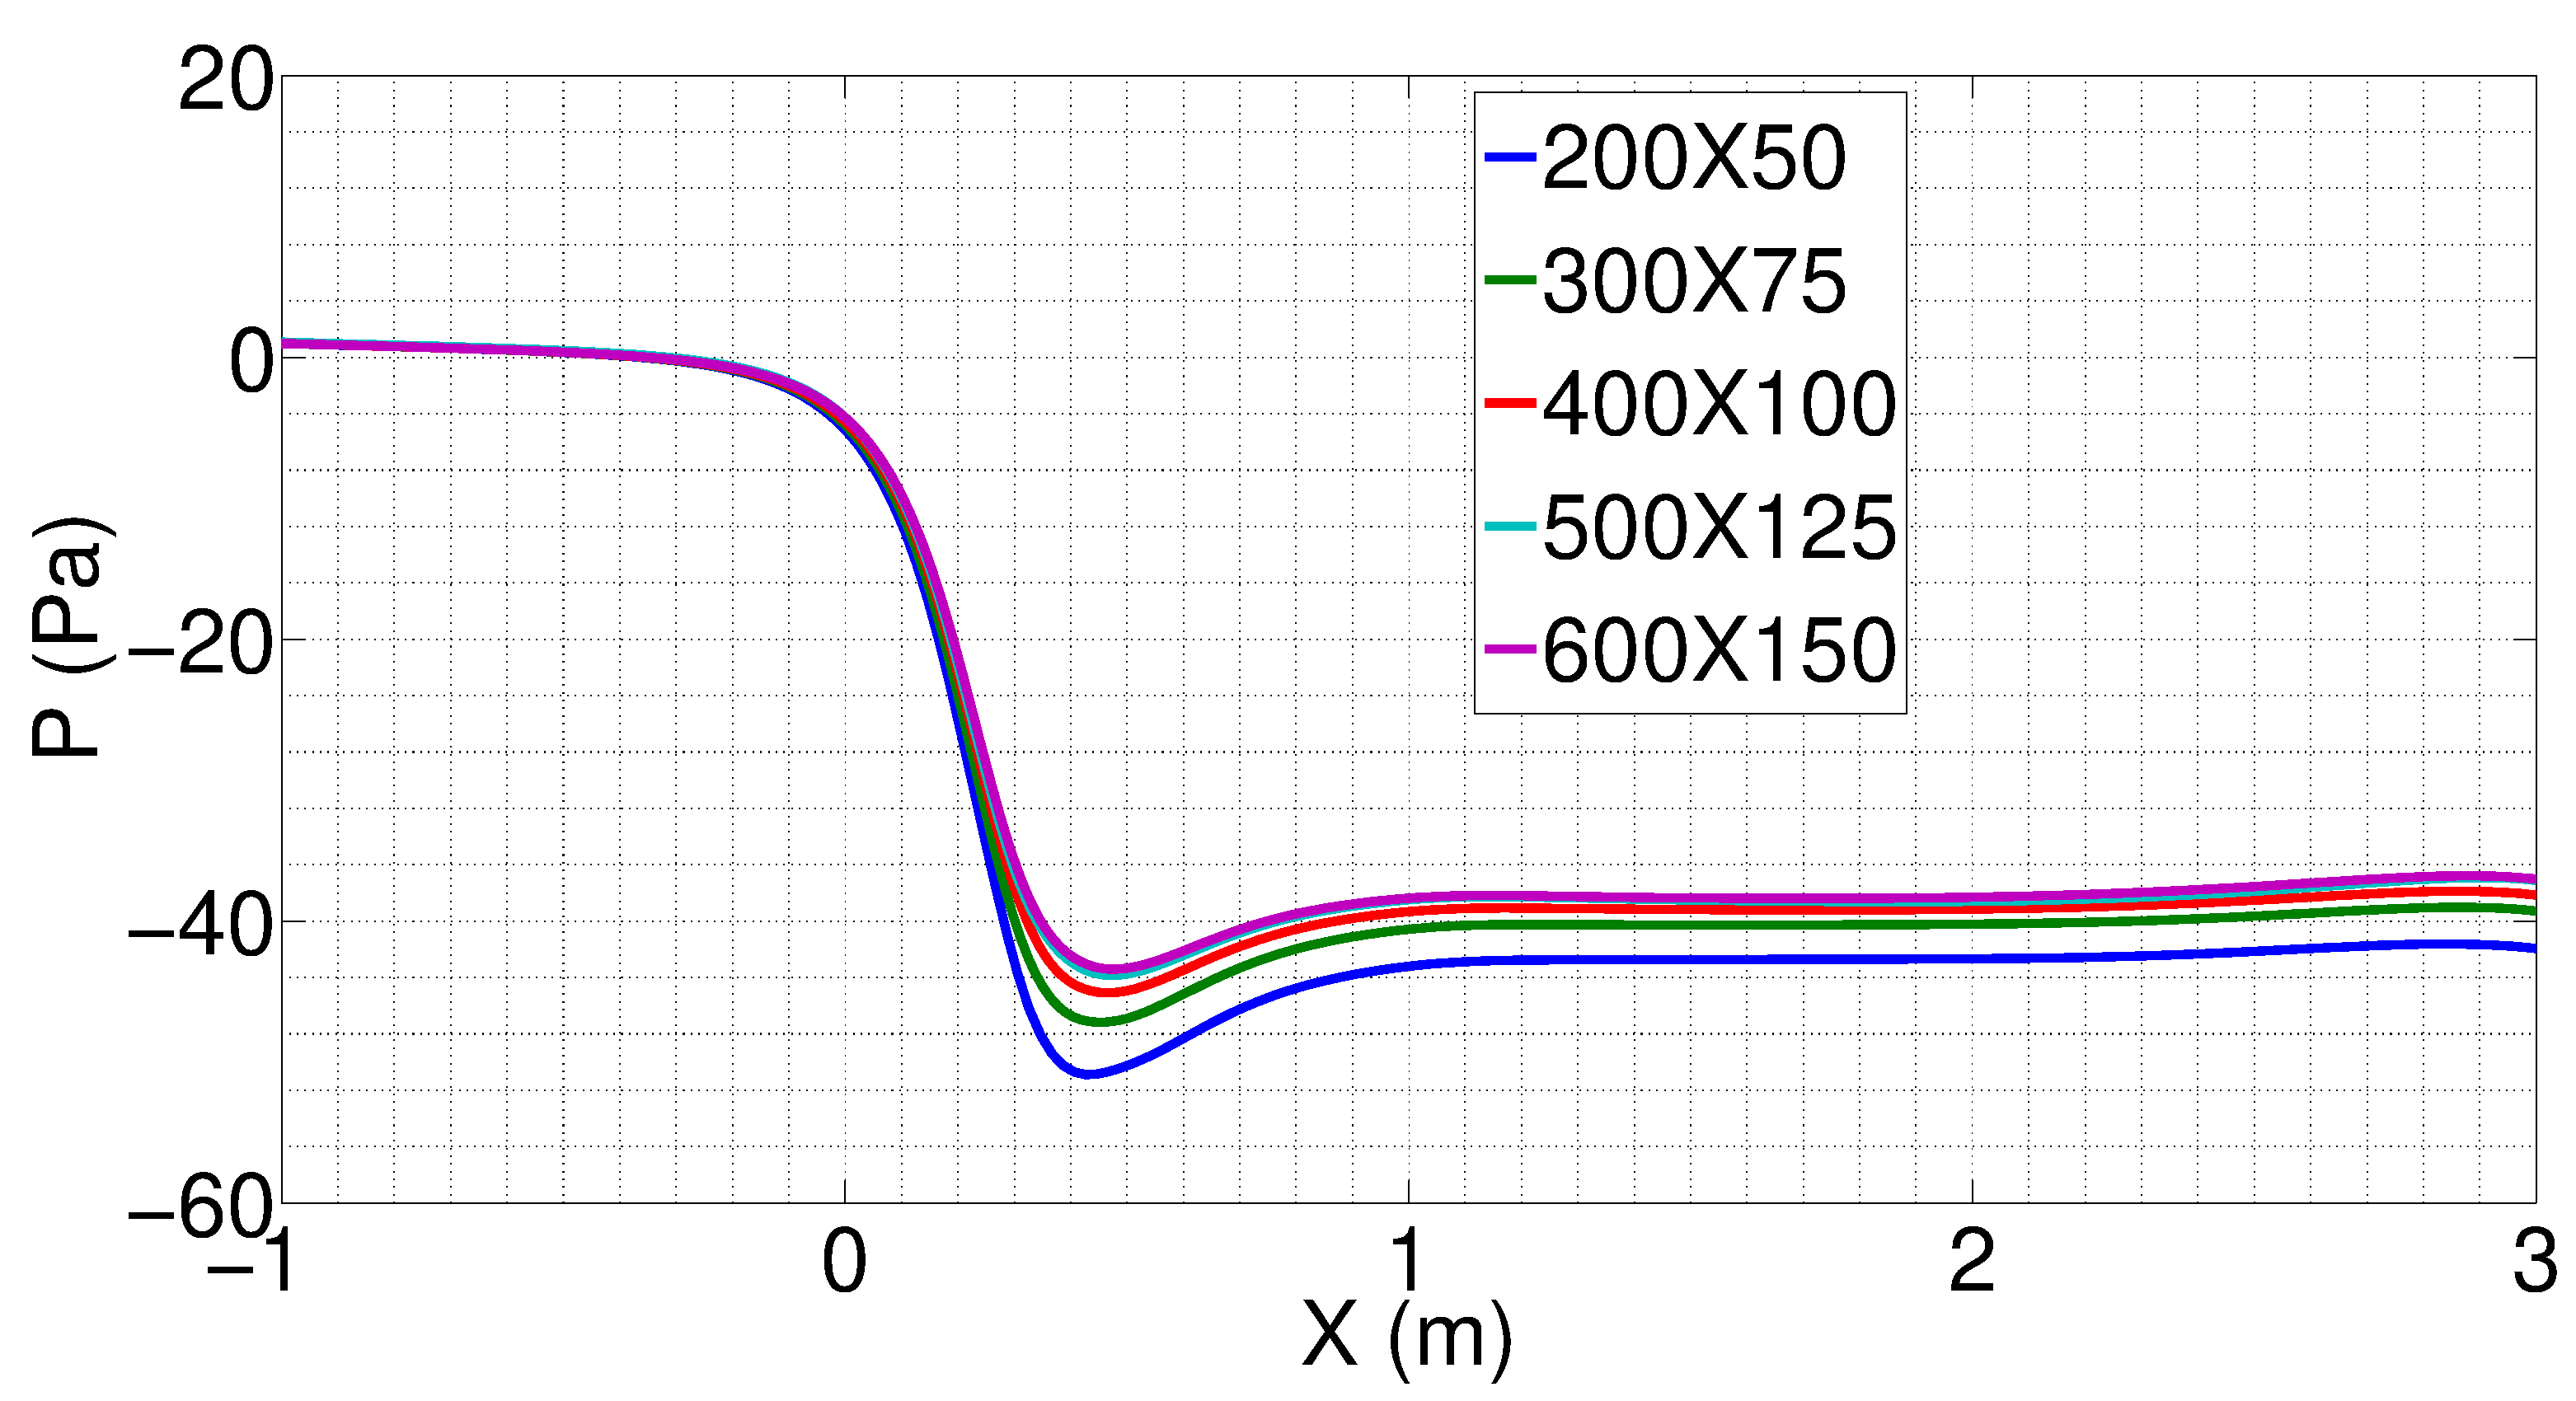
\includegraphics[width=6.5cm]{Chapter_4/figure/flow_through_nozzle/convergence_P_RE100.eps}
    }
    \caption{Mesh convergence study for the governing equation. The dashed line represent the fitted curve through points.}
    \label{fig:C4_nozzleFlow_meshConvergence}
\end{figure}
%
The convergence rate is shown in Figure \ref{fig:C4_nozzleFlow_meshConvergenceRate}. A mesh node at the throat area on the symmetry line is selected for this study for u-velocity and pressure. Since the v-velocity is zero for this point, a node at $(0.3, 0
.55)$ is selected for the convergence study of the v-velocity. The slope of the dotted line in Figure \ref{fig:C4_nozzleFlow_meshConvergenceRate} is calculated as $-0.96$, $-0.86$, and $-0.73$ for u-velocity, v-velocity, and pressure error, respectfully. The convergence is close to first order due to the relative location of the points to the solid walls where the approximation is first order.
%
\begin{figure}[H]
    \centering
    \subfigure[U-velocity convergence rate at $(0.3, 0.0)$.]
    {
    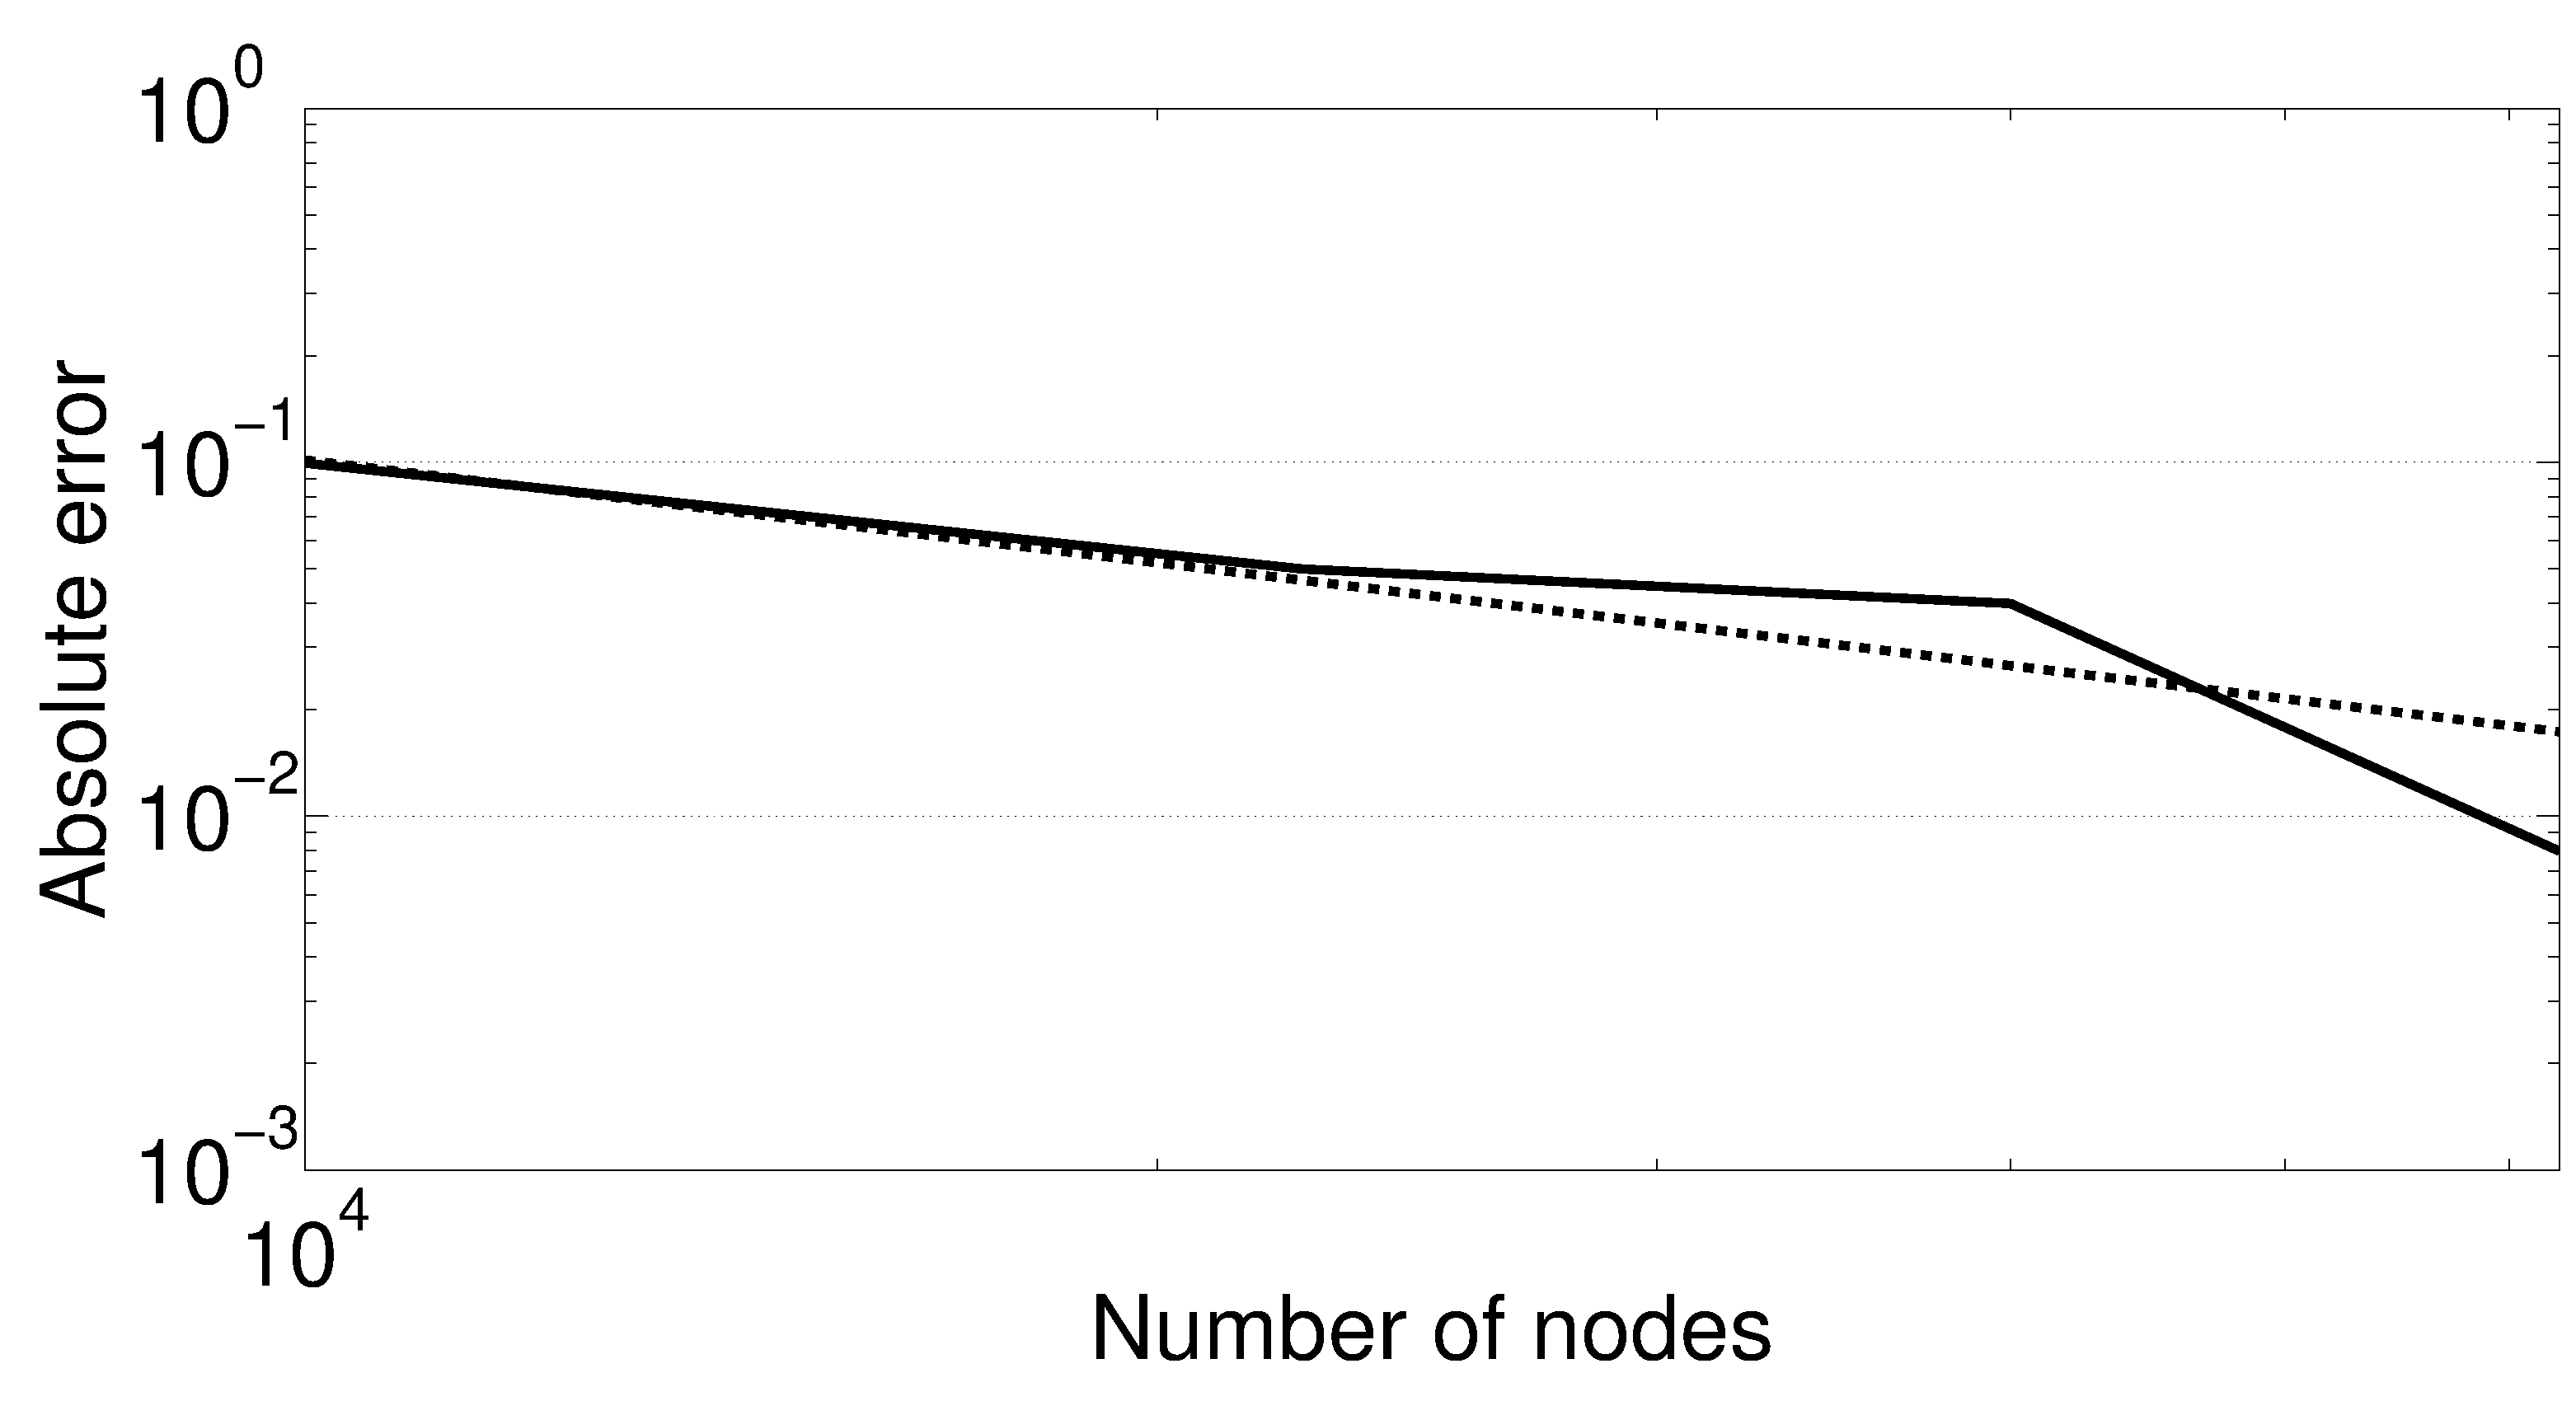
\includegraphics[width=6.5cm]{Chapter_4/figure/flow_through_nozzle/convergenceRate_U_RE100.eps}
    }
    \quad
    \subfigure[V-velocity convergence rate at $(0.3, 0.55)$.]
    {
    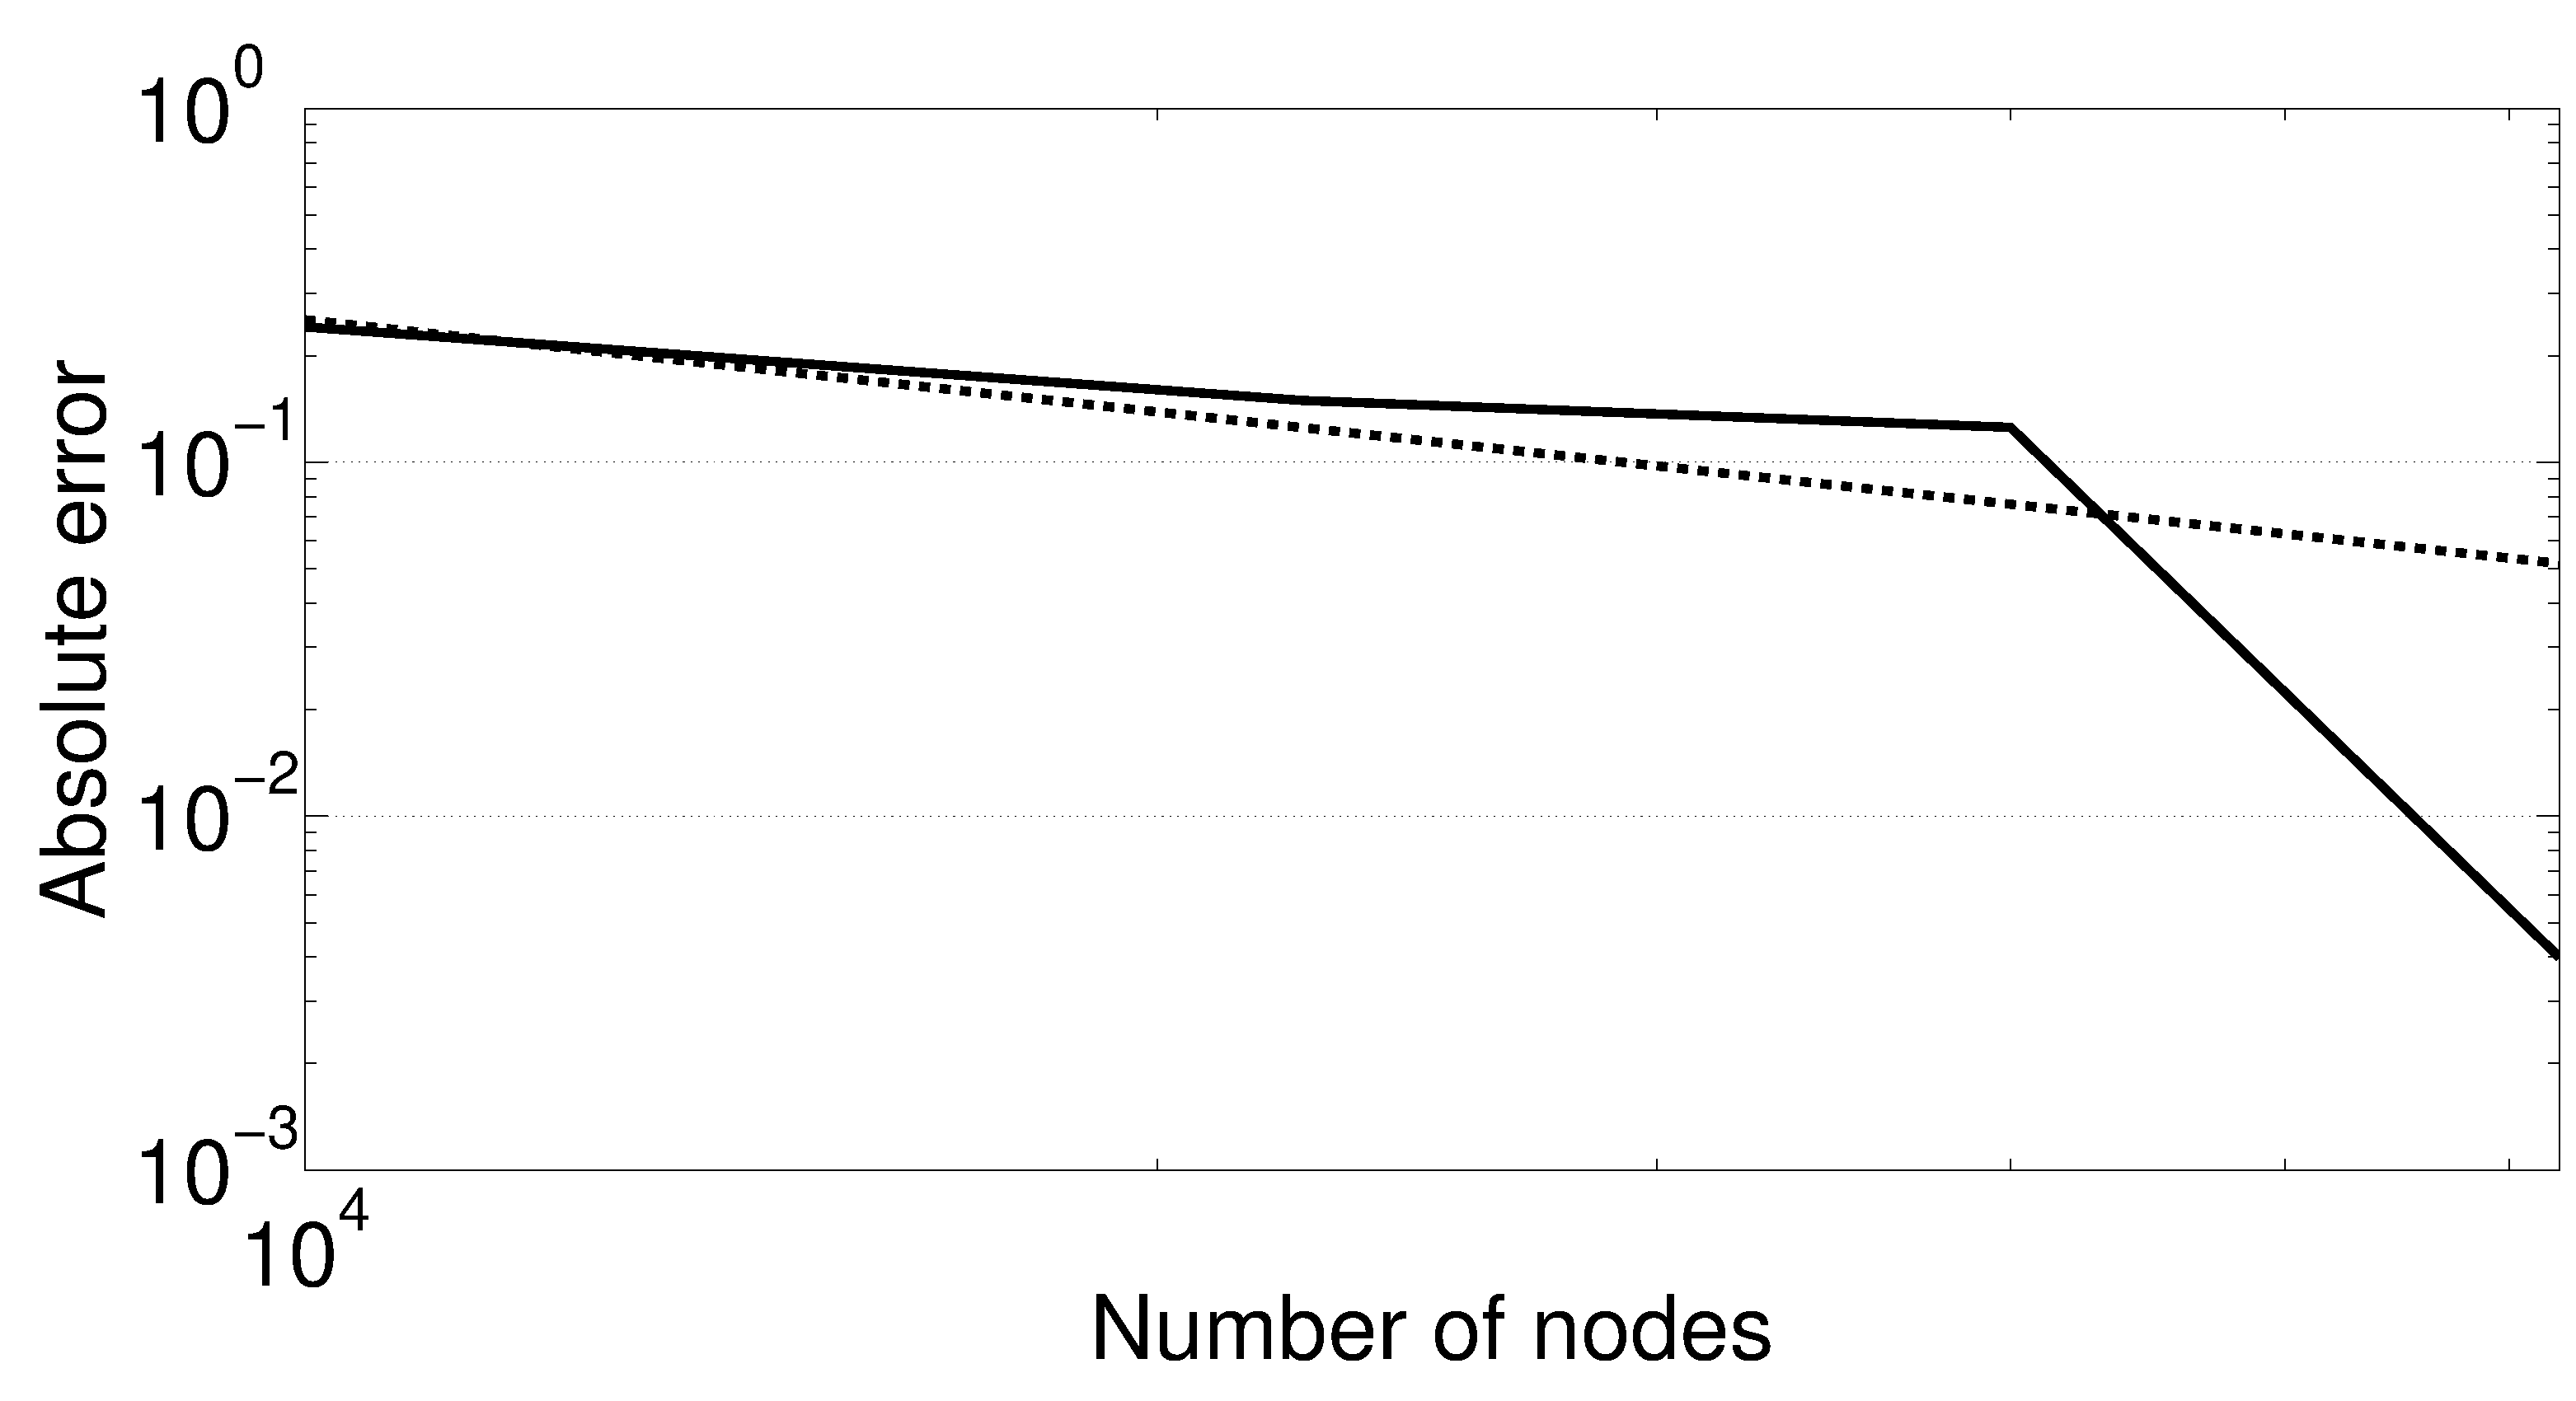
\includegraphics[width=6.5cm]{Chapter_4/figure/flow_through_nozzle/convergenceRate_V_RE100.eps}
    }
    \\
    \subfigure[Pressure  convergence rate at $(0.3, 0.0)$..]
    {
    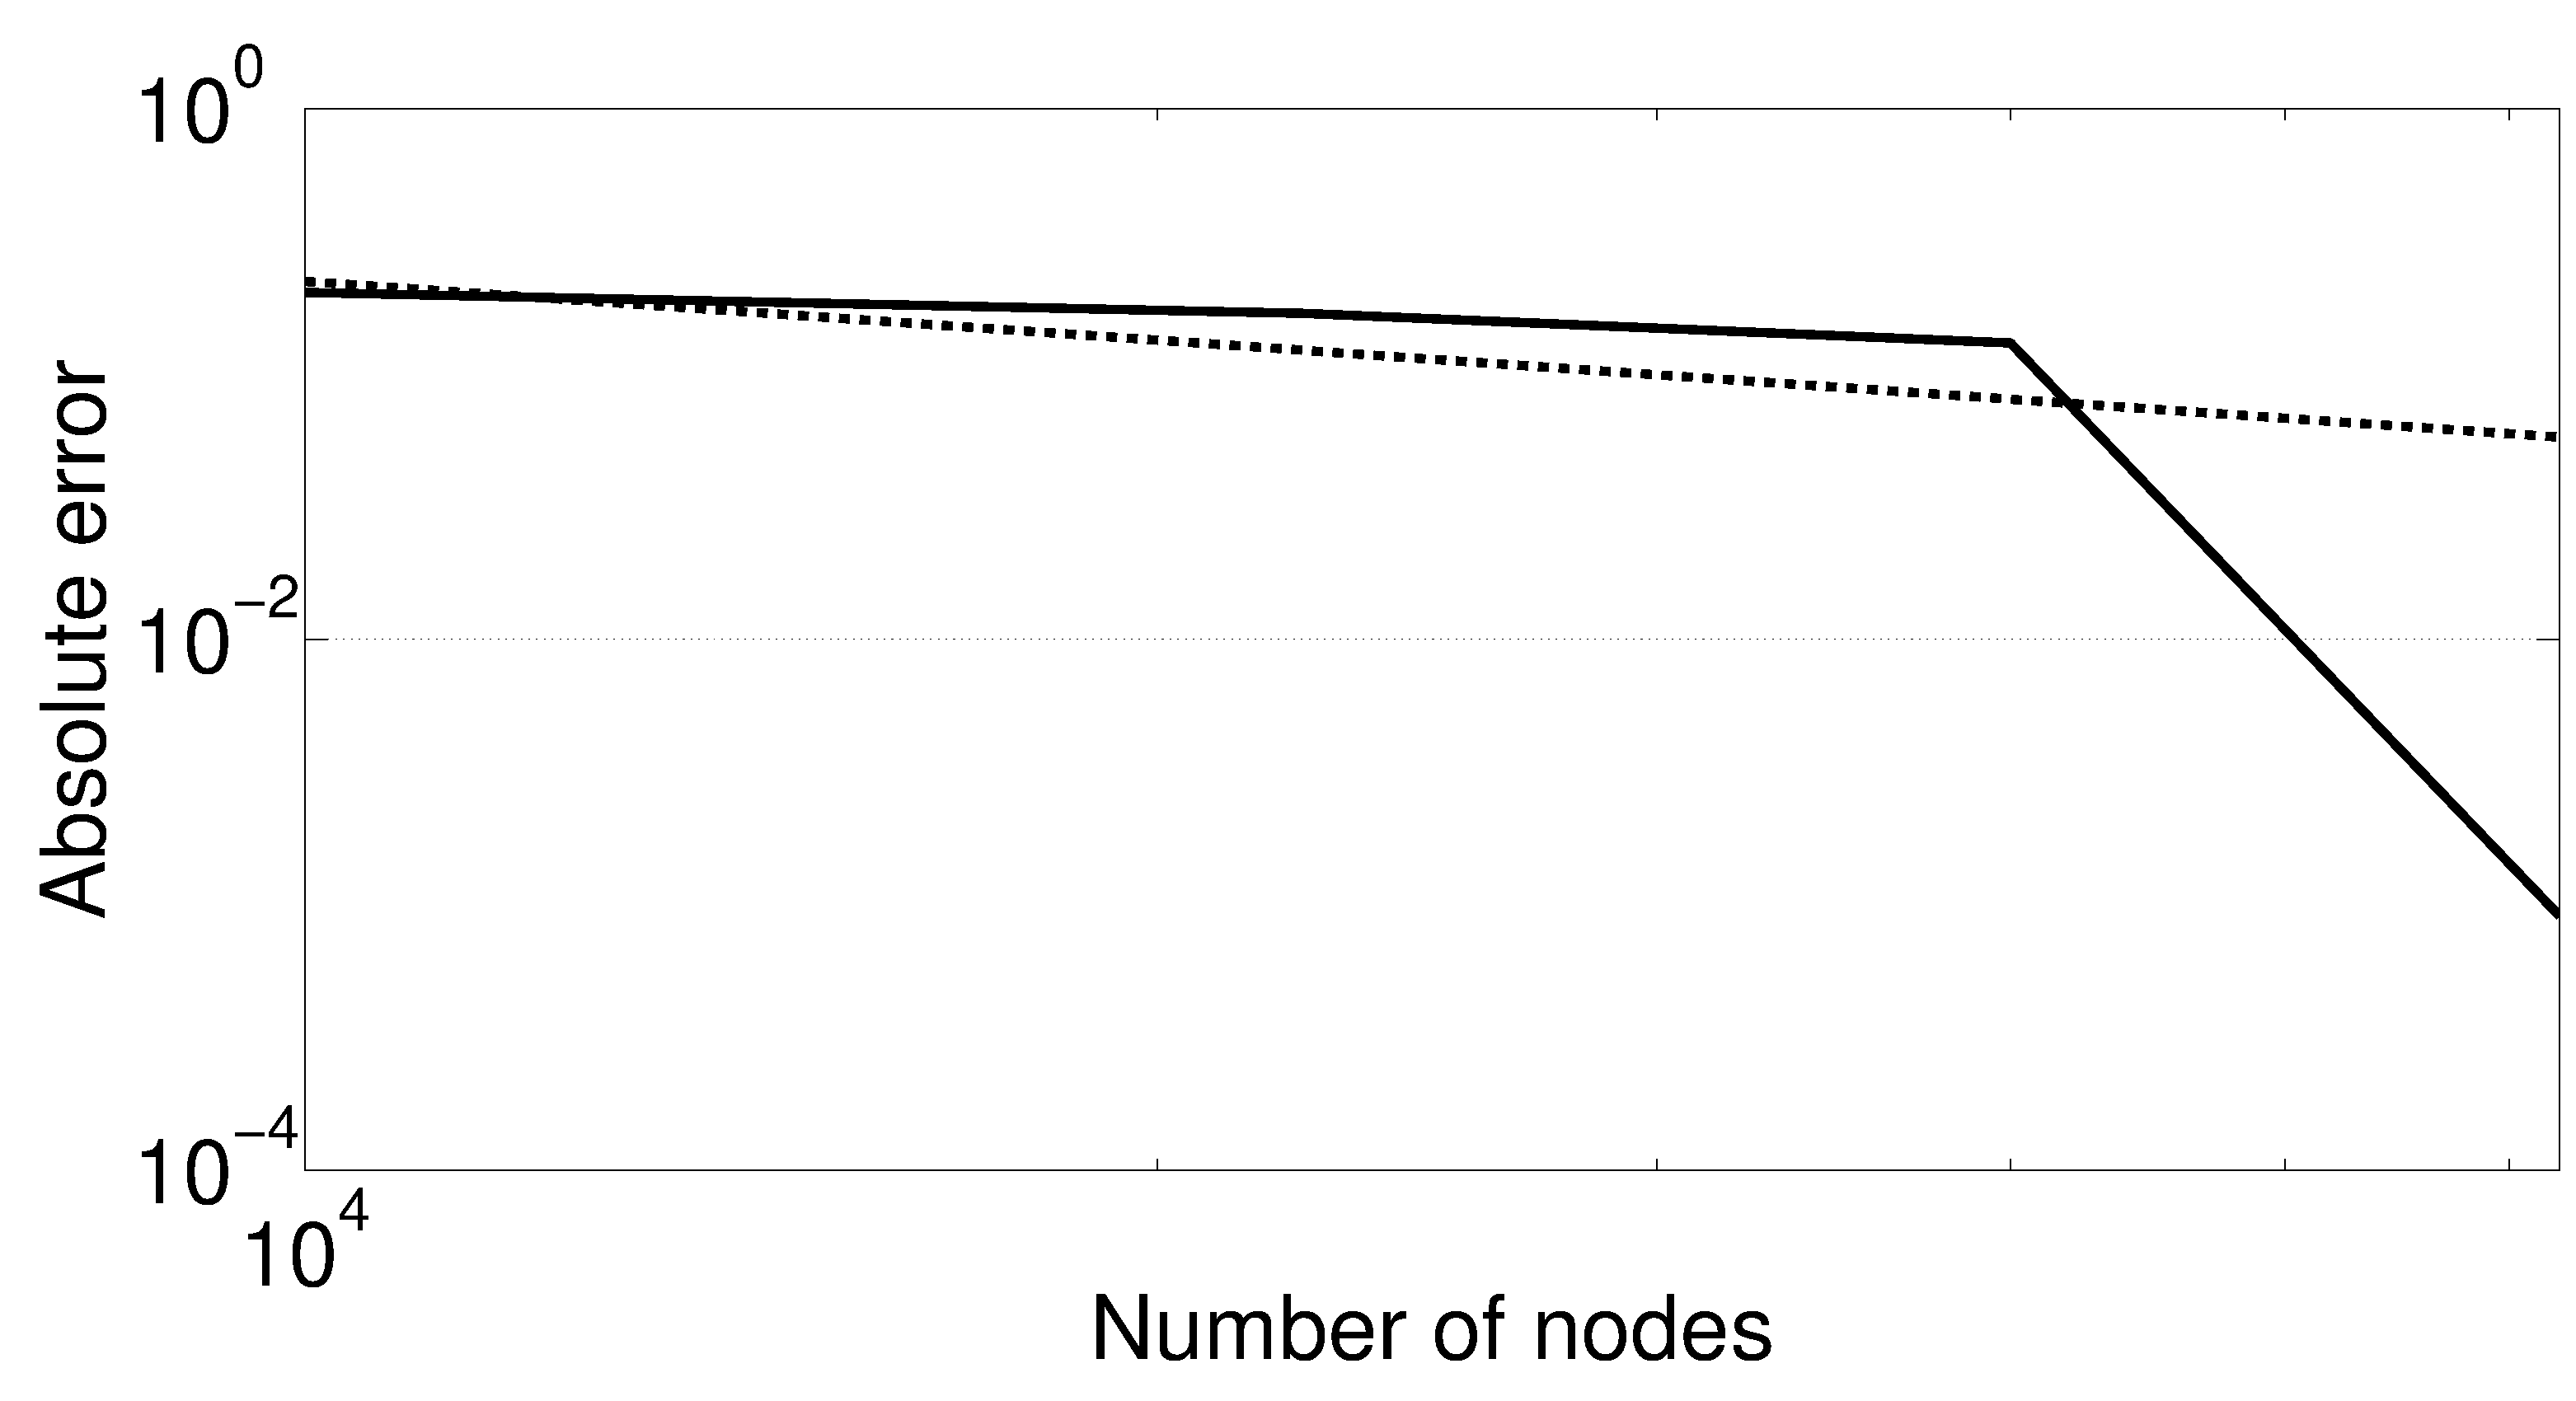
\includegraphics[width=6.5cm]{Chapter_4/figure/flow_through_nozzle/convergenceRate_P_RE100.eps}
    }
    \caption{Mesh convergence study for the governing equation.}
    \label{fig:C4_nozzleFlow_meshConvergenceRate}
\end{figure}
%
The contour plots for the velocities through the nozzle are shown in Figure \ref{fig:C4_nozzleFlow_contourForAnalysis}. As shown here, the forcing function was able to model the walls and cause the flow to accelerate through the nozzle.
%
\begin{figure}[H]
    \centering
    \subfigure[U-velocity contour.]
    {
    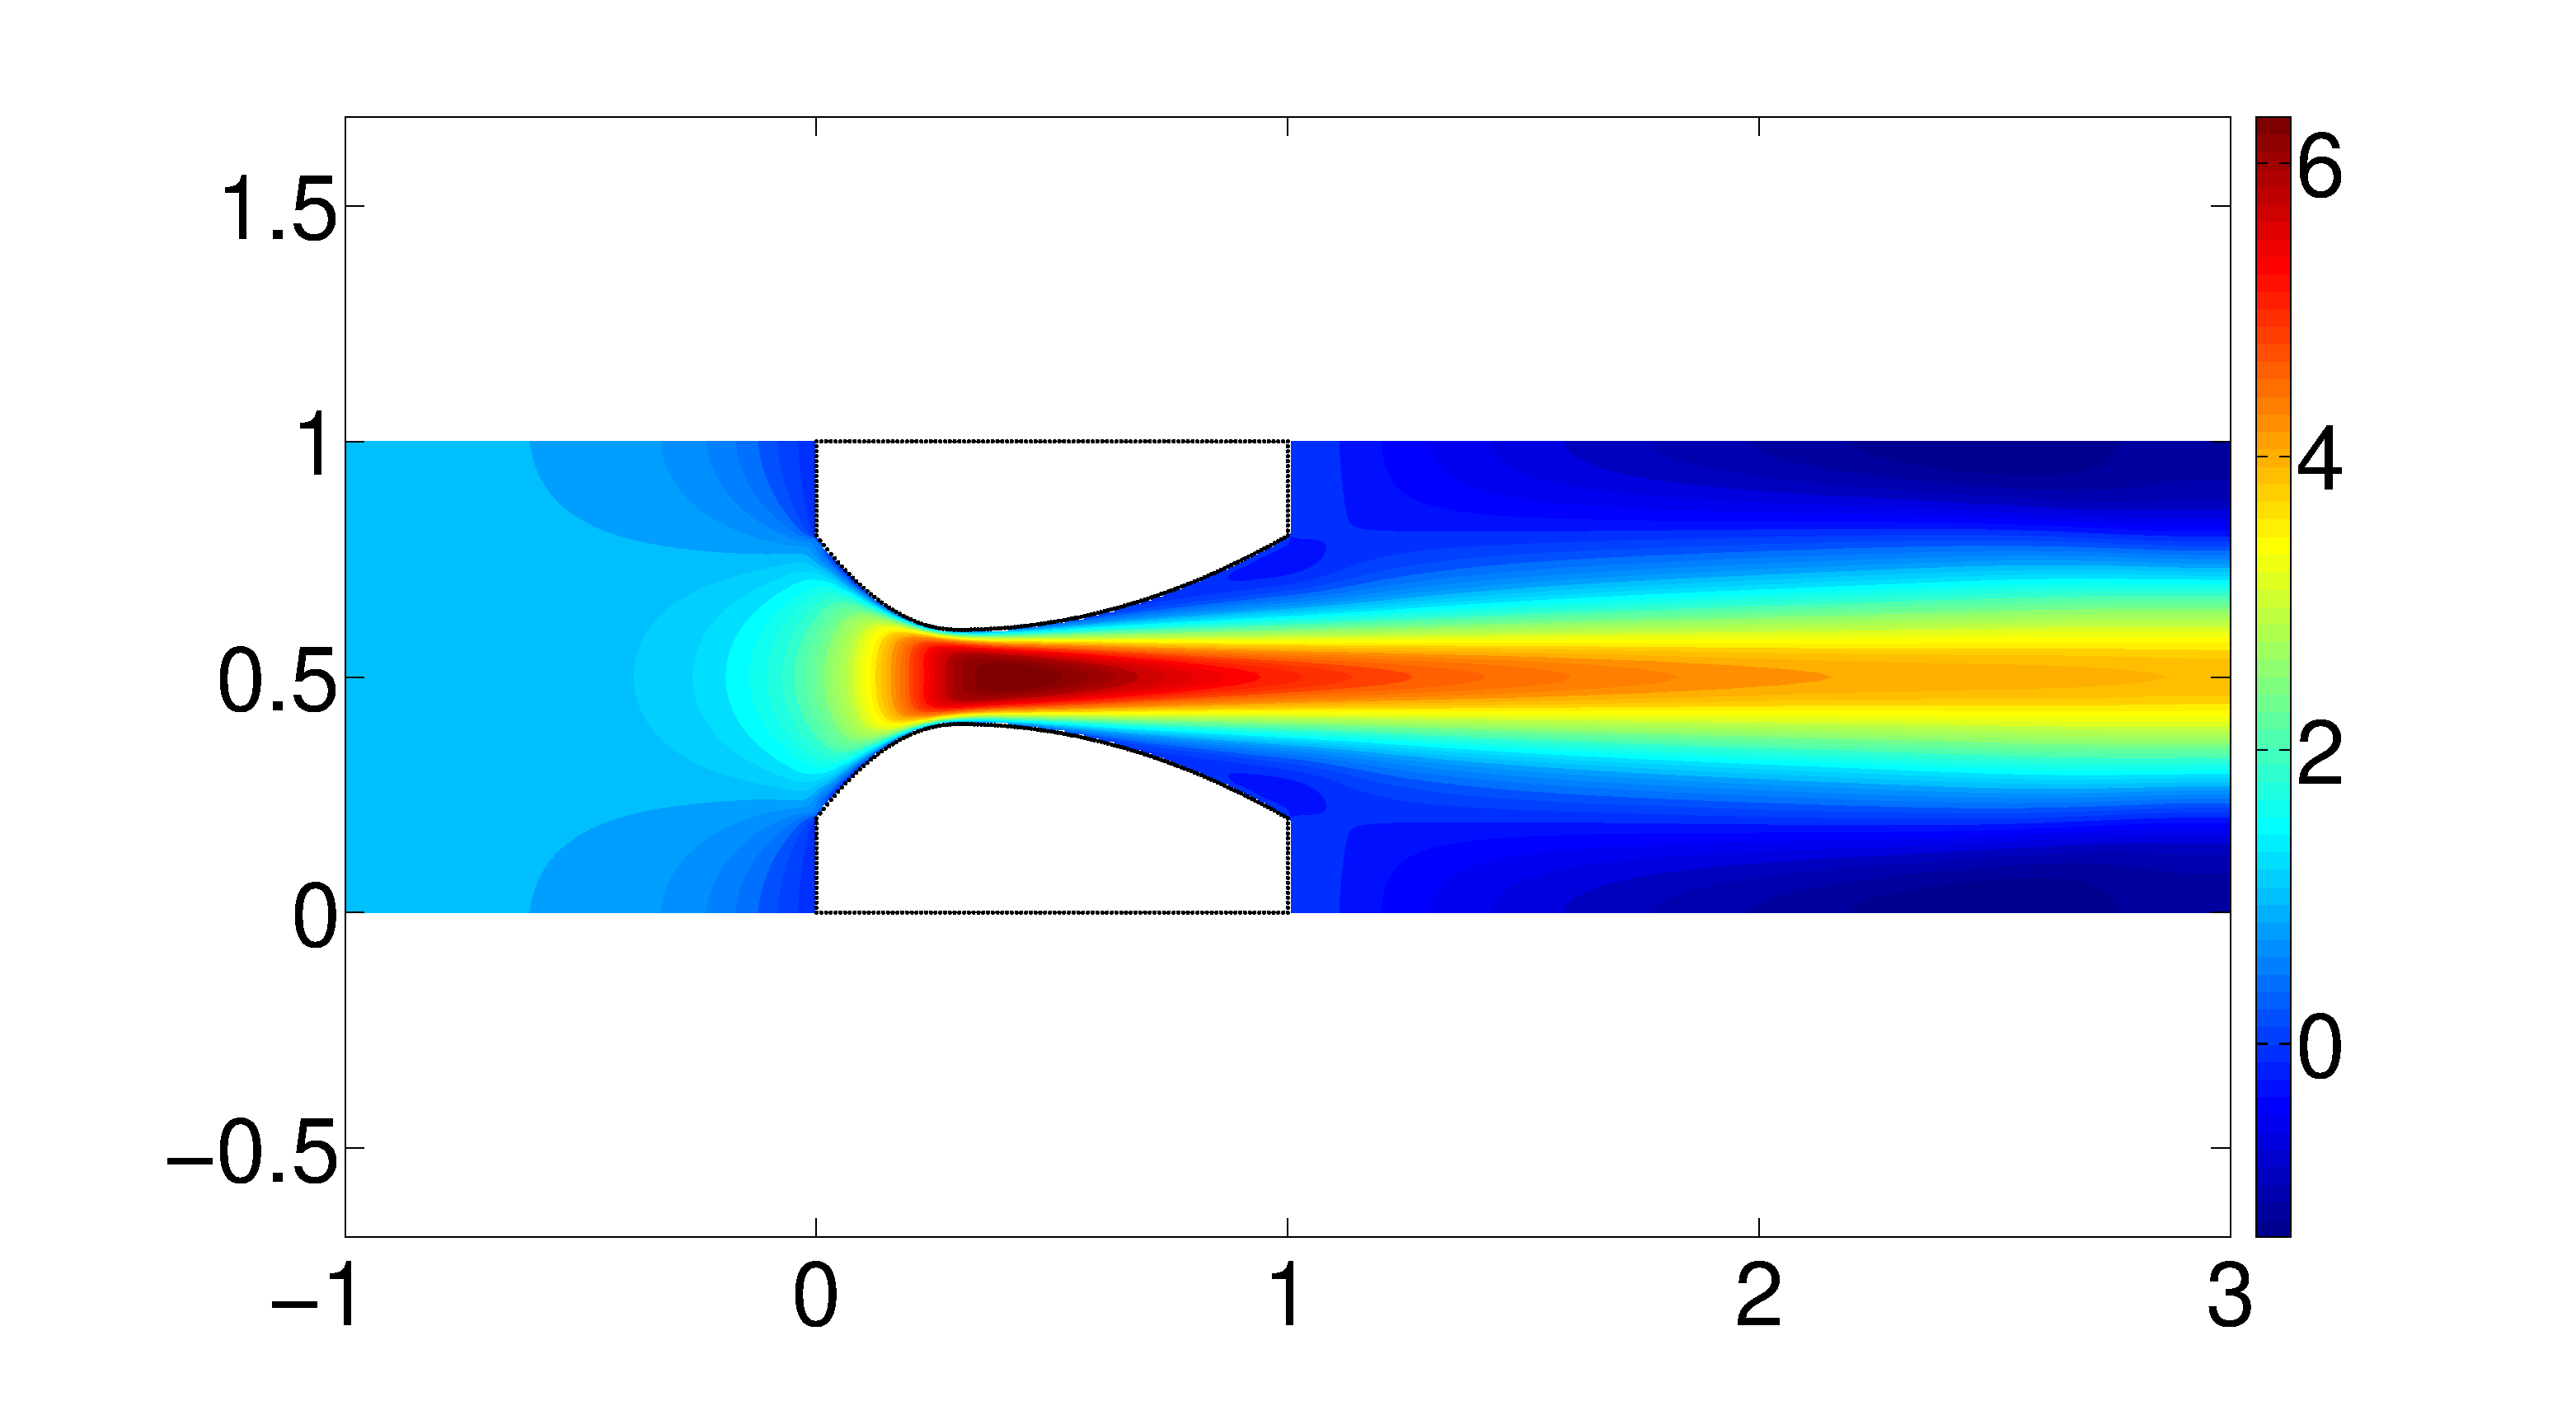
\includegraphics[width=6.5cm]{Chapter_4/figure/flow_through_nozzle/contour_U_RE100.eps}
    }
    \quad
    \subfigure[V-velocity contour.]
    {
    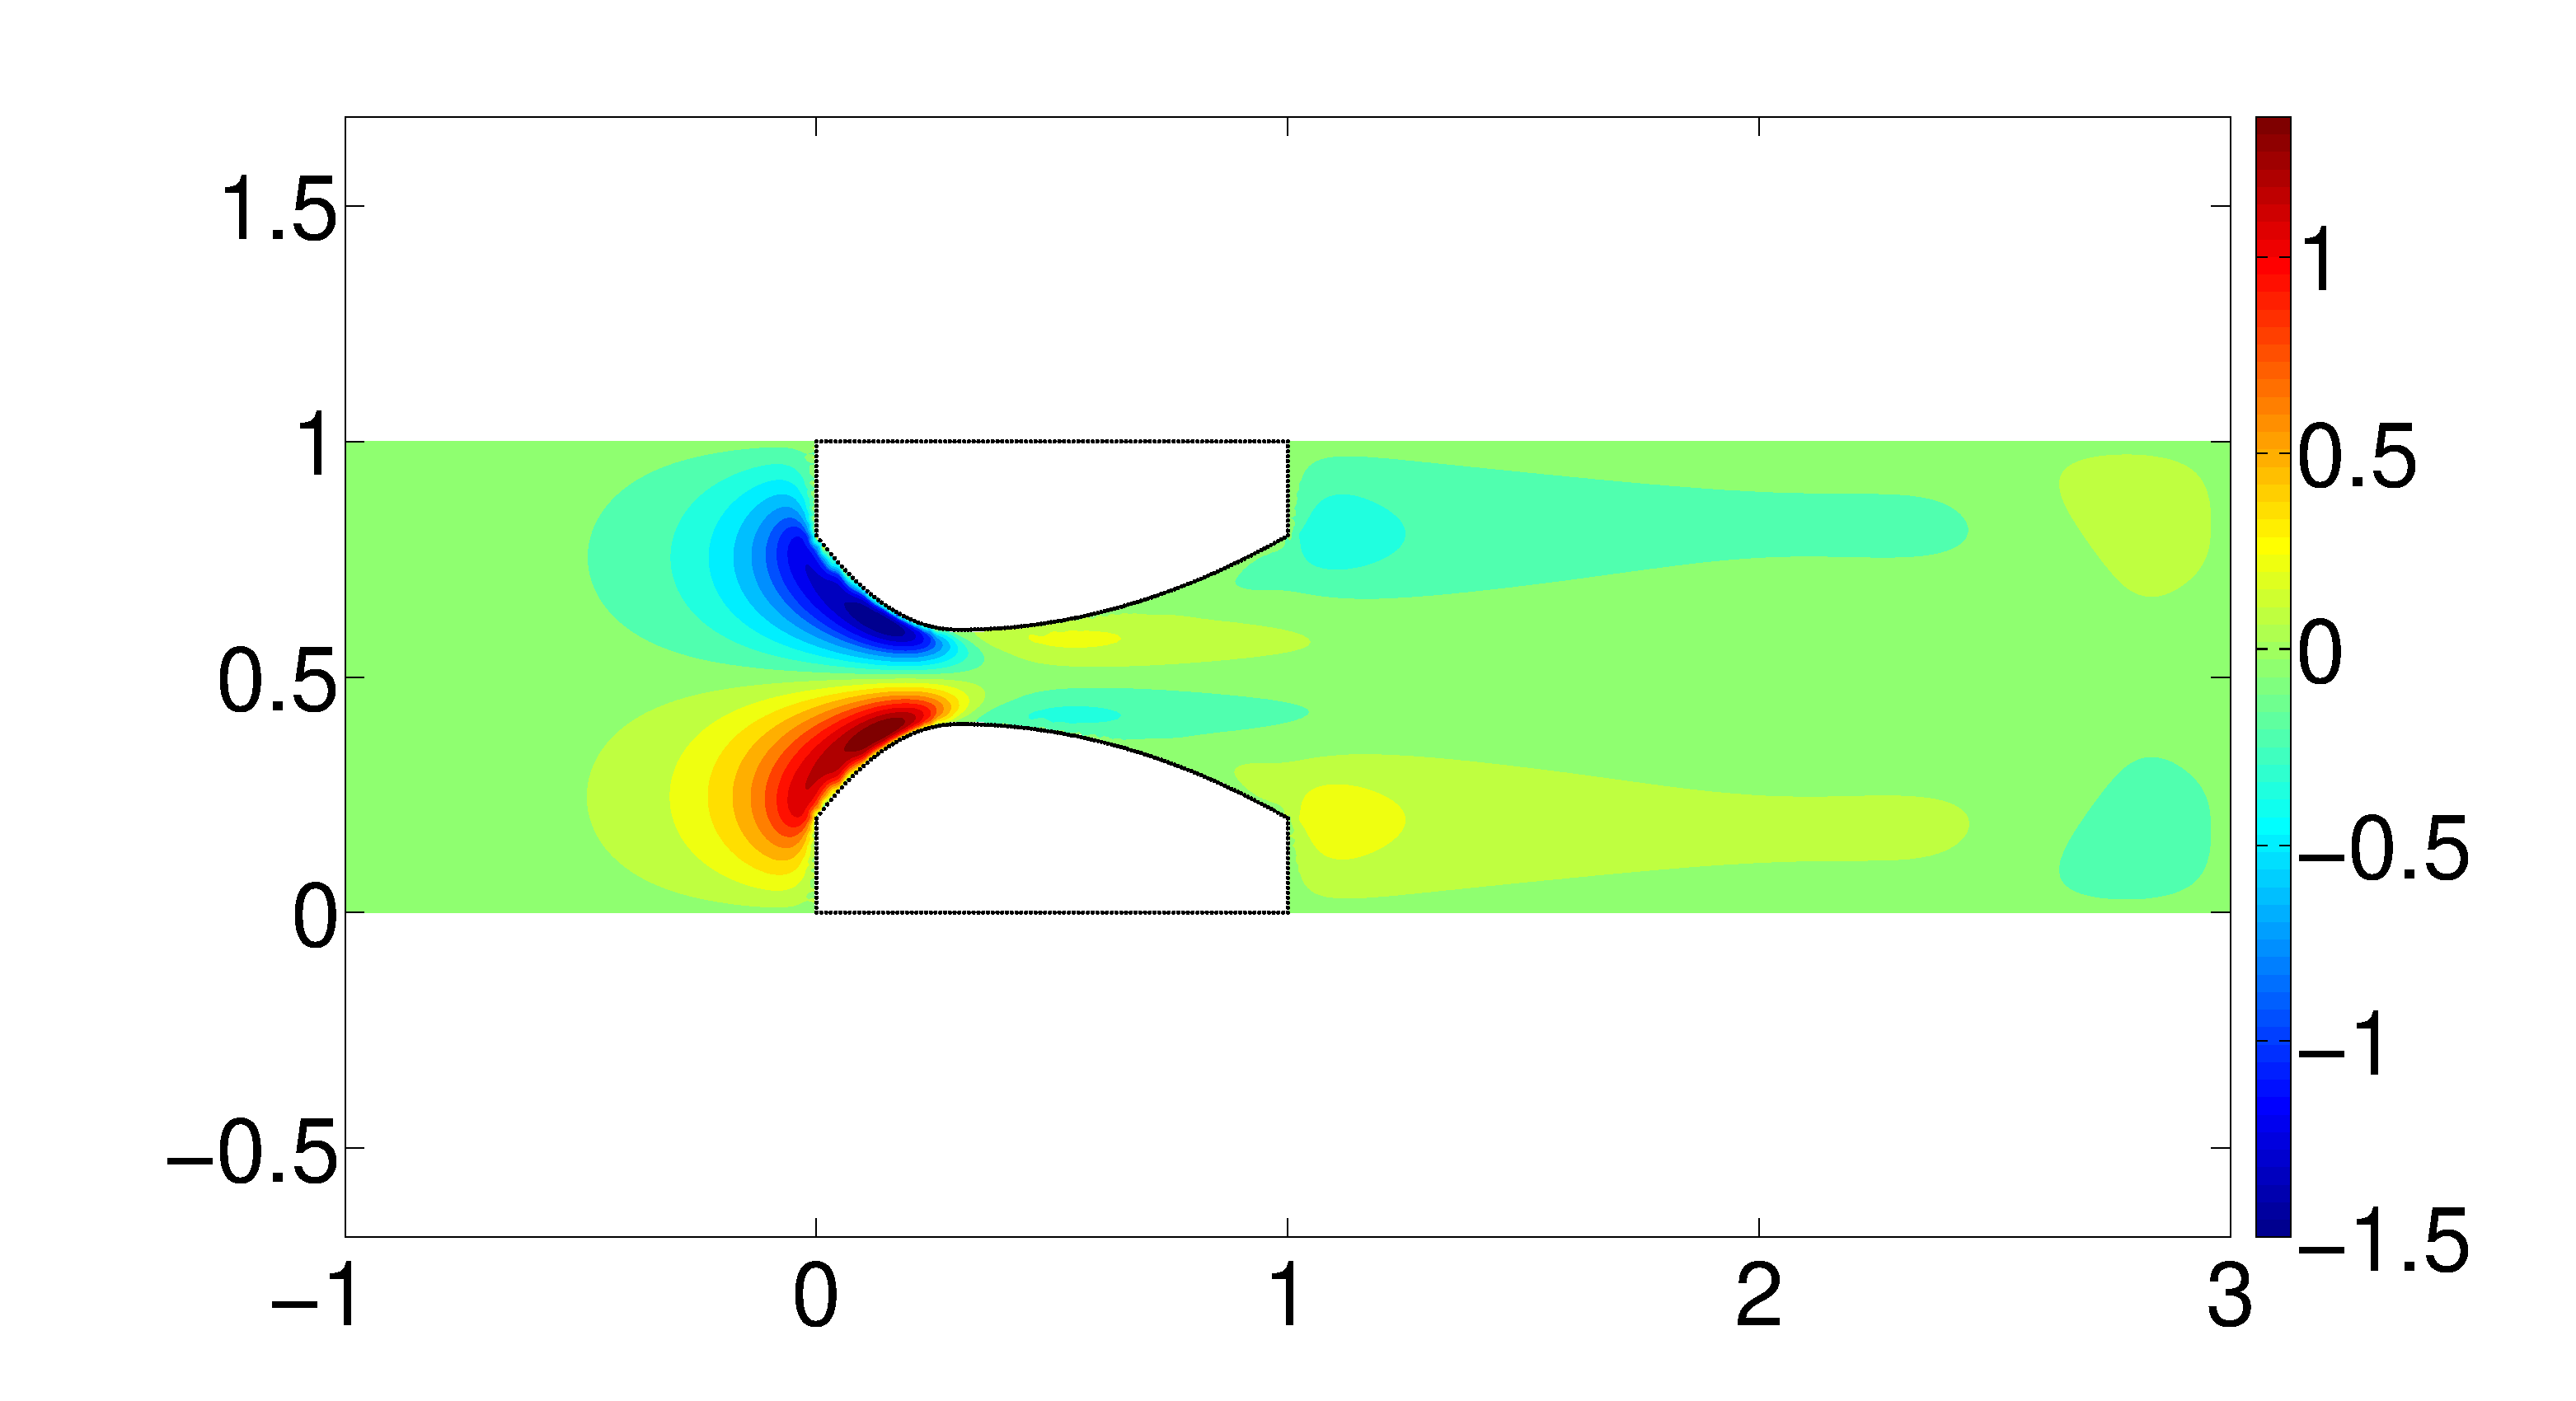
\includegraphics[width=6.5cm]{Chapter_4/figure/flow_through_nozzle/contour_V_RE100.eps}
    }
    \caption{Contour plots for flow through nozzle (Re = 100).}
    \label{fig:C4_nozzleFlow_contourForAnalysis}
\end{figure}
%
The sensitivity of the flow variables with respect to the throat area is calculated by differentiating the governing equations with respect to the design variable. The boundary conditions do not depend on the shape design variable; therefore, their derivative is equal to zero. This results in zero boundary conditions for the sensitivity equations.

The sensitivity of the flow with respect to the throat area is calculated using CSA. The u-velocity and pressure sensitivities are plotted on the symmetry line of the nozzle; whereas, the v-velocity sensitivity is plotted at the throat area. These values are verified with the complex step results where they showed a favorable comparison.
%
\begin{figure}[H]
    \centering
    \subfigure[U-velocity sensitivity.]
    {
    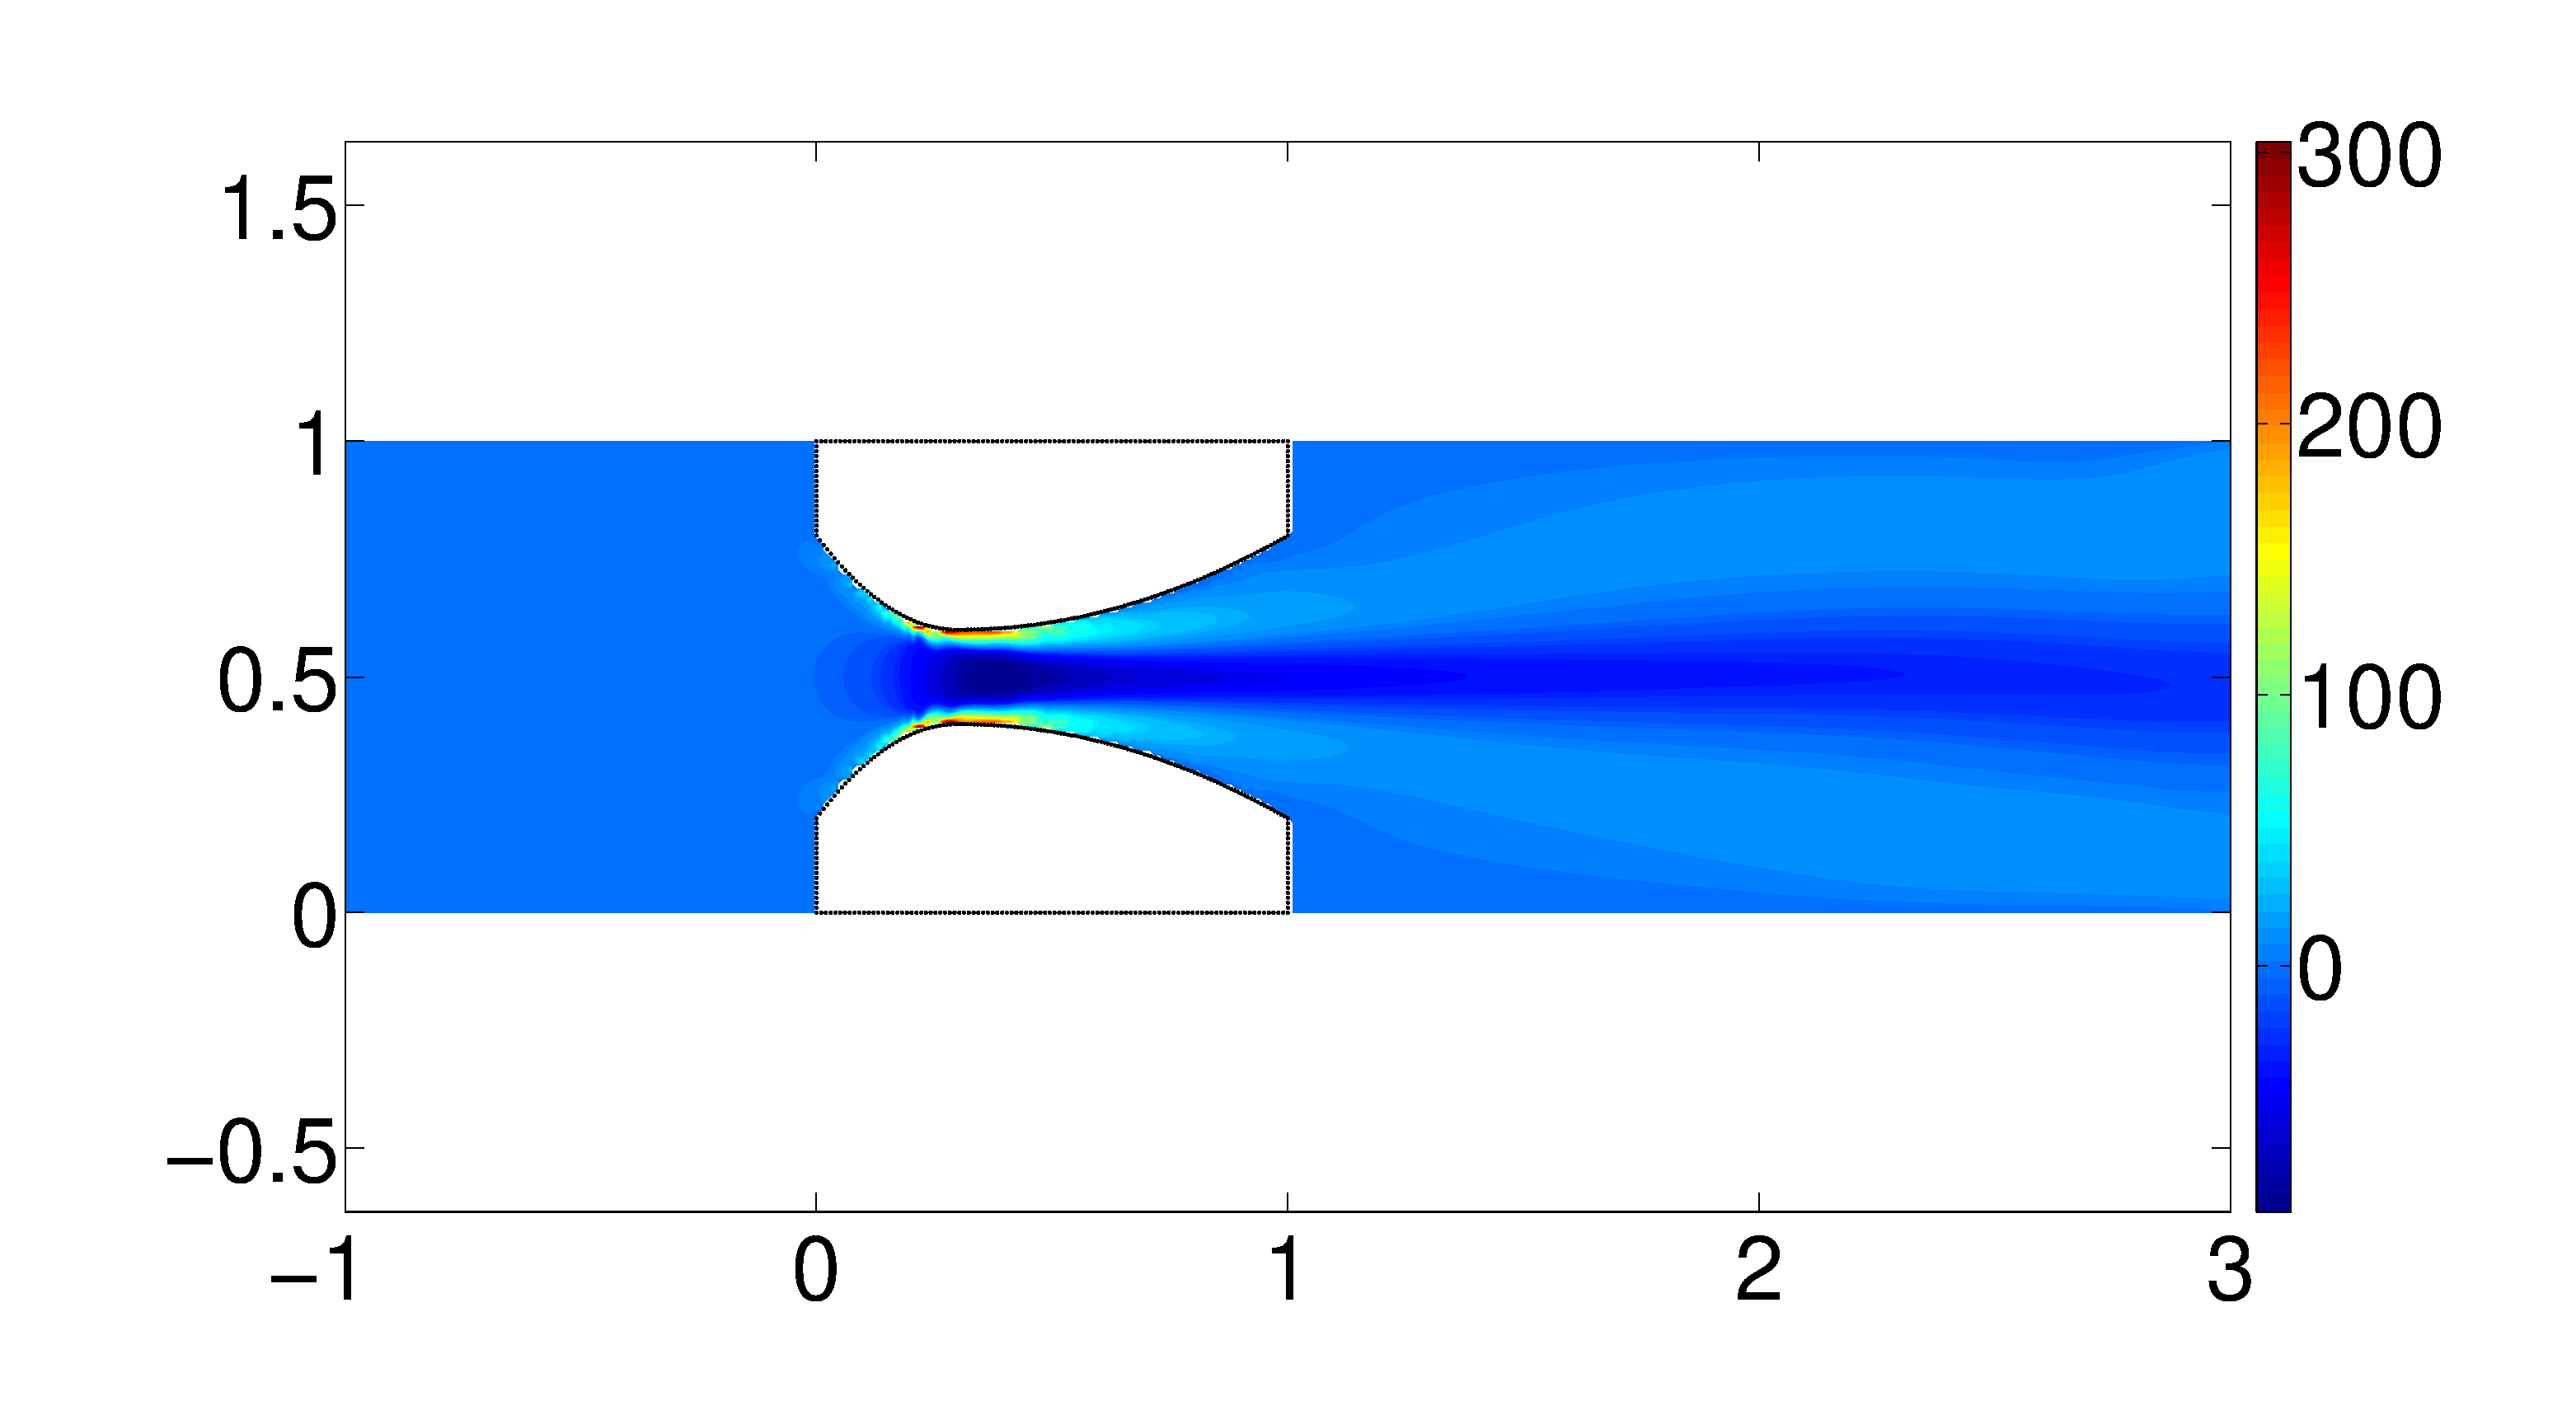
\includegraphics[width=6.5cm]{Chapter_4/figure/flow_through_nozzle/contour_dUdr_RE100.eps}
    }
    \quad
    \subfigure[V-velocity sensitivity.]
    {
    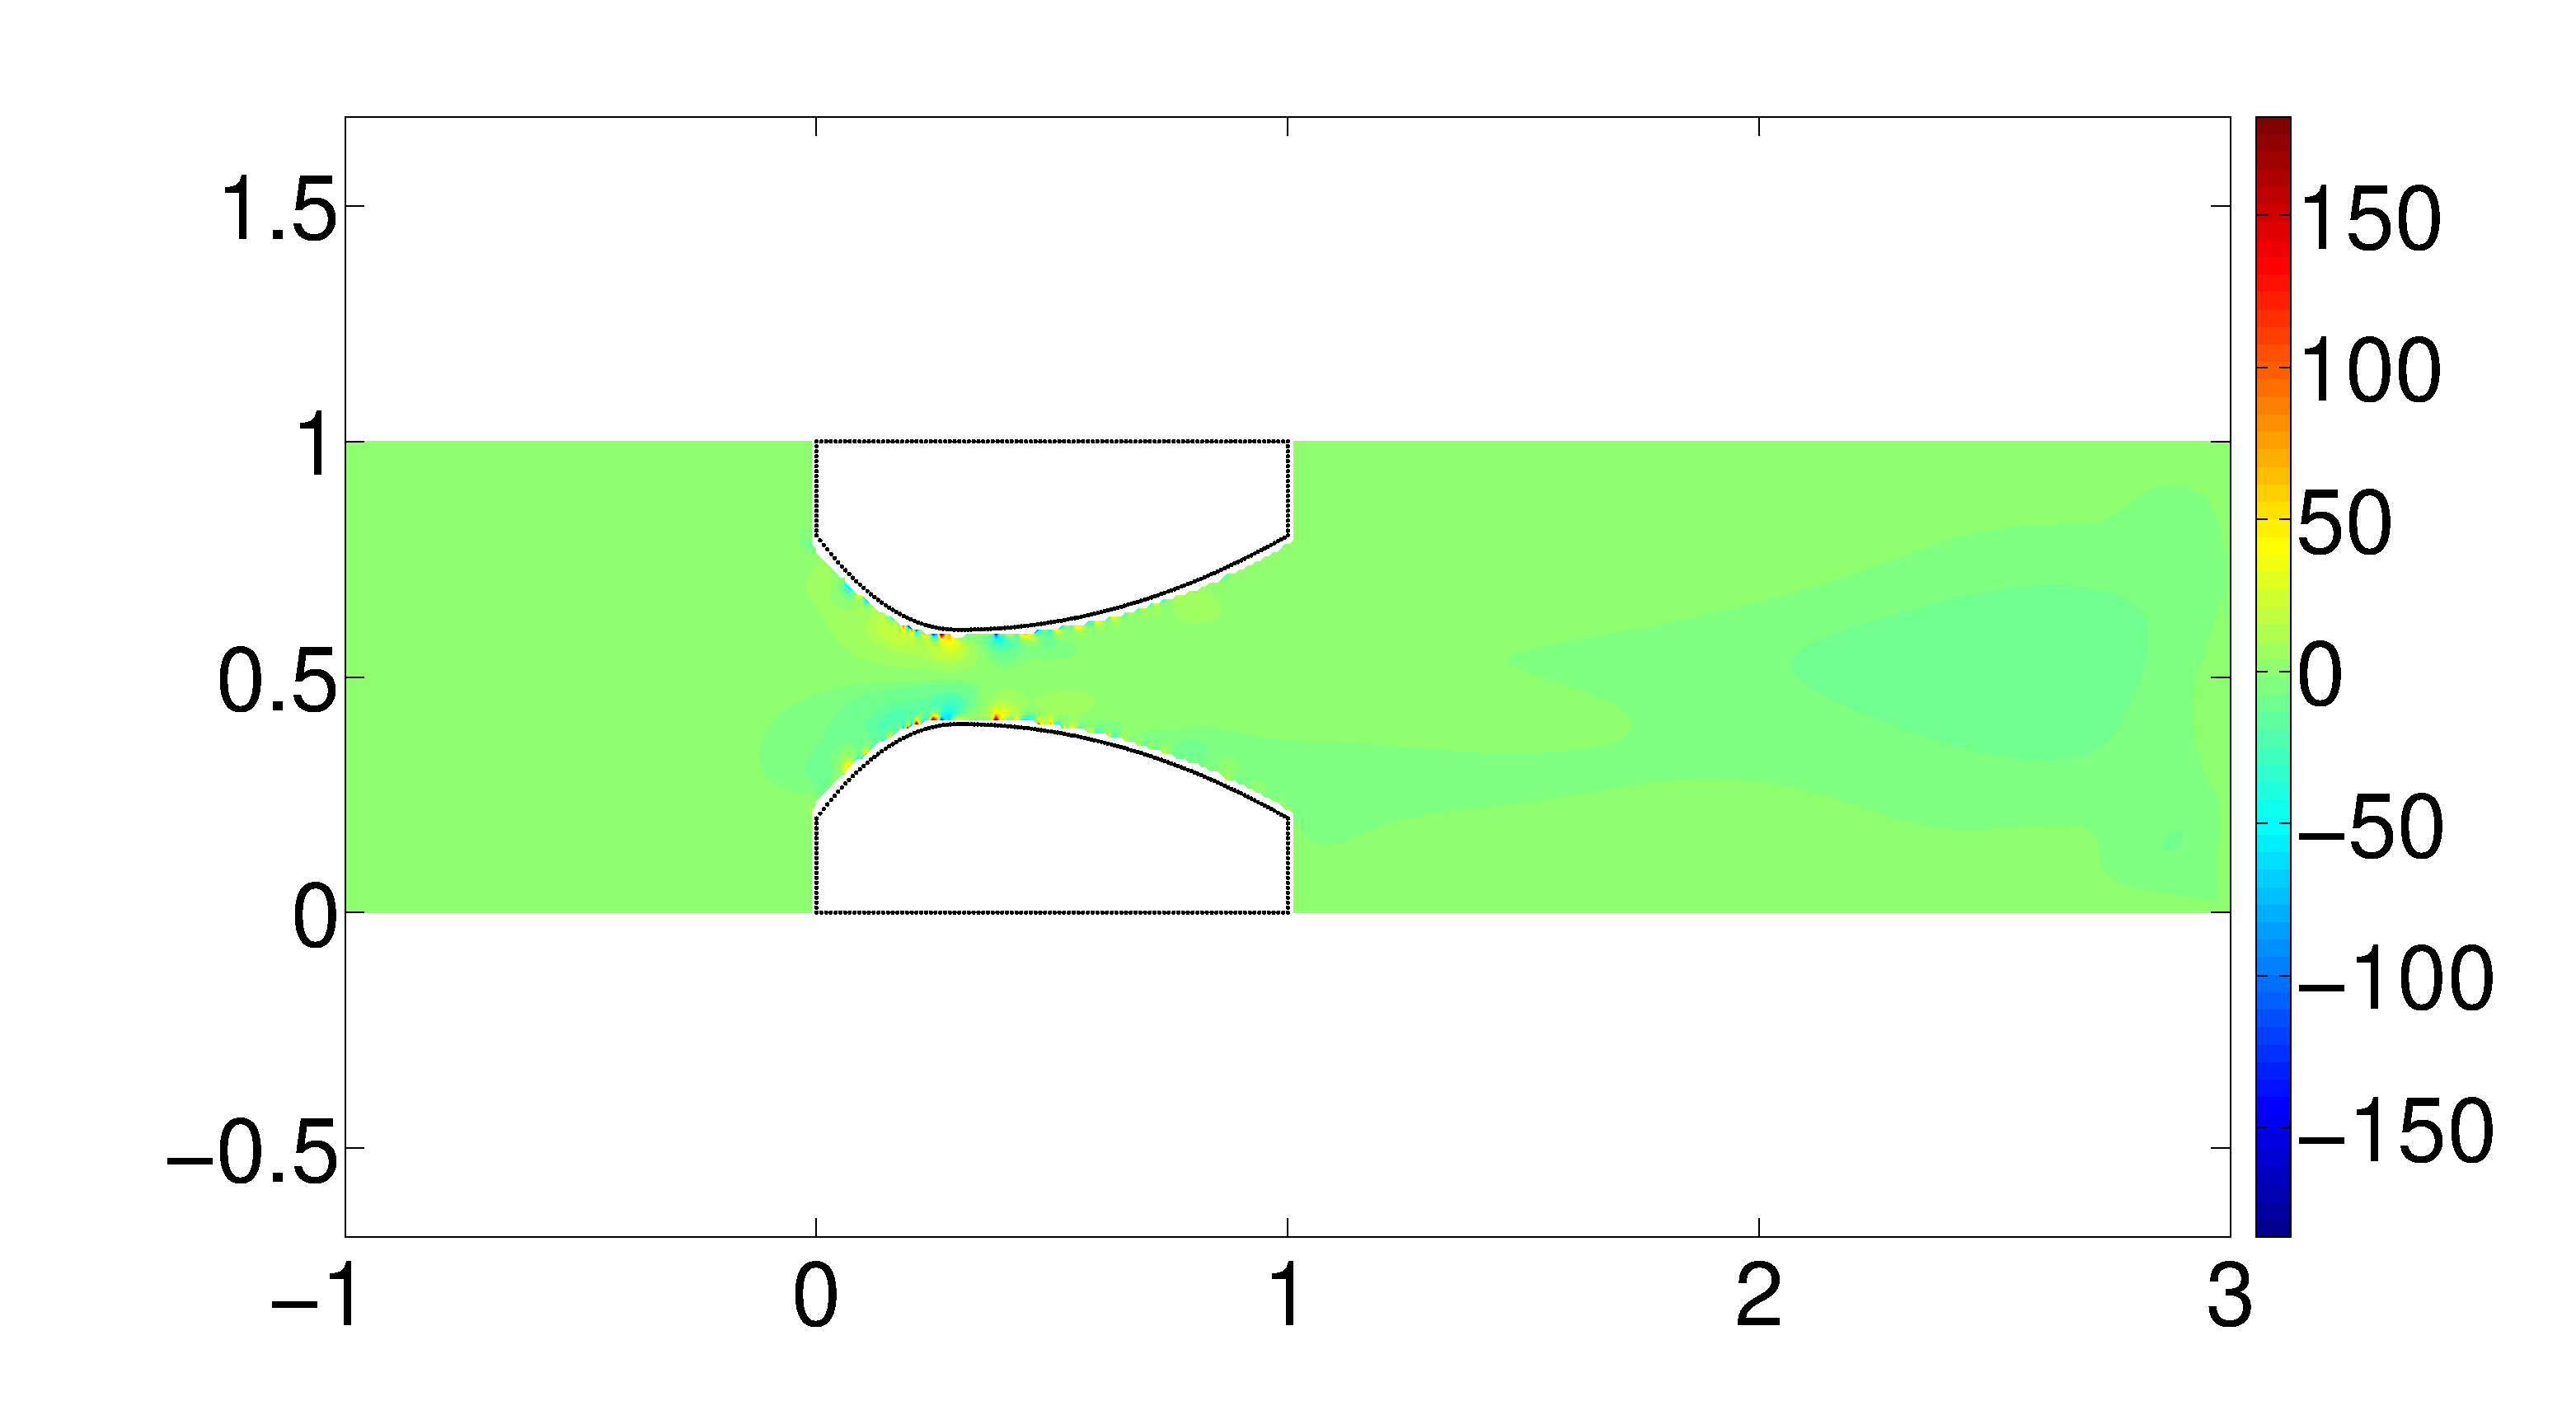
\includegraphics[width=6.5cm]{Chapter_4/figure/flow_through_nozzle/contour_dVdr_RE100.eps}
    }
    \\
    \subfigure[Pressure sensitivity.]
    {
    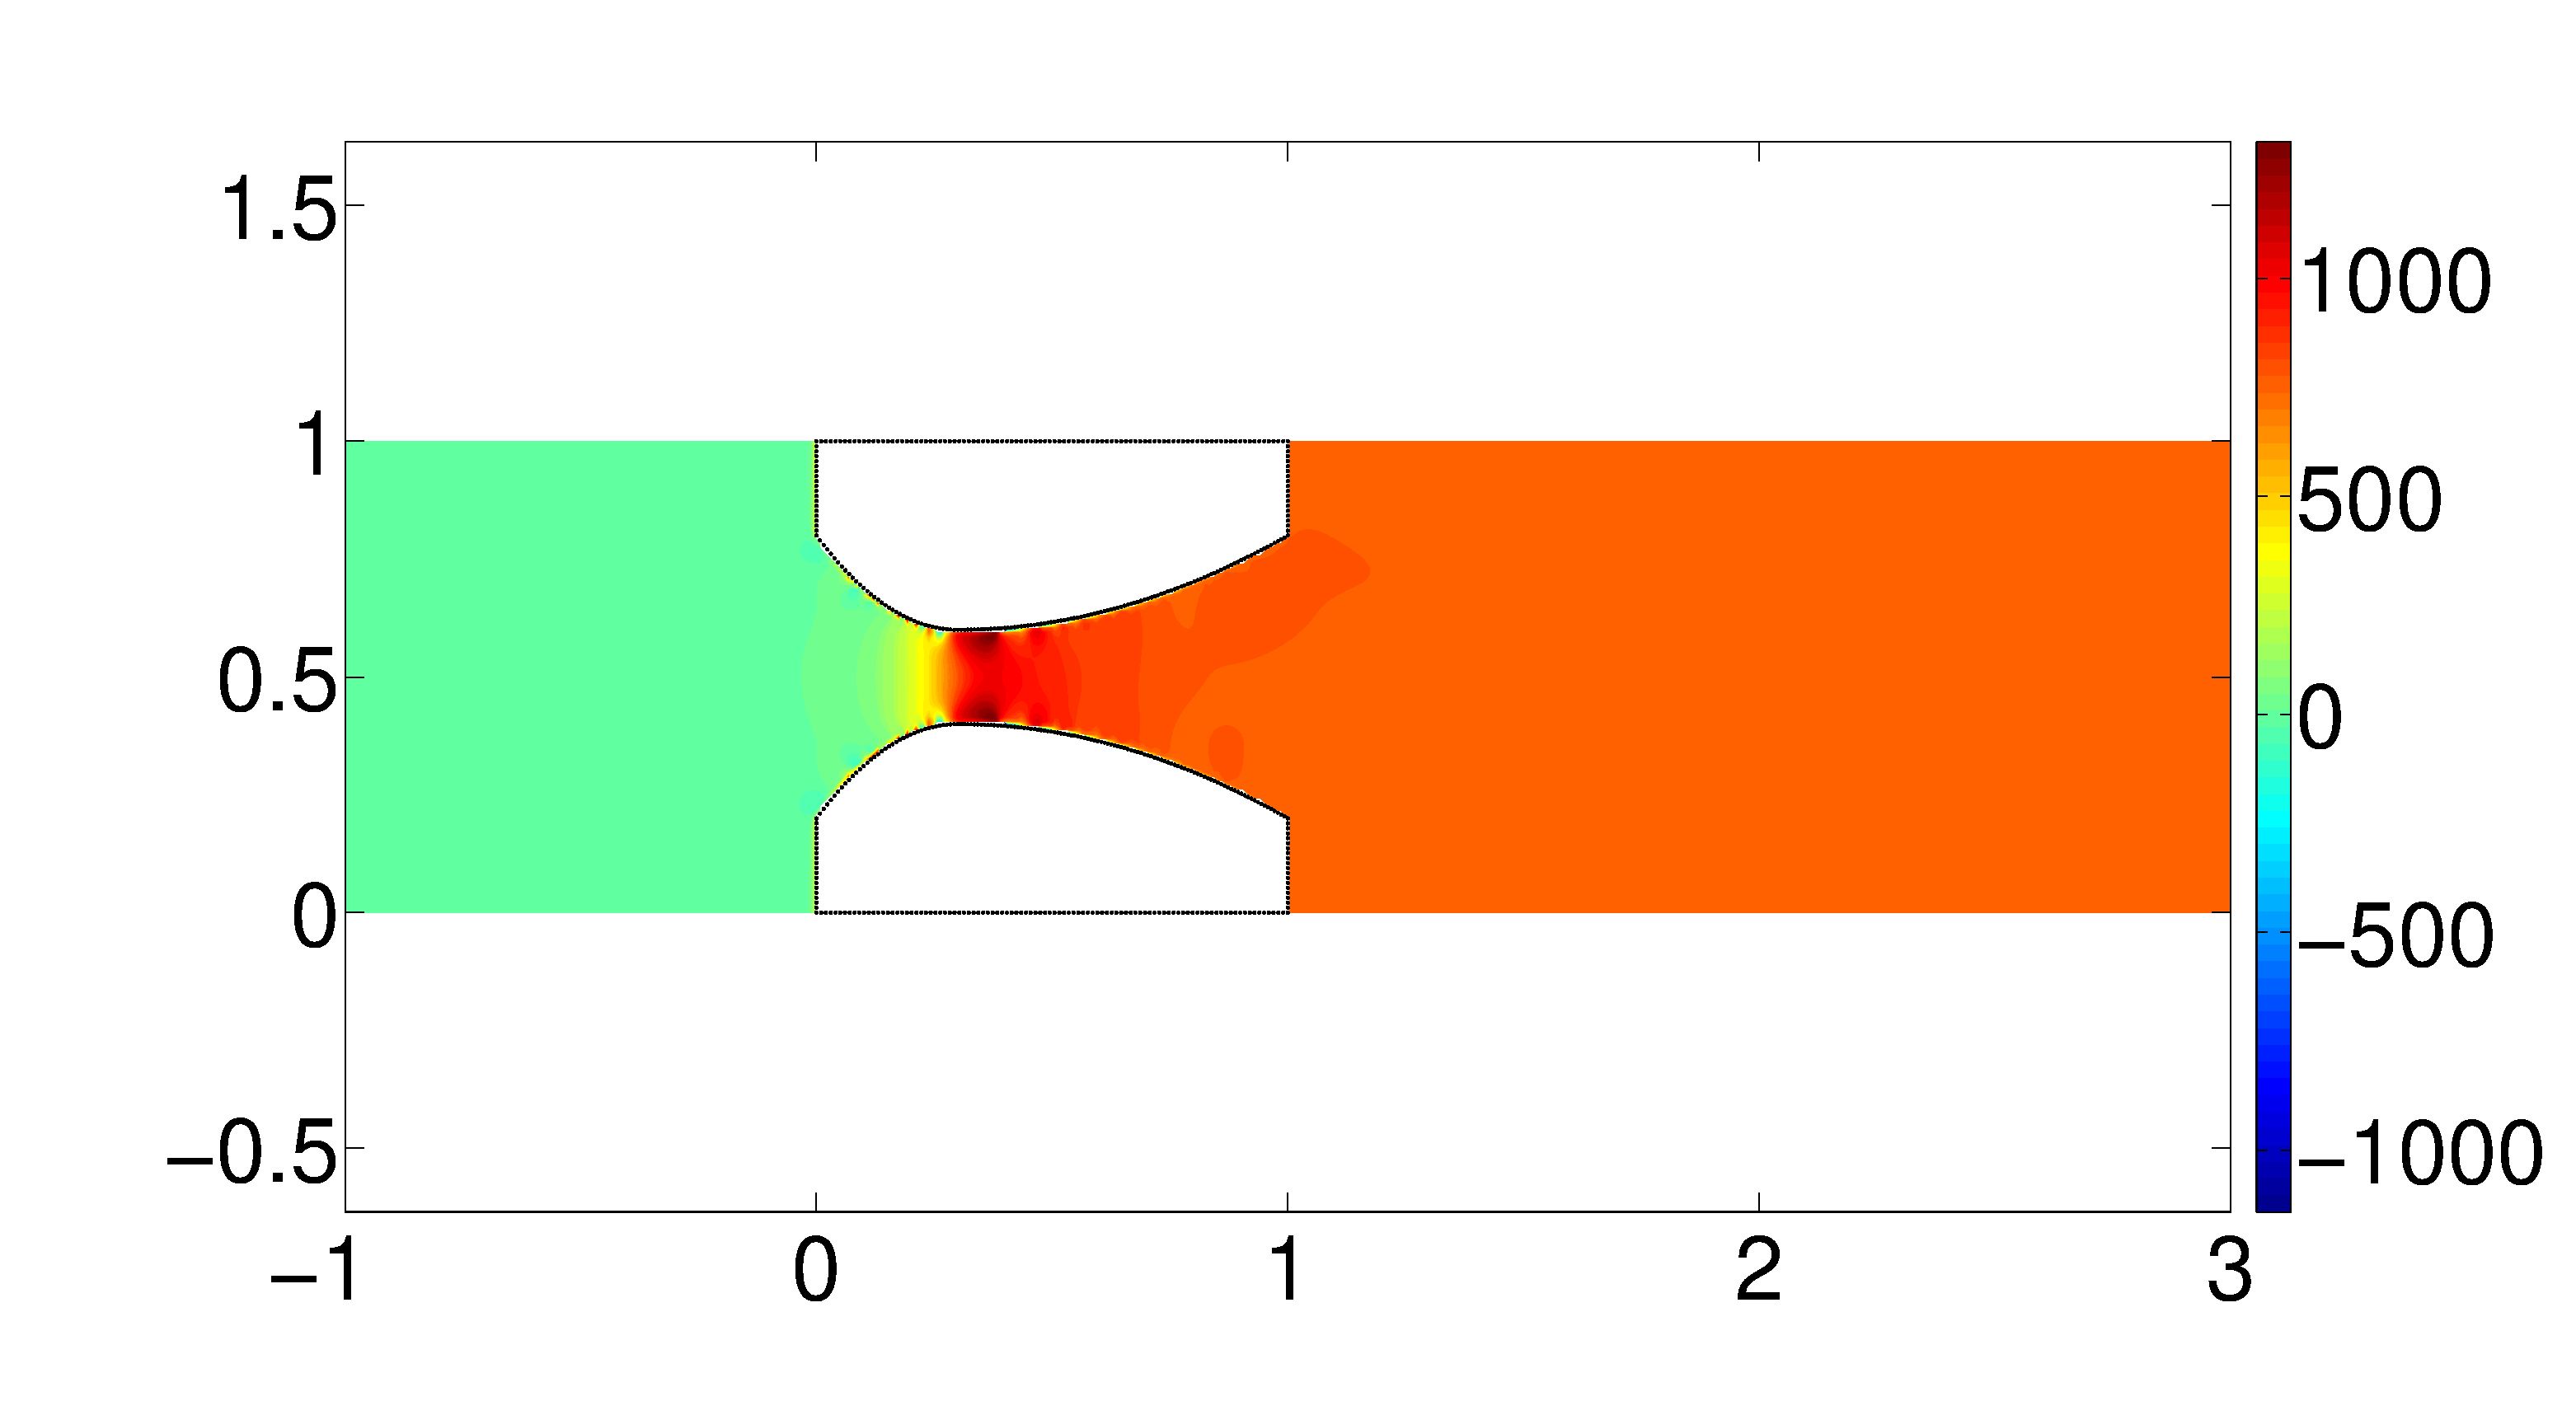
\includegraphics[width=6.5cm]{Chapter_4/figure/flow_through_nozzle/contour_dPdr_RE100.eps}
    }
    \caption{Sensitivity contours.}
    \label{fig:C4_nozzleFlow_sensitivityPlots}
\end{figure}
%
To verify the sensitivity analysis, the sensitivities of velocity and pressure are plotted on different locations in the domain. We chose the symmetry line of the nozzle to plot the u-velocity and pressure sensitivity with respect to the throat are and the vertical line passing through the throat for verifying the v-velocity sensitivity. The verification is done using the complex step sensitivities as shown in Figure \ref{fig:C4_nozzleSensitivityVerification}.
%
\begin{figure}[H]
    \centering
    \subfigure[U-velocity sensitivity on $y = 0.5$.]
    {
    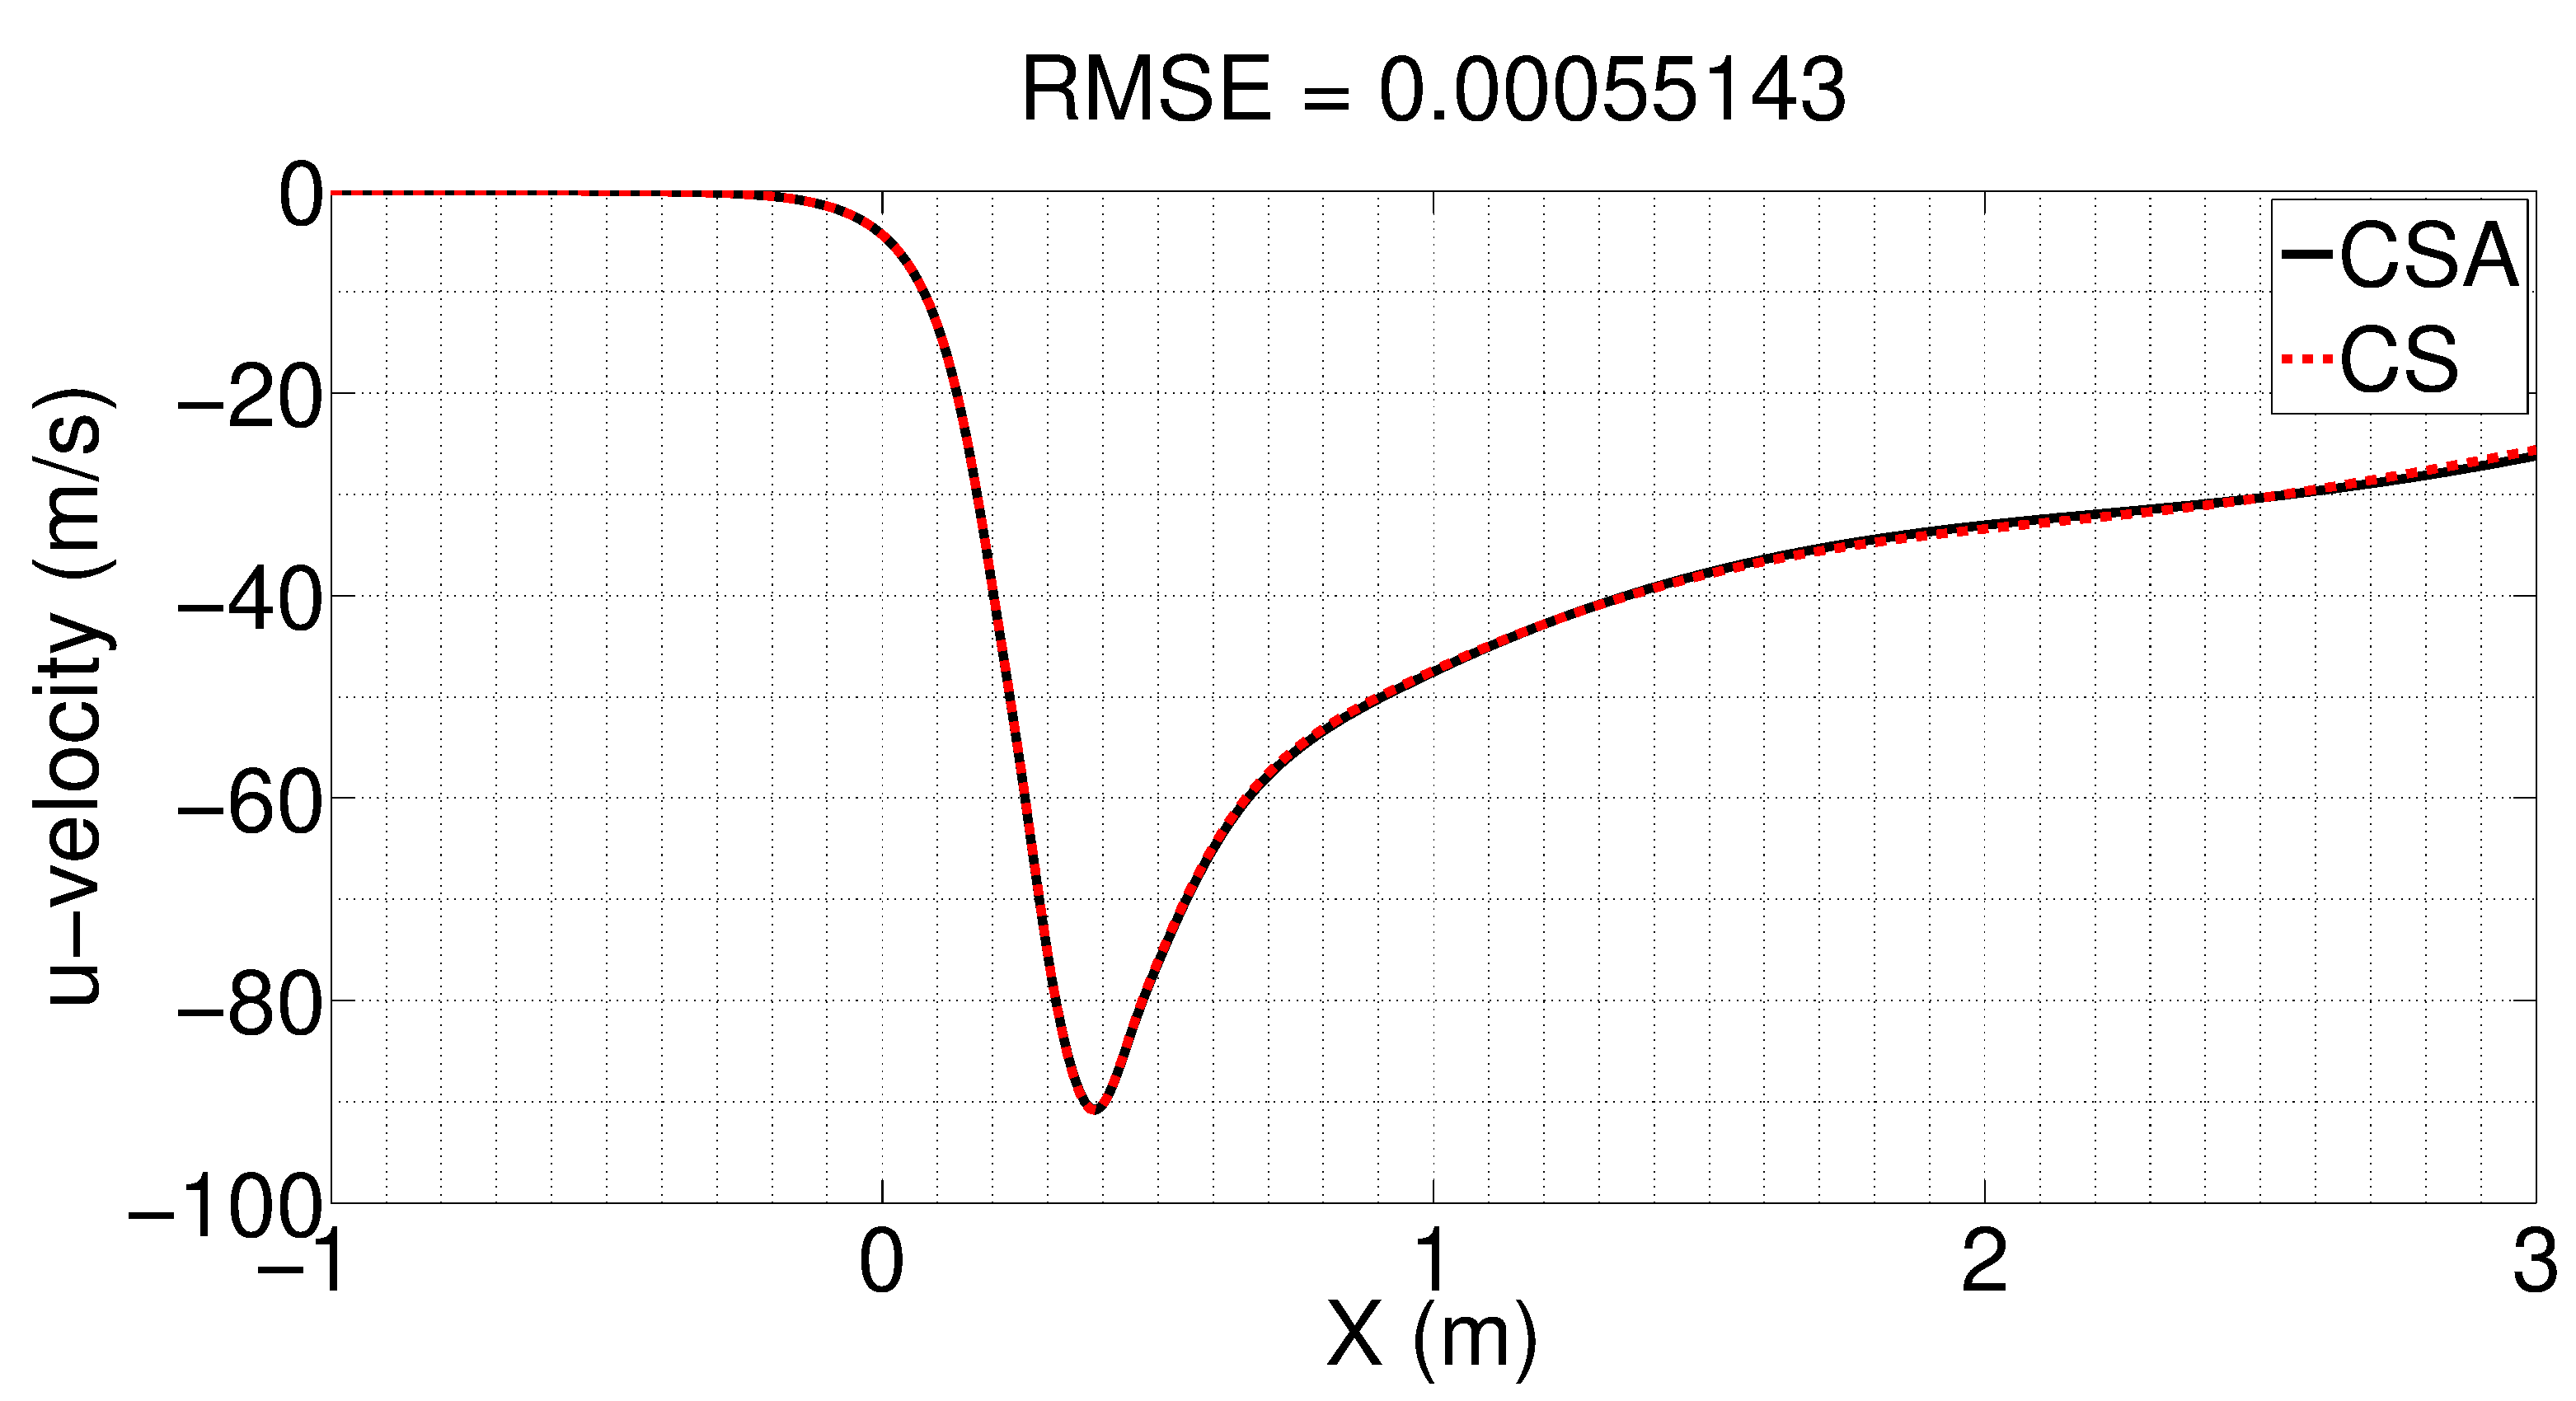
\includegraphics[width=6.5cm]{Chapter_4/figure/flow_through_nozzle/verification_dUdr_RE100_Y050.eps}
    }
    \quad
    \subfigure[V-velocity sensitivity on $x = 0.3$.]
    {
    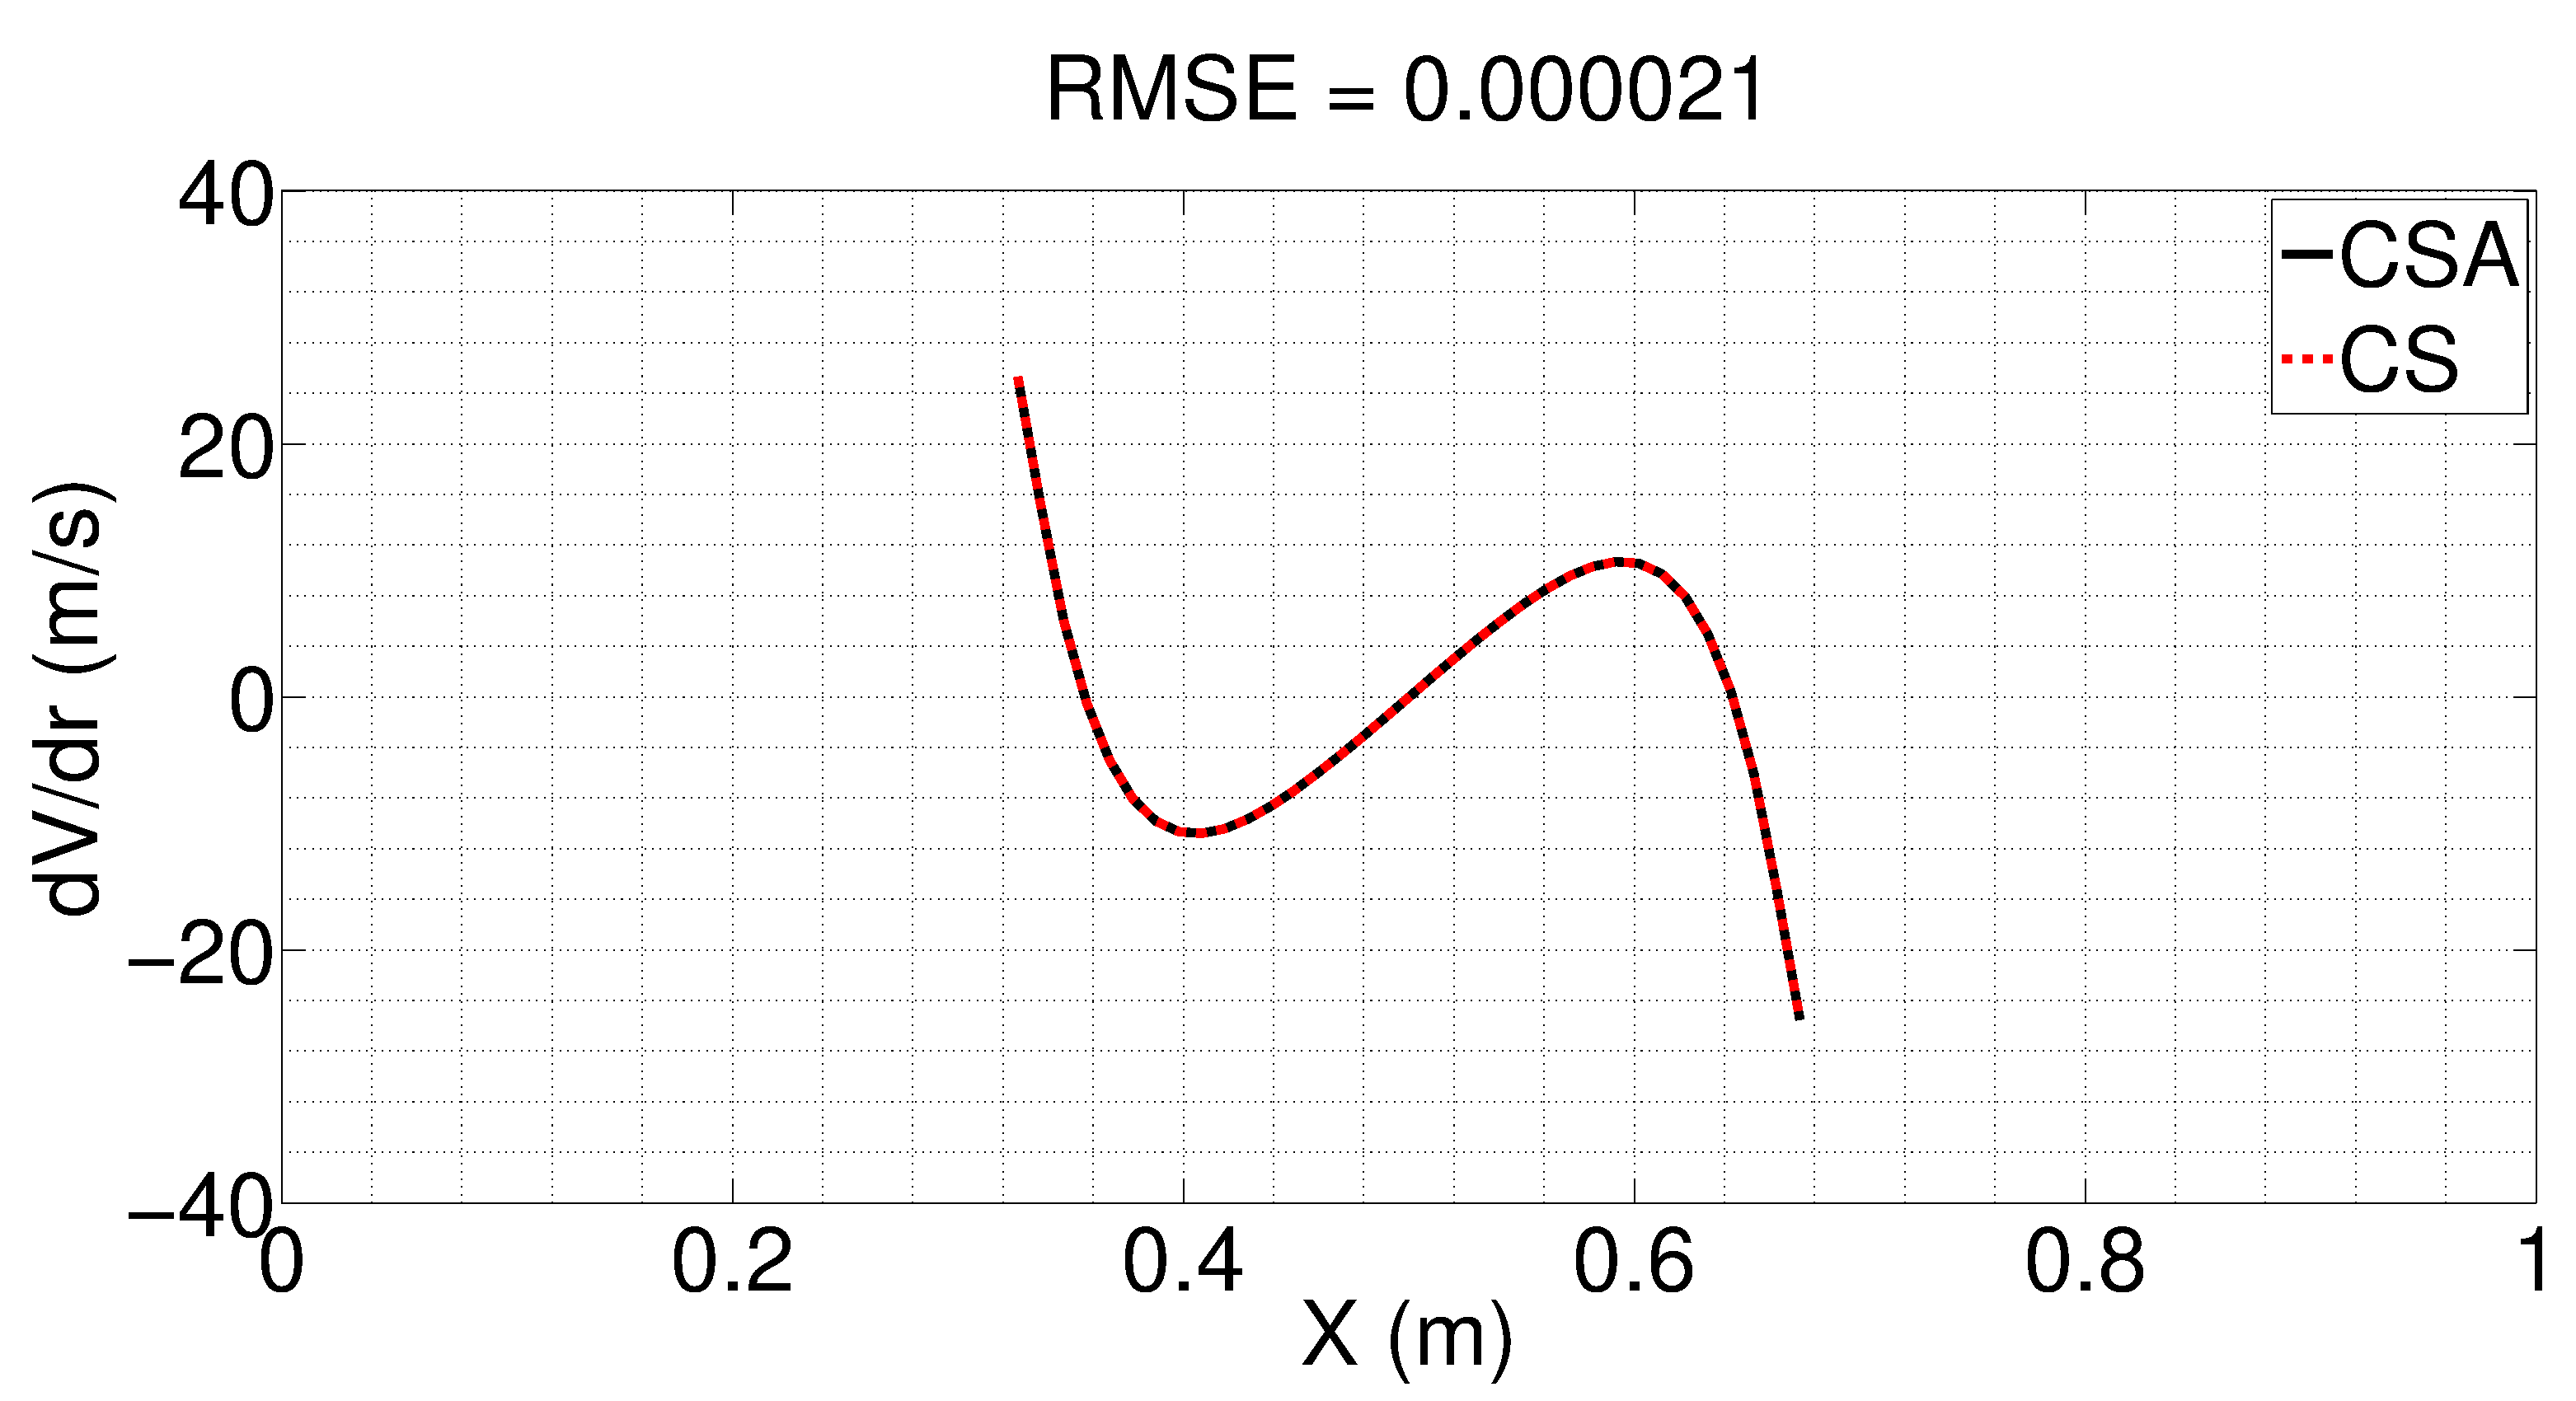
\includegraphics[width=6.5cm]{Chapter_4/figure/flow_through_nozzle/verification_dVdr_RE100_X030.eps}
    }
    \\
    \subfigure[Pressure sensitivity on $y = 0.5$.]
    {
    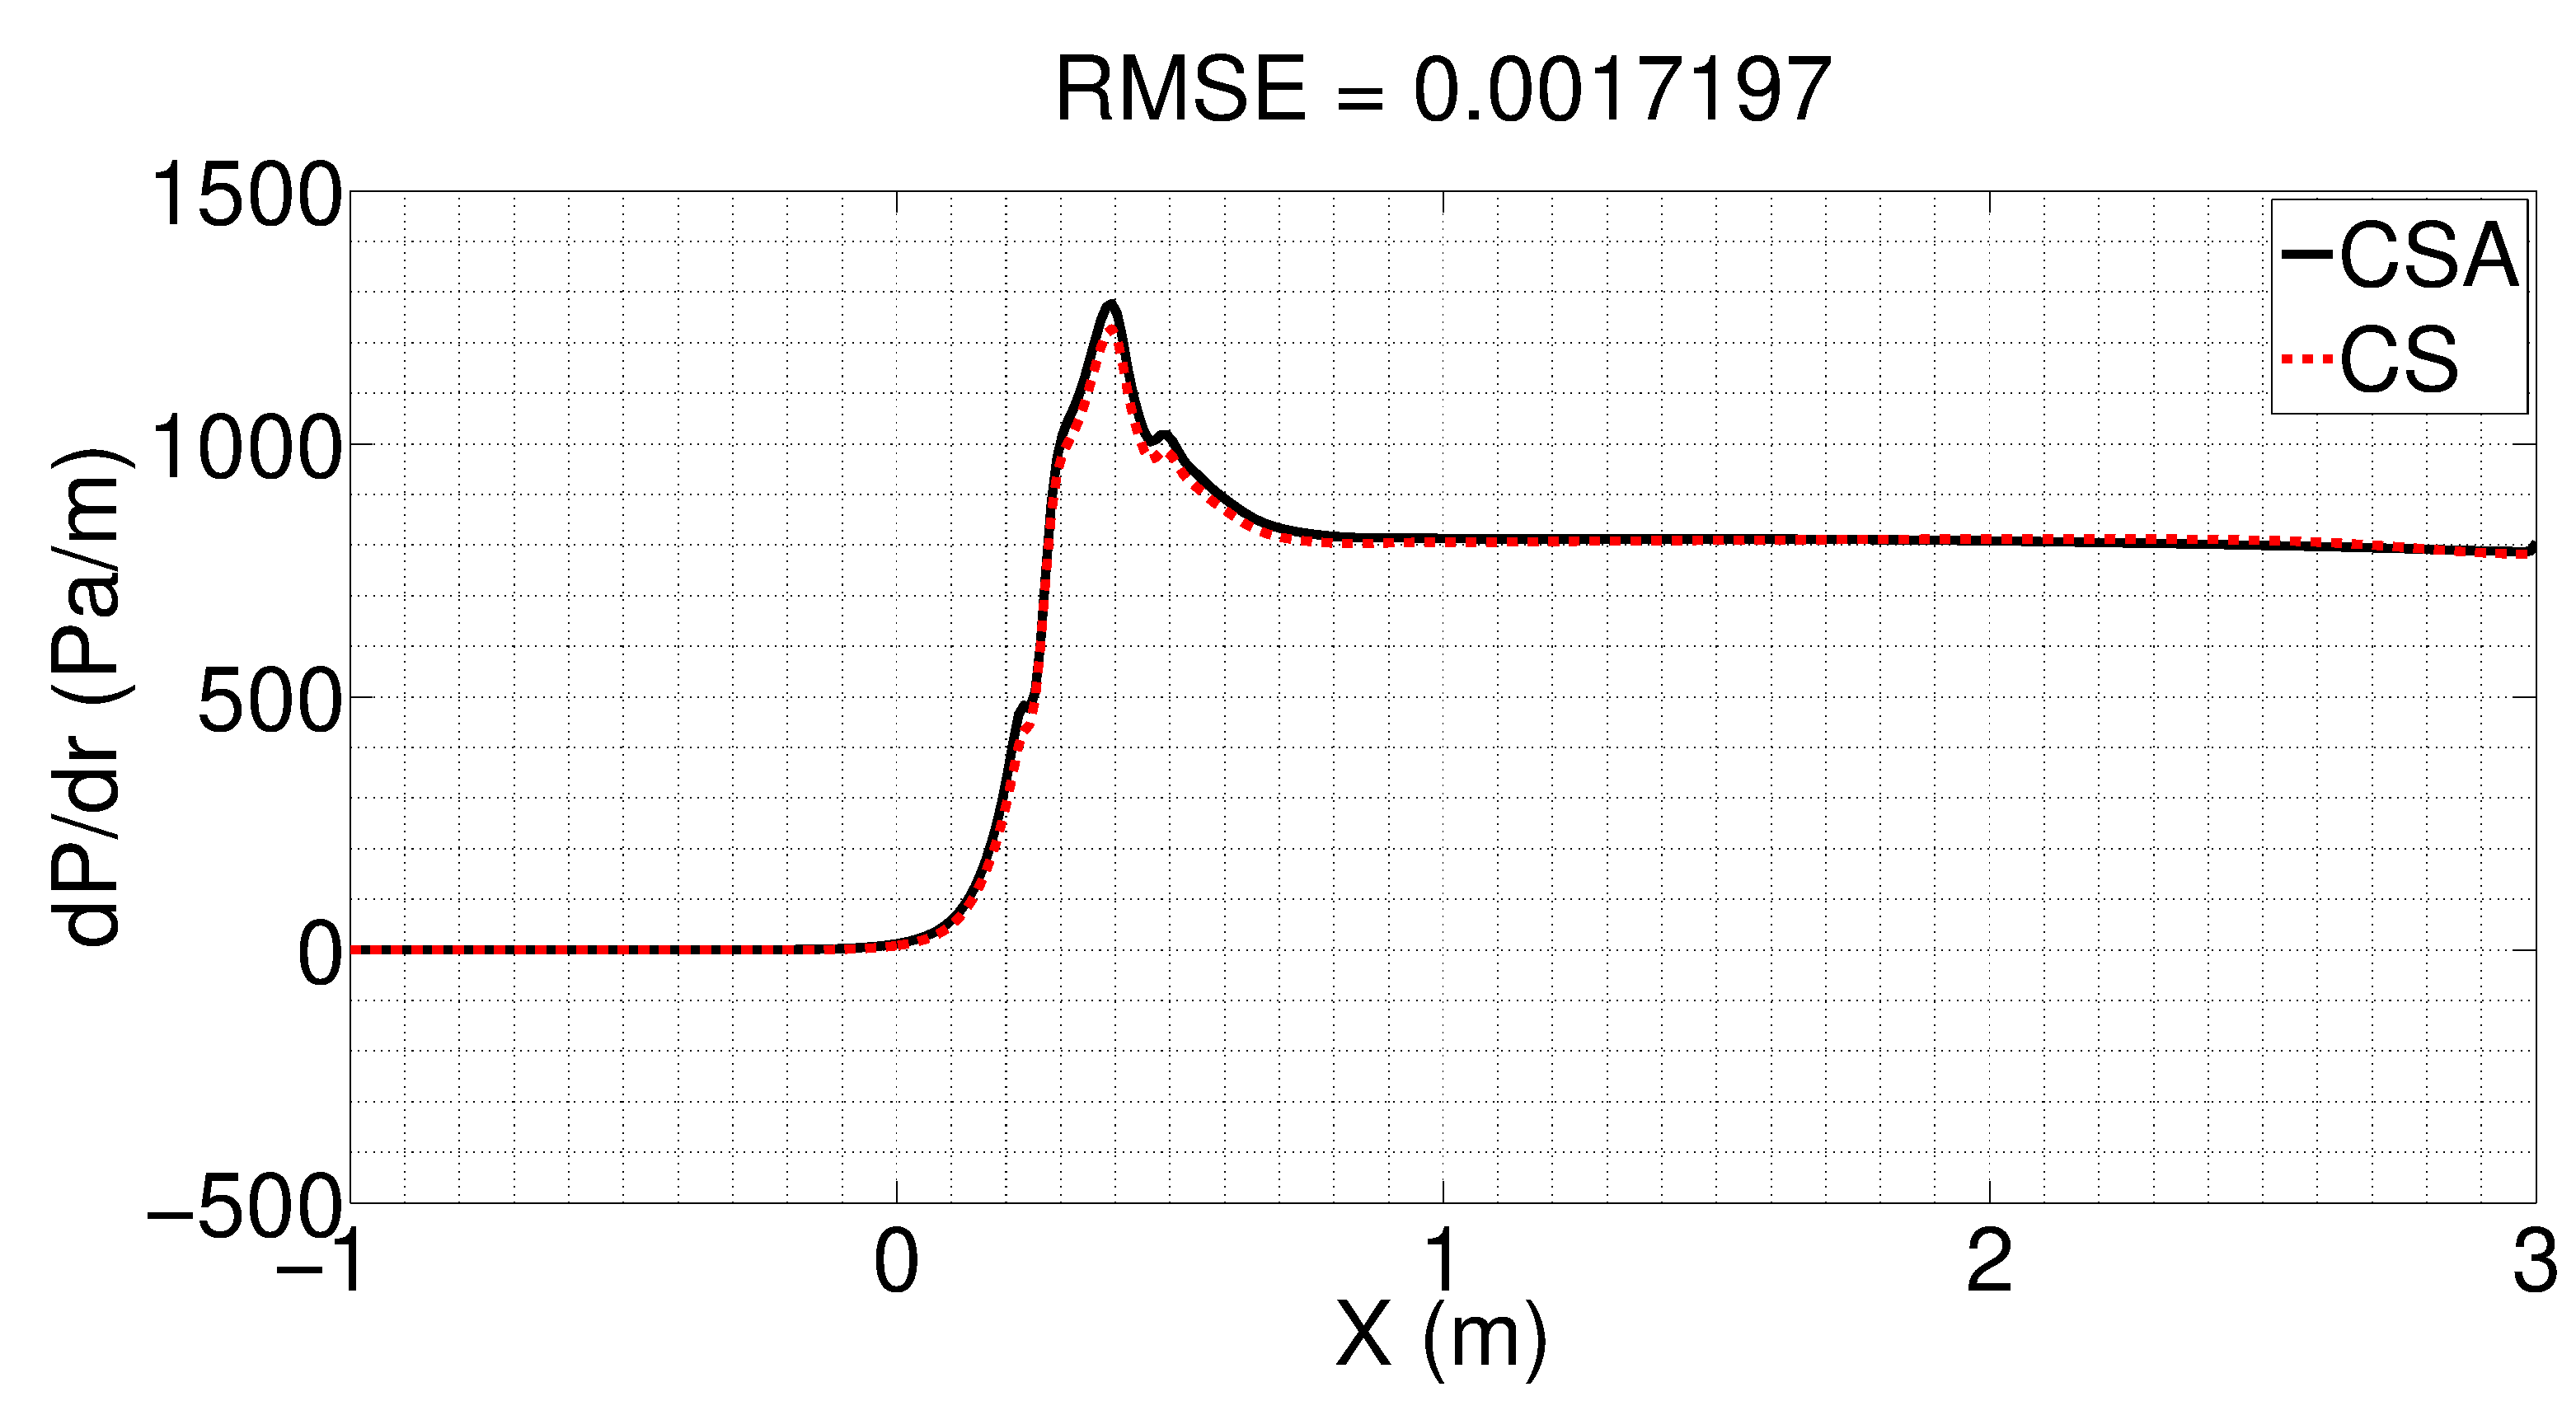
\includegraphics[width=6.5cm]{Chapter_4/figure/flow_through_nozzle/verification_dPdr_RE100_Y050.eps}
    }
    \caption{Verification of sensitivity results for the nozzle.}
    \label{fig:C4_nozzleSensitivityVerification}
\end{figure}
%
% ======================================================================
\section{Summary}
In this chapter, the Continuum Sensitivity Analysis (CSA) framework was applied to the Immersed Boundary (IB) formulation of flow over solid boundaries. In the conventional IB method, Heaviside and Delta functions are used to assign force terms to the governing equations to represent the effect of solid boundaries. To derive the sensitivity equations using the CSA, the governing equations need to be continuously differentiable; however, this is not true for conventional IB formulation. To address this issue, we introduced Regularized Heaviside (RH) and Regularized Delta (RD) functions to the governing equations. These functions are continuously differentiable and are tuned based on the grid size used in the simulation. The governing Navier-Stokes (NS) equations are rewritten based on which two different continuous IB formulations and differentiated to get the sensitivity equations. To get accurate sensitivity response, it is required to use higher-order boundary definition. The sensitivity equations were solved for the sensitivity of the flow variables with respect to different shape design variables where the results were verified using the complex step method. It was shown that the CSA results are in good agreement with numerical results of the complex step method. The convergence rate of the sensitivity equations were also compared with the convergence rate of the governing equations. For the conducted analysis, it was reported that the sensitivity equations converge with the same rate as the governing equations.